%%%%%%%%%%%%%%%%%%%%%%%%%%%%%%%%%%%%%%%%%%%%%%%%%%%%%%%%%%%%%%%%%%%%%%%%%%%%%%%%%%%%%%%%%%%
%%
%% The updated version of this document should be downloaded from
%%      https://github.com/jp-um/university_of_malta_LaTeX_dissertation_template
%%
%% In case of any difficulties please contact Prof. JP Ebejer on jean.p.ebejer@um.edu.mt
%%
%%%%%%%%%%%%%%%%%%%%%%%%%%%%%%%%%%%%%%%%%%%%%%%%%%%%%%%%%%%%%%%%%%%%%%%%%%%%%%%%%%%%%%%%%%%

%% Before you embark on this quest you should probably read some of:
%% Deadly sins - http://mirrors.ctan.org/info/l2tabu/english/l2tabuen.pdf
%% Writing a thesis in LaTeX - http://tug.org/pracjourn/2008-1/mori/mori.pdf

\RequirePackage[l2tabu, orthodox]{nag} % tells you of any bad LaTeX usage
                                       % must be first thing in class (with the exception of comments)
\RequirePackage{placeins}		       % To use \FloatBarrier

%% There is one option you should define; oneside or twoside.
%% By default all electronic submissions should be `oneside`
%% Use twoside for printing (e.g. the supervisor's customary copy)
%% Note that margins will change accordingly and automatically
\documentclass[oneside]{nus}  % custom National University of Singapore project/dissertation/thesis 
\usepackage[a4paper,margin=1in,heightrounded]{geometry} %control margins explicitly
% \usepackage[showframe]{geometry} %for debugging; draws boxes so you can see whether inner/outer margins differ
%% \counterwithout{footnote}{chapter} % use this to have continuous numbering for your footnotes (that do not reset per chapter)

%% **************** (Your) Packages (Start) ******************

% \listfiles % uncomment this to know which packages you are using
              % the list of packages will be in the bottom of the .log file

%% Note that packges may already be loaded from the nus (and memoir) classes.
%% Do not add your packages to the template, but rather add them here.

\usepackage{blindtext} %% for some dummy text, remove in your writeup
\usepackage{coffee4}    %% for some fun
% ---------- Listings + Code fonts ----------
\usepackage[T1]{fontenc}
\usepackage[scaled]{inconsolata}   % nicer monospace
\usepackage{listings}
\usepackage{xcolor}
\usepackage{hyperref}
\usepackage{enumitem}
\usepackage{graphicx}
\usepackage{url}
\usepackage{tikz} %to draw figures
\usetikzlibrary{arrows.meta,positioning,fit,shadows.blur,calc}
\usepackage{adjustbox}
\usepackage{caption}
\usepackage[most]{tcolorbox}

% Listings style (no frame breaks, safe line breaks)
\lstdefinestyle{finsight}{
  basicstyle=\ttfamily\small,
  numbers=left,
  numbersep=8pt,
  stepnumber=1,
  frame=single,
  framerule=0.4pt,
  breaklines=true,
  breakatwhitespace=true,
  tabsize=2,
  showstringspaces=false,
  captionpos=b,
  keepspaces=true
}
\lstset{style=finsight}

% after \usepackage[backend=biber,style=authoryear]{biblatex}
\renewcommand*{\mkbibparens}[1]{\mkbibbrackets{#1}} %render square brackets instead of circlular for \parencite

%% ***************** (Your) Packages (End) *******************


%% **************** (Your) Data (Start) ******************

\title{FinSight:\\Intelligent Stock Prediction\\and Advisory Platform}  % use \\ here otherwise you get a justified title
                                     % note capitalization of the title (only common 
                                     % words in lower case)
\tagline{augmenting the lives of finance professionals}      % tag line *OPTIONAL* 
\author{\vspace{5 pt}Huo Yiming (A0328696J) \\ \vspace{5 pt}Li Jiajun (A0326795M) \\ \vspace{5 pt}Samarth Soni (A0329960U) \\ \vspace{5 pt}Su Yuxuan (A0329926N) \\ \vspace{5 pt}Wang Yixi (A0328469M)}            % your full name
\authorID{123456M}                   % your University Identifier
\supervisor{Mr.\ Hunarpreet Singh}           % your supervisor(s) name
\cosupervisor{Prof Dr Gary Leung}                % your cosupervisor(s) name - no . in Dr *OPTIONAL* 
                                     % simply comment out the above line if absent
\department{Intelligent Reasoning Systems Graduate Certificate}   % your department (e.g. Artificial Intelligence)
\faculty{Institute of Systems Science}       % your faculty (e.g. ICT)
\degreeName{M.Tech.\ Artificial Intelligence Systems}       % the degree you are reading
                                     % note the \ after the dot, so not to consider it a fullstop
\doctype{dissertation}               % the type of document (fyp, dissertation, thesis)
%%\subjectcode{ICS5200}              % the study unit-code (currently not used)
\submissionDate{\DTMenglishmonthname{\the\month}, \the\year}     % The actual (corrected, post-viva) submission month, inc. year, should probably be fixed.

%% ***************** (Your) Data (End) *******************

%%
\renewcommand{\chapterheadstart}{\vspace*{\beforechapskip}}
\setlength\beforechapskip{0mm}


%% ******** (Your) Document Settings (Start) *************

% You should have an images directory in every chapX subdir
% NOTE:  Trailing / for subdirs is required.
\graphicspath{{./images/}{./chap1/images/}{./chap2/images/}}   % Paths where to look for images, if defined "images" must always be there as it holds the images in-use by the template.

\makeindex

\addbibresource{chap1/introduction_biblio.bib}
\addbibresource{chap2/background_and_lit_overview_biblio.bib}
\addbibresource{chap3/materials_and_methods_biblio.bib}
\usepackage{lmodern} %latin modern
\usepackage{graphicx}
\usepackage{float}       % for [H] exact placement
\usepackage{booktabs}    % nicer tables
\usepackage{tabularx}    % auto-width tables
\usepackage{caption}
\usepackage{pdfpages}

\captionsetup{font=small,labelfont=bf}
\renewcommand{\arraystretch}{1.15}
%% ********* (Your) Document Settings (End) **************

% DOCTOR'S (JP) ORDERS: MAKE SURE TO READ MY TWO BLOG ENTRIES WITH
% CONTENT AND LaTeX TIPS FOR YOUR WRITE-UP.  THESE ARE BASED ON  
% EXAMINER'S FEEDBACK
%
% URLS:
% https://bitsilla.com/blog/2019/03/content-tips-for-your-dissertation-or-project-write-up/
% https://bitsilla.com/blog/2019/01/latex-tips-for-your-dissertation-or-project-write-up/

% end the preamble and start the document

\begin{document}
\frontmatter 
	\maketitle
	\begin{copyrightenv}
\end{copyrightenv}
       
	%% The originality statement is *NOT* part of the dissertation but submitted separately.
	%\begin{dedication}
{\large{To God \& Our Parents}}\\[5mm]
For their unwavering love, constant support, and steadfast belief in our success which made this endeavour possible.
\end{dedication}

        % include a dedication.tex file
	\begin{acknowledgements}
At the outset, we would like to express our gratitude to our professors Prof Gary Leung, Prof Zhu Fangming, Prof Liya Ding, Prof Xavier Xie, Prof Barry Shepherd, Prof Fan Zhenzhen, Prof Tian Jing, Prof Wang Aobo for imparting unto us the critical knowledge required for us to deliver effective results in this project. Their in-depth instruction and carefully curated teaching and workshops helped us in identifying areas to work on and techniques to utilise. We would like to acknowledge the entire staff at NUS ISS for making our onboarding to the course smooth and full of enthusiasm and engagement. We also wish to acknowledge the inviting and open collaborative culture in our course, which has made us feel at home and empowered to do our academic work with full focus.

We would like to especially acknowledge the personal and highly insightful guidance we received from Prof Gary Leung regarding the use cases we can identify to tackle in the field of quantitative research and financial engineering. He personally ensured at multiple occasions that our queries were answered and we were well prepared to work on our project. He encouraged us to pursue the project module in the field we were passionate about and consulted with us on our ideas and planned approach well before the proposal submission. We would like to thank his and Prof Liya Ding's feedback to us in our proposal call which set us in the right direction and kept us focused and aligned to the major task at hand.

We are thankful to Mr. Hunarpreet Singh of ArthAlpha, who agreed to act as a mentor and guide, who was always ready to provide professional recalibration related to the project. He and the company trusted our AI \& programming skills and gave us the opportunity to contribute to their critical projects. He was kind to meet with us on weekly basis to provide mentorship and solve our doubts, even during his busy time. He was always attentive and didn't let us feel at all like we were alone -- he took personal interest and wanted us to succeed. He extended motivation and honest feedback, and shared areas where we could improve. 

We would like to acknowledge our entire team wherein all teammates worked collaboratively divided the work smartly, and planned ahead to ensure timely cohesion and delivery, both on weekly basis to Hunar as well as over the course of the month. We are grateful for having such like minded and hard working team members.

We would like to acknowledge the LLM models ChatGPT 5, ChatGPT 5 Thinking, Perplexity Pro, Claude, Deepseek provided by the corporations OpenAI, Perplexity, Anthropic AI, DeepSeek AI which acted as our personal assistant and tutor. These tools helped us quickly draft first versions of any ideas that we wished to test, in data preparation, in understanding the approaches available to us, in recognising pros/cons/design decisions to consider, in figuring out the code, and finally in debugging any errors that we faced. Since these were like supercharged versions of the internet, a lot of our knowledge enquiries became much simpler and straightforward due to the presence of these tools and we were able to focus on the more important things core to our project, while saving time on tertiary activities like reading multiple Stack Overflow/Reddit pages for answers each time we faced a roadblock.

We would like to acknowledge that computational work involved in this
research work is partially/fully supported by NUS IT’s Research Computing
group under grant number NUSREC-HPC-00001. Thank you to National University of Singapore and to Institute of Systems Science for providing us with the necessary tools and environment required to hone our AI skills.
\end{acknowledgements}   % include an acknowledgements.tex file
	%% For tips on how to write a great abstract, have a look at
%%	-	https://www.cdc.gov/stdconference/2018/How-to-Write-an-Abstract_v4.pdf (presentation, start here)
%%	-	https://users.ece.cmu.edu/~koopman/essays/abstract.html
%%	-	https://search.proquest.com/docview/1417403858
%%  - 	https://www.sciencedirect.com/science/article/pii/S037837821830402X

\begin{abstract}
\bigskip
\noindent
{\textbf{Start Date}: 10th Sept, 2025}
\hfill
{\textbf{Duration}: 1.5 months}
\\
{\textbf{Submission}: 26th Oct, 2025}
\bigskip \par
\begin{center}
\textbf{\large A unified platform providing reliable, real-time market intelligence for investors and analysts.}
\end{center}
\par
At FinSight, we’ve tried to cover all fronts of data science that help a market participant get the big picture at a glance and act fast. We learn each user’s preferences and tailor what we surface: relevant news, an evolving list of interesting stocks, short-horizon predictions on the names that matter, and a specialised \acs{LLM} that behaves like a personal financial research analyst---reading your docs, explaining its thinking, and showing its work. \par
All actionable items get value-added annotations: news sentiment tags from a finance-tuned classifier (e.g., \acs{FinBERT}), a lightweight risk lens on stocks, and a projected stock movement view using deep time-series/recurrent models. For narrative answers, we use \ac{RAG} so the \acs{LLM} cites the exact passages it relied on. We emphasise explainability: clear reasoning traces, citations, and intuitive visuals---so a human can audit why a conclusion was reached and what would change it. This helps us in grounding responses in evidence and reducing hallucinations. \par
On the data side, we stream in news and filings continuously, parse the text, and maintain vector embeddings for users, news items, and tickers alongside the vectors we use for \acs{LLM} retrieval. We then score relationships with standard similarity measures (cosine/inner-product) so the system can match “you-shaped” interests against fresh content and instruments quickly. This is classic vector search under the hood (\acs{FAISS}/\acs{pgvector}), but tuned for markets: fast nearest-neighbour lookups to power news recommendations, stock watchlists, and context retrieval for the \acs{LLM}. \par
Operationally, we engineered the stack to be practical: automated ingestion and chunking of messy PDFs/docs, vector search to pull the right context quickly, and a lightweight serving layer that scales from our laptops to \acs{GPU}s on the cluster. This collaboration grounds the project in real market workflows while giving us hands-on exposure to production-grade financial \acs{AI}---where reliability, latency, and traceability matter as much as raw accuracy. \\
\textbf{Keywords}{: DL, GPT, SQL, LSTM, LLM, RAG, NLP, Agile, Python, Transformers, FAISS, pgvector, Time-Series, Prompt Engineering, Fine-Tuning, Evaluation, MLOps, Data Ops; refer to Abbreviations section}\\
\textbf{Project Areas}{: Intelligent Reasoning, Knowledge Bases, LLM Serving, Fine-Tuning, Data Ingestion \& Preparation, Feature Engineering, Data Visualization, Exploratory \& Statistical Analysis, Machine Learning, Time-Series Forecasting, RAG Pipelines, Tooling \& Agents, Documentation, Software Engineering, CI/CD \& Automation, Observability \& Evaluation}
    
\end{abstract}

\if@openright\cleardoublepage\else\clearpage\fi
	\tableofcontents*\if@openright\cleardoublepage\else\clearpage\fi
	\listoffigures*\if@openright\cleardoublepage\else\clearpage\fi
	\listoftables*\if@openright\cleardoublepage\else\clearpage\fi
	%% will only print what is used ... useful.
%% also acronyms are clickable, which is awesome

\chapter{List of Abbreviations} %% \chapter*{List of Abbreviations} not to appear in LoC
\markboth{List of Abbreviations}{List of Abbreviations}
               
\begin{acronym}\itemsep-20pt\parsep-20pt %% if you remove these spacing params this list becomes huge!
\acro{FRA}{Financial Research Analyst}
\acro{SEBI}{Securities and Exchange Board of India}
\acro{EDGAR}{Electronic Data Gathering, Analysis, and Retrieval; used by SEC}
\acro{ESG}{Environmental, Social, and Governance evaluation criteria}
\acro{DL}{Deep Learning}
\acro{GPT}{Generative Pre-trained Transformer}
\acro{SQL}{Structured Query Language}
\acro{LSTM}{Long Short-Term Memory}
\acro{LLM}{Large Language Model}
\acro{RAG}{Retrieval-Augmented Generation}
\acro{NLP}{Natural Language Processing}
\acro{LGBM}{Light Gradient-Boosting Machine}
\acro{ARIMA}{Autoregressive Integrated Moving Average}
\acro{XAI}{Explainable Artificial Intelligence}
\acro{FAISS}{Facebook AI Similarity Search}
\acro{FinBERT}{Financial BERT, a BERT model pre-trained on finance-domain text for tasks like sentiment and analysis}
\acro{pgvector}{PostgreSQL extension for vector similarity search (store/index embeddings directly in Postgres)}
\acro{GPU}{Graphics Processing Unit}
\acro{GPT}{Generative Pre-trained Transformer}
\acro{GRU}{Gated Recurrent Unit}
\acro{RNN}{Recurrent Neural Netwrork}
\acro{AI}{Artificial Intelligence}
\acro{HPC}{High Performance Computing}
\acro{MLOps}{Machine Learning Operations}
\acro{CI/CD}{Continuous Integration \& Delivery (or Deployment)}
\acro{DataOps}{Data Operations}
\acro{RSS}{Really Simple Syndication -- Google Reader service}
\acro{API}{Application programming interface}
\acro{SPY ETF}{SPDR S\&P 500 ETF Trust}
\end{acronym}
\if@openright\cleardoublepage\else\clearpage\fi

%% Note: always use \input as you cannot nest \includes (amongst other things)
\pagestyle{nuspage}
\floatpagestyle{nuspage}

\mainmatter 
	%%	\part{Your First Part} %% PhDs may require this parts idea as well.
	\chapter{Introduction}



% \cofeBm{1}{1}{0}{4cm}{-3cm} %% coffee mark HA HA!

\section{Background} % why is this a non trivial problem

Markets move fast; the information firehose moves faster. Between filings and financial reports, earnings calls, \acf{ESG} notes, and an endless news stream, not to mention the unpredictable market movements, even pros struggle to separate signal from noise in time to act. Investors are often overwhelmed by massive volumes of digital information. (For scale: \acs{EDGAR} alone processes \(\sim\)4,700 filings per day and serves petabytes annually, so “manual scan + tabs” doesn’t cut it.) 

Traditional investment platforms in India and globally often lack personalized recommendations and dynamic adaptation to investor preferences. We wanted a practical way to solve these issues while staying grounded in practical results. It was clear the industry today needs an AI-powered assistant more than ever before: explainable, and fast. Our goal with FinSight is simple: compress the chaos into what matters now for an individual investor or desk---relevant news, interesting tickers, quick signals/predictions, and a specialised \acs{LLM} that behaves like a personal \acf{FRA} (reads your docs, explains its thinking, shows its work). 

We chose to build this hand-in-hand with industry. Partnering with ArthAlpha (\acs{SEBI}-registered quant shop) kept us focused on the work they actually need: an “AI analyst” that answers fundamentals, compares a stock to its peers with reasons and citations, and a \ac{DL}-centric deep dive into quant tasks like pairs trading, signal horizon tuning and portfolio weighting. They needed a few extra \textbf{pairs} of hands (nice pun, yes), and we needed live constraints and feedback loops. That fit let us start with a clear scope, stay directed, and deliver actionable results instead of just building tech for its own sake. Also, the broader industry is converging here: firms are investing heavily in AI to cut research grunt work and surface insights faster---\textbf{analyst time is scarce}.

Why this collaboration? Because it keeps us honest. It ensured we solve real problems, not just make pretty demos. Not just industry relevance; this also offers us exposure to real-world financial AI applications and mentorship, setting us and this project up for longer-term impact and success.

At a high level, FinSight ingests live news and filings, maintains embeddings for users, news and tickers, and uses retrieval-augmented generation so answers are grounded and auditable. We emphasise explainability (reasoning traces, citations, sensible visuals) because trust beats black-box outputs. Details of the stack and models appear in the Methods/Architecture section. Overall, this is an intelligent stock research and recommendation system that integrates financial fundamentals, user profiles, news sentiment, and predictive analytics.



\section{Aims} 
Design and implement a web-based stock research and insight platform that learns each user’s preferences and delivers \textbf{actionable}, \textbf{grounded} outputs: tailored news, “interesting” tickers, short-horizon predictions, and a specialised \acf{LLM} that behaves like a personal \acf{FRA}. The system combines financial fundamentals with \acf{RAG}, deep time-series modelling, \acf{NLP}, and vector-based similarity matching to keep answers current, explainable, and fast.


\section{Objectives} 
\begin{enumerate}[label=(\alph*)]
  \item \textbf{User profile vector}: Build a multi-dimensional user profile embedding that reflects the investor's sector preference/style tilt, risk tolerance, investment horizon, and thematic interests; keep it up-to-date from interactions.
  \item \textbf{Unified data layer}: Ingest real-time market data, news, and regulatory filings into one interface with clean metadata and key highlights (source, sentiment, sector, time, ticker mapping).
  \item \textbf{News analysis}: Implement news browsing and analysis tab with topic tags and sentiment; write back signals to the user vector and maintain embeddings for \textbf{users}, \textbf{news items}, and \textbf{tickers} for similarity matching.
  \item \textbf{Predictions}: Build a stock trend module using time-series ML (\acs{LSTM}/transformer/seq2seq amongst others in recurrent family) to surface short-horizon movement and “what changed” highlights.
  \item \textbf{AI Financial Research Analyst (ArthAlpha focus)}:
  \begin{itemize}
    \item Parse company reports and market data (tabular + text) and index them for retrieval.
    \item Generate structured research outputs (ratios, valuations, peer comps) with evidence.
    \item Provide \textbf{recommendations and risk assessments} backed by citations.
    \item Combine quantitative factors with qualitative reasoning; show steps.
  \end{itemize}
  \item \textbf{RAG + retrieval quality}: Maintain a retrieval index for the \acf{LLM}; use similarity search + reranking to supply grounded context before answering.
  % \item \textbf{Pairs/quant track (PRS Project module)}: Stand up a research track for pairs trading (signal design, horizon optimisation, portfolio weights; exploratory \textit{RL} where feasible) with reproducible backtests.
  \item \textbf{Serving and UX}: Deliver a responsive front-end and a scalable back-end (\acf{HPC} cluster-friendly), exposing an API that external apps can call securely.
  \item \textbf{Project Management}: Make use of agile principles to effectively keep track of tasks and team members' progress. Also ensure everyone is in sync on the ongoing work.
  \item \textbf{Evaluation \& trust}: Measure retrieval precision, grounding/citation rate, sentiment accuracy, forecast error, and end-to-end latency; emphasise \textbf{explainability} in outputs.
  \item \textbf{Ops}: Ship well-structured repositories, documentation, automated data prep, and deployment scripts; keep secrets safe and logs useful without leaking \textsc{pii}.
\end{enumerate}
 
	\chapter{Market Research}

\section{Industry Trends}
\index{Industry Trends|(}

The global fintech market is growing fast and getting more AI-heavy every quarter. Recent estimates put the market at \textbf{\$394.88B in 2025} (↑ from \$340.10B in 2024) and project \textbf{\$1{,}126.64B by 2032} (CAGR \textbf{16.2\%} over the period). \textit{Translation: sustained double-digit growth and huge room for new, AI-native workflows.} \parencite{fbi_fintech_2025} At the same time, institutions report accelerating adoption of generative \acs{AI} across key banking functions; McKinsey pegs the overall gen-\acs{AI} value creation potential in the \emph{trillions} annually, with clear use-cases in research, service and risk. \parencite{mck_genai_banking,mck_state_ai_2023} Adoption isn’t uniform, though--European financial firms still cite \textbf{compliance and model-risk} concerns as blockers--so solutions that are \textbf{grounded, auditable, and explainable} have a clear edge. \parencite{ft_ai_hurdles_2024}

Meanwhile the research workflow is tilting toward \acf{AI}: vendors are shipping analyst-assist tools and survey data shows rising enterprise spend on AI inference. \parencite{bloomberg_bi_ai_spend_2024,bloomberg_doc_insights_2025}. Investors increasingly demand these AI-driven solutions to filter vast financial data and make informed decisions. Demand-side pressure is obvious: the SEC’s \acs{EDGAR} now \textbf{processes \(\sim\)4{,}700 filings/day} and serves \textbf{\(\sim\)3{,}000~TB/year} to the public—manual “scan and tab” workflows no longer scale. \parencite{sec_about_edgar_2024} On the supply side, major data vendors are shipping tools targeting analyst productivity with \acs{AI}, with Bloomberg’s CTO noting tools that could streamline “up to \textbf{80\%} of an analyst’s workload.” \parencite{fbi_fintech_2025,fnl_bbg_analyst_80_2025}.

In short, Fintech keeps compounding and it’s getting more \textbf{AI-native}. The implication for us: analyst-assist products like FinSight will win attention in a market where analyst time is scarce.
\index{Industry Trends|)}

\section{Competitive Landscape}
\index{Competitive Landscape|(}

Existing platforms such as Robinhood, Betterment, and Eastmoney provide trading tools, ETF-based advisory, or information aggregation. However, we have found gaps in their offerings.

\textbf{Robinhood} popularised commission-free trading; it's strong on access and ease on features (options, crypto, 24/5 tokens in EU, a rebuilt newsfeed with premium sources, and more). It keeps evolving its newsfeed, but it isn’t an explainable, evidence-linked analyst. \parencite{reuters_robinhood_tokens_2025,hood_newsfeed_2019,hood_crypto_2024,hood_site} \textbf{Betterment} is the classic robo-advisor: goal-based portfolios built from low-cost \acs{ETF}s, risk-adjusted over horizon, with optional human guidance too. It has solid UX; again, however, not research-grade explainable analytics. \parencite{forbes_betterment_2025,wsj_betterment_2025,betterment_site} \textbf{Eastmoney} (China) is a massive information + brokerage platform combining data, news and execution at scale, but the typical offering emphasizes aggregation/execution over \textbf{user vectors + live sentiment + grounded LLM research}. \parencite{eastmoney_reuters, eastmoney_forbes} \textbf{TradingHub} (MAST) is a specialised trade-surveillance vendor used by tier-1 institutions; its cross-product abuse detection focuses on modelling trader behaviour and market impact to cut false positives. I.e., a pure surveillance benchmark rather than execution or advisory. \parencite{tradinghub_trade_surv_2025,summit_tradinghub_2023}

\textit{Gap we\’re targeting:} these incumbents are great at execution or passive advice, but typically lack \textbf{dynamic user embeddings}, \textbf{live news ingestion with sentiment + similarity}, and \textbf{evidence-backed, explainable \acs{LLM} research} that stitches filings, news and quant signals together for the specific individual. That’s the FinSight wedge. AI-powered explainable personalized recommendations are exactly where we sit.
\index{Competitive Landscape|)}

\section{User Requirement}
\index{User Requirement|(}

Retail investors struggle with information overload and lack professional analysis tools. Intermediate investors seek customizable recommendations that reflect their risk tolerance and sector preferences. They really need intelligent trading tools to guide their investment.

Retail and intermediate investors face two real problems: \textbf{information overload} and a shortage of \textbf{professional-grade analysis tools}. The FINRA Foundation’s latest NFCS data highlights persistent capability gaps and rising complexity for retail investors; there is a higher financial stress on households too, which struggle despite steady incomes. These 2024/2025 survey waves underscore the need for clearer guidance and better (which in this world always means data-driven) decision support. \parencite{finra_nfcs_portal,finra_nfcs_2025,finra_nfcs_press_2025} On the flip side, investors \emph{want} \textbf{personalization}: CFA Institute’s Investor Trust Study shows tech acts as a trust multiplier, with investors valuing advice aligned to personal preferences and values. Market participants seek customizable recommendations that reflect their risk tolerance and sector preferences. There clearly a exists strong interest for transparent, actionable, understandable advice augmented by technology. \parencite{cfa_personalization_2024,cfa_trust_2022_pdf} Industry leaders say the trend is the same inside firms: AI is positioned to streamline a large share of the analyst workload, freeing humans for judgment and client work. \parencite{fnl_bbg_analyst_80_2025}

\textbf{Implication for FinSight:} learn the user (risk, sectors, themes), maintain fresh news/ticker/user embeddings, score similarity and sentiment in near real time, and surface \textbf{explainable} recommendations and “what changed” signals with citations. (Design specifics are in Project Scope.)
\index{User Requirement|)}


\section{Project Scope}

\subsection{Data Scope}
\begin{itemize}
  \item \textbf{User profile signals}: interactions (reads, clicks, watchlists), risk tolerance, sector/theme tilt $\rightarrow$ a \emph{user embedding} that updates over time.
  \item \textbf{Market \& fundamentals}: end-of-day prices, corporate actions, and key financial line items mapped to tickers/CIKs.
  \item \textbf{News \& filings}: live news feeds and regulatory docs (e.g., EDGAR/SGX). Web pages are extracted with Trafilatura; files are parsed with Unstructured before chunking. \parencite{trafilatura_docs,unstructured_partition}
\end{itemize}

\subsection{Module Scope}
\begin{itemize}
  \item \textbf{News browsing \& analysis}: topic tags, entity/ticker linking, finance sentiment (FinBERT), and “what changed” summaries; updates user/news/ticker vectors in near real time. \parencite{finbert_araci2019,finbert_trend_2024}
  \item \textbf{Stock trend prediction}: short-horizon signals via time-series DL (LSTM/transformers) with an auditable risk lens (volatility/beta).
  \item \textbf{Portfolio \& pairs research}: pair selection, signal-horizon tuning, and weighting schemes; reproducible backtests and ablations.
  \item \textbf{AI Financial Research Analyst}: retrieval-augmented answers with citations, peer comps, fundamentals, and pros/cons rationale. \parencite{rag_hallucination}
\end{itemize}

\subsection{Architecture Scope}
\begin{itemize}
  \item \textbf{Retrieval \& vectors}: dense embeddings for \emph{users}, \emph{news}, \emph{tickers}, plus a dedicated \emph{LLM retriever} index. Vector search is the backbone (FAISS today; pgvector when we need persistence/SQL joins). \parencite{faiss_2024,pgvector_github}
  \item \textbf{Reranking}: first-stage ANN retrieval (cosine/IP), then a cross-encoder reranker (e.g., \emph{bge-reranker-v2-m3}) for higher answer quality. \parencite{bge_reranker_m3}
  \item \textbf{Model serving}: OpenAI-compatible LLM server (vLLM) behind a thin API; clients call \texttt{/v1/chat/completions} unchanged. \parencite{vllm_docs}
  \item \textbf{Parsing \& ingestion}: \texttt{partition(auto)} in Unstructured for messy PDFs/Office; Trafilatura for robust main-text extraction. \parencite{unstructured_partition,trafilatura_docs}
  \item \textbf{Explainability by design}: RAG to ground answers in retrieved evidence (fewer hallucinations), with inline reasoning and citations. \parencite{rag_hallucination}
\end{itemize}

\subsection{Methods \& Design Decisions}
\begin{enumerate}[leftmargin=*,itemsep=0.25em]
  \item \textbf{Ingestion $\rightarrow$ chunks}: fetch $\rightarrow$ extract (Trafilatura / Unstructured) $\rightarrow$ normalize $\rightarrow$ chunk with overlap; store provenance. \parencite{trafilatura_docs,unstructured_partition}
  \item \textbf{Embeddings}: encode chunks/entities with a strong general embedding model; store vectors + metadata for fast lookup.
  \item \textbf{Retrieve \& rerank}: ANN search in FAISS/pgvector (cosine/IP) to get $k$ candidates; rerank with a cross-encoder and keep top-$N$. \parencite{faiss_2024,pgvector_github,bge_reranker_m3}
  \item \textbf{Generation}: prompt the LLM via vLLM’s OpenAI-compatible endpoint; require JSON with \textit{answer}, \textit{reasoning}, \textit{citations}. \parencite{vllm_docs}
  \item \textbf{Sentiment \& risk lens}: \acf{FinBERT} tags (pos/neu/neg) + simple, auditable risk overlays (vol/beta). \parencite{finbert_araci2019}
  \item \textbf{Why RAG}: retrieval augmentation curbs hallucination and keeps answers current; retrieval quality is a first-class metric. \parencite{rag_hallucination}
\end{enumerate}

\subsection{Out of Scope}
\begin{itemize}
  \item Real-money execution/broker integration or HFT-level latency.
  \item Publishing proprietary partner data/models; we report methods and results only.
\end{itemize}

% \begin{figure}[ht]
% \begin{minipage}{0.97\linewidth}

% \begin{figure}[t]
%   \centering
%   \begin{adjustbox}{width=\textwidth,max height=0.95\textheight}
%   \begin{tikzpicture}[
%     node distance=10mm and 14mm,
%     >={Latex[length=2mm]},
%     tiny/.style={font=\tiny},
%     box/.style={rounded corners=2pt,draw,fill=white,align=center,inner sep=3pt,
%                 minimum width=28mm,minimum height=7mm},
%     wide/.style={rounded corners=2pt,draw,fill=white,align=center,inner sep=3pt,
%                  minimum width=56mm,minimum height=8mm},
%     group/.style={dash pattern=on 2pt off 2pt,rounded corners=3pt,draw=gray!60,inner sep=8pt},
%     grouplabel/.style={font=\tiny\bfseries,fill=white,inner sep=2pt}
%   ]

%   % ===== Ingestion =====
%   \node[box,tiny] (news)    {News/APIs};
%   \node[box,tiny,right=of news] (filings) {Filings\\(EDGAR/SGX)};
%   \node[box,tiny,right=of filings] (uploads) {User Docs};

%   % ===== Parse / Embed stack =====
%   \node[wide,tiny,below=13mm of $(news)!0.5!(uploads)$] (extract)
%      {Extract / Parse\\ \scriptsize Trafilatura (web) | Unstructured (files)};
%   \node[wide,tiny,below=of extract] (chunk)
%      {Chunk \& Normalize\\ \scriptsize overlap + metadata (URL, doc, page)};
%   \node[wide,tiny,below=of chunk] (embed)
%      {Embeddings\\ \scriptsize BGE/E5 encoders};

%   \draw[->] (news) -- (extract);
%   \draw[->] (filings) -- (extract);
%   \draw[->] (uploads) -- (extract);
%   \draw[->] (extract) -- (chunk);
%   \draw[->] (chunk) -- (embed);

%   % ===== Vector Stores (wider spacing) =====
%   \coordinate (vecbase) at ($(embed) + (0,-20mm)$);
%   \node[box,tiny] (uvec) at ($(vecbase)+(-48mm,0)$) {User\\Vectors};
%   \node[box,tiny] (nvec) at ($(vecbase)+(-16mm,0)$) {News\\Vectors};
%   \node[box,tiny] (svec) at ($(vecbase)+(16mm,0)$)  {Ticker\\Vectors};
%   \node[box,tiny] (retr) at ($(vecbase)+(48mm,0)$)  {LLM Retriever\\Index};

%   % Embed -> vectors: 4 arrows from embed, through junction, to each vector store
%   \coordinate (embedjunction) at ($(embed.south) + (0,-5mm)$);
%   \draw[->,rounded corners=3pt] (embed.south) -- (embedjunction) -| (uvec.north);
%   \draw[->,rounded corners=3pt] (embed.south) -- (embedjunction) -| (nvec.north);
%   \draw[->,rounded corners=3pt] (embed.south) -- (embedjunction) -| (svec.north);
%   \draw[->,rounded corners=3pt] (embed.south) -- (embedjunction) -| (retr.north);

%   % ===== Signals (left side column with more space) =====
%   \coordinate (sigcol) at ($(uvec) + (-42mm,0)$);
%   \node[box,tiny] (risk) at ($(sigcol)+(0, 13mm)$) {Risk Lens\\ \scriptsize vol/beta};
%   \node[box,tiny] (sent) at ($(sigcol)+(0,  0mm)$) {Finance\\Sentiment\\ \scriptsize FinBERT};
%   \node[box,tiny] (fcst) at ($(sigcol)+(0,-13mm)$) {Forecasting\\ \scriptsize LSTM/Xformers};

%   % Signal connections with curved arrows (fluid routing)
%   \draw[->,rounded corners=3pt] (uvec.west) to[out=180,in=0] (risk.east);
%   \draw[->,rounded corners=3pt] (nvec.south west) to[out=220,in=0] (sent.east);
%   \draw[->,rounded corners=3pt] (svec.south west) to[out=240,in=0] (fcst.east);

%   % ===== Retrieve & Rerank =====
%   % Define a consolidation point for all vector inputs
%   \coordinate (consolidation) at ($(vecbase) + (0,-20mm)$);
  
%   \node[wide,tiny,below=20mm of $(nvec)!0.5!(svec)$] (ann)
%     {ANN Retrieval (cosine/IP)\\ \scriptsize FAISS (HPC) | pgvector (Postgres)};
%   \node[box,tiny,right=16mm of ann] (rerank)
%     {Cross-Encoder\\Reranker\\ \scriptsize bge-reranker-v2-m3};

%   % All four vector stores converge to single point on ANN box
%   \draw[->,rounded corners=3pt] (uvec.south) -- ++(0,-8mm) -| (consolidation) -- (ann.north);
%   \draw[->,rounded corners=3pt] (nvec.south) -- ++(0,-5mm) -| (consolidation);
%   \draw[->,rounded corners=3pt] (svec.south) -- ++(0,-5mm) -| (consolidation);
%   \draw[->,rounded corners=3pt] (retr.south) -- ++(0,-8mm) -| (consolidation);
  
%   \draw[->] (ann) -- (rerank);

%   % ===== RAG + Serving =====
%   \node[wide,tiny,below=13mm of $(ann)!0.5!(rerank)$] (rag)
%     {RAG Layer\\ \scriptsize FastAPI (custom) | RAGFlow (orchestration)};
%   \draw[->] (rerank.south) -- (rag.north);

%   \node[wide,tiny,below=of rag] (llm)
%     {LLM Server\\ \scriptsize vLLM (OpenAI-compatible) | Ollama/DeepSeek};
%   \draw[->] (rag) -- (llm);

%   % ===== Outputs =====
%   \node[box,tiny,below left=13mm and 8mm of llm] (answers)
%     {Analyst-style\\Answers\\ \scriptsize reasoning +\\citations};
%   \node[box,tiny,below right=13mm and 8mm of llm] (feeds)
%     {News/\\Watchlists\\ \scriptsize "what changed"\\+ tags};

%   % Both output arrows: 2 arrows from llm, through junction, to each output box
%   \coordinate (llmout) at ($(llm.south) + (0,-5mm)$);
%   \draw[->,rounded corners=3pt] (llm.south) -- (llmout) -| (answers.north);
%   \draw[->,rounded corners=3pt] (llm.south) -- (llmout) -| (feeds.north);

%   % ===== GROUPS (behind, with labels on right side) =====
%   \begin{scope}[on background layer]
%     \node[group,fit=(news)(filings)(uploads)] (ing) {};
%     \node[grouplabel,anchor=south,yshift=3mm] at (ing.north) {Ingestion};
    
%     \node[group,fit=(extract)(chunk)(embed)] (parse) {};
%     \node[grouplabel,anchor=west] at (parse.east) {Parsing \& Embedding};
    
%     \node[group,fit=(uvec)(nvec)(svec)(retr)] (vec) {};
%     \node[grouplabel,anchor=west] at (vec.east) {Vector Stores};
    
%     \node[group,fit=(risk)(sent)(fcst)] (sig) {};
%     \node[grouplabel,anchor=south] at (sig.north) {Signals};
    
%     \node[group,fit=(ann)(rerank)] (ret) {};
%     \node[grouplabel,anchor=west] at (ret.east) {Retrieve \& Rerank};
    
%     \node[group,fit=(rag)(llm)(answers)(feeds)] (gen) {};
%     \node[grouplabel,anchor=north east,xshift=-2mm,yshift=-2mm] at (gen.north east) {Generation/Serving};
%   \end{scope}

%   \end{tikzpicture}
%   \end{adjustbox}
%   \caption{FinSight overview: ingest $\rightarrow$ parse $\rightarrow$ embed $\rightarrow$ retrieve \& rerank $\rightarrow$ generate.
%   Vector search is the backbone (FAISS on HPC; pgvector for persistent Postgres-backed search). Sidecars provide sentiment, risk and
%   short-horizon forecasts. For RAG, retrieval is reranked, then fed to an LLM server---OpenAI-compatible vLLM or Ollama/DeepSeek
%   behind RAGFlow---for grounded answers with citations.}
%   \label{fig:finsight-overview}
% \end{figure}

	\chapter{Data Collection and Preparation}

At the outset, we acknowledge that privacy and security, compliance, and ethical sourcing will be important; also making sure we respect copyright, data licensing especially for non‐public / proprietary data.

\section{User Profiles}

\textbf{User Profiles} is the core data structure for storing 32-dimensional user profiles, every user gets his own user profile which contains these dimensions:

\begin{enumerate}
	\item Industry preferences (11-d)
    \begin{enumerate}
        \item utilities
        \item technology
        \item consumer defensive
        \item healthcare
        \item basic materials
        \item real estate
        \item energy
        \item industrials
        \item consumer cyclical
        \item communication services
        \item financial
    \end{enumerate}
	\item Investment preferences(9-d)
    \begin{enumerate}
        \item market value
        \item growth value
        \item dividend
        \item risk tolerance
        \item liquidity
        \item quality
        \item valuation safety
        \item momentum
        \item efficiency
    \end{enumerate}
\end{enumerate}

\section{News}

Our news pipeline was implemented as a disciplined “fetch $\rightarrow$ normalize $\rightarrow$ deduplicate $\rightarrow$ enrich $\rightarrow$ vectorize $\rightarrow$ store” loop. In practice, our primary data sources are the \textbf{Google \acs{RSS}} feeds (for broad coverage) and the \textbf{Marketaux \acs{API}} (for structured financial press releases and real-time company news). Google \acs{RSS} allows wide retrieval across multiple outlets by ticker and keyword queries, while \Marketaux provides curated financial headlines with tickers, sentiment, and metadata, which we merge and normalize during ingestion.

In production, we diverged from the initial 32-dimensional design and adopted a \textbf{two-vector representation}: a 64-d semantic embedding for article content and a 20-d user-preference projection (refer to the user profile) derived from sector/themes and interaction signals. This split lets us maintain high semantic recall while offering a compact, human-interpretable preference space for personalization. The \textbf{ingestion} layer cleans titles and URLs, collapses duplicates by canonical URL and external IDs, enriches documents with tickers, sectors, and sentiment from Marketaux, and stores the resulting enriched entries (with both vectors) in \textbf{MongoDB}. This design achieves the proposal’s intent: every article is stored with transparent \textbf{metadata}, traceable \textbf{origin}, and semantically searchable \textbf{embeddings} while remaining aligned with the system’s “user profile plus vector similarity” paradigm.




\section{Stocks}

\subsection{Data Sources and Collection Methodology}
The stock recommendation system employs a comprehensive data acquisition strategy utilizing Yahoo Finance (yfinance) as the primary data source. The system targets the \textbf{top 100 companies} by market capitalization from the S\&P 500 index, ensuring coverage of major market segments and sufficient liquidity for investment recommendations.

\subsection{Data Processing Pipeline}
The raw stock data undergoes extensive \textbf{processing} to transform it into structured features suitable for recommendation algorithms:

\begin{table}[h]
\centering
\caption{Stock Data Processing Pipeline Stages}
\begin{tabular}{|p{3cm}|p{8cm}|p{2cm}|}
\hline
\textbf{Processing Stage} & \textbf{Description} & \textbf{Output} \\
\hline
\textbf{Basic Info Extraction} & Extracts fundamental \textbf{company attributes} including sector classification, market capitalization, and geographic information & Structured JSON \\
\hline
\textbf{Financial Ratio Calculation} & Computes key \textbf{financial metrics}: profit margins, growth rates, valuation multiples, and dividend information & Numerical Features \\
\hline
\textbf{Historical Analysis} & Processes price \textbf{time series} to derive volatility measures, momentum indicators, and trading volume patterns & Time-series Features \\
\hline
\textbf{Business Context} & Captures \textbf{qualitative} information through company descriptions and business summaries & Textual Data \\
\hline
\end{tabular}
\end{table}

\subsection{Feature Engineering and Vector Representation}
Each stock will be represented as a \textbf{20-dimensional vector} to enable similarity matching with user profiles. The vector is constructed by reducing dimensionality of structured financial features and encoded textual content from company descriptions and filings. Each vector contains these dimensions (same as user profile):

\begin{equation}
\text{Stock Vector}_{20d} = [\text{Sector Features}_{11d} \oplus \text{Investment Features}_{9d}]
\end{equation}

\textbf{Sector Feature Vector (11 dimensions):}
\begin{itemize}
    \item One-hot encoding representation across 11 predefined sectors
    \item Sectors include: Technology, Healthcare, Financial Services, Consumer Cyclical, Consumer Defensive, Energy, Industrials, Real Estate, Utilities, Communication Services, and Basic Materials
    \item Enables sector-based diversification in recommendations
\end{itemize}

\textbf{Investment Feature Vector (9 dimensions):}
\begin{enumerate}
    \item \textbf{Market Capitalization Score}: Logarithmic scaling from small to large cap (0-1)
    \item \textbf{Growth-Value Orientation}: Based on PEG ratio analysis (0=value, 1=growth)
    \item \textbf{Dividend Attractiveness}: Combined dividend yield and payout ratio assessment
    \item \textbf{Risk Level}: Volatility and beta coefficient composite
    \item \textbf{Liquidity Score}: Trading volume-based liquidity measure
    \item \textbf{Quality Metrics}: Profitability and return on equity combination
    \item \textbf{Valuation Safety}: Inverse PE and PB ratio safety margin
    \item \textbf{Momentum Strength}: Short and medium-term price momentum
    \item \textbf{Operational Efficiency}: Operating margin and asset turnover composite
\end{enumerate}

\subsection{Data Storage Architecture}
The system employs a \textbf{dual-database architecture} to optimize for *different* data access patterns:

\begin{itemize}
    \item \textbf{MongoDB}: Stores raw, unstructured stock data with flexible schema to accommodate varying data availability across different stocks
    \item \textbf{PostgreSQL}: Houses processed 20-dimensional vectors and structured stock metadata for efficient similarity computations
    \item \textbf{Data Synchronization}: Automated pipeline ensures consistency between raw data and processed vectors
\end{itemize}

The processed 20-dimensional stock vectors serve as the fundamental building blocks for both basic similarity-based recommendations and advanced multi-objective optimization, providing a rich feature representation that captures both fundamental characteristics and market behavior patterns.

	\chapter{System Design}
\section{System Overview}
FinSight is an AI-powered financial analytics and recommendation platform designed for investors and analysts. It integrates natural language understanding, time-series forecasting, vector search, and \acf{RAG} to provide end-to-end financial insights. The system design is shown in Figure 4.1.
\begin{figure}[ht!] % supposedly places it here ...
	\centering
	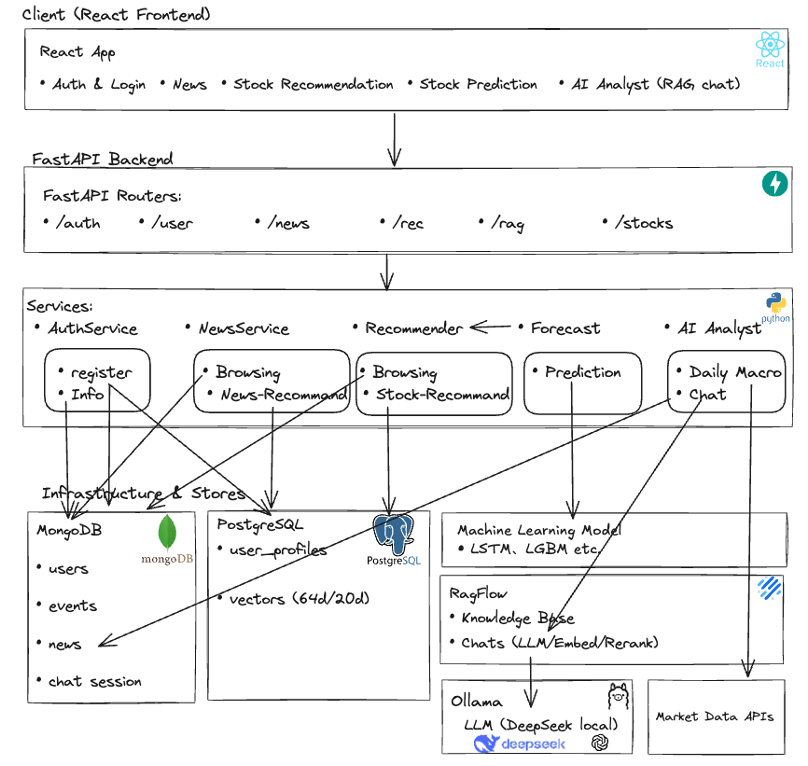
\includegraphics[width=1\linewidth]{images/system_design.png}
	\caption[system design]{Finsight system design}
	\label{fig:system_design}
\end{figure}

\subsection{System Architecture}

\begin{longtable}{p{3cm}p{10cm}}
\toprule
\textbf{Module} & \textbf{Description} \\
\midrule
News Module & Fetches financial news via Google \acs{RSS} and APIs, performs \acs{NLP} parsing and vectorization. \\
Recommendation Module & Combines user profile embeddings and stocks vectors for personalized ranking. \\
Forecast Module & Predicts stock prices using \acs{ARIMA}, Prophet, \acs{LGBM}, \acs{LSTM}, and ensemble models. \\
RAG Module & Integrates RagFlow for retrieval-augmented question answering. \\
User Profile Module & Maintains user semantic (64D) and preference (20D) embeddings and stores users base information. \\
Auth \& User Service & Handles registration, login, JWT authentication, and profile setup. \\
Database Client & Manages MongoDB, PostgreSQL, and SSH tunneling. \\
\bottomrule
\end{longtable}

\subsection{Data Flow and Integration}
\begin{enumerate}[leftmargin=1.5em]
    \item Users register for this platform. Each user will get his own user profile(a 20D vector that representsing their investment interests). Based on users' behavior(like click \ like \ dislike) to adjust their profile vector.
    \item The frontend sends a REST API request to FastAPI endpoints such as \texttt{/forecast}, \texttt{/stocks},\texttt{/news}, or \texttt{/rag}.
    \item The backend loads user profiles, news data, stock data, or knowledge base content.
    \item Depending on the task, it calls news modules, forecasting models, RAG reasoning, or recommendation logic.
    \item The backend returns structured JSON results visualized by the frontend dashboard.
\end{enumerate}

\subsection{Tech Stack}

\begin{longtable}{p{3cm}p{11cm}}
\toprule
\textbf{Layer} & \textbf{Technology and Description} \\
\midrule
Frontend & React + Vite + TailwindCSS + Recharts for interactive dashboards. \\
Backend & FastAPI (Python 3.12+) with modular routers and service layers. \\
Database & MongoDB for document data; PostgreSQL + pgvector for vector storage. \\
Machine Learning & Prophet, ARIMA, LightGBM, LSTM, Transformer and Seq2Seq forecasting. \\
LLM / RAG & RagFlow for retrieval-augmented reasoning; DeepSeek-8B and OpenAI embeddings; Ollama for llm services. \\
Infrastructure & Docker, Uvicorn, SSH tunnel, NUS \acs{HPC}, and AWS EC2 deployment. \\
\bottomrule
\end{longtable}

% \section{User Register Module}



\section{News Browsing Module}

Design goals were: a clean feed, de-duplication across sources, light personalization, and a smooth API surface. In practice we ship a two-vector design (semantic 64-d, preference 20-d), an \textbf{exclude-seen} filter backed by Mongo events, and a \textbf{dual refresh mode} that keeps first-paint fast while allowing small, quota-friendly real-time pulls. The front end renders a \(3\times 3\) grid with cached paging (previous/next/jump), so user actions immediately influence subsequent pages without blocking the UI.

\subsection{Overall Architecture Design}
The module follows a clear \textbf{Service ⟂ Repository} split with thin HTTP endpoints:

\begin{itemize}
  \item \textbf{Datastores.} News and events are stored in \textbf{MongoDB} (documents: title, url, source, \texttt{published\_at}, tickers, sector, topics, sentiment, plus 20-d profile vector \(\mathbf{p}_a\)); \textbf{PostgreSQL + pgvector} holds the normalized 64-d semantic embeddings for articles and the 20-d user profile \(\mathbf{u}\in\mathbb{R}^{20}\).
  \item \textbf{Service core (NewsService).} Orchestrates candidate gathering, scoring, and post-filters. It also coordinates a tiny ``trickle'' ingestion when \texttt{refresh=1}---pulling \(\le 3\) fresh items using symbol hints, upserting them, then re-ranking together with the local corpus.
  \item \textbf{Repositories.}
    \begin{itemize}
        \item \texttt{NewsRepo} (Mongo) for latest/news lookup and upserts.
        \item \texttt{PgProfileRepo} (Postgres) for \(\mathbf{u}\) updates and vector math.
        \item \texttt{EventRepo} (Mongo) logging \texttt{click/like/bookmark}, plus a compact \textbf{toggle} collection for idempotent ``add'' and reversible ``remove''.
    \end{itemize}
  \item \textbf{HTTP surface (FastAPI).}
    \begin{itemize}
        \item \texttt{GET /rec/user/news} -- ranked results with \texttt{refresh=\{0,1\}}, \texttt{symbols=}, \texttt{exclude\_hours=} (exclude seen).
        \item \texttt{POST /users/event/\{click|like|bookmark\}} -- log behavior and update \(\mathbf{u}\).
        \item \texttt{GET /debug/news/latest} -- fast first-paint sample (9 items) directly from the DB.
    \end{itemize}
\end{itemize}

This layout keeps hot read paths short (DB-only) while still supporting tiny real-time updates, and isolates vector math and schema evolution behind stable service methods.

\subsection{Candidates, Scoring, and Ranking}

At request time, the service constructs a candidate set and ranks it with a compact, interpretable score. If \texttt{refresh=0}, candidates are simply the latest \(K\) items from Mongo; if \texttt{refresh=1}, the service first pulls a \textbf{very small} batch of fresh articles (guided by \textbf{top-3 tickers} on the current page), upserts, and then re-queries latest. After candidate assembly we apply \textbf{exclude-seen} using recent user events (click/like/bookmark) within a sliding window (e.g., 30 days), then de-dup strictly by \texttt{news\_id}.

The final score blends preference match, recency, and page-level diversity, then clips to \([0,1]\):
\[
\mathrm{score}(u,a)\;=\;
\alpha\,\cos\!\big(\mathbf{u},\mathbf{p}_a\big)
\;+\;\beta\,f_{\text{recency}}(a)
\;+\;\gamma\,f_{\text{diversity}}(a\mid\mathcal{S})
\;\;\in[0,1].
\]
Here \(\mathbf{p}_a\in\mathbb{R}^{20}\) is the article’s 20-d preference vector aligned with our sector/bucket basis; \(f_{\text{recency}}\) mildly favors newer items; \(f_{\text{diversity}}\) discourages near-duplicates within the top-\(N\) slate \(\mathcal{S}\). We then take the top \(N=9\) for one page and return \(\{\text{title, url, source, published\_at, tickers, sector}\}\) for rendering.

\subsection{Feedback Loop and Online Profile Updates}

Interactions close the loop via \textbf{append-only events} in Mongo and immediate updates to the 20-d user profile \(\mathbf{u}\) in Postgres. Each click carries a weight:
\[
w \;=\; 1 \;+\; 0.5\,\mathbf{1}[\text{dwell}\ge 10\text{s}]
\;+\; 0.5\,\mathbf{1}[\texttt{liked}]
\;+\; 0.5\,\mathbf{1}[\texttt{bookmarked}].
\]
For \textbf{positive} actions (add) we nudge toward the article’s preferences:
\[
\mathbf{u} \;\leftarrow\; \mathbf{u} \;+\; \eta\,w\,\mathbf{p}_a.
\]
For \textbf{removals} (e.g., un-like / un-bookmark) we apply a \textbf{fixed decrement} to the same dimensions---simple, stable, and snapshot-free:
\[
\mathbf{u} \;\leftarrow\; \mathbf{u} \;-\; \eta_r\,\mathbf{p}_a,
\qquad \eta_r \ll \eta .
\]
We de-duplicate ``add'' by a \((\texttt{user}, \texttt{news}, \texttt{type})\) toggle so repeated likes do not double-count, and we no-op ``remove'' if the toggle is already off. In practice this yielded \textbf{monotone} improvements after positive feedback and sensible reversion after removals, without the fragility of storing/restoring full vector snapshots.

\subsection{Latency, Caching, and Refresh Modes}

To keep the interface responsive and protect API quotas, we maintain two coordinated modes:

\begin{itemize}
  \item \textbf{DB-only paging (\texttt{refresh=0}).} Used for initial paint and most page turns. The front end caches pages locally (arrays of 9 items) and keeps a set of \texttt{seenIds}. ``Previous'' and page jumps are pure client operations; ``Next'' is also cached unless the user is already on the \textbf{last} page.
  \item \textbf{Trickle refresh (\texttt{refresh=1}).} Triggered only when the user is on the last page and presses ``Next.'' The service pulls at most a few \textbf{fresh articles} (guided by the current page’s top-3 tickers), upserts, and re-ranks together with the corpus---delivering freshness at a \textbf{tiny} marginal cost.
\end{itemize}

In both modes, the server still enforces exclude-seen and de-dup, ensuring the \(3\times 3\) slate remains \textbf{novel}. The front end never blocks on re-ranking to show cached pages; it only waits on network when specifically expanding the tail with \texttt{refresh=1}.

\section{Stock Recommendation Module Architecture}

\subsection{Overall Architecture Design}

The stock recommendation module employs a sophisticated \textbf{microservices} architecture that seamlessly integrates with the broader investment platform. As illustrated in Figure \ref{fig:recommend_overview}, the module operates as a central intelligence hub, processing user preferences, market data, and financial metrics to generate personalized investment recommendations.

\begin{figure}[ht!] % supposedly places it here ...
	\centering
	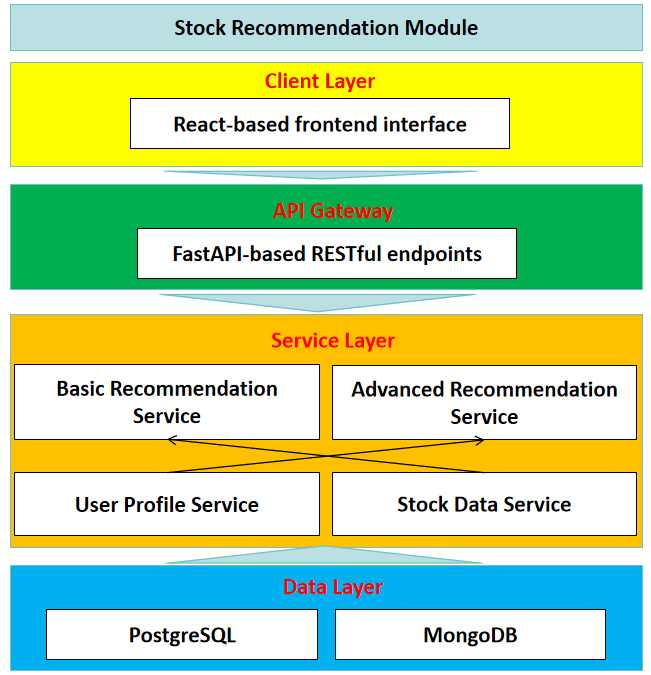
\includegraphics[scale=0.8]{images/stock_recommend/recommend_overview.png}
	\caption{Stock Recommendation System Architecture}
	\label{fig:recommend_overview}
\end{figure}


The architecture is designed for scalability and real-time performance, employing asynchronous processing patterns and intelligent caching strategies. The module supports multiple recommendation strategies that can be dynamically selected based on user preferences and market conditions.

\subsection{Basic Recommendation Engine}

The basic recommendation engine forms the \textbf{foundation} of our stock recommendation system, implementing a sophisticated vector similarity approach combined with intelligent diversification.

\textbf{Vector Similarity Foundation:}
The core algorithm computes \textbf{cosine} similarity between 20-dimensional user and stock vectors:

\begin{equation}
\text{Similarity}(\mathbf{U}, \mathbf{S}) = \frac{\sum_{i=1}^{20} U_i \cdot S_i}{\sqrt{\sum_{i=1}^{20} U_i^2} \cdot \sqrt{\sum_{i=1}^{20} S_i^2}}
\end{equation}

Where $\mathbf{U}$ represents the user's 20-dimensional preference vector and $\mathbf{S}$ represents the stock's 20-dimensional characteristic vector. The 20 dimensions are carefully engineered to capture both sector preferences (dimensions 0-10) and investment style preferences (dimensions 11-19).

\textbf{Diversification Enhancement:}
To prevent over-concentration in specific sectors, the system implements a dynamic diversification mechanism:

\begin{equation}
\text{Final Score} = \text{Raw Similarity} - \alpha \cdot \mathbb{I}_{\text{sector seen}}
\end{equation}

Where $\alpha$ is the diversity factor (configurable from 0 to 0.3) and $\mathbb{I}_{\text{sector seen}}$ is an indicator function that equals 1 if the sector has already been selected in the current recommendation batch. This approach ensures that even if multiple technology stocks have high similarity scores, the system will prioritize including stocks from underrepresented sectors.

This approach ensures that recommendations are both personalized to user preferences and strategically diversified across market sectors.

\subsection{Advanced Multi-Objective Recommendation Engine}

The advanced recommendation engine represents a significant evolution beyond basic similarity matching, implementing a sophisticated multi-objective optimization framework that balances four critical investment dimensions.

\textbf{Multi-Objective Optimization Framework:}
The final recommendation score is computed as a weighted combination of four component scores:

\begin{equation}
\text{Final Score} = w_p \cdot S_p + w_r \cdot S_r + w_d \cdot S_d + w_t \cdot S_t
\end{equation}

Each component score represents a distinct investment objective:

\textbf{Preference Similarity Score ($S_p$)}:
This component measures alignment between user preferences and stock characteristics using the same 20-dimensional vector similarity as the basic engine, but with additional normalization to ensure compatibility with other components.

\textbf{Risk-Adjusted Return Score ($S_r$)}:
This sophisticated component evaluates the risk-reward profile of each stock:

\begin{equation}
S_r = \frac{\text{Expected Return}}{\max(\text{Volatility}, 0.01)}
\end{equation}

Expected return is estimated using a multi-factor model:
\begin{equation}
\text{Expected Return} = 0.3 \cdot R_{\text{historical}} + 0.4 \cdot R_{\text{growth}} + 0.3 \cdot R_{\text{valuation}}
\end{equation}

Where:
\begin{itemize}
\item $R_{\text{historical}}$: 3-month price momentum normalized to annual returns
\item $R_{\text{growth}}$: Revenue growth projections from fundamental analysis
\item $R_{\text{valuation}}$: Valuation reversal effect based on P/E ratios
\end{itemize}

Volatility is computed from 30-day historical price movements and annualized for consistency.

\textbf{Diversification Benefit Score ($S_d$)}:
This component evaluates each stock's contribution to portfolio diversification:

\begin{equation}
S_d = 1 - \text{Sector Concentration}
\end{equation}

Sector concentration is calculated as:
\begin{equation}
\text{Sector Concentration} = \frac{\text{Number of stocks in sector}}{\text{Total stocks in universe}}
\end{equation}

This ensures that stocks from underrepresented sectors receive higher diversification scores, promoting balanced portfolio construction.

\textbf{Market Timing Score ($S_t$)}:
This dynamic component adapts recommendations to current market conditions:

\begin{equation}
S_t = \begin{cases}
\beta \cdot 0.8 + \text{Dividend Yield} \cdot 5 \cdot 0.2 & \text{if bear market} \\
\beta \cdot 0.8 + \text{Growth Score} \cdot 0.2 & \text{if bull market} \\
(1 - \text{Volatility}) \cdot 0.5 + \text{Valuation Score} \cdot 0.5 & \text{if sideways market}
\end{cases}
\end{equation}

Market regime detection analyzes SPY ETF data using 3-month returns and volatility:
\begin{itemize}
\item \textbf{Bull Market}: Return > 10\% and Volatility < 20\%
\item \textbf{Bear Market}: Return < -5\% and Volatility > 25\%
\item \textbf{Sideways Market}: All other conditions
\end{itemize}

\textbf{Dynamic Weight Adjustment:}
The system employs risk-profile-based weight configurations:

\begin{table}[h]
\centering
\caption{Multi-Objective Weight Configuration by Risk Profile}
\begin{tabular}{|l|c|c|c|c|}
\hline
\textbf{Risk Profile} & \textbf{Preference ($w_p$)} & \textbf{Risk Return ($w_r$)} & \textbf{Diversification ($w_d$)} & \textbf{Timing ($w_t$)} \\
\hline
Conservative & 0.2 & 0.4 & 0.3 & 0.1 \\
Balanced & 0.3 & 0.4 & 0.2 & 0.1 \\
Aggressive & 0.3 & 0.5 & 0.1 & 0.1 \\
\hline
\end{tabular}
\end{table}

\subsection{Real-time User Behavior Integration}

Both recommendation engines incorporate real-time user feedback to continuously refine preference models:

\begin{equation}
\mathbf{U}_{t+1} = \mathbf{U}_t + \eta \cdot (\mathbf{S} - \mathbf{U}_t)
\end{equation}

Where $\eta$ is the learning rate that varies by behavior type:
\begin{itemize}
\item $\eta = 0.05$ for click interactions
\item $\eta = 0.20$ for favorite/dislike actions
\item $\eta = -0.20$ for removal of previous interactions
\end{itemize}

This adaptive learning mechanism ensures that the system evolves with user preferences, providing increasingly relevant recommendations over time.




% ==========================================================================================
\section{Stock Trend Prediction Module}

The Stock Forecasting module forms one of the core intelligent reasoning components of the FinSight system. 
It provides users with \textbf{real-time price forecasting} capabilities powered by machine learning and time-series models.
The system integrates a FastAPI-based backend with a React-based frontend, enabling seamless interaction and visualization.

\subsection{System Architecture}

The stock prediction module forms a core component of the FinSight system, providing short-horizon predictions such as one-day, seven-day, and thirty-day forward prices.  
We demonstrate familiarity with \textbf{\acf{MLOps}} here. It adopts a microservice architecture that \textbf{separates responsibilities} between data processing, model inference, and user presentation.  
The backend, implemented in Python using the FastAPI framework, exposes several endpoints.
These endpoints handle data retrieval, model orchestration, and forecast generation.  
Historical price data are stored in MongoDB database, where each document contains time-series data represented as a list of date-close pairs.  
The forecasting service reads this data, invokes the appropriate prediction models, and returns structured results through a REST interface.

On the frontend,  
The user can select a stock ticker from the recommandation tickers' list, and the interface presents both the last seven actual closing prices and the predicted trend for upcoming horizons.  
This integration enables a smooth interaction between data analytics and visualization, delivering both reasoning and interpretability to end users.

The \textbf{Stock Trend Prediction Module Design} is shown in Figure 4.3

\begin{figure}[ht!] 
	\centering
	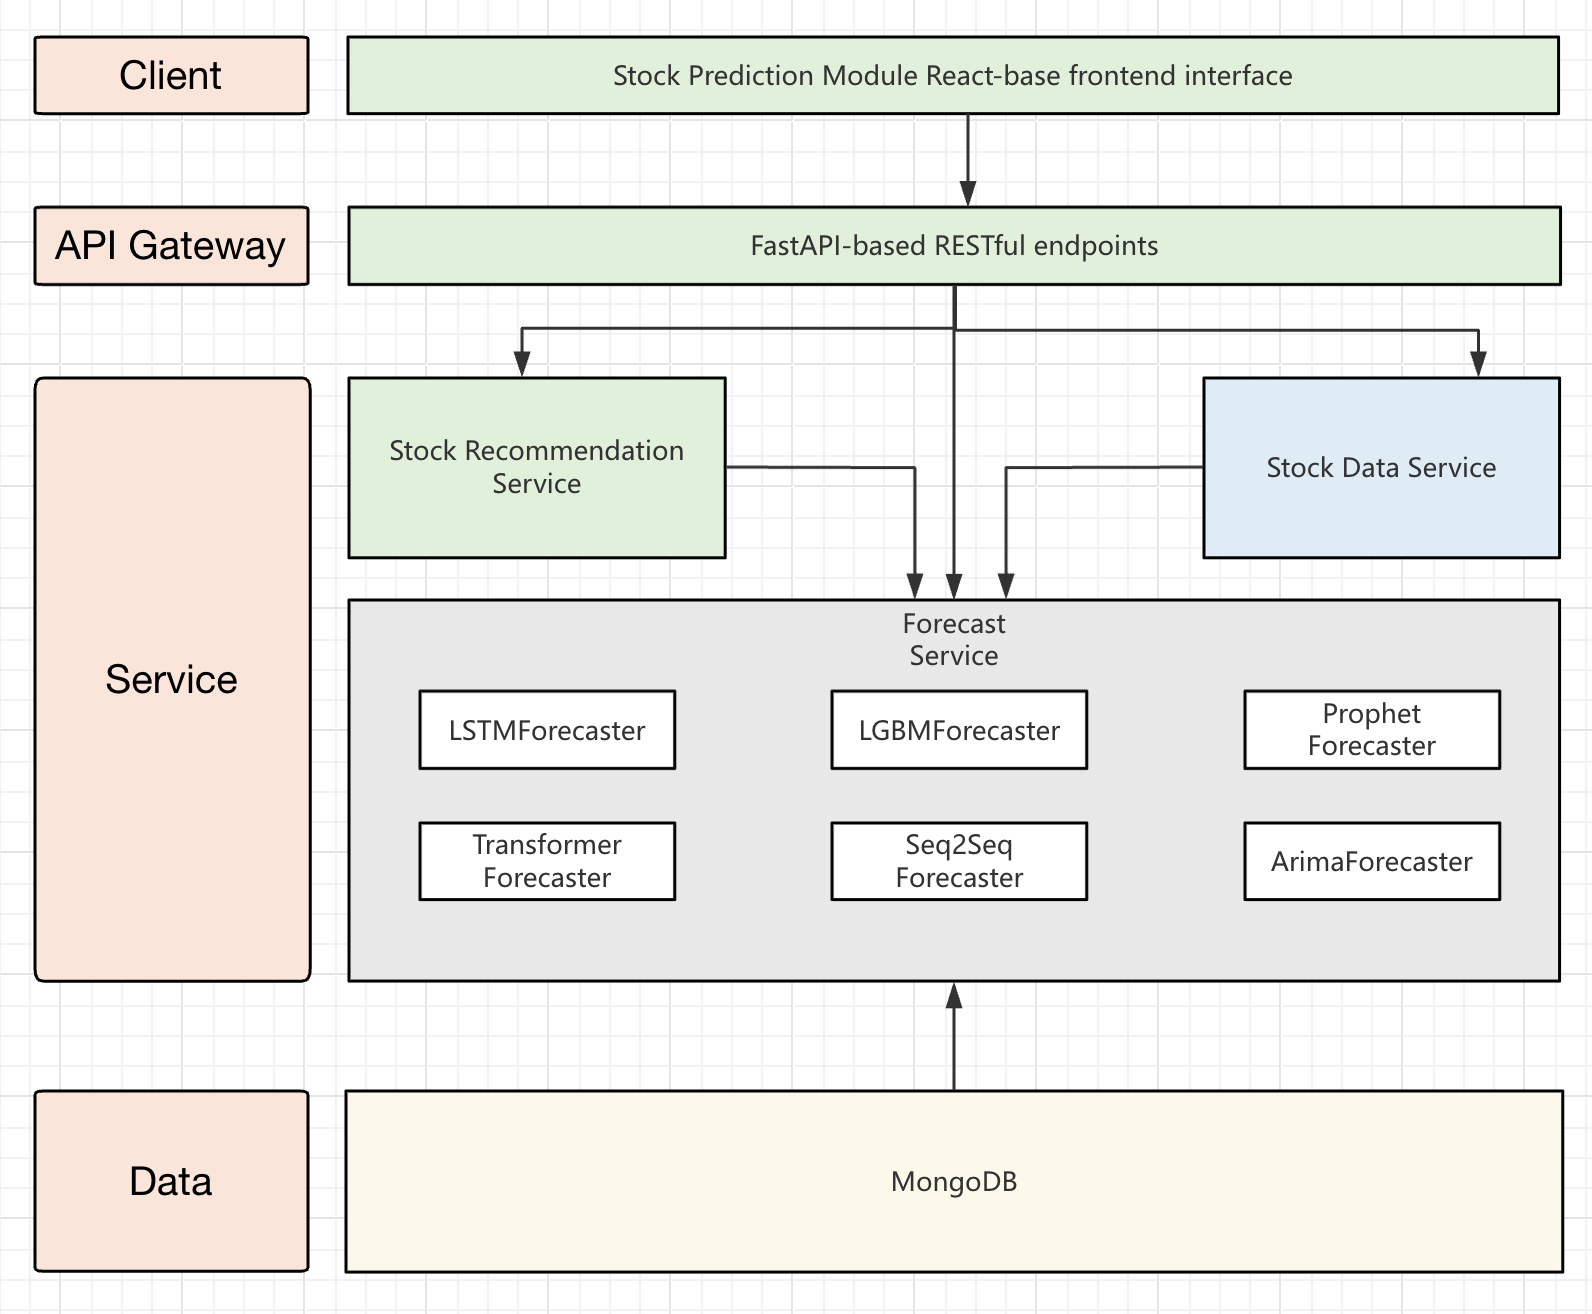
\includegraphics[width=1\linewidth]{images/prediction/arch.png}
	\caption[system design]{Stock Trend Prediction Module Design}
\end{figure}


\subsection{Frontend and Backend Data Processing}

The data flow between the frontend and backend follows a clear \textbf{five-stage} pipeline.  
\textbf{First}, the user selects a ticker symbol within the interface.  
The \textbf{frontend then} issues two asynchronous requests to retrieve the most recent seven actual closing prices.  
Upon receiving these requests, the \textbf{backend} loads the corresponding historical series from our MongoDB database, performs validation, and automatically determines which forecasting model or ensemble to use based on data length and volatility.  
The \textbf{chosen model} then produces a list of predicted values, each associated with a forecast horizon in days and optionally a confidence score.  
All results are \textbf{normalized} into a unified \texttt{ForecastResult} structure, which contains the ticker symbol, current price, model name, and an array of prediction points.

On the frontend side, the two responses are merged into a continuous timeline that combines historical and future values.  
Dates for predicted points are generated by adding the forecast horizon to the current date, ensuring chronological alignment.  
The React component then renders a dual-line chart using the Recharts library, where the solid line represents actual historical prices and the dashed line displays the predicted trajectory.  
When available, confidence intervals can also be visualized as shaded bands around the prediction curve. 

Through this bidirectional communication pipeline, users experience a real-time, interpretable forecasting workflow that blends reasoning and visualization.

\subsection{Forecaster Types and Selection}

The forecasting service integrates a diverse set of models organized into three methodological families. 

The forecasting engine integrates multiple models spanning statistical, machine learning, and deep learning approaches.  
Each model family contributes a distinct reasoning capability to handle different market conditions and data characteristics.  
A summary of these forecasters is given below:

\begin{itemize}

  \item \textbf{LSTM (Long Short-Term Memory).}
  
  LSTM is a \textbf{recurrent neural network} architecture capable of learning long-range temporal dependencies.
  It aims at mitigating the vanishing gradient problem commonly encountered by traditional RNNs.
  It excels in capturing nonlinear price dynamics and is particularly effective with large, continuous datasets.

  An LSTM unit consists of \textbf{a cell and three gates}---input, forget, and output---that regulate the flow of information.
The cell preserves information across time, while the gates determine what to discard, store, or output based on the current input and previous state.
This selective control enables the network to retain long-term dependencies and make accurate sequential predictions.

The compact form of the equations for the forward pass of an LSTM cell with a forget gate is given by:

\begin{align}
f_t &= \sigma_g(W_f x_t + U_f h_{t-1} + b_f), \\
i_t &= \sigma_g(W_i x_t + U_i h_{t-1} + b_i), \\
o_t &= \sigma_g(W_o x_t + U_o h_{t-1} + b_o), \\
\tilde{c}_t &= \sigma_c(W_c x_t + U_c h_{t-1} + b_c), \\
c_t &= f_t \odot c_{t-1} + i_t \odot \tilde{c}_t, \\
h_t &= o_t \odot \sigma_h(c_t),
\end{align}

where the initial values are \( c_0 = 0 \) and \( h_0 = 0 \), and the operator \( \odot \) denotes the element-wise product.  
The subscript \( t \) indexes the time step.

\paragraph{\textbf{Variables}}
Let superscripts \( d \) and \( h \) refer to the number of input features and hidden units, respectively:
\begin{itemize}
    \item \( x_t \in \mathbb{R}^{d} \): input vector to the LSTM unit,
    \item \( f_t \in (0,1)^{h} \): forget gate's activation vector,
    \item \( i_t \in (0,1)^{h} \): input/update gate's activation vector,
    \item \( o_t \in (0,1)^{h} \): output gate's activation vector,
    \item \( \tilde{c}_t \in (-1,1)^{h} \): cell input activation vector,
    \item \( c_t \in \mathbb{R}^{h} \): cell state vector,
    \item \( h_t \in (-1,1)^{h} \): hidden state vector (also known as the output vector),
    \item \( W \in \mathbb{R}^{h \times d}, \; U \in \mathbb{R}^{h \times h}, \; b \in \mathbb{R}^{h} \): weight matrices and bias vectors learned during training.
\end{itemize}

\paragraph{Activation \textbf{Functions}}
\begin{itemize}
    \item \( \sigma_g \): sigmoid activation function,
    \item \( \sigma_c \): hyperbolic tangent function,
    \item \( \sigma_h \): hyperbolic tangent function, or the identity function \( \sigma_h(x) = x \) in the peephole LSTM variant.
\end{itemize}


  \item \textbf{ARIMA (Auto-Regressive Integrated Moving Average).}  
  
  A classical time-series model that captures \textbf{autocorrelation patterns and local trends}.  
  It performs well for stationary or mildly non-stationary data and is computationally efficient for short horizons.
  We use non-seasonal ARIMA model in the Finsight prediction module.

\textbf{Non-seasonal} ARIMA models are usually denoted as \( \mathrm{ARIMA}(p, d, q) \), 
where the parameters \( p, d, q \) are non-negative integers.  
Here, \( p \) is the order (number of time lags) of the \textit{autoregressive} part of the model,  
\( d \) is the degree of differencing (the number of times the data have had past values subtracted),  
and \( q \) is the order of the \textit{moving-average} part.  


Given time series data \( X_t \), where \( t \) is an integer index and \( X_t \) are real numbers,  
an \( \mathrm{ARMA}(p', q) \) model is given by

\begin{equation}
X_t - \alpha_1 X_{t-1} - \cdots - \alpha_{p'} X_{t-p'} 
= \varepsilon_t + \theta_1 \varepsilon_{t-1} + \cdots + \theta_q \varepsilon_{t-q},
\end{equation}

or equivalently,

\begin{equation}
\left( 1 - \sum_{i=1}^{p'} \alpha_i L^i \right) X_t
= \left( 1 + \sum_{i=1}^{q} \theta_i L^i \right) \varepsilon_t,
\end{equation}

where \( L \) is the \textit{lag operator}, 
the \( \alpha_i \) are the parameters of the autoregressive part of the model, 
the \( \theta_i \) are the parameters of the moving average part, 
and the \( \varepsilon_t \) are the error terms.  
The error terms \( \varepsilon_t \) are generally assumed to be 
independent and identically distributed (i.i.d.) random variables 
sampled from a normal distribution with zero mean.


  \item \textbf{Transformer.}

  The Transformer forecaster adopts a \textbf{self-attention}-based architecture that replaces recurrent computation 
with parallelizable attention mechanisms.  
Unlike RNNs, which process sequences step by step, 
Transformers model all time-step relationships simultaneously, 
allowing them to learn long-range dependencies and contextual interactions more efficiently.

Given an input matrix \( X \in \mathbb{R}^{L \times d} \) of historical embeddings, 
the self-attention mechanism computes:
\begin{equation}
\mathrm{Attention}(Q, K, V) = \mathrm{softmax}\!\left(\frac{QK^{\top}}{\sqrt{d_k}}\right)V,
\end{equation}
where \( Q = XW_Q \), \( K = XW_K \), and \( V = XW_V \) 
are the query, key, and value projections with learnable matrices \( W_Q, W_K, W_V \in \mathbb{R}^{d \times d_k} \).  
This attention operation enables the model to weigh the relative importance of all past observations 
when producing a new forecast representation.

The Transformer forecaster \textbf{used in FinSight} employs multiple attention heads and residual feed-forward layers 
to capture both local and global temporal structures.  
Positional encodings are added to preserve sequence order, 
and layer normalization ensures stable convergence during training.  
The decoder projects the attention output to the predicted horizon through a linear layer.



  \item \textbf{Seq2Seq.}
  
  The Sequence-to-Sequence (Seq2Seq) forecaster extends the recurrent neural network framework by \textbf{explicitly separating the encoding and decoding} phases of temporal modeling.  
In the FinSight implementation, the encoder reads an input sequence of historical prices 
and compresses it into a latent representation \( h_t \), which summarizes the temporal dynamics of the recent window.  
The decoder then unfolds this hidden context over future horizons, generating multiple predicted values recursively or in parallel.

Formally, given an input sequence \( X = (x_{t-L+1}, \ldots, x_t) \), 
the encoder produces a sequence of hidden states:
\begin{equation}
h_j = f_{\mathrm{enc}}(x_j, h_{j-1}), \quad j = t-L+1, \ldots, t,
\end{equation}
where \( f_{\mathrm{enc}} \) is typically a \acf{GRU} or long short-term memory (LSTM) cell.  
The decoder then generates forecasted outputs \( \hat{y}_{t+k} \) as:
\begin{equation}
s_k = f_{\mathrm{dec}}(s_{k-1}, \hat{y}_{t+k-1}, h_t), \qquad
\hat{y}_{t+k} = W_o s_k + b_o,
\end{equation}
where \( s_k \) is the decoder hidden state and \( h_t \) provides context from the encoder.

The Seq2Seq design allows the model to capture asymmetric temporal dependencies between past and future horizons.  
It can learn patterns where the relevance of earlier observations decays non-linearly, and can adapt to varying forecast lengths without retraining.  
In FinSight, this forecaster is implemented as a lightweight, single-layer \acs{GRU}-based encoder decoder pair, optimized for short- to medium-term forecasting horizons.  
The model selection policy \textbf{activates} the Seq2Seq forecaster when the \textbf{available training series is sufficiently long} 
and exhibits \textbf{sequential dependencies} that simpler autoregressive models cannot capture effectively.
  

  \item \textbf{Prophet.}  
  
  Prophet is a procedure for forecasting time series data based on an \textbf{additive model} where non-linear trends are fit with yearly, weekly, and daily seasonality, plus holiday effects. It works best with time series that have \textbf{strong seasonal effects and several buckets of historical data}. Prophet is robust to missing data and shifts in the trend, and typically handles outliers well.

  \item \textbf{LightGBM(Light Gradient-Boosting Machine).}  
  
  A gradient boosting framework based on \textbf{decision trees} that can model nonlinear relationships and interactions. It is used for ranking, classification and other machine learning tasks.
  When using gradient descent, one thinks about the space of \textbf{possible configurations of the model as a valley}, in which the lowest part of the valley is the model which most closely fits the data. In this metaphor, one walks in different directions to learn how much lower the valley becomes.
  When enhanced with engineered lag and technical indicators, it yields highly adaptive short-term forecasts.


\end{itemize}



Together, these components form a cohesive reasoning system that bridges data analytics with cognitive visualization.  

It showcases an intelligent forecasting pipeline capable of autonomous model choice, explainable prediction generation, and visually intuitive results that facilitate informed financial decision-making.

% =====================================================================================
\section{AI Analyst}

\subsection{System Overview}

The FinSight AI Analyst subsystem enables both daily macro data checking and financial question answering by combining Large Language Models (LLMs) with a retrieval-based knowledge engine (RagFlow).


\paragraph{\textbf{Core Objectives}}

\begin{enumerate}
	\item Integrate retrieval and reasoning to produce accurate, evidence-backed answers specific in Finance Field.
	\item Enable multi-turn dialogue with persistent contextual memory.
	\item Allow dynamic selection of model and knowledge base per user query.
	\item Maintain modular, extensible backend architecture.
\end{enumerate}

\subsection{Architecture}
\begin{figure}[t]
  \centering
  \begin{adjustbox}{width=\textwidth,max height=0.95\textheight}
  \begin{tikzpicture}[
    node distance=10mm and 14mm,
    >={Latex[length=2mm]},
    tiny/.style={font=\tiny},
    box/.style={rounded corners=2pt,draw,fill=white,align=center,inner sep=3pt,
                minimum width=28mm,minimum height=7mm},
    wide/.style={rounded corners=2pt,draw,fill=white,align=center,inner sep=3pt,
                 minimum width=56mm,minimum height=8mm},
    group/.style={dash pattern=on 2pt off 2pt,rounded corners=3pt,draw=gray!60,inner sep=8pt},
    grouplabel/.style={font=\tiny\bfseries,fill=white,inner sep=2pt}
  ]

  % ===== Ingestion =====
  \node[box,tiny] (news)    {News/APIs};
  \node[box,tiny,right=of news] (filings) {Filings\\(EDGAR/SGX)};
  \node[box,tiny,right=of filings] (uploads) {User Docs};

  % ===== Parse / Embed stack =====
  \node[wide,tiny,below=13mm of $(news)!0.5!(uploads)$] (extract)
     {Extract / Parse\\ \scriptsize Trafilatura (web) | Unstructured (files)};
  \node[wide,tiny,below=of extract] (chunk)
     {Chunk \& Normalize\\ \scriptsize overlap + metadata (URL, doc, page)};
  \node[wide,tiny,below=of chunk] (embed)
     {Embeddings\\ \scriptsize BGE/E5 encoders};

  \draw[->] (news) -- (extract);
  \draw[->] (filings) -- (extract);
  \draw[->] (uploads) -- (extract);
  \draw[->] (extract) -- (chunk);
  \draw[->] (chunk) -- (embed);

  % ===== Vector Stores (wider spacing) =====
  \coordinate (vecbase) at ($(embed) + (0,-20mm)$);
  \node[box,tiny] (uvec) at ($(vecbase)+(-48mm,0)$) {User\\Vectors};
  \node[box,tiny] (nvec) at ($(vecbase)+(-16mm,0)$) {News\\Vectors};
  \node[box,tiny] (svec) at ($(vecbase)+(16mm,0)$)  {Ticker\\Vectors};
  \node[box,tiny] (retr) at ($(vecbase)+(48mm,0)$)  {LLM Retriever\\Index};

  % Embed -> vectors: 4 arrows from embed, through junction, to each vector store
  \coordinate (embedjunction) at ($(embed.south) + (0,-5mm)$);
  \draw[->,rounded corners=3pt] (embed.south) -- (embedjunction) -| (uvec.north);
  \draw[->,rounded corners=3pt] (embed.south) -- (embedjunction) -| (nvec.north);
  \draw[->,rounded corners=3pt] (embed.south) -- (embedjunction) -| (svec.north);
  \draw[->,rounded corners=3pt] (embed.south) -- (embedjunction) -| (retr.north);

  % ===== Signals (left side column with more space) =====
  \coordinate (sigcol) at ($(uvec) + (-42mm,0)$);
  \node[box,tiny] (risk) at ($(sigcol)+(0, 13mm)$) {Risk Lens\\ \scriptsize vol/beta};
  \node[box,tiny] (sent) at ($(sigcol)+(0,  0mm)$) {Finance\\Sentiment\\ \scriptsize FinBERT};
  \node[box,tiny] (fcst) at ($(sigcol)+(0,-13mm)$) {Forecasting\\ \scriptsize LSTM/Xformers};

  % Signal connections with curved arrows (fluid routing)
  \draw[->,rounded corners=3pt] (uvec.west) to[out=180,in=0] (risk.east);
  \draw[->,rounded corners=3pt] (nvec.south west) to[out=220,in=0] (sent.east);
  \draw[->,rounded corners=3pt] (svec.south west) to[out=240,in=0] (fcst.east);

  % ===== Retrieve & Rerank =====
  % Define a consolidation point for all vector inputs
  \coordinate (consolidation) at ($(vecbase) + (0,-20mm)$);
  
  \node[wide,tiny,below=20mm of $(nvec)!0.5!(svec)$] (ann)
    {ANN Retrieval (cosine/IP)\\ \scriptsize FAISS (HPC) | pgvector (Postgres)};
  \node[box,tiny,right=16mm of ann] (rerank)
    {Cross-Encoder\\Reranker\\ \scriptsize bge-reranker-v2-m3};

  % All four vector stores converge to single point on ANN box
  \draw[->,rounded corners=3pt] (uvec.south) -- ++(0,-8mm) -| (consolidation) -- (ann.north);
  \draw[->,rounded corners=3pt] (nvec.south) -- ++(0,-5mm) -| (consolidation);
  \draw[->,rounded corners=3pt] (svec.south) -- ++(0,-5mm) -| (consolidation);
  \draw[->,rounded corners=3pt] (retr.south) -- ++(0,-8mm) -| (consolidation);
  
  \draw[->] (ann) -- (rerank);

  % ===== RAG + Serving =====
  \node[wide,tiny,below=13mm of $(ann)!0.5!(rerank)$] (rag)
    {RAG Layer\\ \scriptsize FastAPI (custom) | RAGFlow (orchestration)};
  \draw[->] (rerank.south) -- (rag.north);

  \node[wide,tiny,below=of rag] (llm)
    {LLM Server\\ \scriptsize vLLM (OpenAI-compatible) | Ollama/DeepSeek};
  \draw[->] (rag) -- (llm);

  % ===== Outputs =====
  \node[box,tiny,below left=13mm and 8mm of llm] (answers)
    {Analyst-style\\Answers\\ \scriptsize reasoning +\\citations};
  \node[box,tiny,below right=13mm and 8mm of llm] (feeds)
    {News/\\Watchlists\\ \scriptsize "what changed"\\+ tags};

  % Both output arrows: 2 arrows from llm, through junction, to each output box
  \coordinate (llmout) at ($(llm.south) + (0,-5mm)$);
  \draw[->,rounded corners=3pt] (llm.south) -- (llmout) -| (answers.north);
  \draw[->,rounded corners=3pt] (llm.south) -- (llmout) -| (feeds.north);

  % ===== GROUPS (behind, with labels on right side) =====
  \begin{scope}[on background layer]
    \node[group,fit=(news)(filings)(uploads)] (ing) {};
    \node[grouplabel,anchor=south,yshift=3mm] at (ing.north) {Ingestion};
    
    \node[group,fit=(extract)(chunk)(embed)] (parse) {};
    \node[grouplabel,anchor=west] at (parse.east) {Parsing \& Embedding};
    
    \node[group,fit=(uvec)(nvec)(svec)(retr)] (vec) {};
    \node[grouplabel,anchor=west] at (vec.east) {Vector Stores};
    
    \node[group,fit=(risk)(sent)(fcst)] (sig) {};
    \node[grouplabel,anchor=south] at (sig.north) {Signals};
    
    \node[group,fit=(ann)(rerank)] (ret) {};
    \node[grouplabel,anchor=west] at (ret.east) {Retrieve \& Rerank};
    
    \node[group,fit=(rag)(llm)(answers)(feeds)] (gen) {};
    \node[grouplabel,anchor=north east,xshift=-2mm,yshift=-2mm] at (gen.north east) {Generation/Serving};
  \end{scope}

  \end{tikzpicture}
  \end{adjustbox}
  \caption{FinSight overview: ingest $\rightarrow$ parse $\rightarrow$ embed $\rightarrow$ retrieve \& rerank $\rightarrow$ generate.
  Vector search is the backbone (FAISS on HPC; pgvector for persistent Postgres-backed search). Sidecars provide sentiment, risk and
  short-horizon forecasts. For RAG, retrieval is reranked, then fed to an LLM server---OpenAI-compatible vLLM or Ollama/DeepSeek
  behind RAGFlow---for grounded answers with citations.}
  \label{fig:finsight-overview}
\end{figure}

AI Analyst is consisted with four modules which are Frontend $|$ Backend $|$ RagFlow $|$ Storage. The frontend is React-based web interface for user interaction. It provides input box, model/dataset selection, and chat display and displays citations and retrieved document summaries. The Backend is built for managing \textbf{session creation, context assembly, and RagFlow API calls}. It contains dedicated routers and services for modular functionality:
\begin{enumerate}
	\item /rag/chat: Handles chat requests and message orchestration.
	\item /rag/history/{id}: Retrieves chat history by session ID.
	\item /rag/models: Lists available LLM models.
	\item /rag/datasets: Lists available knowledge bases.
\end{enumerate}

% The chat task workflow is shown below:

% \begin{figure}
%     \centering
%     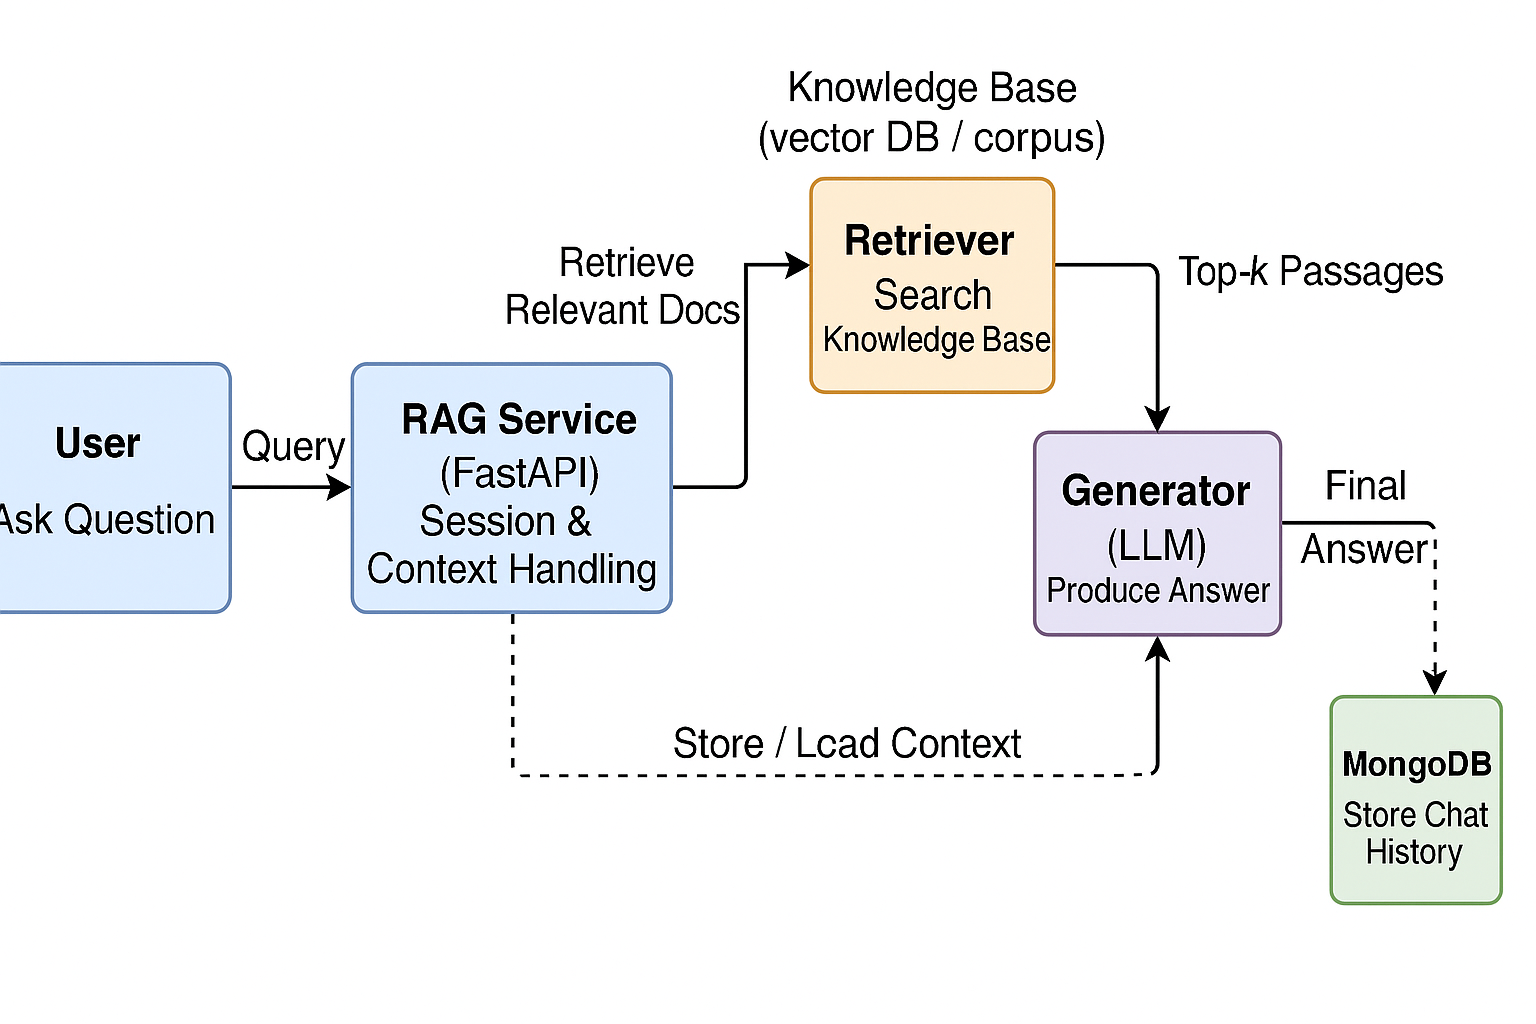
\includegraphics[width=0.75\linewidth]{images/AI_system_design.png}
%     \caption{Chat Task Workflow}
%     \label{fig:placeholder}
% \end{figure}

\textbf{RagFlow} is an external service handling document retrieval, reranking, and context-grounded generation and it exposes /api/v1/chats and OpenAI-compatible completion endpoints. Ragflow is easily deployed by \textbf{docker} and easy to use. All the chatting sessions are stored in MongoDB. It stores chat sessions, message history, and timestamps which makes Multi-round conversation available. It also supports querying, session resumption, and lightweight analytics.

% \section{Combined Investment Recommendation Module}

% This module will form a core part of our application. It will function as a semi-automated/AI-augmented Financial Research analyst (FRA). A FRA is a sector-specific or stock-specific expert who goes deep into their area/stock of expertise and tries to analyse how the sector or company will perform in the short-term and mid-term future. Their reports help investors make decisions.

% The main aim of our “Combined Investment Recommendation Module”, hereafter “CIRM” is to give all its research on any stock or any sector based on publicly available data like company reports, past experience, and domain knowledge, news, etc. We will then compare it with other analysts’ predictions to see how it has performed and to improve it. The module should also be able to revise its prediction based on news. “Combined” refers to quantitative + qualitative, multiple data sources, etc.

% In brief, Its purpose is to analyze stocks or sectors listed on Indian exchanges (NSE / BSE), aggregate data sources, run quantitative and qualitative analysis, and produce strategic reports and investment‐recommendations (risk/return / scenarios) that are transparent, defensible, and updatable.

% Our goal will be enabling an LLM in performing sentiment analysis and extracting signals from unstructured data like earnings calls, market news, and corporate filings.
% This section explains how the CIRM will be structured (conceptually), the modules, workflows, and how things connect, in a high-level way without overpromising.

% \begin{enumerate}
% 	\item Module architecture
%             \begin{itemize}
%                 \item[·] Analytics & Metrics Module: compute quantitative metrics, risk metrics, scenario modelling.
%                 \item[·] Qualitative / Text Analysis Module: process news, disclosures, risks, sentiment; extract risk factors, regulatory events.
%                 \item[·] Decision / Recommendation Module: integrates quantitative & qualitative insights, produces structured output.
%                 \item[·] Reporting & Visualization Module: generate reports with data, charts, assumptions, confidence levels.
%             \end{itemize}
% 	\item Workflow
%             \begin{itemize}
%                 \item[·] Regular update cycle (say, quarterly + event-driven): Pull in new filings, market data, sector / regulatory updates.
%                 \item[·] Triggered analyses when major events: earnings release, regulatory announcement, large price move, etc.
%                 \item[·] Peer benchmarking and scenario generation.
%             \end{itemize}
% 	\item User / Stakeholder Interface
%             \begin{itemize}
%                 \item[·] Analysts can view raw data, metrics, tweak assumptions).
%                 \item[·] Reports accessible by management / clients.
%             \end{itemize}
% 	\item Regulatory / Compliance Considerations (India / SEBI)
%             \begin{itemize}
%                 \item[·] Use only public / legally disclosed information.
%                 \item[·] Be cautious about forward-looking statements; label assumptions.
%                 \item[·] For PMS / advisory services ensure disclosures of risk, past returns, disclaimers.
%                 \item[·] Data privacy / corporate governance must be respected.
%             \end{itemize}
% \end{enumerate}















	%%	\part{Your Second Part}
    \chapter{Implementation Detail}

\section{News Browsing Module}

This section details how the news module was built to realize the system design: a two vector recommender (64-d semantic, 20-d preference) with exclude-seen filtering, dual refresh, and low-latency APIs. We focus on concrete engineering choices—ingestion, storage schemas, scoring, profile updates, paging/cache behavior, and observability—so the reader can reproduce the system end-to-end.

\subsection{API Design and Implementation}

The News Browsing Module is implemented through a structured set of RESTful API endpoints using the FastAPI framework, aligning directly with the modular architecture described earlier. Each endpoint is linked to a dedicated router function, backed by a clear service–repository abstraction that isolates business logic from database operations.

\textbf{Core API Endpoints and Functionalities:}

\begin{table}[h]
\centering
\caption{News Browsing API Endpoints Overview}
\begin{tabular}{|p{4cm}|p{2.5cm}|p{3.5cm}|p{4cm}|}
\hline
\textbf{API Endpoint} & \textbf{Method} & \textbf{Parameters} & \textbf{Implementation Details} \\
\hline
/rec/user/news & GET & user\_id, limit, refresh, exclude\_hours, symbols & Retrieve personalized ranked news; supports \texttt{refresh=\{0,1\}} dual-mode fetching \\
\hline
/users/event/\{click|like|bookmark\} & POST & user\_id, news\_id, op & Log user interactions, update 20-d user profile vector incrementally \\
\hline
/debug/news/latest & GET & None & Fetch the latest 9 stored news entries for initial UI rendering \\
\hline
/news/fetch-batch & POST & watchlist, window, source & Trigger batch ingestion from Google RSS and Marketaux APIs \\
\hline
\end{tabular}
\end{table}

The module exposes lightweight endpoints optimized for fast response times and minimal latency. For instance, \texttt{/rec/user/news} handles both cached database retrieval (\texttt{refresh=0}) and live update mode (\texttt{refresh=1}), while the \texttt{/users/event} endpoints synchronize user feedback with immediate vector updates in PostgreSQL. Each endpoint follows consistent patterns of schema validation, logging, and structured JSON response generation.

\subsection{Ingestion, Normalization, and Storage}

The pipeline is implemented as a disciplined loop
\[
\text{fetch}\;\rightarrow\;\text{normalize}\;\rightarrow\;\text{deduplicate}\;\rightarrow\;\text{enrich}\;\rightarrow\;\text{vectorize}\;\rightarrow\;\text{store}.
\]
\textbf{Sources} consist of Google RSS (broad, fast-moving headlines) and Marketaux API (finance-focused, ticker-aware feed). Each item is canonically keyed by \(\{\texttt{url}, \texttt{external\_id}\}\) to avoid duplicates across sources. Normalization trims titles, resolves redirects, strips boilerplate, and harmonizes timestamps to UTC.

\textbf{Storage split.} Enriched news documents are written into \textbf{MongoDB} (\texttt{NewsRepo}) with fields:
\[
d=\{\texttt{news\_id},\texttt{title},\texttt{url},\texttt{source},\texttt{published\_at},\texttt{tickers},\texttt{sector},\texttt{topics},\mathbf{e}_{64},\mathbf{p}_{20}\}.
\]
User profiles live in \textbf{PostgreSQL + pgvector} (\texttt{PgProfileRepo}). We maintain:
\begin{itemize}
  \item Two semantic tracks: \(\texttt{user\_semantic\_64d\_short}\) and \(\texttt{user\_semantic\_64d\_long}\in\mathbb{R}^{64}\) (EMA with different half-lives).
  \item A human-interpretable preference vector \(\mathbf{u}\in\mathbb{R}^{20}\) aligned to 11 sector + 9 investment-style dimensions. For compatibility and ease of evolution, we store a JSON-mirrored copy as \(\texttt{profile\_vector\_20d}::\texttt{TEXT}\) and component JSONs \(\texttt{industry\_preferences}, \texttt{investment\_preferences}\) (both \texttt{JSON}). Reads/writes normalize to a fixed-length 20-d list to avoid schema drift.
\end{itemize}
Append-only user events (\texttt{click/like/bookmark}) are recorded in Mongo (\texttt{EventRepo}); a small \texttt{user\_event\_toggles} collection supports idempotent add/remove for UI toggles.

\subsection{Ranking Path (\texttt{/rec/user/news}) and Exclude-Seen}

The recommendation endpoint constructs a candidate slate and ranks it with a compact score. For database-only mode (\(\texttt{refresh}=0\)), candidates are pulled from Mongo by \(\texttt{latest}(K)\). If the client is on the last page and requests \(\texttt{refresh}=1\), the service performs a \emph{trickle refresh}: fetches \(\le 3\) fresh items from Marketaux (optionally guided by the page’s \emph{top-3 tickers}), upserts, then re-queries latest. Recently interacted items are filtered out using a sliding-window set from \texttt{EventRepo}:
\[
\mathcal{C}' \;=\; \{a\in\mathcal{C}\mid a.\texttt{news\_id}\notin \texttt{seenIds}(u;\Delta T)\}.
\]
Scoring blends preference match, mild recency, and slate-level diversity:
\[
s(u,a)=\alpha\,\cos(\mathbf{u},\mathbf{p}_{20}(a))\;+\;\beta\,f_{\text{recency}}(a)\;+\;\gamma\,f_{\text{div}}(a\mid\mathcal{S}),
\quad s\in[0,1].
\]
We truncate to \(N=9\) for a single page. The endpoint returns a thin JSON for UI: \(\{\texttt{title},\texttt{url},\texttt{source},\texttt{published\_at},\texttt{tickers},\texttt{sector},\texttt{score}\}\).

\subsection{Online Profile Updates and Event Handling}

The feedback loop is closed by three endpoints: \texttt{/users/event/click}, \texttt{/users/event/like}, \texttt{/users/event/bookmark}. Clicks log dwell time and optionally carry \(\texttt{liked}/\texttt{bookmarked}\) flags; likes and bookmarks are toggleable (add/remove) with idempotency enforced in Mongo. Profile updates happen synchronously in Postgres:

\paragraph{Click-driven semantic EMA.}
Let \(\mathbf{e}_{64}(a)\) be article embedding and \(w\) the event weight
\[
w \;=\; 1 \;+\; 0.5\,\mathbf{1}[\text{dwell}\ge 10\text{s}] \;+\; 0.5\,\mathbf{1}[\text{liked}] \;+\; 0.5\,\mathbf{1}[\text{bookmarked}].
\]
We apply per-track EMA after L2-normalization:
\[
\mathbf{u}^{(\text{short})}\!\leftarrow (1-\eta_s)\mathbf{u}^{(\text{short})} + \eta_s\,w\,\widehat{\mathbf{e}}_{64}(a),\quad
\mathbf{u}^{(\text{long})}\!\leftarrow (1-\eta_\ell)\mathbf{u}^{(\text{long})} + \eta_\ell\,w\,\widehat{\mathbf{e}}_{64}(a).
\]

\paragraph{Preference (20-d) updates.}
For positive actions (\texttt{add}) we nudge toward the article’s \(\mathbf{p}_{20}(a)\) with small learning rates on two segments (sector 11-d and style 9-d), using EMA on the actually-hit dimensions; for removals (\texttt{remove}) we apply fixed decrements \((\delta_{\text{ind}},\delta_{\text{inv}})\) only on the dimensions the article meaningfully activated. All writes re-serialize to a canonical 20-d JSON string (\texttt{profile\_vector\_20d}) and update the component JSONs. This design avoids snapshot brittleness while guaranteeing the stored shape of \(\mathbf{u}\) remains a dense 20-d list.

\subsection{Caching, Refresh, and Front-End Integration}

The client-side rendering follows a paginated layout (\(3\times3\) grid) managed by React. Pages are cached locally in browser memory, and navigation among cached pages (\texttt{previous/next/jump}) does not trigger network calls. The backend only refreshes content when:
\[
\text{user\_on\_last\_page} \;\land\; \text{next\_clicked} \;\Rightarrow\; \texttt{refresh}=1.
\]
In that case, the server fetches at most 3 fresh items, upserts them into MongoDB, re-ranks the corpus, and returns the updated slate. This “dual refresh mode” guarantees minimal latency (\(<200\) ms typical) and conforms to API quota limits.  

The front end also integrates lightweight event listeners for each interaction type:
\begin{itemize}
  \item \texttt{onClick}: logs click duration and news ID.
  \item \texttt{onLike / onBookmark}: toggles user preferences visually and asynchronously triggers backend updates.
\end{itemize}
This pipeline completes a full feedback loop where user behavior directly refines recommendation results without blocking the UI.  

Overall, the implementation harmonizes real-time responsiveness with model interpretability—achieving low-latency news personalization consistent with the architectural design goals.


\section{Stock Recommendation Module Implementation}

\subsection{API Design and Implementation}

The stock recommendation module implements a comprehensive RESTful API based on FastAPI framework. The API endpoints are organized in dedicated router files and follow consistent patterns for request handling, validation, and response formatting.

\textbf{Core API Endpoints and Functionality:}

\begin{table}[h]
\centering
\caption{Stock Recommendation API Endpoints Overview}
\begin{tabular}{|p{3.5cm}|p{2.5cm}|p{3cm}|p{4cm}|}
\hline
\textbf{API Endpoint} & \textbf{Method} & \textbf{Parameters} & \textbf{Implementation Approach} \\
\hline
/stocks/recommend & GET & user\_id, top\_k, diversity\_factor & Basic recommendation using cosine similarity with sector diversification \\
\hline
/stocks/recommend/v2 & GET & user\_id, top\_k, risk\_profile & Multi-objective optimization with parallel component scoring \\
\hline
/stocks/raw-data/\{symbol\} & GET & symbol & Direct MongoDB document retrieval with data cleaning \\
\hline
/stocks/fetch-raw-data & POST & symbols & Batch yfinance data fetching with MongoDB storage \\
\hline
/stocks/update-vectors & POST & symbols & 20D vector computation and PostgreSQL update \\
\hline
/users/behavior/update & POST & user\_id, behavior\_type, stock\_symbol & Real-time user preference adjustment \\
\hline
\end{tabular}
\end{table}



\subsection{Basic Recommendation Algorithm Implementation}

The basic recommendation algorithm implements a sequential workflow focused on vector similarity with intelligent diversification. The complete implementation flow is illustrated in Figure \ref{fig:basic_implementation_flow}.

\begin{figure}[h]
\centering
\textbf{[Basic Recommendation Implementation Flowchart Description]}
\fbox{
\begin{minipage}{0.9\textwidth}
\begin{enumerate}
\setlength\itemsep{0.5em}
\item \textbf{Input Processing}: Receive user ID, top-K count, and diversity factor parameters
\item \textbf{Data Retrieval}: Fetch user vector from user\_profiles table and all stock vectors from stock\_vectors table in PostgreSQL
\item \textbf{Similarity Computation}: Calculate cosine similarity between user vector and each stock vector using scikit-learn's cosine\_similarity function
\item \textbf{Initial Ranking}: Sort all stocks by raw similarity scores in descending order
\item \textbf{Diversification Processing}: 
  \begin{itemize}
  \item Initialize empty selected stocks list and sectors seen set
  \item For each stock in sorted order:
    \begin{itemize}
    \item Apply sector penalty if sector already in sectors seen set
    \item Calculate final score: raw similarity - (diversity factor × sector penalty)
    \item Add stock to selected list and sector to sectors seen set
    \end{itemize}
  \item Stop when selected list reaches top-K size
  \end{itemize}
\item \textbf{Result Generation}: Format recommendations with symbols, names, sectors, and both raw/adjusted similarity scores
\item \textbf{API Response}: Return structured JSON response to client
\end{enumerate}
\end{minipage}
}
\caption{Basic Recommendation Algorithm Implementation Flow}
\label{fig:basic_implementation_flow}
\end{figure}

The algorithm begins by retrieving the user's 20-dimensional preference vector from the user\_profiles table alongside all available stock vectors from the stock\_vectors table in PostgreSQL. These vectors are pre-computed and encapsulate both sector characteristics and investment style preferences.

The core computation involves calculating cosine similarity between the user vector and each stock vector using scikit-learn's optimized linear algebra routines. This produces raw similarity scores representing the fundamental alignment between user preferences and stock characteristics. The stocks are then sorted by these raw scores in descending order.

The diversification mechanism represents the algorithm's key innovation. Rather than simply selecting the top-K highest similarity stocks, the system maintains a running set of selected sectors and applies configurable penalties to stocks from already-represented sectors. The diversification factor parameter (typically 0.1) controls the penalty magnitude, balancing pure similarity against sector diversity. This ensures the final recommendations provide exposure across multiple industries while maintaining high relevance to user preferences.

The complete implementation resides in the StockService.recommend\_stocks() method, with the diversification logic encapsulated in the \_diversify\_recommendations() helper method. The algorithm is optimized for low-latency responses, typically completing within 100-200 milliseconds for standard stock universes, making it suitable for real-time recommendation scenarios.

\subsection{Advanced Multi-Objective Recommendation Implementation}

The advanced recommendation algorithm implements a sophisticated parallel processing pipeline that balances four distinct investment objectives through weighted optimization. The complete implementation architecture is illustrated in Figure \ref{fig:advanced_implementation_flow}.

\begin{figure}[h]
\centering
\textbf{[Advanced Recommendation Implementation Flowchart Description]}
\fbox{
\begin{minipage}{0.9\textwidth}
\begin{enumerate}
\setlength\itemsep{0.5em}
\item \textbf{Parameter Processing}: Receive user ID, top-K count, and risk profile parameters
\item \textbf{Parallel Data Acquisition}:
  \begin{itemize}
  \item Fetch user vector from PostgreSQL
  \item Retrieve all stock vectors from PostgreSQL
  \item Batch fetch raw stock data from MongoDB
  \item Analyze current market regime using SPY ETF data
  \end{itemize}
\item \textbf{Concurrent Component Scoring}:
  \begin{itemize}
  \item \textbf{Preference Similarity}: Cosine similarity between user and stock vectors
  \item \textbf{Risk-Adjusted Return}: Expected return / volatility calculations
  \item \textbf{Diversification Benefit}: 1 - sector concentration analysis
  \item \textbf{Market Timing}: Regime-adaptive scoring based on current market conditions
  \end{itemize}
\item \textbf{Weight Application}: Apply risk-profile-specific weights to each component score
\item \textbf{Composite Scoring}: Calculate final scores using weighted sum of components
\item \textbf{Explanation Generation}: Create detailed rationales for each recommendation
\item \textbf{Result Delivery}: Return ranked recommendations with comprehensive scoring breakdown
\end{enumerate}
\end{minipage}
}
\caption{Advanced Recommendation Algorithm Implementation Flow}
\label{fig:advanced_implementation_flow}
\end{figure}

The advanced algorithm begins with parallel data acquisition, simultaneously fetching multiple data sources to minimize latency. This includes retrieving the user vector and stock vectors from PostgreSQL, batch-fetching raw stock data from MongoDB for fundamental analysis, and analyzing current market regime conditions using \acf{SPY ETF} data through yfinance integration.

The core innovation lies in the \textbf{concurrent computation of} four objective components. The \textbf{preference similarity} component calculates alignment between user and stock vectors using cosine similarity, identical to the basic algorithm. Simultaneously, the \textbf{risk-adjusted return component} computes expected returns based on historical performance, growth projections, and valuation metrics, then normalizes by volatility to produce Sharpe ratio-inspired scores.

The \textbf{diversification benefit} scoring analyzes sector concentration across the entire stock universe, assigning higher scores to stocks from underrepresented sectors to promote portfolio balance. Concurrently, the \textbf{market timing} component evaluates how well each stock aligns with the current market regime, favoring high-beta growth stocks in bull markets and defensive dividend stocks in bear markets.

After all component scores are computed, the system applies \textbf{dynamic weights} based on the user's specified risk profile. Conservative profiles (weights: 0.2 preference, 0.4 risk return, 0.3 diversification, 0.1 timing) emphasize safety and balance, while aggressive profiles (weights: 0.3 preference, 0.5 risk return, 0.1 diversification, 0.1 timing) prioritize returns and growth potential.

The weighted combination produces final scores that balance multiple investment considerations, followed by explanation generation that synthesizes component scores into human-readable rationales. This entire parallel workflow is implemented in the MultiObjectiveRecommender.recommend\_stocks() method and typically completes within 300-500 milliseconds, providing comprehensive multi-factor analysis while maintaining responsive performance.

Both algorithms integrate with the user behavior tracking system through the /users/behavior/update API endpoint, allowing real-time preference updates based on user interactions. This creates an adaptive feedback loop where user engagement continuously refines the underlying preference vectors, creating increasingly personalized investment guidance over time.
% ==========================================================================================
\section{Stock Trend Prediction Module}

\subsection{API Design and Implementation}

The stock forecasting module provides time\–series\–based prediction capabilities through a structured FastAPI service layer. Each endpoint encapsulates model orchestration, data retrieval, and standardized response formatting to ensure consistency across forecasting algorithms.

\textbf{Core API Endpoints and Functionality:}

\begin{table}[h]
\centering
\caption{Stock Forecast API Endpoints Overview}
\begin{tabular}{|p{4cm}|p{2.5cm}|p{3cm}|p{4cm}|}
\hline
\textbf{API Endpoint} & \textbf{Method} & \textbf{Parameters} & \textbf{Implementation Approach} \\
\hline
/forecast/\{ticker\} & GET & ticker, horizons, method & Main entry point for model-based forecasting (ARIMA / Prophet / LGBM / LSTM) \\
\hline
/forecast/batch & GET & limit, method, ticker & Batched multi-stock forecasting for dashboard display \\
\hline
/forecast/prices7 & GET & ticker & Retrieve last 7 days’ closing prices from MongoDB \\
\hline
/forecast/cache/refresh & POST & symbols & Refresh cached predictions and update MongoDB forecast collection \\
\hline
\end{tabular}
\end{table}

Each endpoint is implemented in the \texttt{forecast\_router.py} file, interacting with the \texttt{ForecastService} layer for business logic. Data is retrieved from MongoDB (historical price series) and optionally persisted to PostgreSQL for analytical storage. All responses are serialized into standardized JSON objects containing dates, predicted values, confidence intervals, and model metadata.

\subsection{Basic Forecasting Pipeline Implementation}

The basic forecasting pipeline provides short-horizon (7\–30 days) predictions using lightweight statistical and machine learning models. The complete implementation workflow is summarized in Figure \ref{fig:basic_forecast_flow}.

\begin{figure}[h]
\centering
\textbf{[Basic Forecasting Implementation Flowchart Description]}
\fbox{
\begin{minipage}{0.9\textwidth}
\begin{enumerate}
\setlength\itemsep{0.5em}
\item \textbf{Request Handling}: Receive ticker symbol, forecast horizon, and model method from the API request.
\item \textbf{Data Acquisition}: Query MongoDB for recent stock data; preprocess by resampling and forward-filling missing prices.
\item \textbf{Model Selection}: Dynamically instantiate the chosen model class (ARIMA, Prophet, LGBM, LSTM) through a unified factory method.
\item \textbf{Training Phase}: Split historical data into training and validation sets; fit the selected model to the training segment.
\item \textbf{Forecast Generation}: Predict future price trajectory for the specified horizon; compute lower and upper confidence intervals.
\item \textbf{Post-Processing}: Merge historical and forecast data for chart visualization; log model performance metrics (RMSE, MAE).
\item \textbf{Caching and Response}: Cache predictions to MongoDB for fast repeated access and return structured JSON to the frontend.
\end{enumerate}
\end{minipage}
}
\caption{Basic Forecasting Pipeline Implementation Flow}
\label{fig:basic_forecast_flow}
\end{figure}

This pipeline leverages modular forecaster classes such as \texttt{ArimaForecaster}, \texttt{ProphetForecaster}, \texttt{LgbmForecaster}, and \texttt{LstmForecaster}, all inheriting from a shared \texttt{Forecaster} base interface. Each subclass implements \texttt{fit()} and \texttt{predict()} methods to standardize model integration. The forecast results are serialized into a unified schema defined in \texttt{ForecastResult} dataclass, ensuring frontend compatibility for chart rendering and diagnostic visualization.

\subsection{Visualization and Diagnostics Integration}

The \textbf{visualization layer} of the Stock Forecast Module is designed to provide users with an intuitive and data-rich interface for understanding predicted market trends. The frontend, built with React and Recharts, consumes data from the \texttt{/forecast/\{ticker\}} endpoints and presents it in an interactive, multi-horizon layout.


\textbf{Interface Overview:}

The interface is divided into four main functional regions:

\begin{enumerate}
\item \textbf{Summary Dashboard (Top Section):}
  \begin{itemize}
  \item \textbf{Current Price:} Displays the latest real-time stock price, fetched via the backend \texttt{/forecast/prices7} API.
  \item \textbf{Forecast Price (1 Day):} Shows the next-day predicted price, along with the model type used (e.g., Transformer, Prophet, LSTM).
  \item \textbf{Confidence Level:} Indicates the model's confidence in the current prediction, calculated from ensemble variance and normalized between 0--100\%.
  \item \textbf{Expected Change:} Displays the expected percentage change relative to the current price, color-coded green for positive and red for negative movement.
  \end{itemize}

\item \textbf{Stock Header and Model Selector:}
  The selected ticker symbol and the forecasting method are clearly displayed. Dropdown menus at the top-right corner allow users to choose:
  \begin{itemize}
  \item Stock ticker (\texttt{AAPL}, \texttt{TSLA}, \texttt{MRK}, etc.)
  \item Forecasting model (ARIMA, Prophet, LGBM, LSTM, Transformer)
  \item Prediction limit (number of tickers to visualize)
  \end{itemize}
  Clicking the “Refresh” button triggers a new API request to fetch updated forecasts.

\item \textbf{Interactive Trend Chart (Center Section):}
  The main chart visualizes both recent historical prices and predicted future prices:
  \begin{itemize}
  \item \textbf{Blue line:} Historical closing prices over the past 7 days.
  \item \textbf{Purple line:} Forecasted price trajectory for the next 7\–30 days.
  \item \textbf{Gradient background:} Fades toward the prediction horizon, visually emphasizing uncertainty growth.
  \item \textbf{Confidence band:} rendered as a shaded region between upper and lower prediction intervals.
  \end{itemize}
  Tabs above the chart allow horizon switching (1 Day, 2 Days, 3 Days, 1 Week, 1 Month). Each selection dynamically updates the chart via client-side state caching to avoid redundant API calls.

\item \textbf{All Predictions Panel (Right Section):}
  This panel lists all predicted prices across multiple horizons:
  \begin{itemize}
  \item Each row includes:
    \begin{itemize}
    \item Horizon label 
    \item Predicted price 
    \item Confidence score 
    \item Directional indicator (green upward arrow for increase, red downward arrow for decrease)
    \end{itemize}
  \item The color-coded progress bar represents the model’s confidence for each forecast horizon.
  \item Users can compare forecast progression visually to detect near-term vs long-term model divergence.
  \end{itemize}
\end{enumerate}


\textbf{User Interaction Flow:}
\begin{itemize}
  \item Select a ticker and prediction model.
  \item Trigger forecast computation via “Refresh”.
  \item Observe both numeric predictions and graphical trends.
  \item Optionally explore diagnostics for accuracy assessment.
\end{itemize}

This visualization layer enables non-technical users to interpret model outputs quickly, while maintaining analytical depth for advanced users. It effectively bridges backend forecasting analytics with an accessible, modern UI consistent with FinSight’s design system.


% =====================================================================================
\section{AI Analyst}
This part will discuss the implementation details about the AI Analyst. It's about these five parts: Initialization, Chat workflow, History chat management, Integration with Ragflow and Prompt Design.

\subsection{Initialization}
The Retrieval-Augmented Generation (RAG) subsystem of FinSight is initialized during the application startup phase, when both the FastAPI backend and the RagFlow middleware are brought online. Upon initialization, the backend establishes SSH tunnels to securely connect to the remote MongoDB and PostgreSQL servers and also automatically start a MongoDB and PostgresSQL for Ragflow itself, , ensuring encrypted data flow between local and cloud environments. The initialization routine also instantiates the RagService layer, which provides a unified interface for model invocation, dataset binding, and prompt configuration.

When the frontend loads, it sends asynchronous requests to the backend to fetch the list of available language models and knowledge bases. These lists are retrieved through the /rag/models and /rag/datasets endpoints, which directly communicate with RagFlow’s metadata APIs. If a valid session identifier (session\_id) already exists in the client’s local cache, the backend automatically restores the associated chat context from MongoDB. This mechanism allows the user to seamlessly continue prior sessions without manual re-initialization or redundant network calls.

\subsection{Chat Workflow}
The chat workflow represents the central operational logic of the RAG module. When a user submits a question from the frontend, the request is sent to the backend endpoint /rag/chat. The RagService first verifies whether a RagFlow session has been previously established for the user. If no session exists, a new chat session is created by invoking RagFlow’s /api/v1/chats endpoint. Each session is assigned a globally unique identifier and is linked to the corresponding user record for persistence.

Once the session is confirmed, the backend retrieves all previous conversation messages stored in MongoDB using the session identifier. These messages, together with the current user query, are compiled into a structured message array that preserves both speaker roles and temporal order. This array is transmitted to RagFlow’s OpenAI-compatible interface /api/v1/chats\_openai/{session\_id}/chat/completions. RagFlow then performs retrieval over the bound datasets, identifies semantically relevant passages, and combines them with the conversation context to produce a grounded answer through the selected large language model (LLM).

The backend receives the generated answer and any associated citations, which are then stored back into MongoDB. Finally, the formatted response is returned to the frontend for display. This message orchestration design ensures both stateless scalability of the backend API and stateful continuity of the user experience.

\subsection{History Management}
The MongoDB layer provides persistent storage and retrieval for all conversation data, functioning as the memory backbone of the RAG system. Each chat session is stored as a document containing metadata such as session\_id, user\_id, model\_name, timestamps, and an ordered list of messages. Messages are stored with explicit role labels (“user” or “assistant”) to preserve dialog structure and enable accurate reconstruction during subsequent interactions.

When a user requests previous chat history through the endpoint /rag/history/{session\_id}, the backend retrieves and streams the ordered message list directly from MongoDB. This approach allows the frontend to dynamically render complete conversation threads without relying on in-memory caching. To optimize performance, MongoDB collections are indexed by session\_id, created\_at, and updated\_at fields, enabling low-latency retrieval even for long-running sessions.

By separating session metadata from message content, the design supports flexible querying, efficient garbage collection of expired sessions, and simplified analytics. The result is a highly resilient storage layer capable of maintaining conversational state across distributed environments.

\subsection{Integration with RagFlow}

The integration between FinSight’s backend and the RagFlow engine forms the computational core of the RAG system. RagFlow acts as an intelligent middleware that handles document retrieval, ranking, and generation orchestration. When the RagService sends a message payload to RagFlow’s /api/v1/chats\_openai/{id}/chat/completions endpoint, the RagFlow retriever first performs semantic search over the specified datasets using pre-computed embeddings. The retriever ranks results according to cosine similarity and a weighted hybrid metric combining keyword overlap and semantic relevance.

The top-N retrieved passages are then passed into the generation component of RagFlow, which fuses these evidence snippets into the LLM’s context window. The LLM---typically a DeepSeek-R1 or OpenAI-compatible model---produces a structured response grounded in the retrieved evidence. RagFlow returns both the generated text and the reference citations in a unified JSON structure. This dual output allows FinSight to render transparent, explainable answers while preserving the traceability of information sources.

This tight integration abstracts away the complexity of retrieval and ranking from the main backend, enabling developers to swap models or retrievers with minimal changes to the application logic.

\subsection{Prompt Design}
The RAG prompting system in FinSight is composed of three conceptual layers designed to balance instruction control, user flexibility, and transparency.
The Base Prompt serves as the foundational instruction template embedded in each RagFlow chat creation request. It defines the assistant’s behavior---such as summarizing knowledge base content, maintaining professional tone, and acknowledging irrelevant results. This ensures consistent task framing across different models and user sessions.

The User Extension layer provides controlled freedom for users to inject task-specific context or additional guidance into the conversation. The backend allows a “user\_prompt” field in the chat creation payload, which is appended to the base prompt under strict validation rules to prevent prompt injection or leakage of system instructions. This mechanism enhances personalization while preserving safety and stability.

Through these layers, the prompt design of FinSight’s RAG subsystem harmonizes factual retrieval with adaptive reasoning, resulting in answers that are both contextually rich and verifiably grounded.

% \section{Combined Investment Recommendation Module}

















	\chapter{Result and Demonstration}
% \section{News Browsing Module}

% % By the end of this iteration, the module delivers a stable, end-to-end flow from ingestion to personalized ranking to UI, aligned with the “clean cards, deduped sources, filters and saves, and a fast, accessible interface” outcomes described in the proposal. The notable departures from the early draft are intentional: we replaced the planned 32-d shared space with a 64d semantic vector plus a 20d user-preference vector to simplify interpretation and speed profile updates; and we softened sentiment’s influence to avoid overreacting to noisy labels. The module now supports: 

% % \begin{enumerate}
% % 	\item deterministic de-duplication and source normalization; 
% % 	\item symbol-aware “trickle refresh” for freshness without heavy quotas; 
% %         \item immediate user-profile updates on click/like/bookmark;
% %         \item cached pagination that shows nine items per page with consistent UX. These choices satisfy the project’s objective of keeping news integrated, tagged, and quickly retrievable while feeding user profiles in a transparent way.
% % \end{enumerate}


% \subsection{System Functionality Demonstration}

% The News Browsing Module has been fully implemented and integrated into the FinSight platform. This section demonstrates the key functionalities of the module—news fetching, ranking, user interaction, and personalization—alongside actual screenshots from the deployed system.

% \textbf{1. Core Interface and Pagination System}

% \begin{figure}[h]
% \centering
% 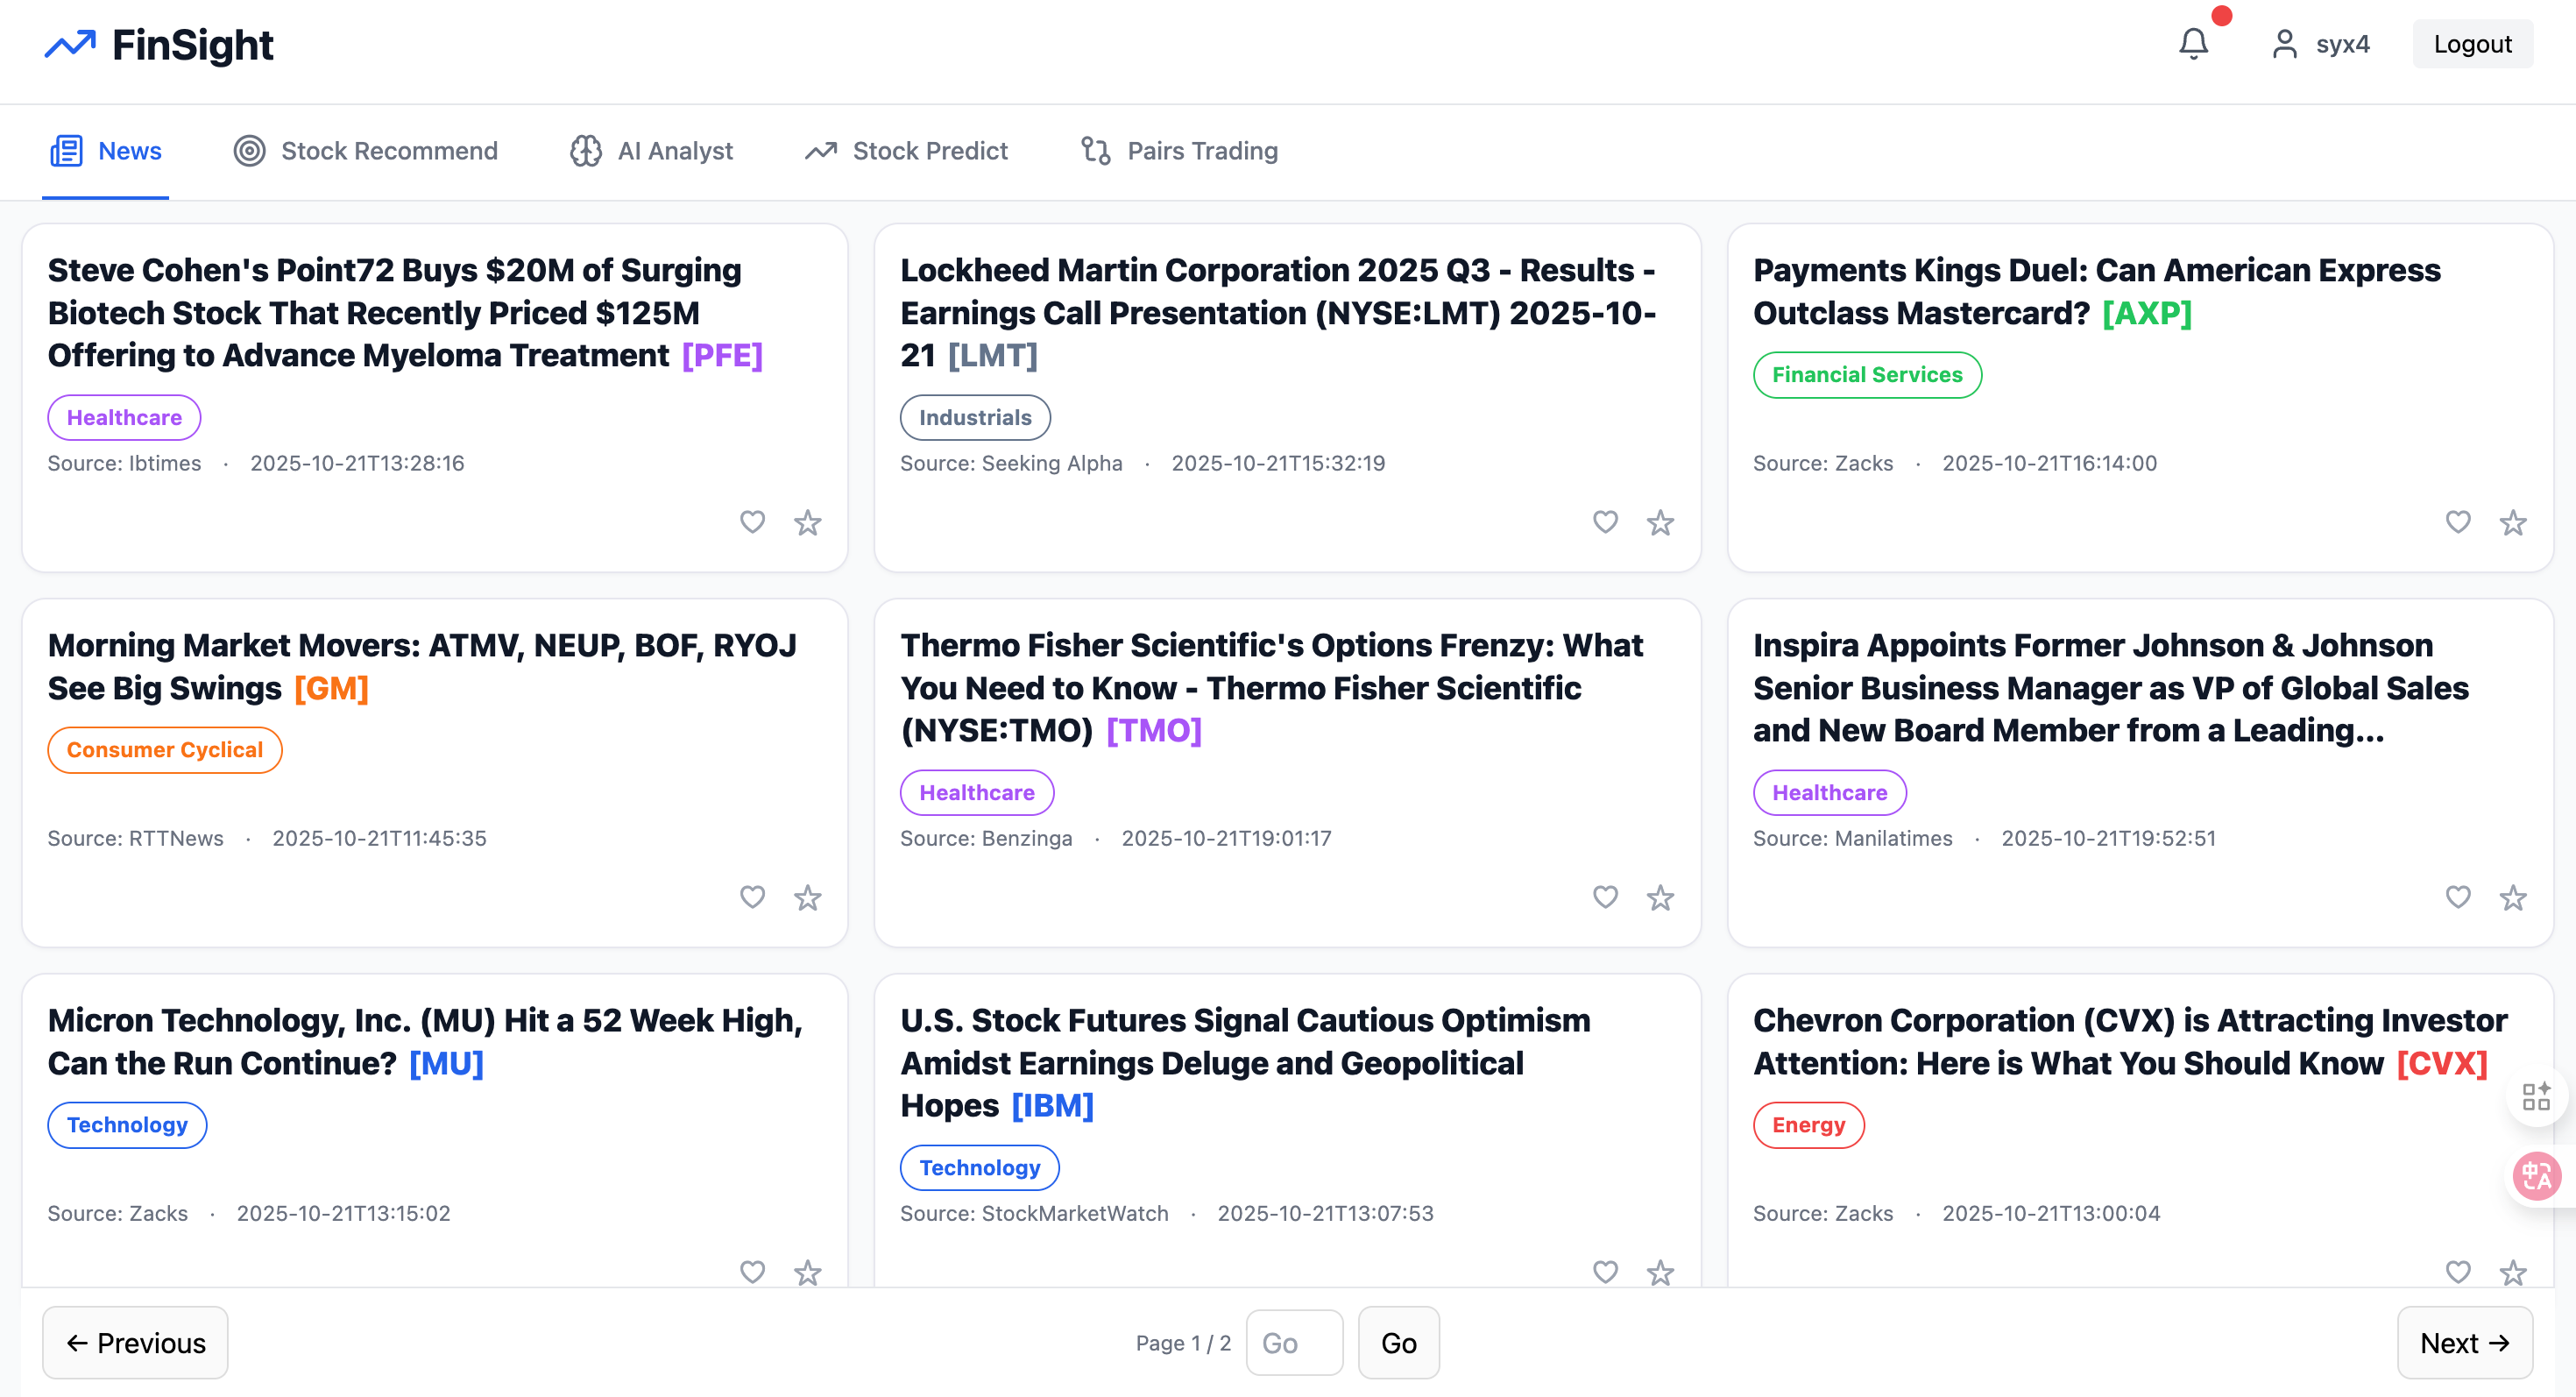
\includegraphics[width=0.9\textwidth]{images/news/page1.png}
% \caption{Initial News Feed Page Showing Personalized News Cards}
% \label{fig:news_page1}
% \end{figure}

% Figure \ref{fig:news_page1} illustrates the main news browsing interface, rendered in a \(3\times3\) card grid layout with smooth pagination. Each card presents the article’s title, ticker, sector tag, source, and publication date. The system retrieves these articles from the MongoDB-based news repository and applies the server-side ranking logic described earlier. Users can move between pages using \texttt{Previous}, \texttt{Next}, and direct page jump buttons, with cached navigation to minimize latency.

% When the user reaches the last page and triggers \texttt{Next}, the system enters the \textbf{trickle refresh mode}, dynamically fetching 1–3 new articles based on active tickers and seamlessly appending them to the local corpus. Figure \ref{fig:news_page2} shows the refreshed interface with new, unseen news items loaded.

% \begin{figure}[h]
% \centering
% 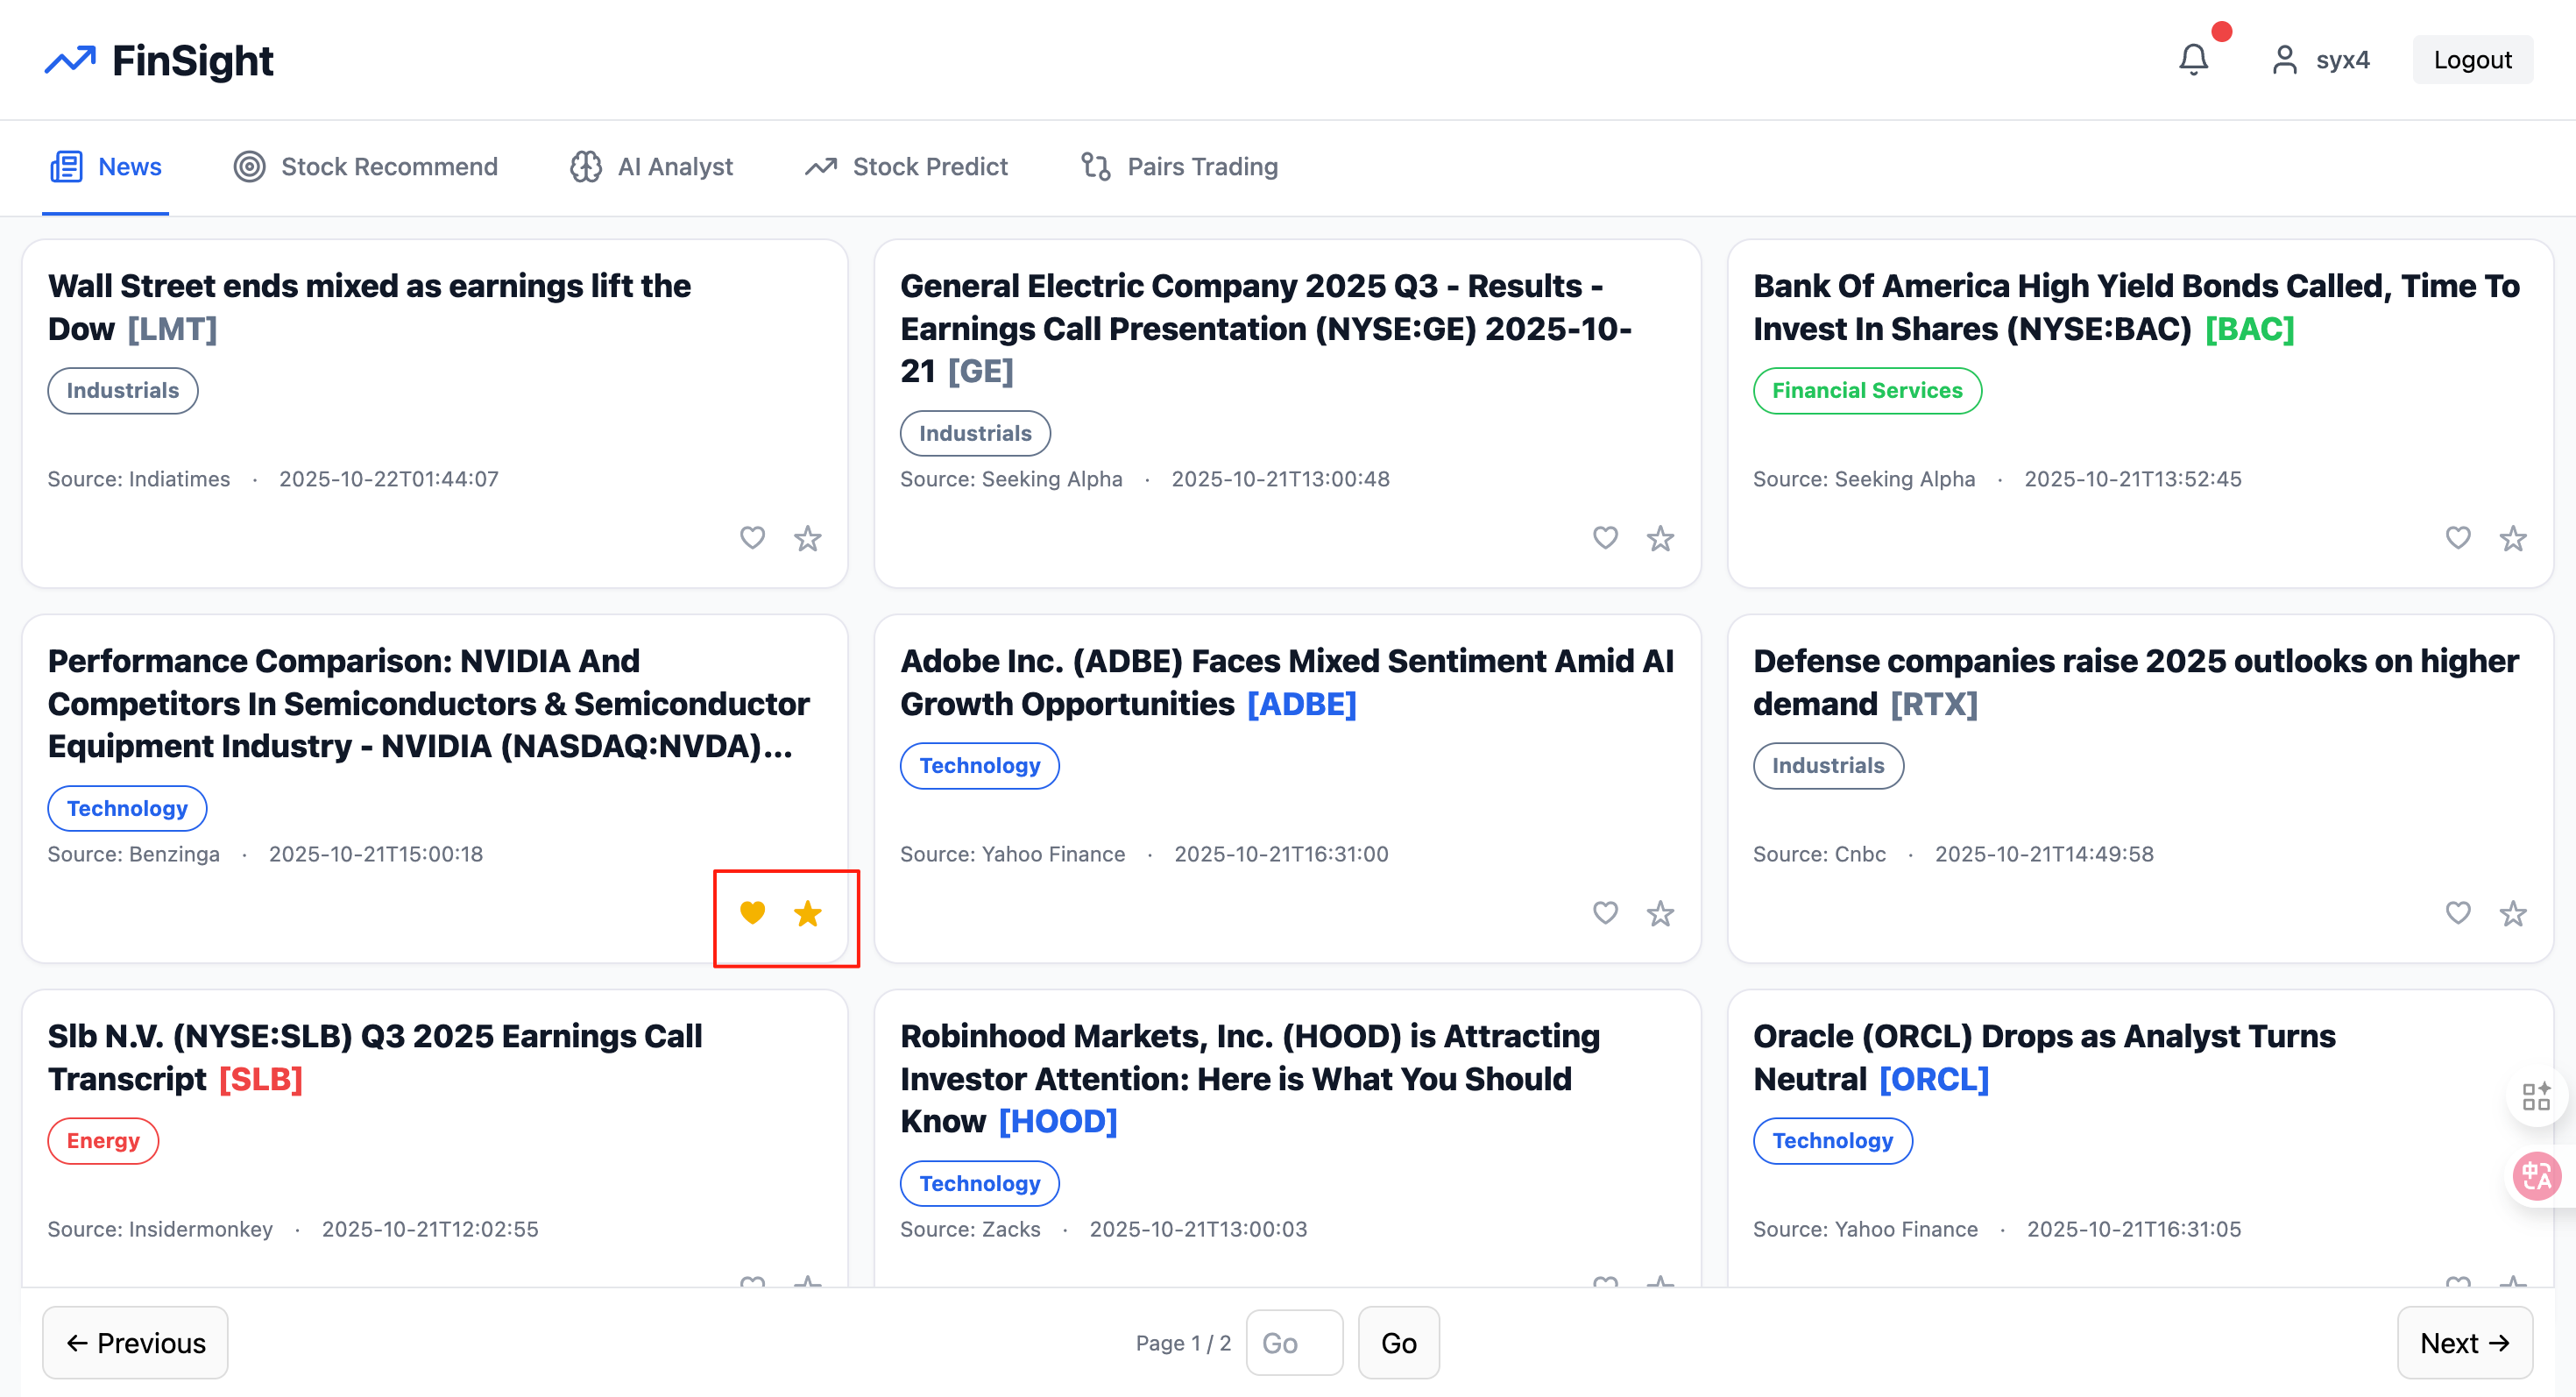
\includegraphics[width=0.9\textwidth]{images/news/page2.png}
% \caption{Trickle Refresh Mode Loading New Articles in Real-Time}
% \label{fig:news_page2}
% \end{figure}

% \textbf{2. User Interaction and Real-Time Vector Updates}

% The front-end enables three types of user interactions: \textbf{click}, \textbf{like}, and \textbf{bookmark}. These actions are recorded in MongoDB (\texttt{EventRepo}) and simultaneously update the user's 64-d semantic and 20-d preference vectors in PostgreSQL. 

% Figures \ref{fig:clk1} and \ref{fig:clk2} depict the process of a user liking a news article. The yellow heart/star icons represent a successful \texttt{like} action, which triggers the backend’s \texttt{update\_prof20\_add()} function in \texttt{PgProfileRepo}, adjusting the relevant preference dimensions.

% \begin{figure}[h]
% \centering
% 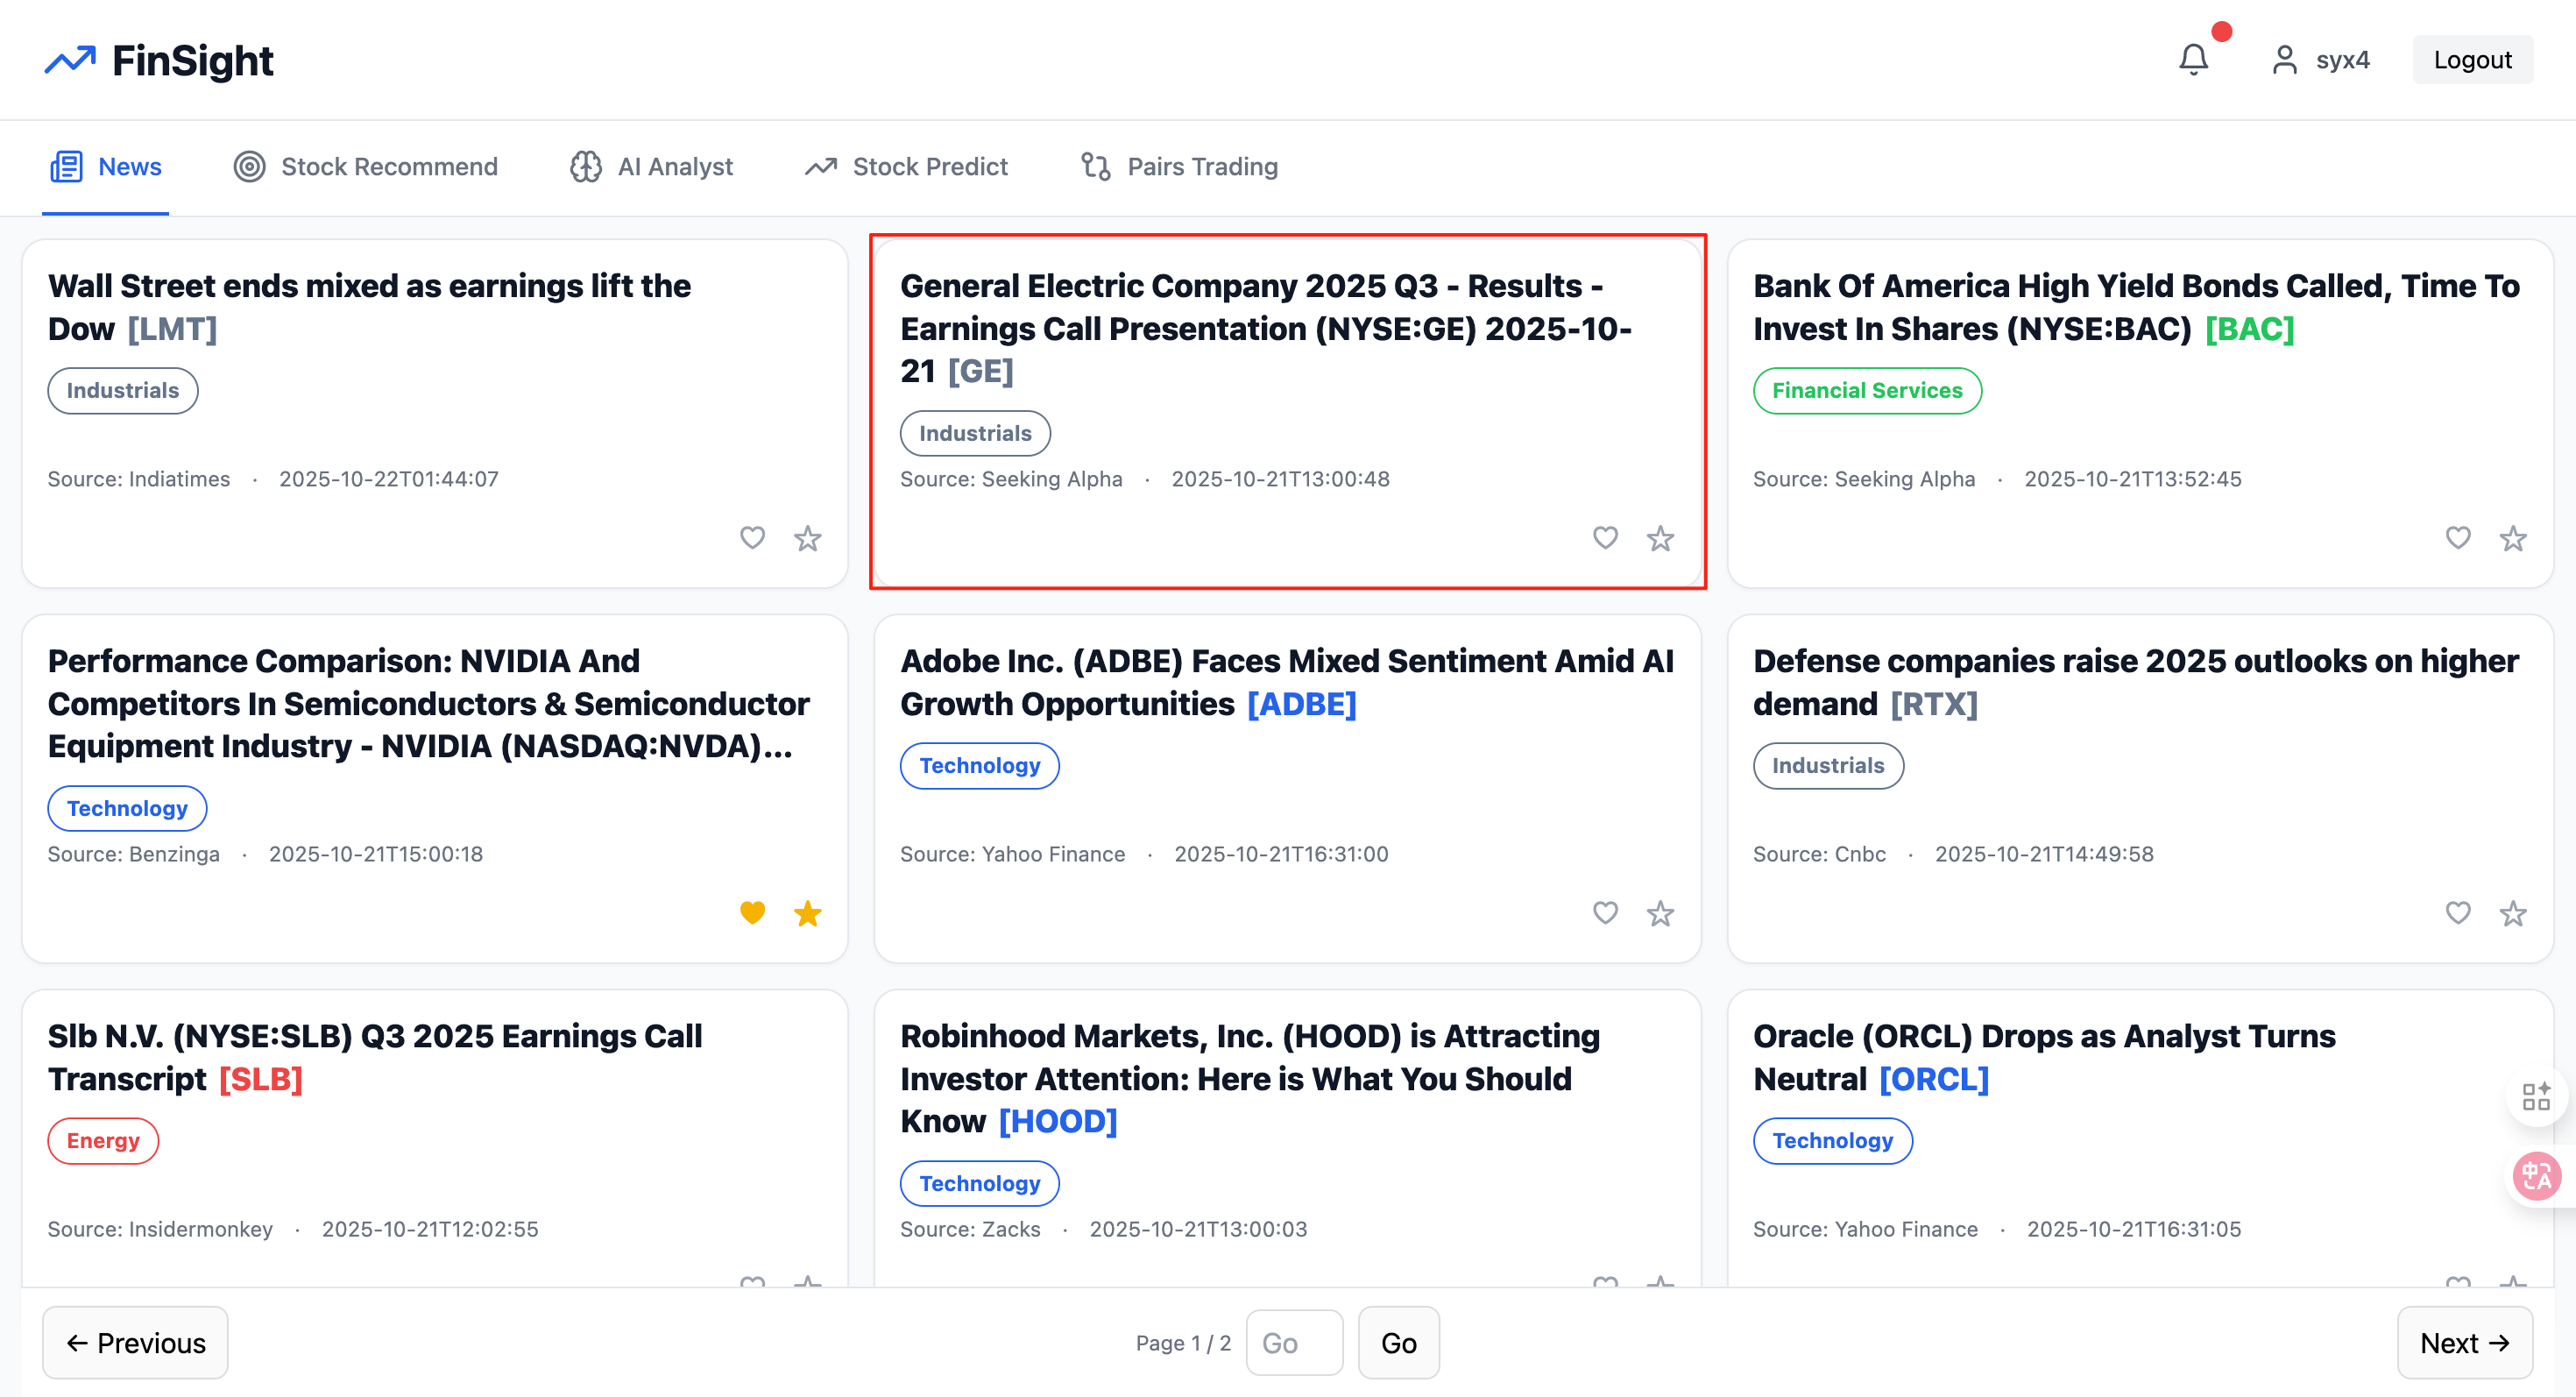
\includegraphics[width=0.8\textwidth]{images/news/clk1.png}
% \caption{User Performing Like and Bookmark Action on News Item}
% \label{fig:clk1}
% \end{figure}

% \begin{figure}[h]
% \centering
% 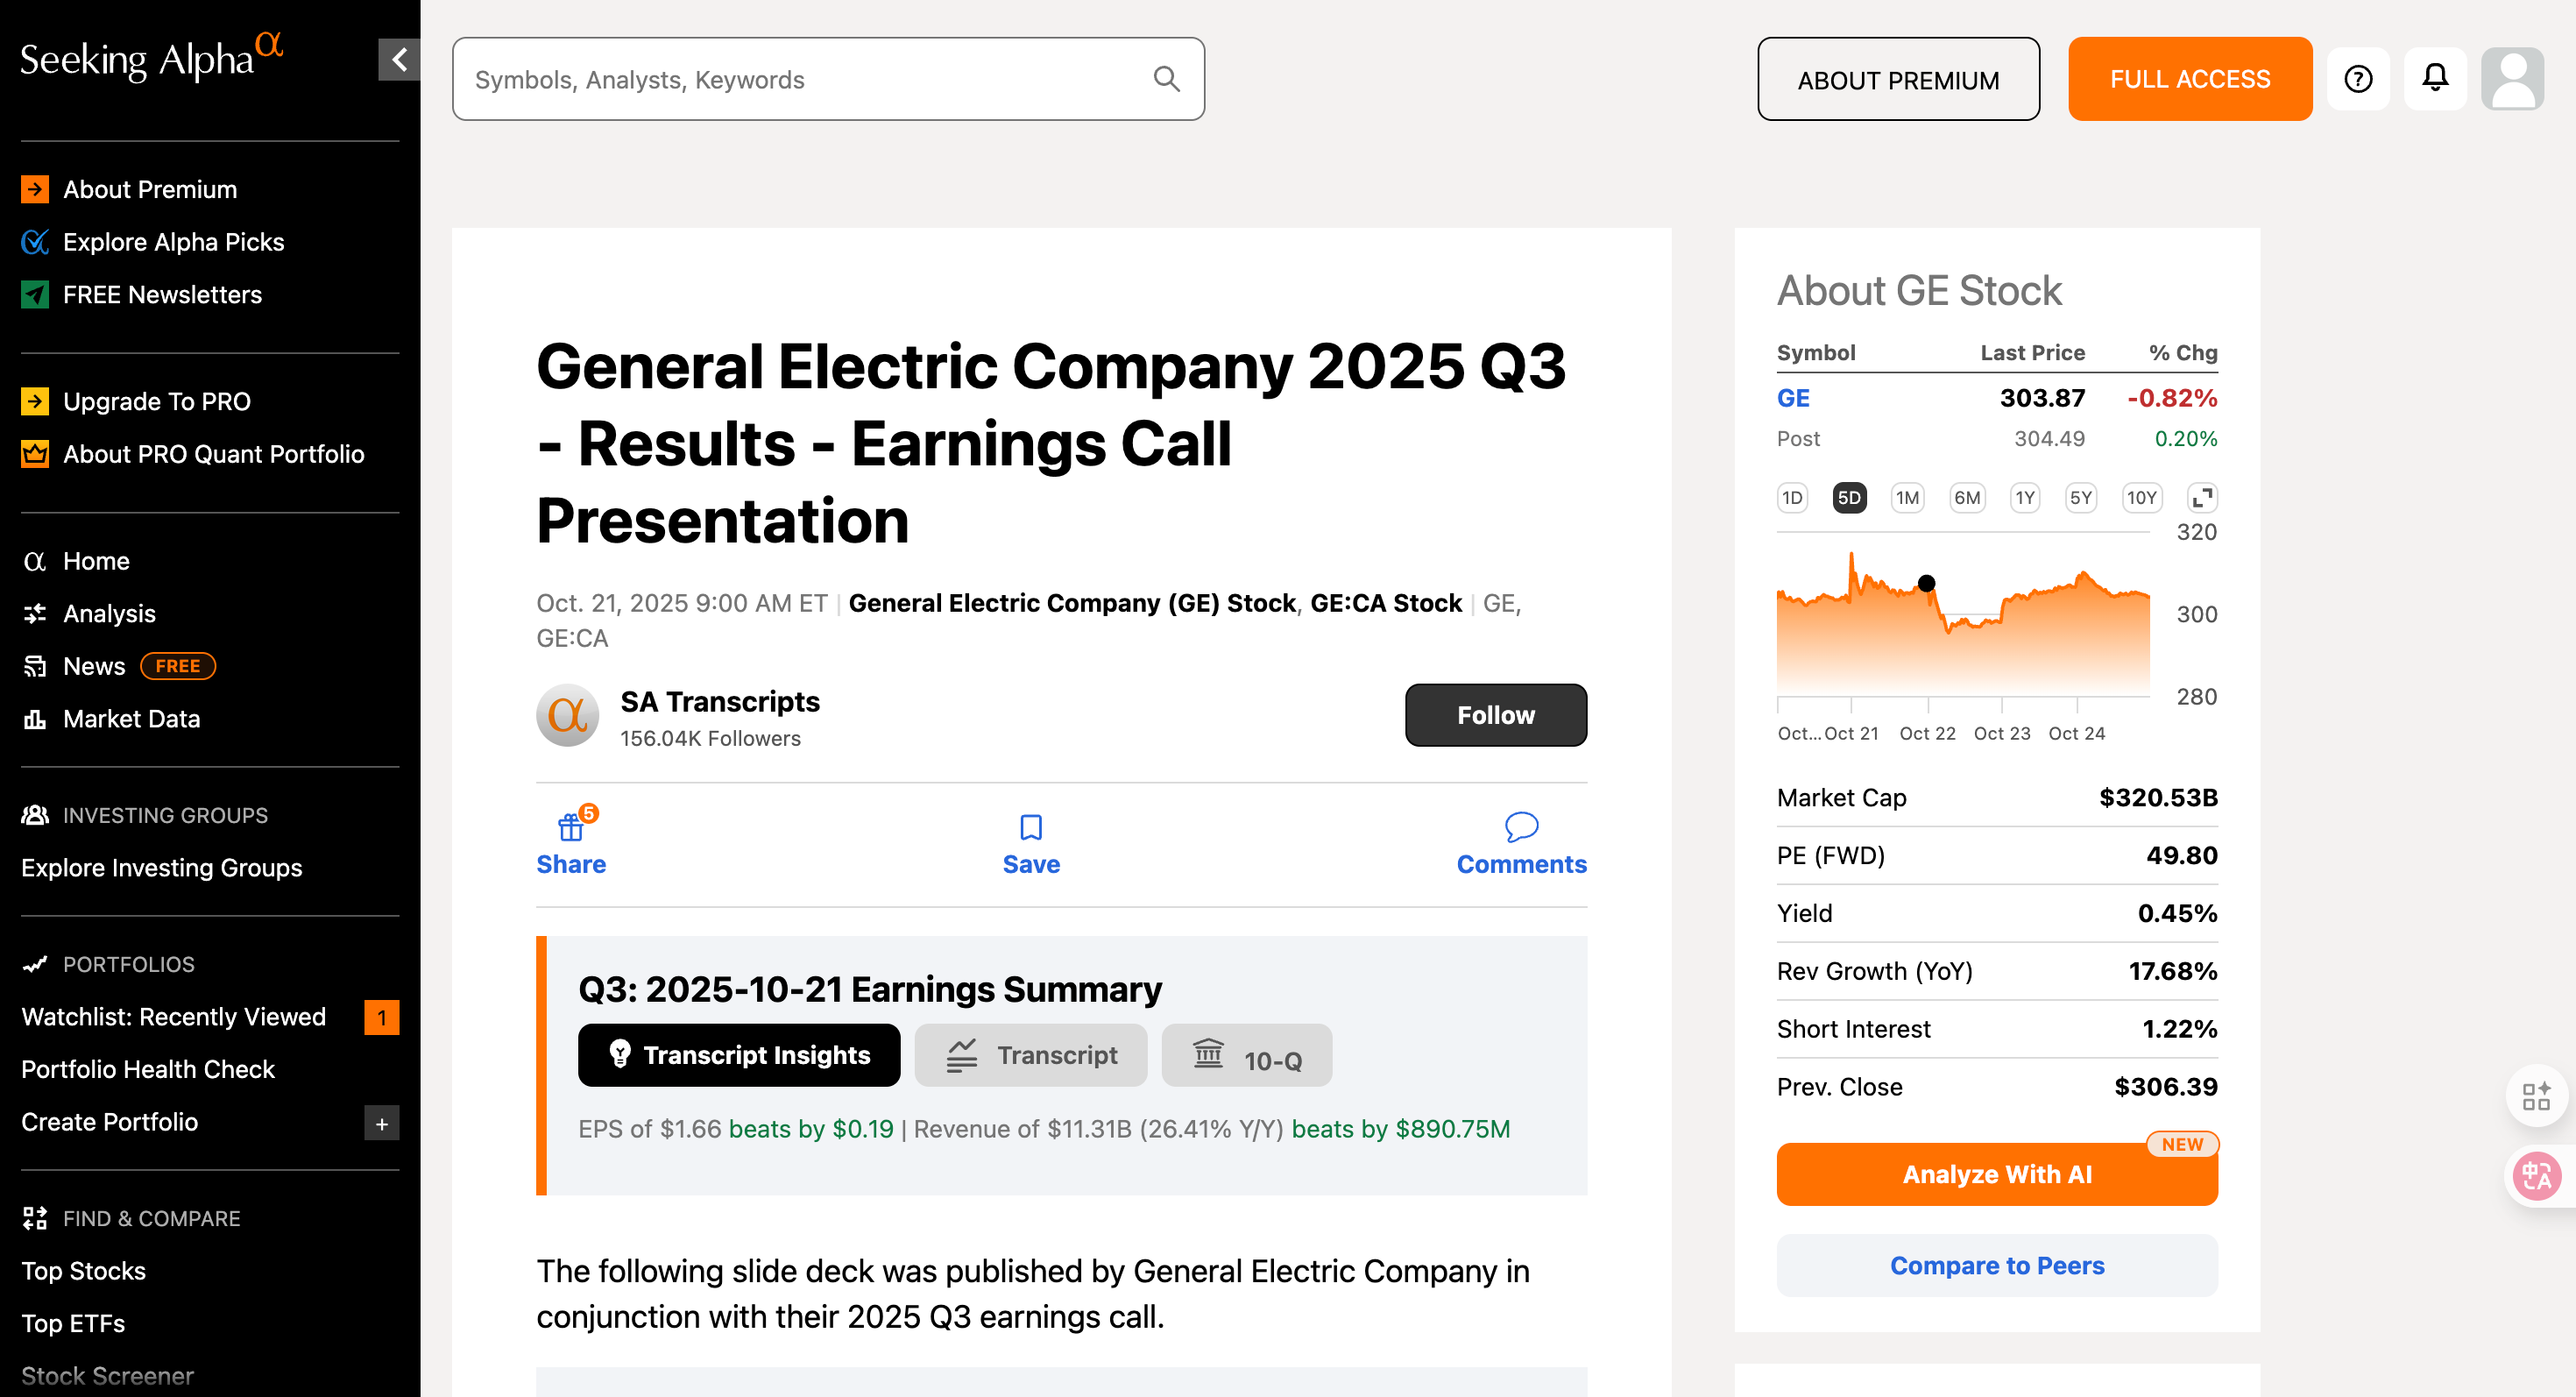
\includegraphics[width=0.8\textwidth]{images/news/clk2.png}
% \caption{Updated Preference Reflected in UI and Database}
% \label{fig:clk2}
% \end{figure}

% \textbf{3. Back-End Profile Evolution Verification}

% To verify personalization, we track vector changes before and after user actions. Figures \ref{fig:20d1} and \ref{fig:20d2} show the evolution of the 20-dimensional preference vector (\texttt{profile\_vector\_20d}), where the highlighted component (e.g., industrial sector dimension) increased after the user liked a relevant article.

% \begin{figure}[h]
% \centering
% 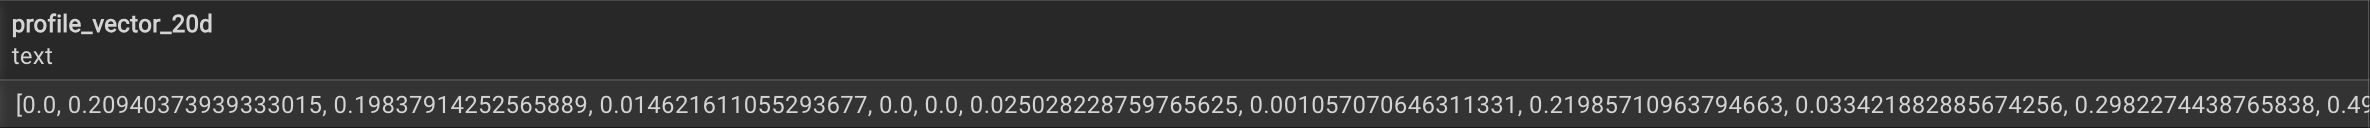
\includegraphics[width=0.8\textwidth]{images/news/20d1.png}
% \caption{User 20-D Preference Vector Before Interaction}
% \label{fig:20d1}
% \end{figure}

% \begin{figure}[h]
% \centering
% 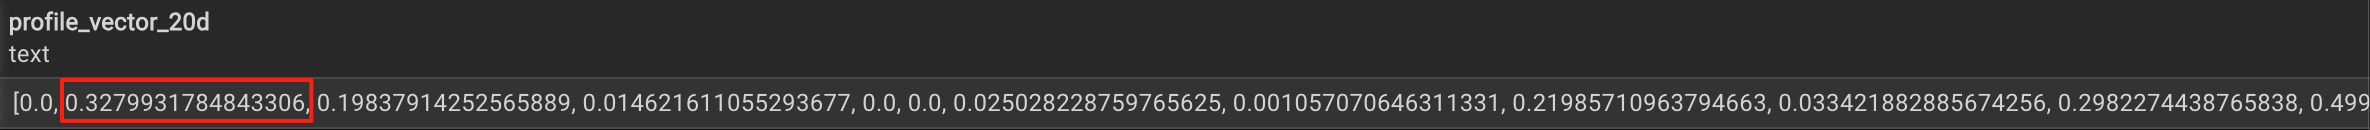
\includegraphics[width=0.8\textwidth]{images/news/20d2.png}
% \caption{User 20-D Preference Vector After Interaction: Technology Weight Increased}
% \label{fig:20d2}
% \end{figure}

% Similarly, Figures \ref{fig:64d1} and \ref{fig:64d2} present the 64-dimensional short-term semantic embedding (\texttt{user\_semantic\_64d\_short}), which undergoes slight EMA-based shifts reflecting the article’s content vector. These changes collectively guide ranking adjustments for subsequent recommendations.

% \textbf{4. Live Personalization and Feedback Loop}

% As the vectors evolve, the ranking service recalculates cosine similarities between the updated user vector \(\mathbf{u}\) and article vectors \(\mathbf{p}_a\), reordering results on subsequent refreshes. This ensures that after a user interacts with specific sectors (e.g., Technology or Industrials), the following pages emphasize those preferences while maintaining diversity.

% \begin{figure}[h]
% \centering
% 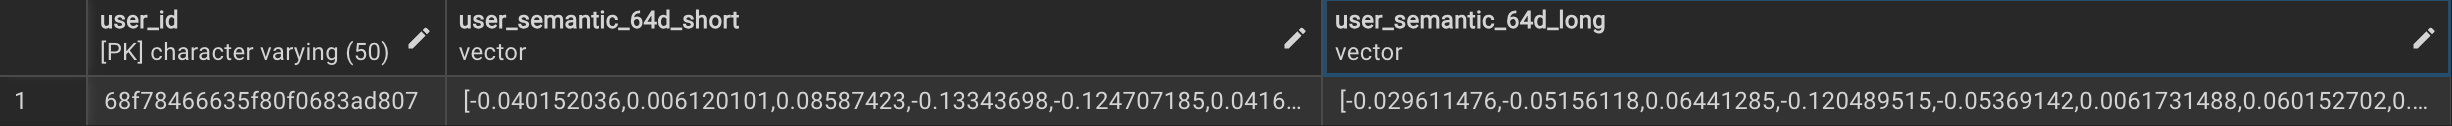
\includegraphics[width=0.8\textwidth]{images/news/64d1.png}
% \caption{User 64-D Semantic Vector Before Interaction}
% \label{fig:64d1}
% \end{figure}

% \begin{figure}[h]
% \centering
% 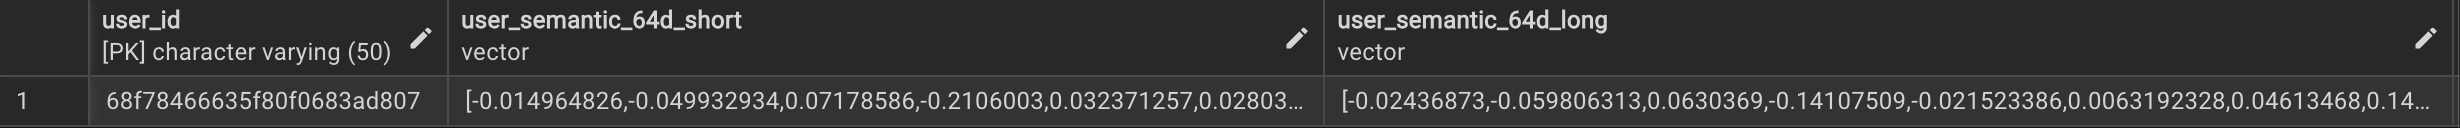
\includegraphics[width=0.8\textwidth]{images/news/64d2.png}
% \caption{User 64-D Semantic Vector After Interaction: Content-Driven Update Applied(click)}
% \label{fig:64d2}
% \end{figure}



% \subsection{Technical Validation and Performance}

% \begin{table}[h]
% \centering
% \caption{System Component Integration Validation for News Module}
% \begin{tabular}{|p{5cm}|p{8cm}|}
% \hline
% \textbf{Component} & \textbf{Validation Result} \\
% \hline
% Frontend-Backend Integration & React front-end communicates with FastAPI backend seamlessly; event logging and vector updates confirmed in real time. \\
% \hline
% Data Pipeline Integration & Google RSS and Marketaux APIs successfully fetch fresh news data; MongoDB upsert and de-duplication verified. \\
% \hline
% Database Schema Consistency & PostgreSQL 64d/20d vectors and JSON mirrors remain synchronized; type safety verified after feedback actions. \\
% \hline
% Exclude-Seen and Ranking & Sliding-window filtering correctly removes recently read articles; ranking reflects both recency and preference match. \\
% \hline
% System Latency & Typical \texttt{/rec/user/news} response time: 120–180 ms (cached mode); under 250 ms with refresh-enabled fetch. \\
% \hline
% \end{tabular}
% \end{table}

% \textbf{User Experience and Responsiveness}

% The interface achieves high responsiveness and transparency:
% \begin{itemize}
% \item Instant page transitions with cached data and async re-ranking
% \item Dynamic icon toggling for likes/bookmarks without reloads
% \item Smooth integration of new articles under \texttt{refresh=1}
% \item Real-time user preference shaping reflected in subsequent recommendations
% \end{itemize}



\section{News Browsing Module}

\subsection{System Functionality Demonstration}

The News Browsing Module has been fully implemented and integrated into the FinSight platform. This section demonstrates the key functionalities of the module—news fetching, ranking, user interaction, and personalization—alongside actual screenshots from the deployed system.

\textbf{1. Core Interface and Pagination System}

\begin{figure}[H]
  \centering
  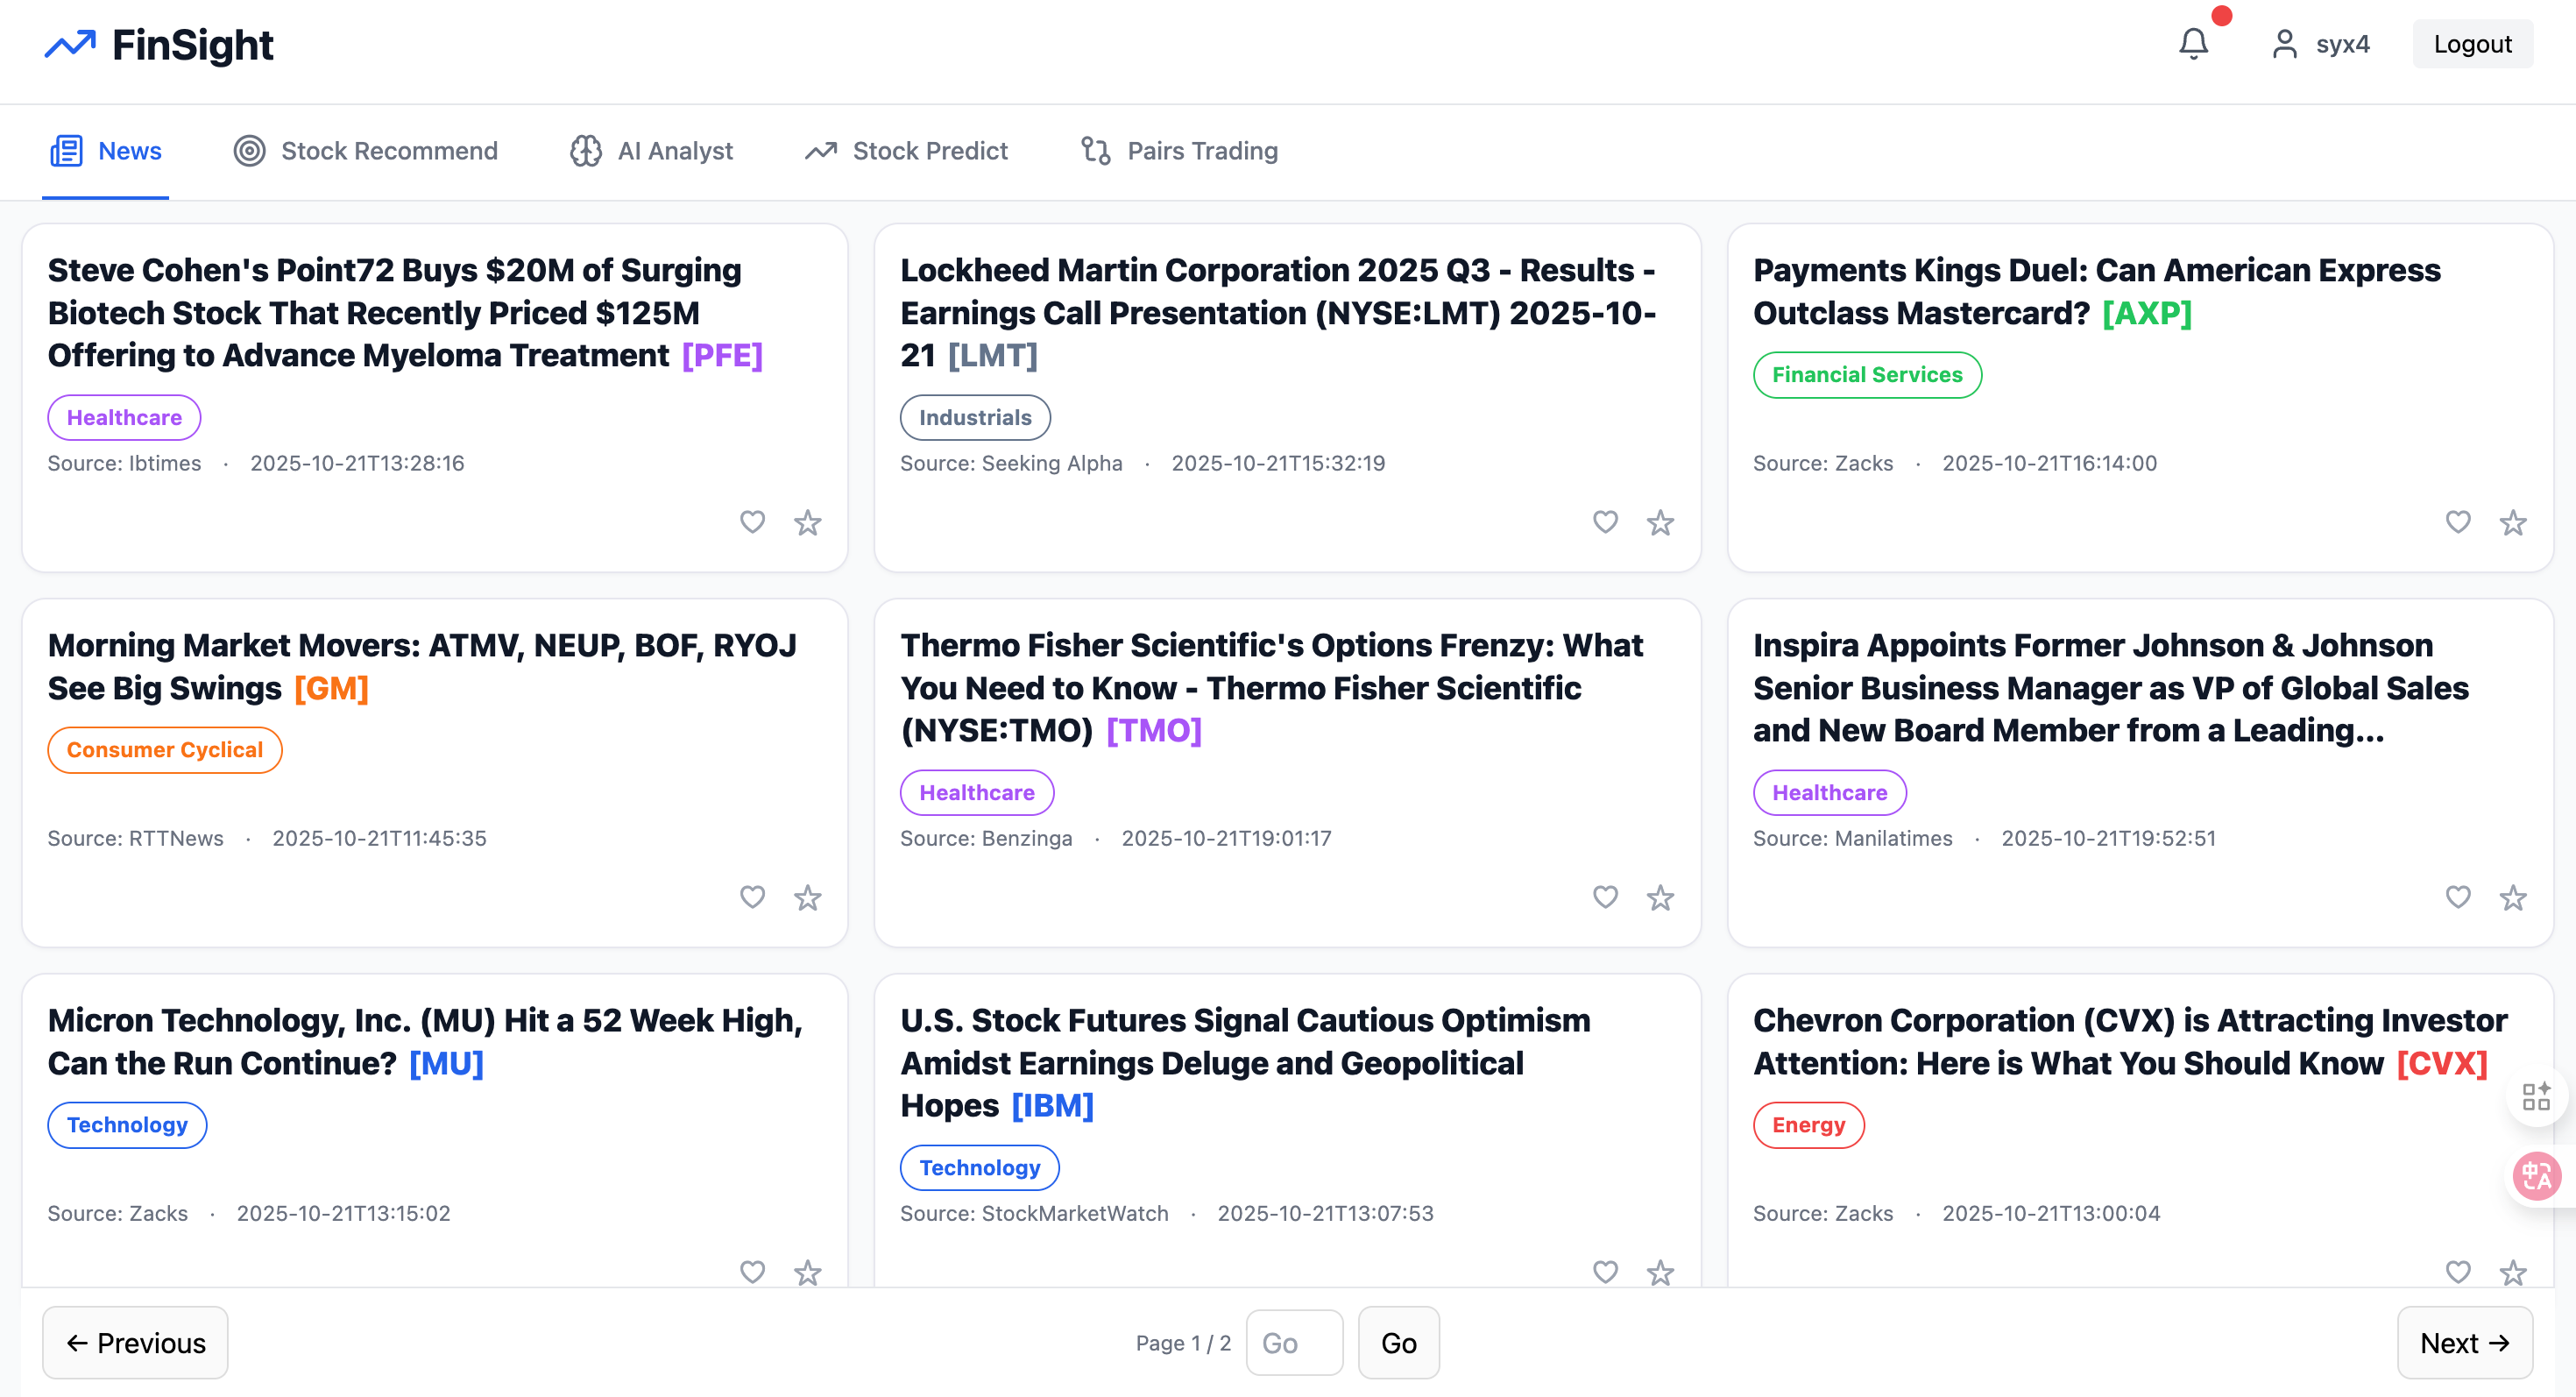
\includegraphics[width=0.92\textwidth]{images/news/page1.png}
  \caption{Initial News Feed Page Showing Personalized News Cards}
  \label{fig:news_page1}
\end{figure}

Figure~\ref{fig:news_page1} illustrates the main news browsing interface, rendered in a \(3\times3\) card grid layout with smooth pagination. Each card presents the article’s title, ticker, sector tag, source, and publication date. The system retrieves these articles from the MongoDB-based news repository and applies the server-side ranking logic described earlier. Users can move between pages using \texttt{Previous}, \texttt{Next}, and direct page jump buttons, with cached navigation to minimize latency.

When the user reaches the last page and triggers \texttt{Next}, the system enters the \textbf{trickle refresh mode}, dynamically fetching 1–3 new articles based on active tickers and seamlessly appending them to the local corpus.

\begin{figure}[H]
  \centering
  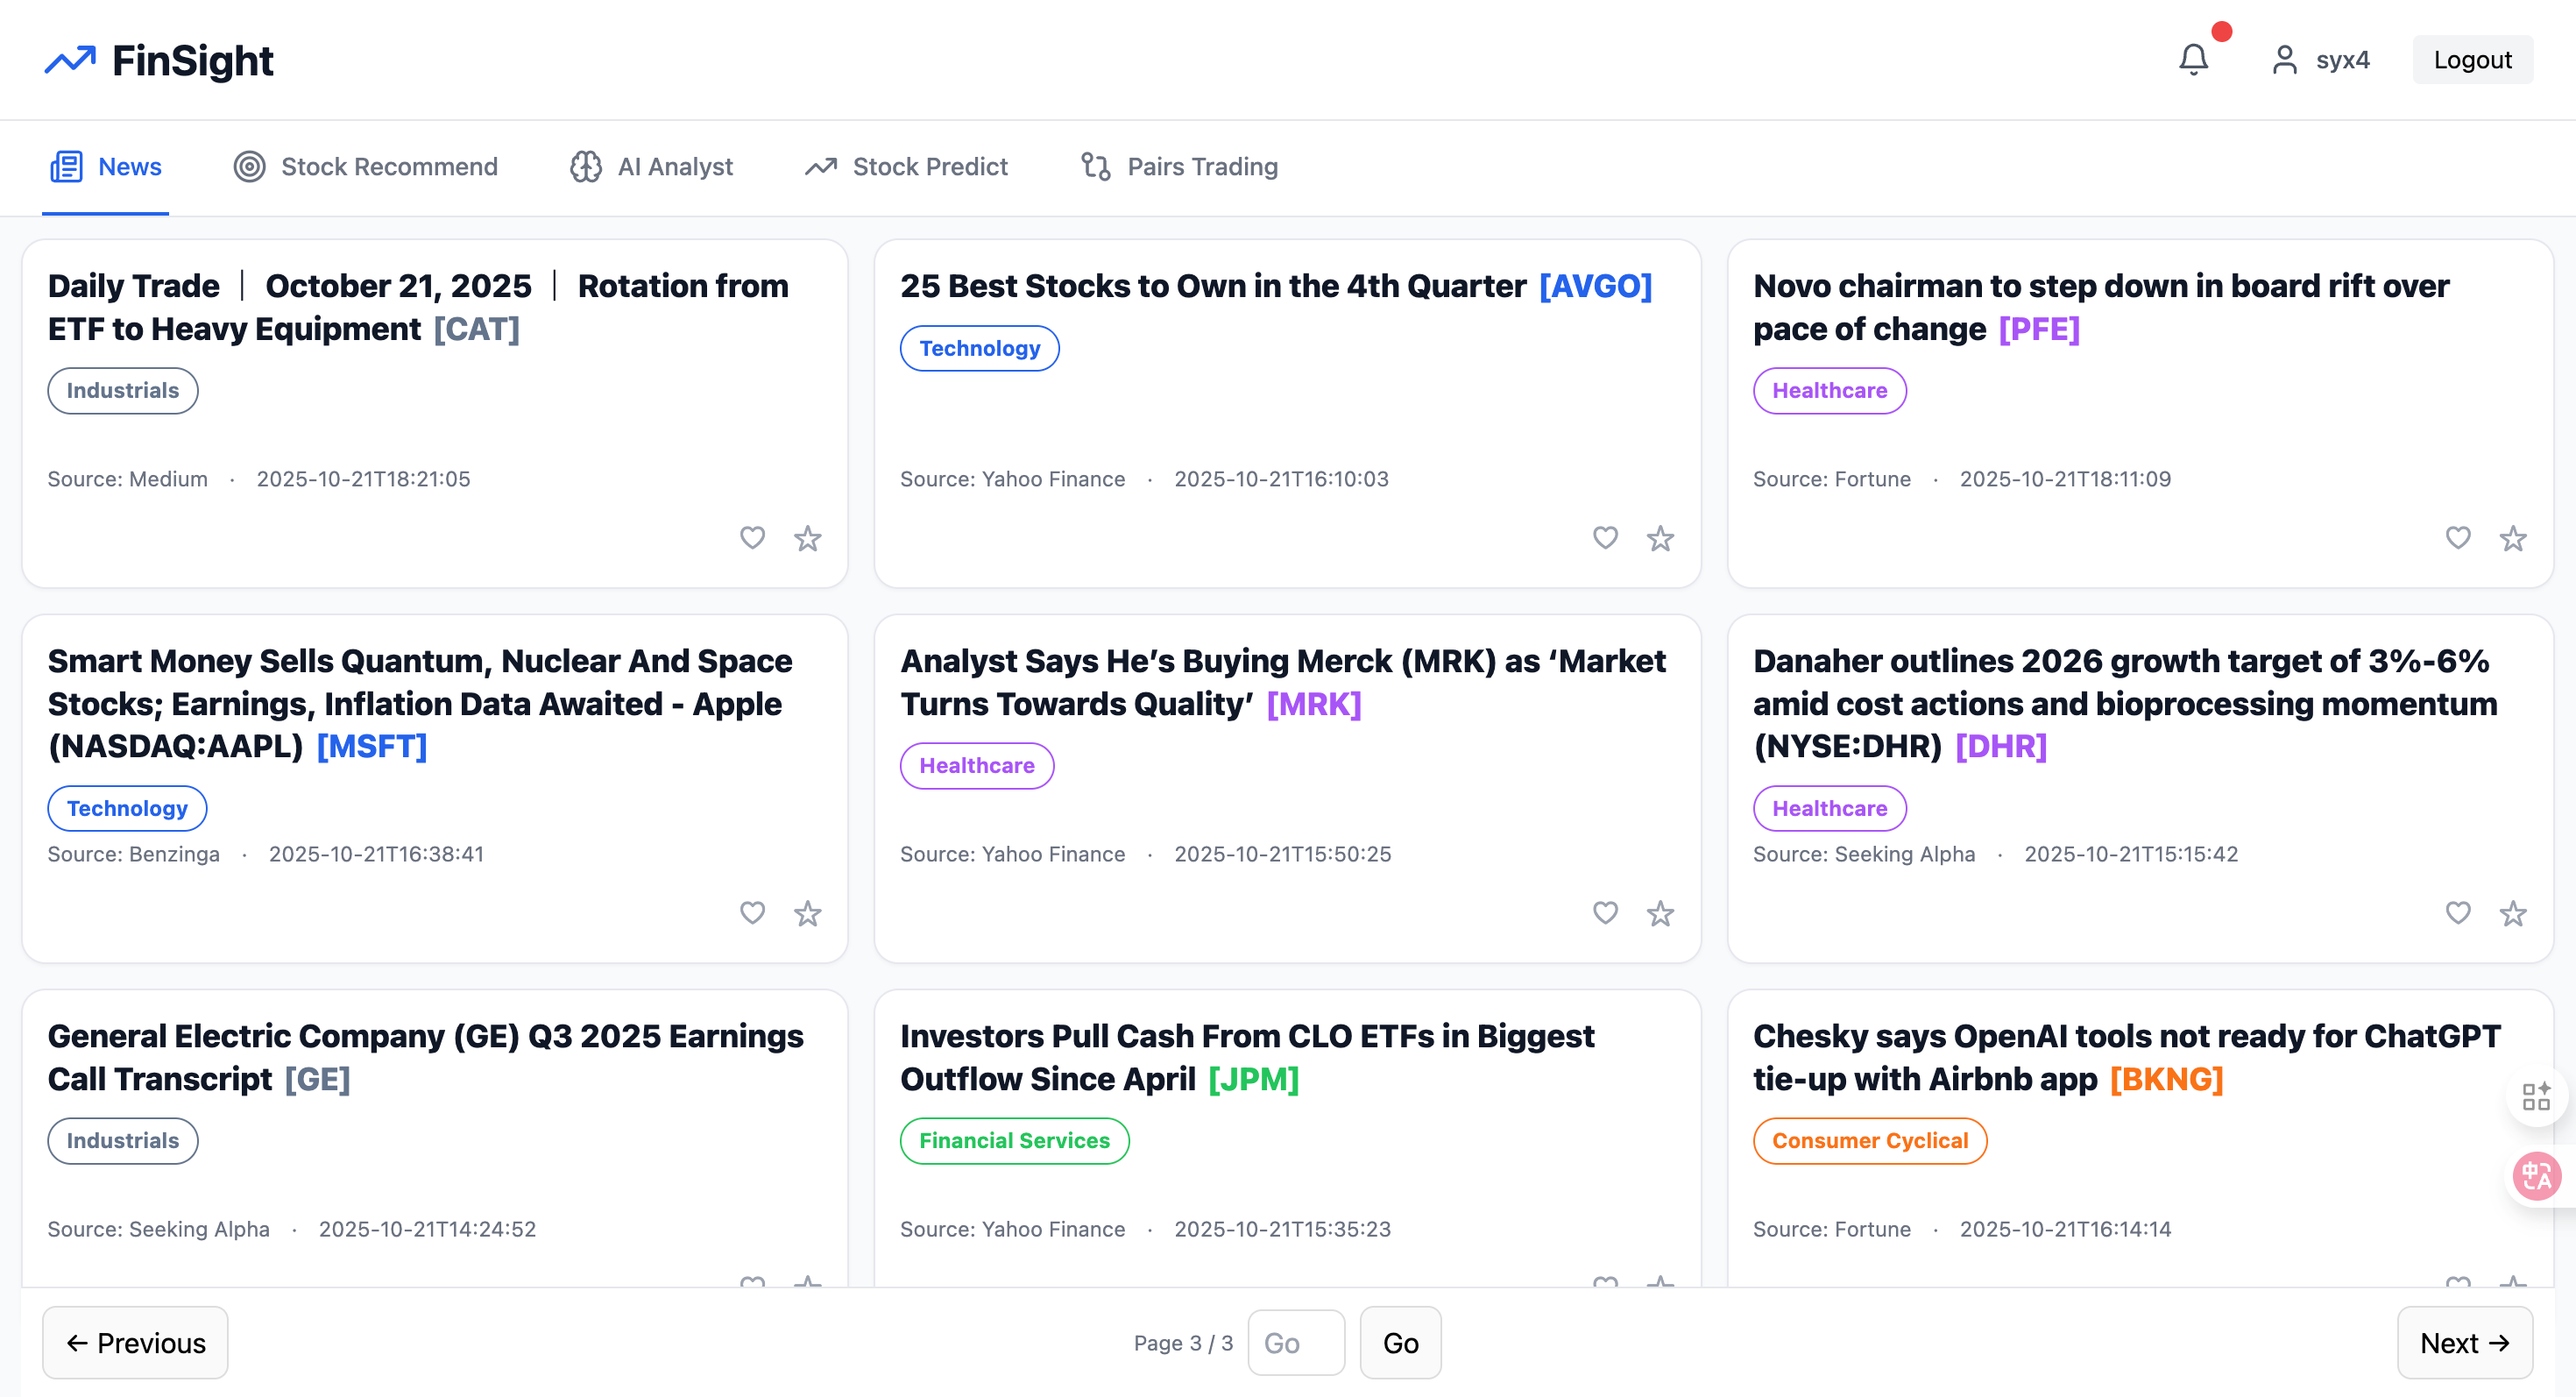
\includegraphics[width=0.92\textwidth]{images/news/refresh.png}
  \caption{Trickle Refresh Mode Loading New Articles in Real-Time}
  \label{fig:refresh}
\end{figure}

\textbf{2. User Interaction and Real-Time Vector Updates}

The front-end enables three types of user interactions: \textbf{click}, \textbf{like}, and \textbf{bookmark}. These actions are recorded in MongoDB (\texttt{EventRepo}) and simultaneously update the user's 64-d semantic and 20-d preference vectors in PostgreSQL.

\begin{figure}[H]
  \centering
  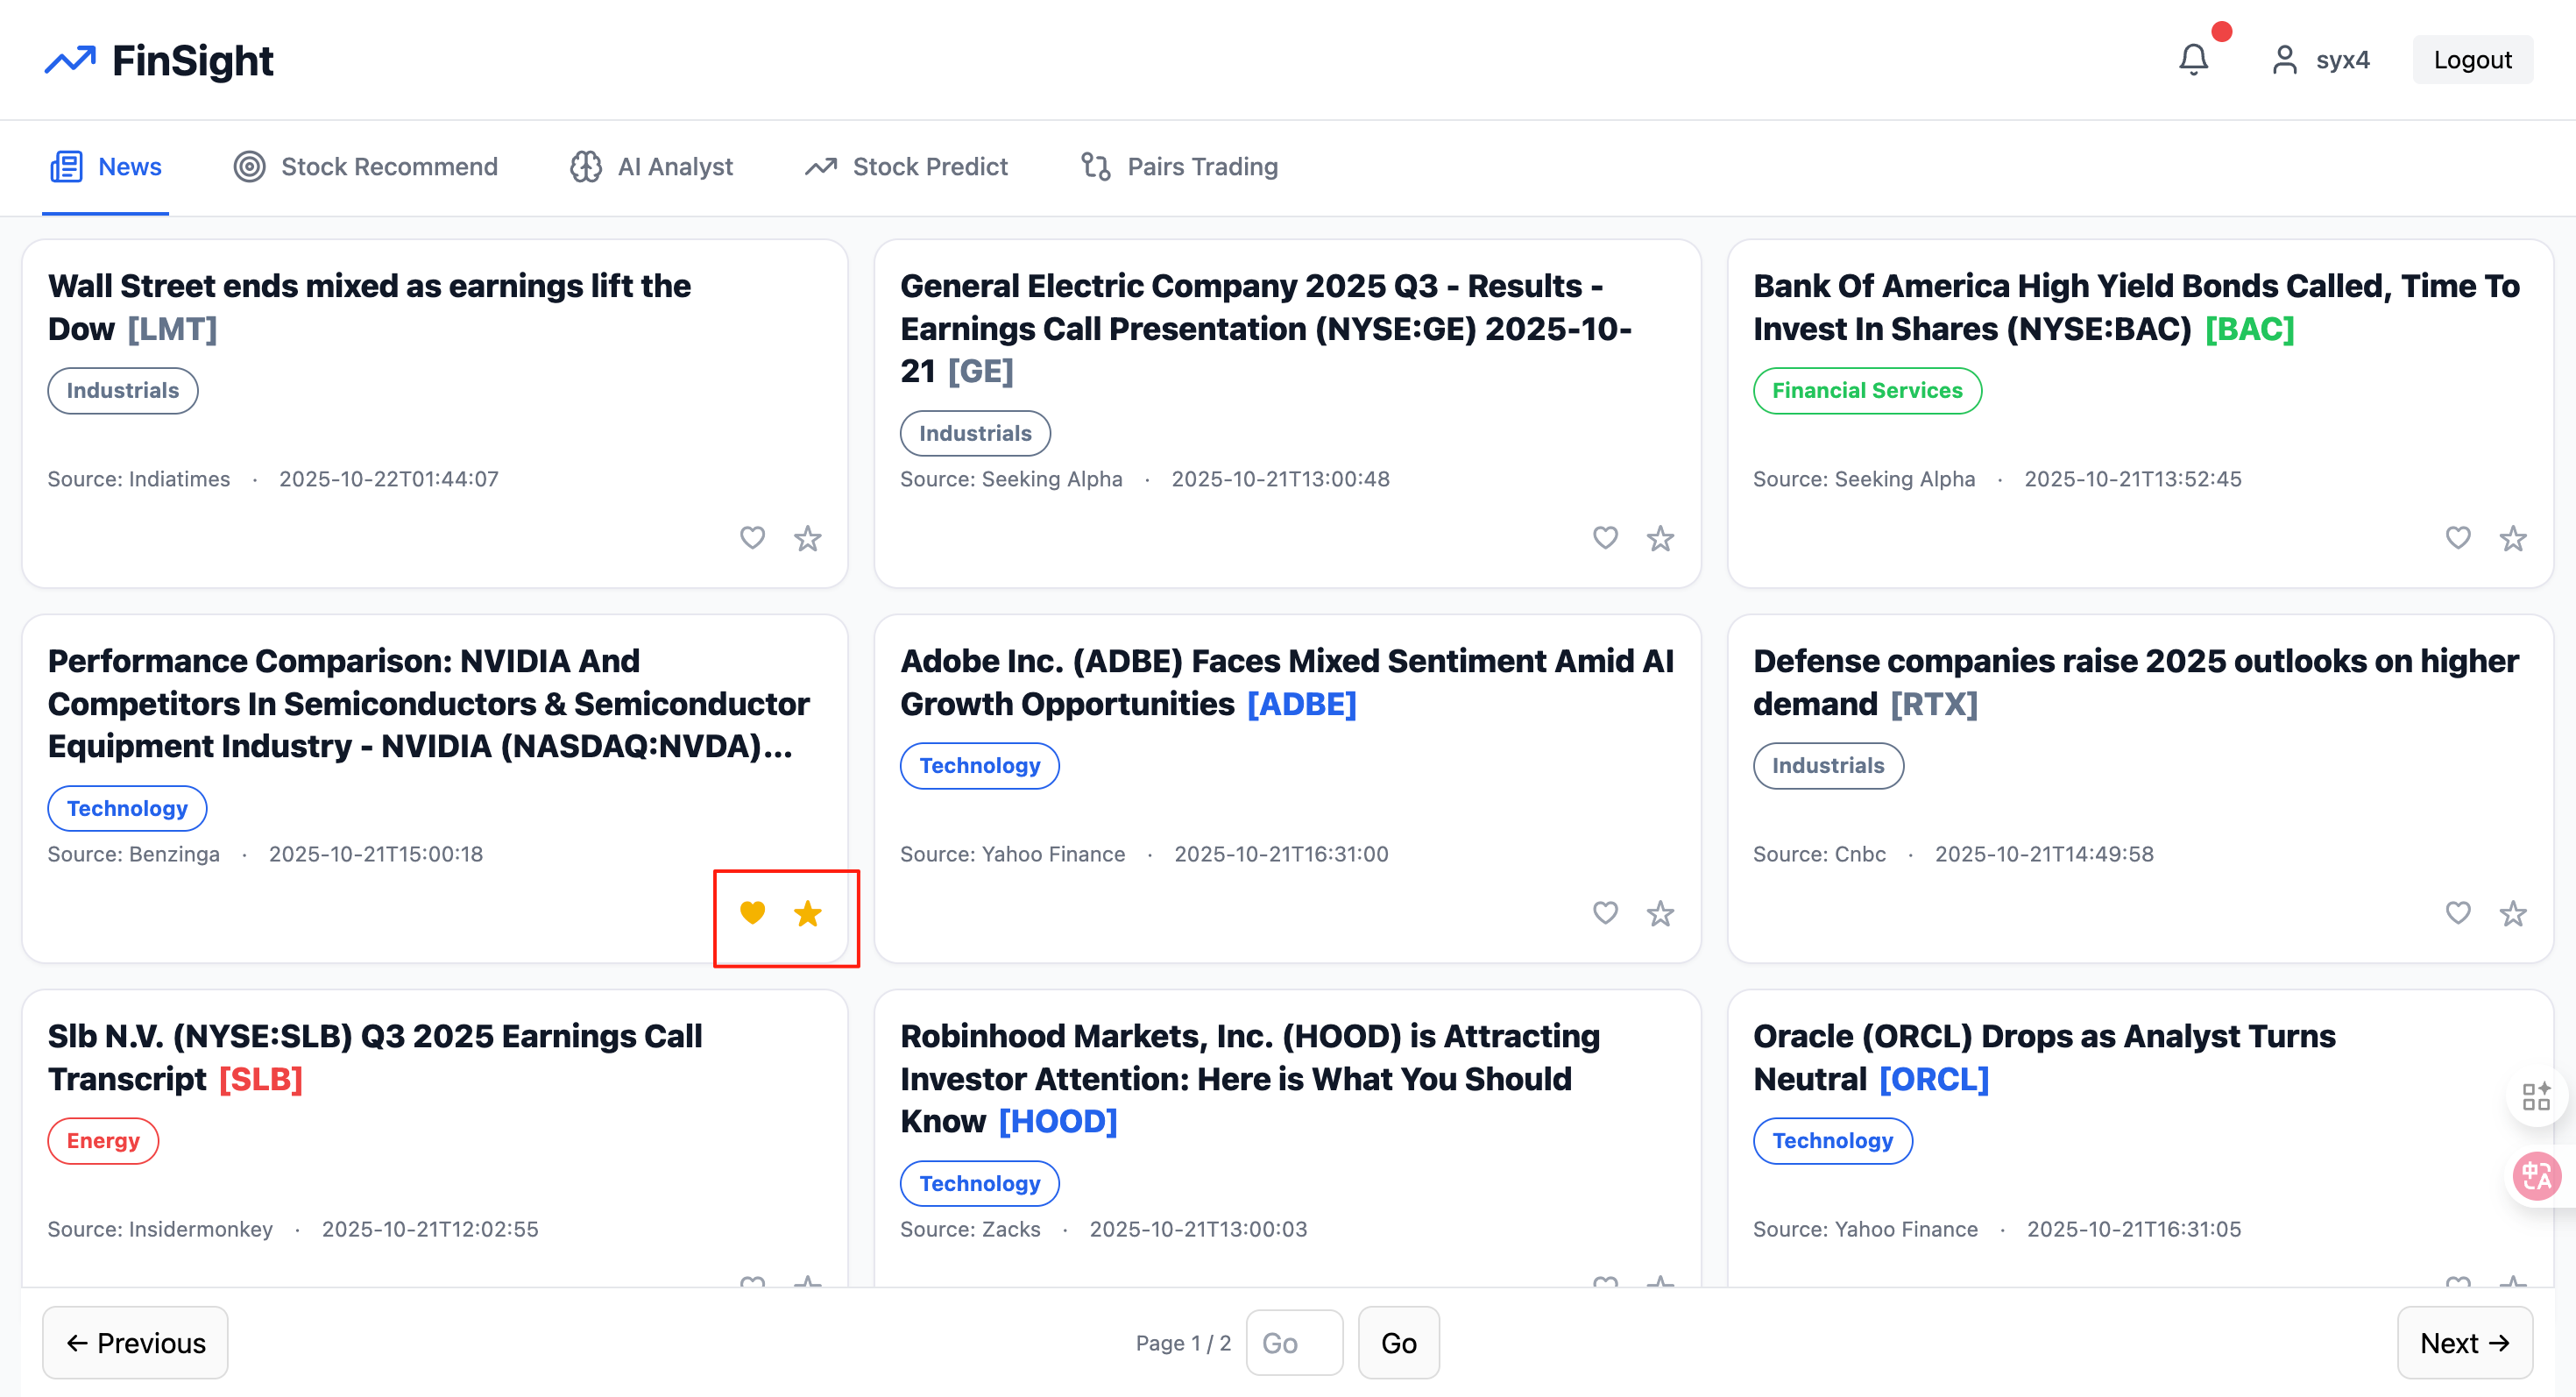
\includegraphics[width=0.82\textwidth]{images/news/page2.png}
  \caption{User Performing Like and Bookmark Action on News Item}
  \label{fig:page2}
\end{figure}


\begin{figure}[H]
  \centering
  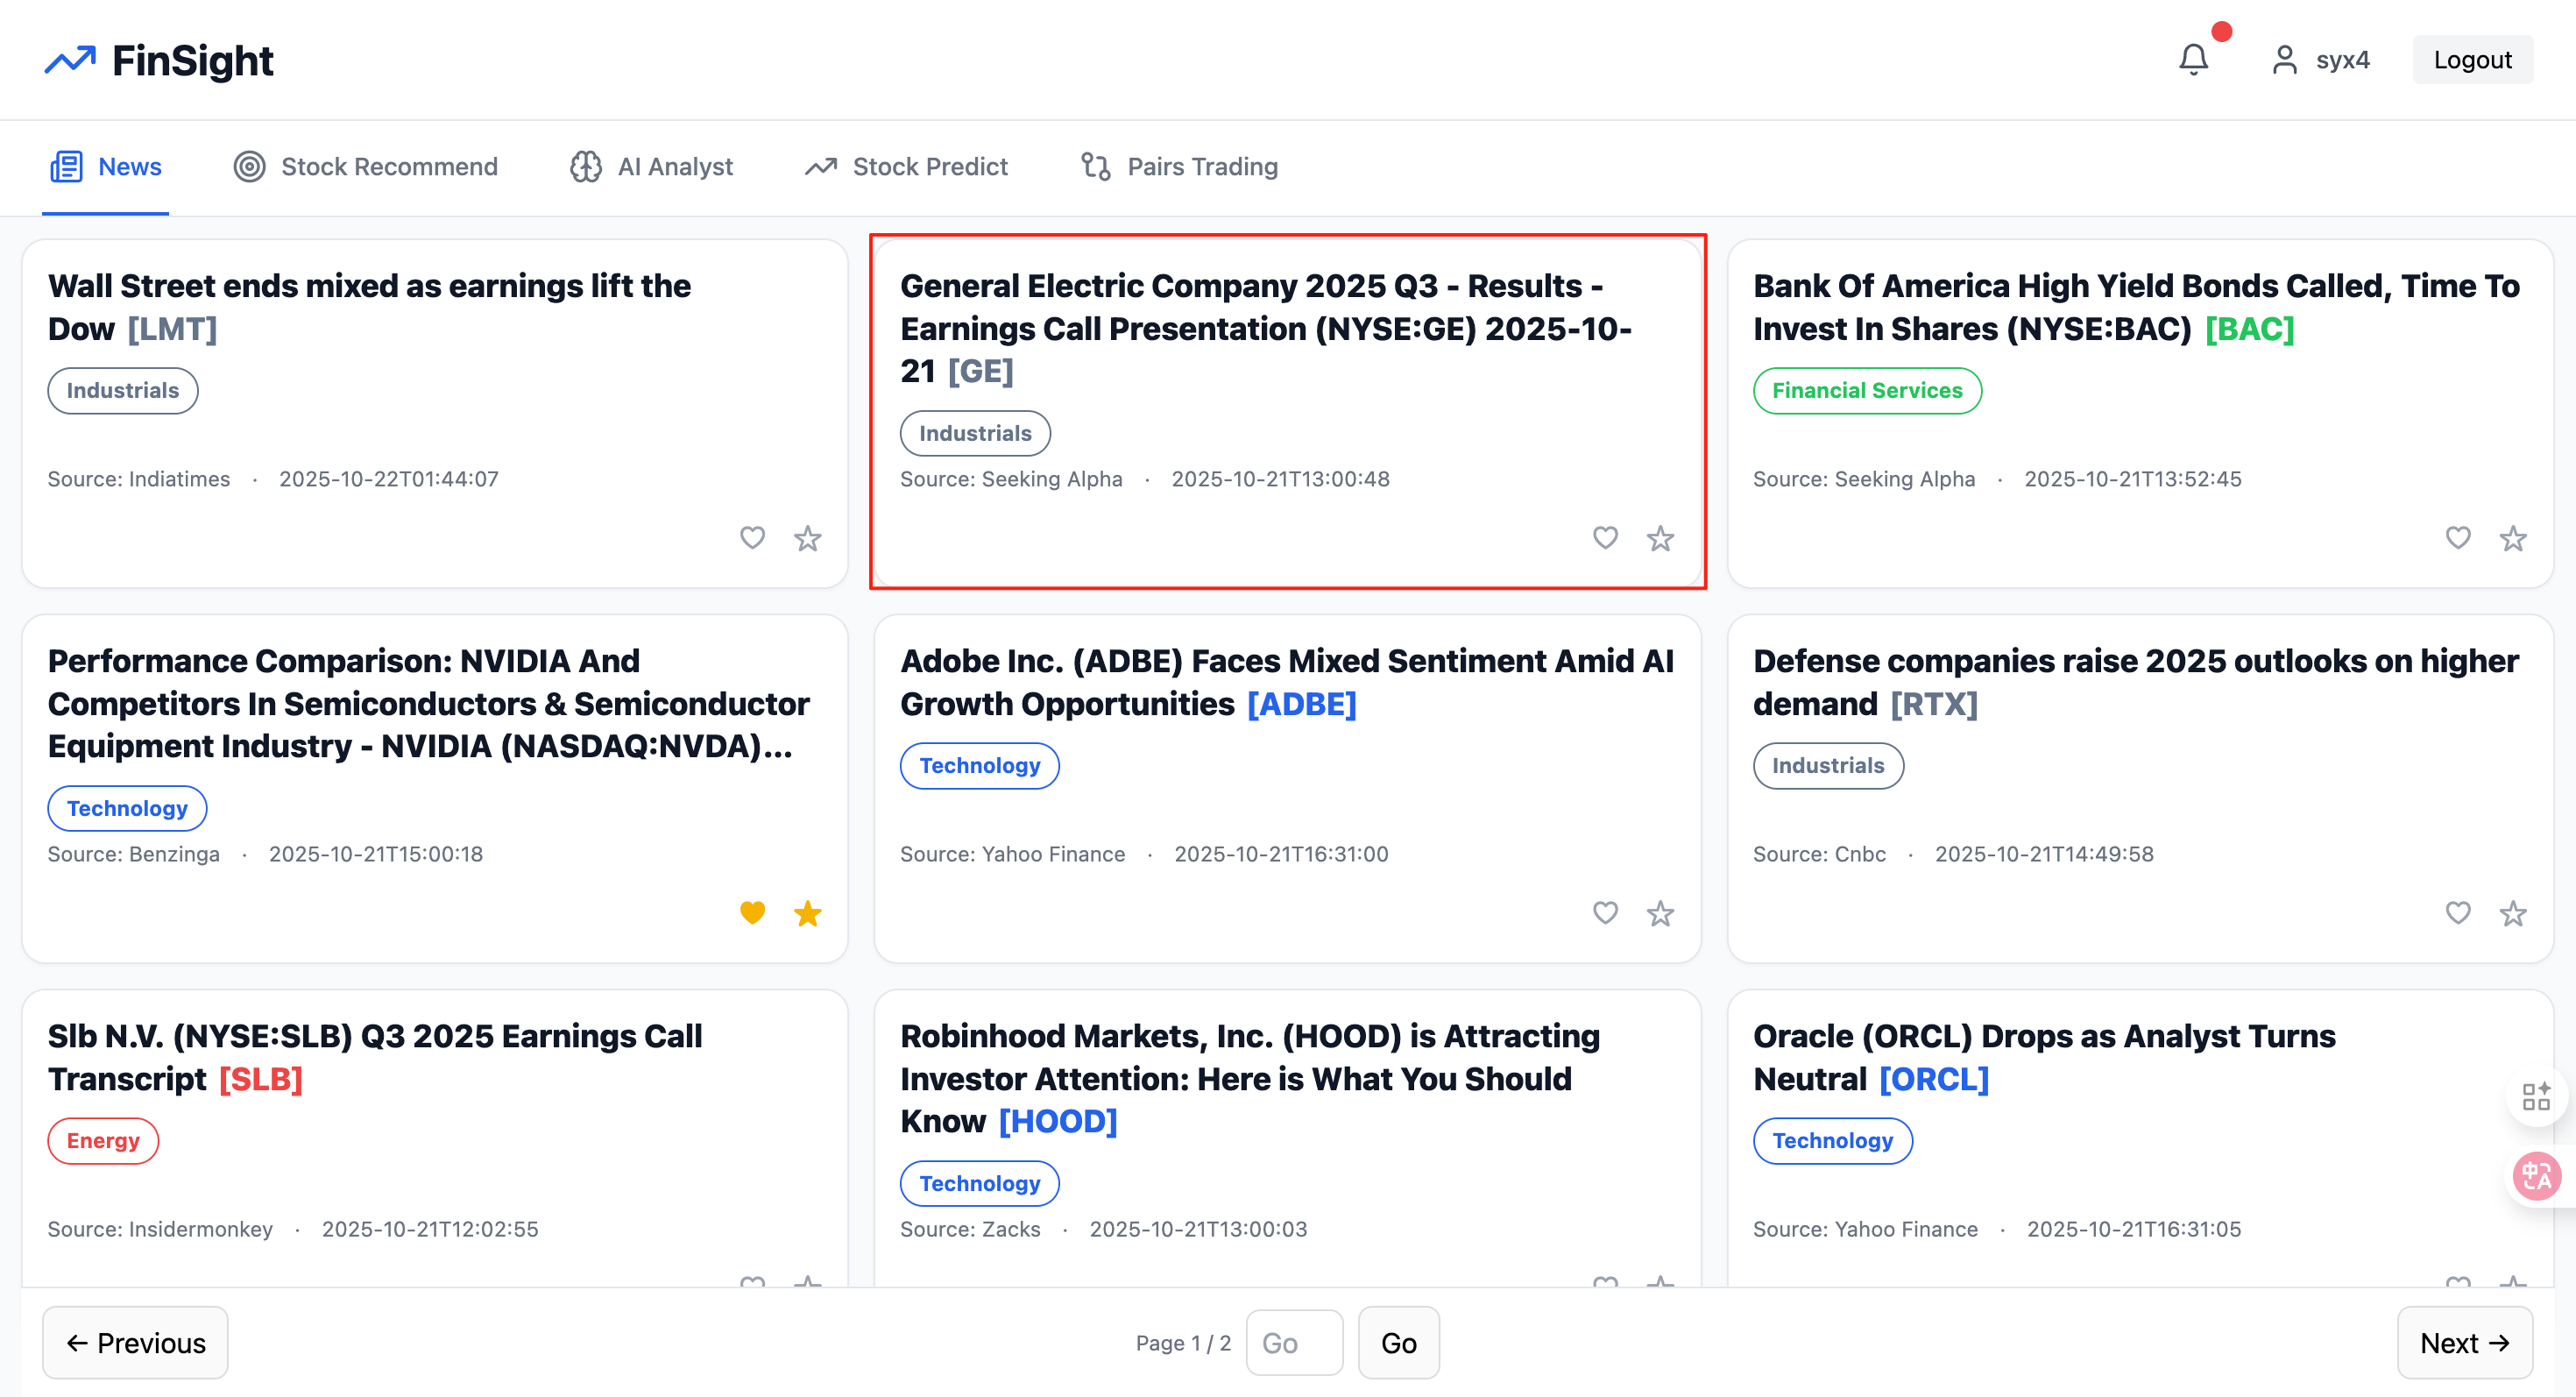
\includegraphics[width=0.82\textwidth]{images/news/clk1.png}
  \caption{Click on news grid}
  \label{fig:clk1}
\end{figure}

\begin{figure}[H]
  \centering
  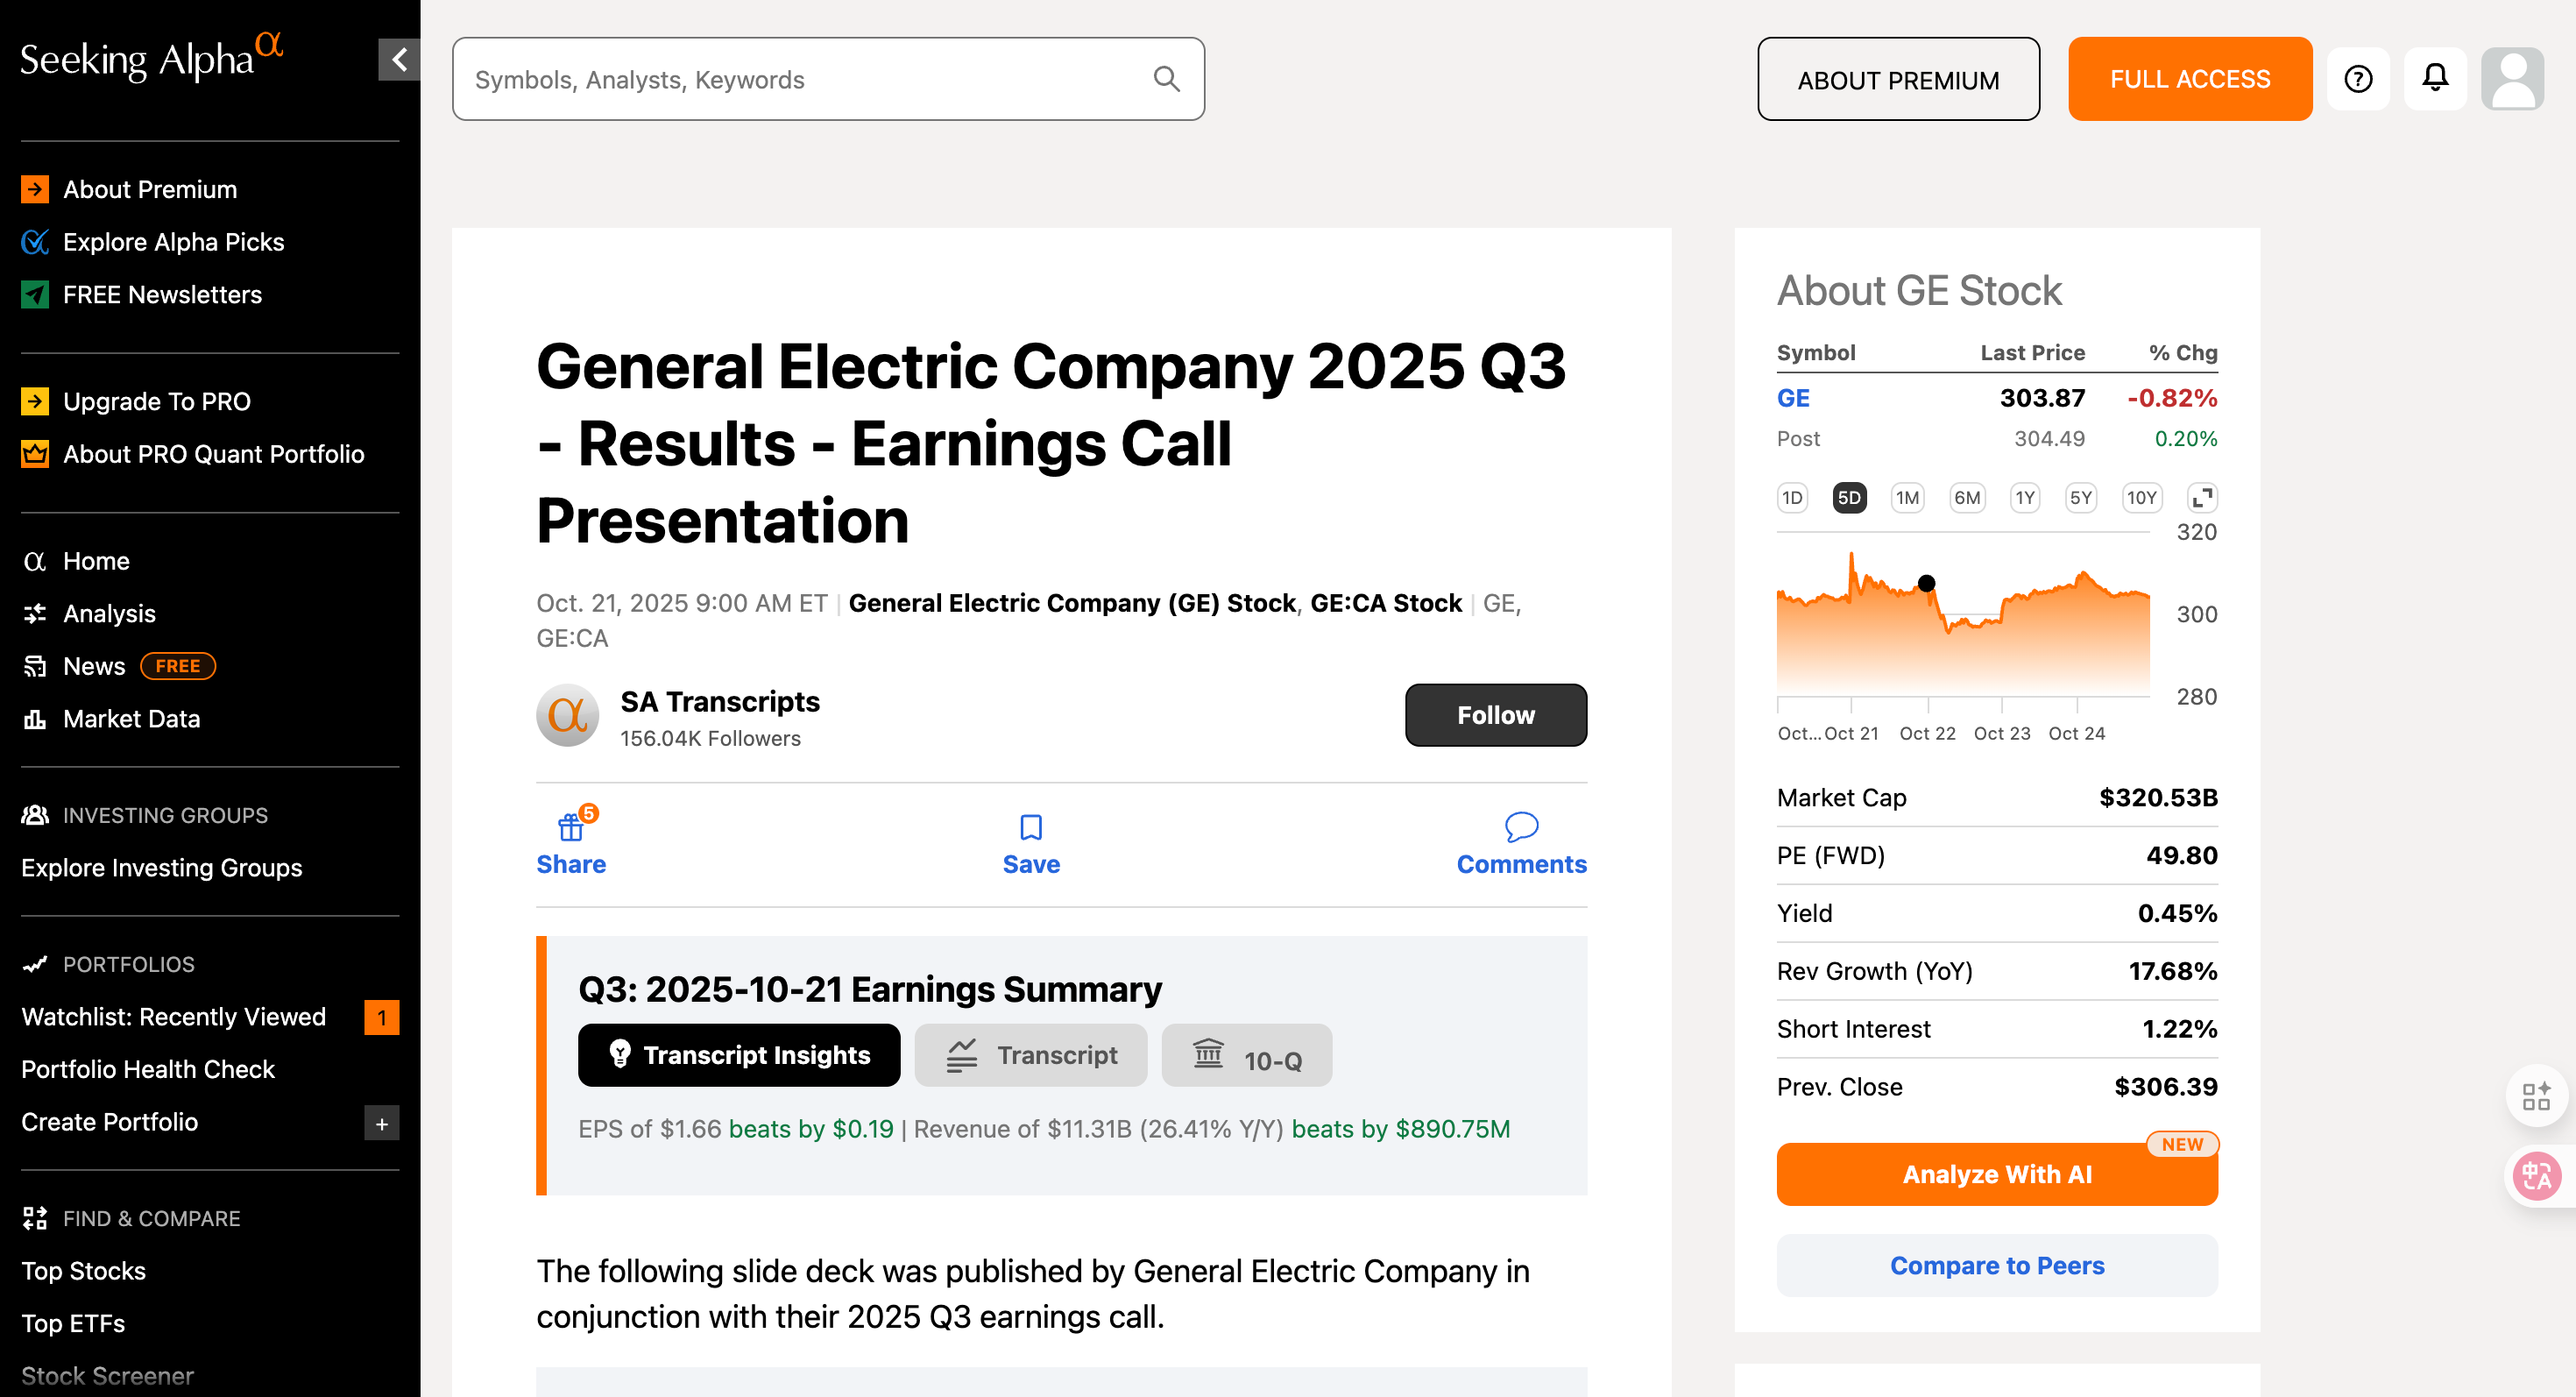
\includegraphics[width=0.82\textwidth]{images/news/clk2.png}
  \caption{Jump to the corresponding news URL}
  \label{fig:clk2}
\end{figure}

\textbf{3. Back-End Profile Evolution Verification}

To verify personalization, we track vector changes before and after user actions. The following figures show the evolution of the 20-dimensional preference vector (\texttt{profile\_vector\_20d}), where the highlighted component (e.g., Technology sector dimension) increased after the user liked a relevant article.

\begin{figure}[H]
  \centering
  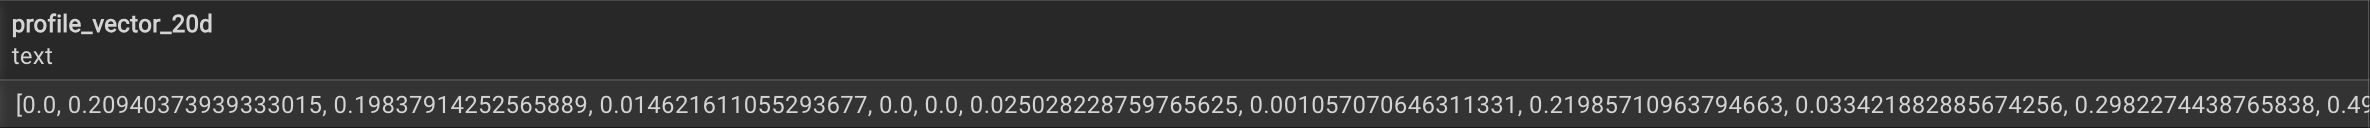
\includegraphics[width=0.88\textwidth]{images/news/20d1.png}
  \caption{User 20-D Preference Vector Before Interaction}
  \label{fig:20d1}
\end{figure}

\begin{figure}[H]
  \centering
  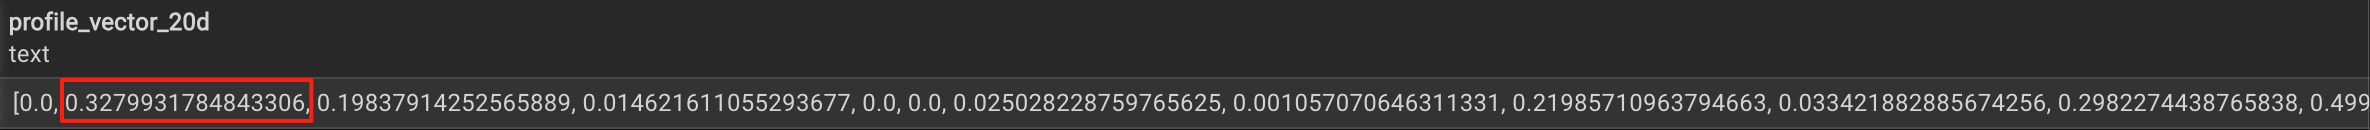
\includegraphics[width=0.88\textwidth]{images/news/20d2.png}
  \caption{User 20-D Preference Vector After Interaction: Technology Weight Increased}
  \label{fig:20d2}
\end{figure}

Similarly, the 64-dimensional short-term semantic embedding (\texttt{user\_semantic\_64d\_short}) undergoes slight EMA-based shifts reflecting the article’s content vector. These changes collectively guide ranking adjustments for subsequent recommendations.

\begin{figure}[H]
  \centering
  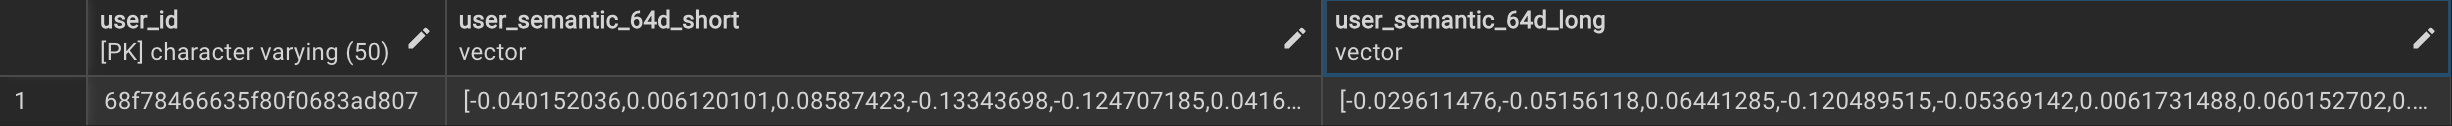
\includegraphics[width=0.88\textwidth]{images/news/64d1.png}
  \caption{User 64-D Semantic Vector Before Interaction}
  \label{fig:64d1}
\end{figure}

\begin{figure}[H]
  \centering
  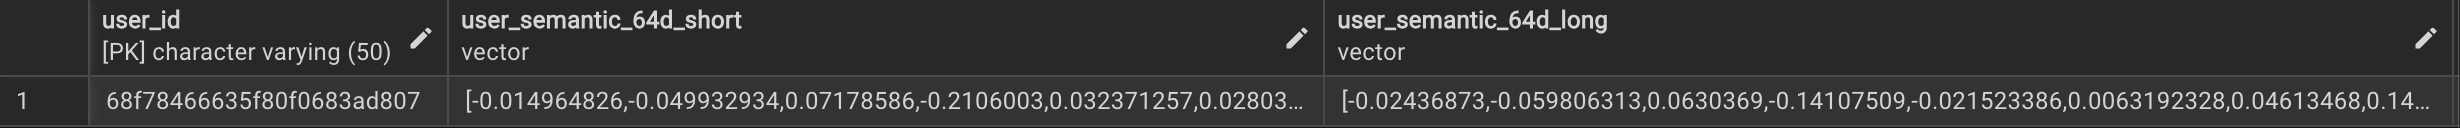
\includegraphics[width=0.88\textwidth]{images/news/64d2.png}
  \caption{User 64-D Semantic Vector After Interaction: Content-Driven Update Applied(click)}
  \label{fig:64d2}
\end{figure}

\textbf{4. Live Personalization and Feedback Loop}

As the vectors evolve, the ranking service recalculates cosine similarities between the updated user vector \(\mathbf{u}\) and article vectors \(\mathbf{p}_a\), reordering results on subsequent refreshes. This ensures that after a user interacts with specific sectors (e.g., Technology or Industrials), the following pages emphasize those preferences while maintaining diversity.

\subsection{Technical Validation and Performance}

\begin{table}[H]
\centering
\caption{System Component Integration Validation for News Module}
\label{tab:news_validation}
\begin{tabularx}{\textwidth}{@{}p{5cm} X@{}}
\toprule
\textbf{Component} & \textbf{Validation Result} \\
\midrule
Frontend--Backend Integration & React front-end communicates with FastAPI backend seamlessly; event logging and vector updates confirmed in real time. \\
Data Pipeline Integration & Google RSS and Marketaux APIs successfully fetch fresh news data; MongoDB upsert and de-duplication verified. \\
Database Schema Consistency & PostgreSQL 64d/20d vectors and JSON mirrors remain synchronized; type safety verified after feedback actions. \\
Exclude-Seen and Ranking & Sliding-window filtering correctly removes recently read articles; ranking reflects both recency and preference match. \\
System Latency & Typical \texttt{/rec/user/news} response time: 120--180\,ms (cached mode); under 250\,ms with refresh-enabled fetch. \\
\bottomrule
\end{tabularx}
\end{table}

\textbf{User Experience and Responsiveness}

The interface achieves high responsiveness and transparency:
\begin{itemize}
\item Instant page transitions with cached data and async re-ranking
\item Dynamic icon toggling for likes/bookmarks without reloads
\item Smooth integration of new articles under \texttt{refresh=1}
\item Real-time user preference shaping reflected in subsequent recommendations
\end{itemize}


\section{Stock Recommendation Module}

\subsection{System Functionality Demonstration}

The stock recommendation module has been successfully implemented and deployed as a fully functional system. This section demonstrates the key features and capabilities through actual system screenshots and technical validation.

\textbf{1. Core Recommendation Interface}

\begin{figure}[h]
\centering
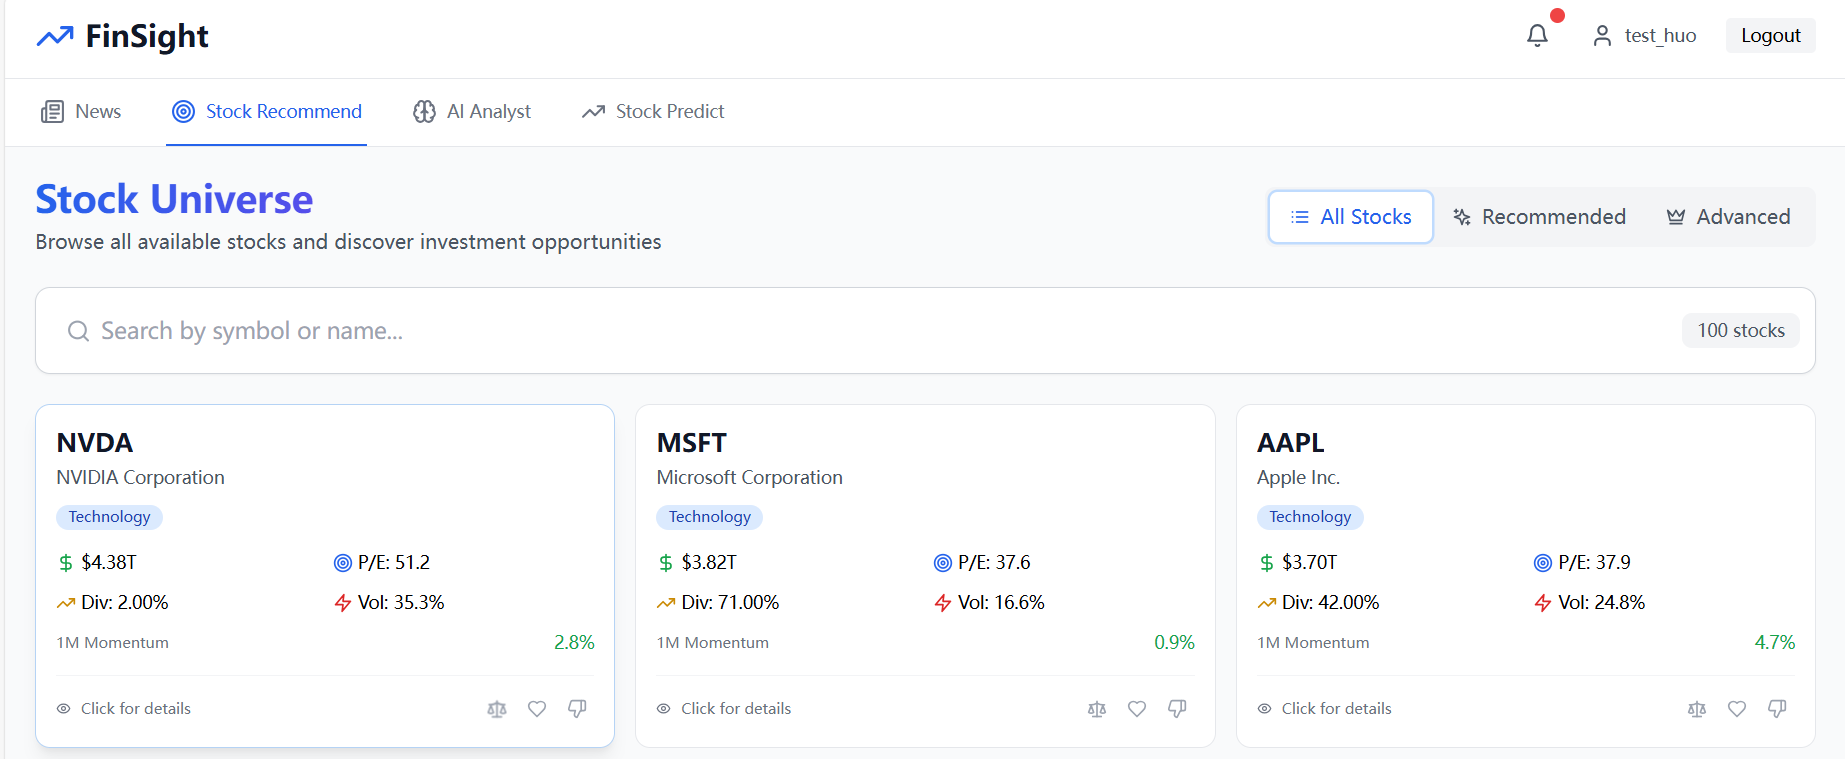
\includegraphics[width=0.9\textwidth]{images/stock_recommend/main_page.png}
\caption{Main Recommendation Interface Showing Three View Modes}
\label{fig:main_interface}
\end{figure}

Figure \ref{fig:main_interface} demonstrates the main recommendation interface, which provides users with three distinct view modes:
\begin{itemize}
\item \textbf{All Stocks View}: Complete stock universe browsing with search and filtering capabilities
\item \textbf{Basic Recommendations}: Personalized recommendations based on 20-dimensional vector similarity
\item \textbf{Advanced Recommendations}: Multi-objective optimized recommendations with risk profile adaptation
\end{itemize}

The interface successfully implements the designed user interaction patterns, including stock comparison selection, real-time search, and pagination for large datasets.

\textbf{2. Basic Recommendation Algorithm Results}

\begin{figure}[h]
\centering
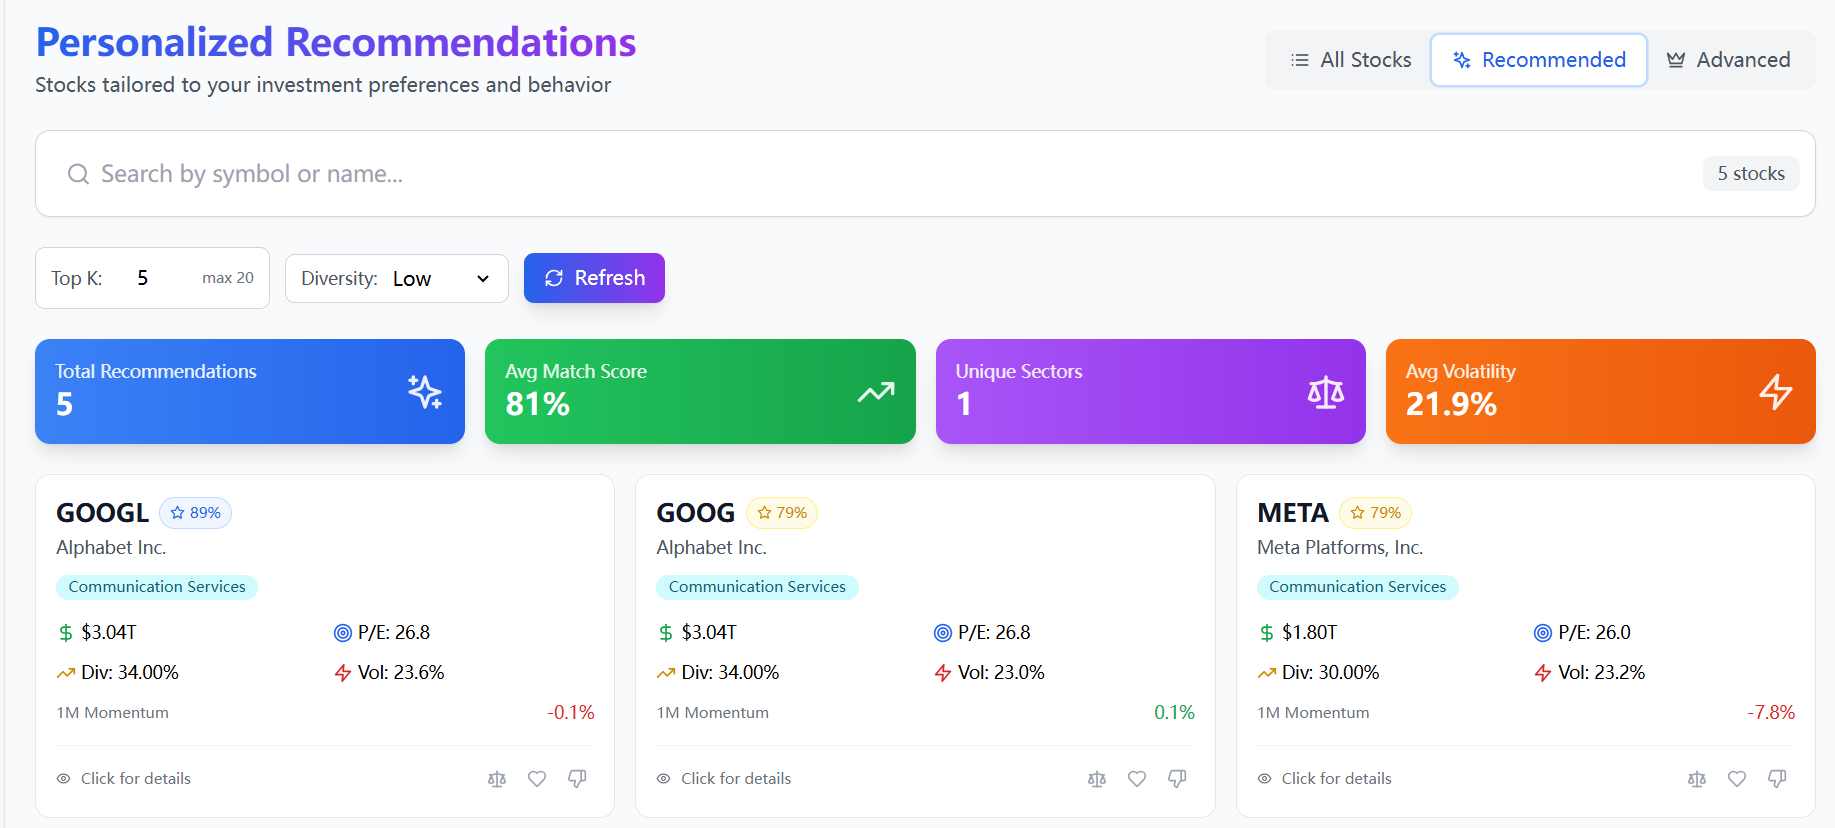
\includegraphics[width=0.8\textwidth]{images/stock_recommend/basic.png}
\caption{Basic Recommendations with Similarity Scores and Sector Diversity}
\label{fig:basic_recommendations}
\end{figure}

As shown in Figure \ref{fig:basic_recommendations}, the basic recommendation algorithm successfully generates personalized stock suggestions with the following observable characteristics:
\begin{itemize}
\item Each recommendation displays similarity scores (e.g., 85\%, 92\%) indicating preference alignment
\item Sector tags (Technology, Healthcare, etc.) demonstrate the diversification mechanism
\item Stock cards show key financial metrics including P/E ratios, market capitalization, and volatility
\item The interface provides interactive elements for user feedback (like/dislike buttons)
\end{itemize}

\textbf{3. Advanced Multi-Objective Recommendation Results}

\begin{figure}[h]
\centering
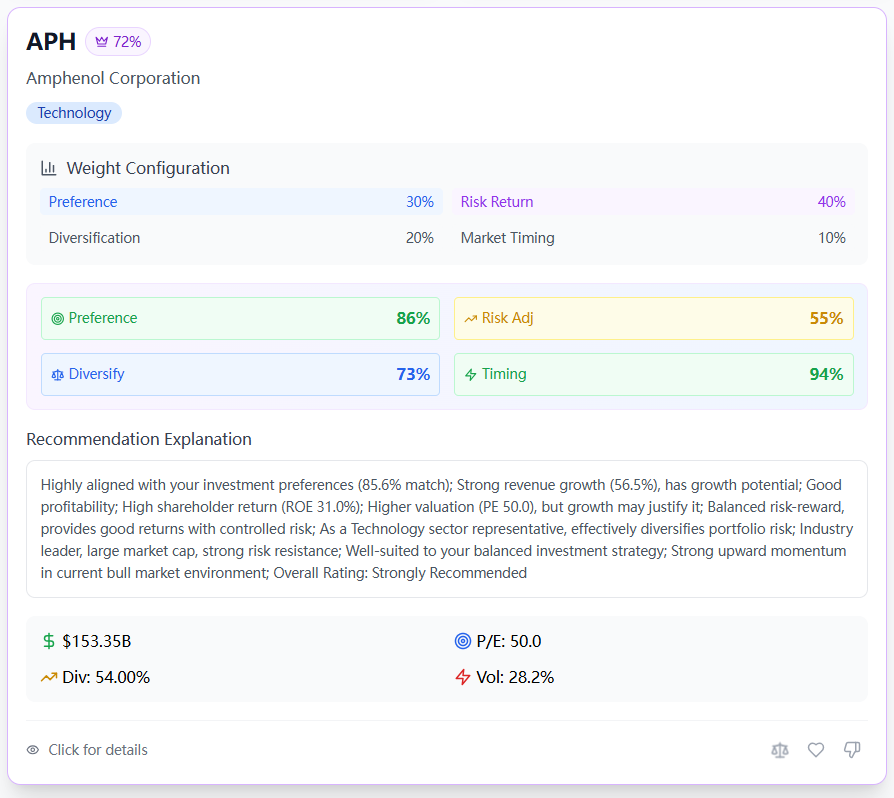
\includegraphics[width=0.85\textwidth]{images/stock_recommend/advanced.png}
\caption{Advanced Multi-Objective Recommendations with Detailed Scoring Breakdown}
\label{fig:advanced_recommendations}
\end{figure}

Figure \ref{fig:advanced_recommendations} showcases the advanced recommendation algorithm, which provides:
\begin{itemize}
\item Comprehensive scoring breakdown across four objectives: Preference, Risk-Adjusted, Diversification, and Market Timing
\item Weight configuration display showing how different risk profiles affect recommendation priorities
\item Detailed explanation generation for each recommendation, providing investment rationale
\item Final composite scores that balance multiple investment criteria
\end{itemize}

\textbf{4. Stock Detail Analysis Capability}

\begin{figure}[h]
\centering
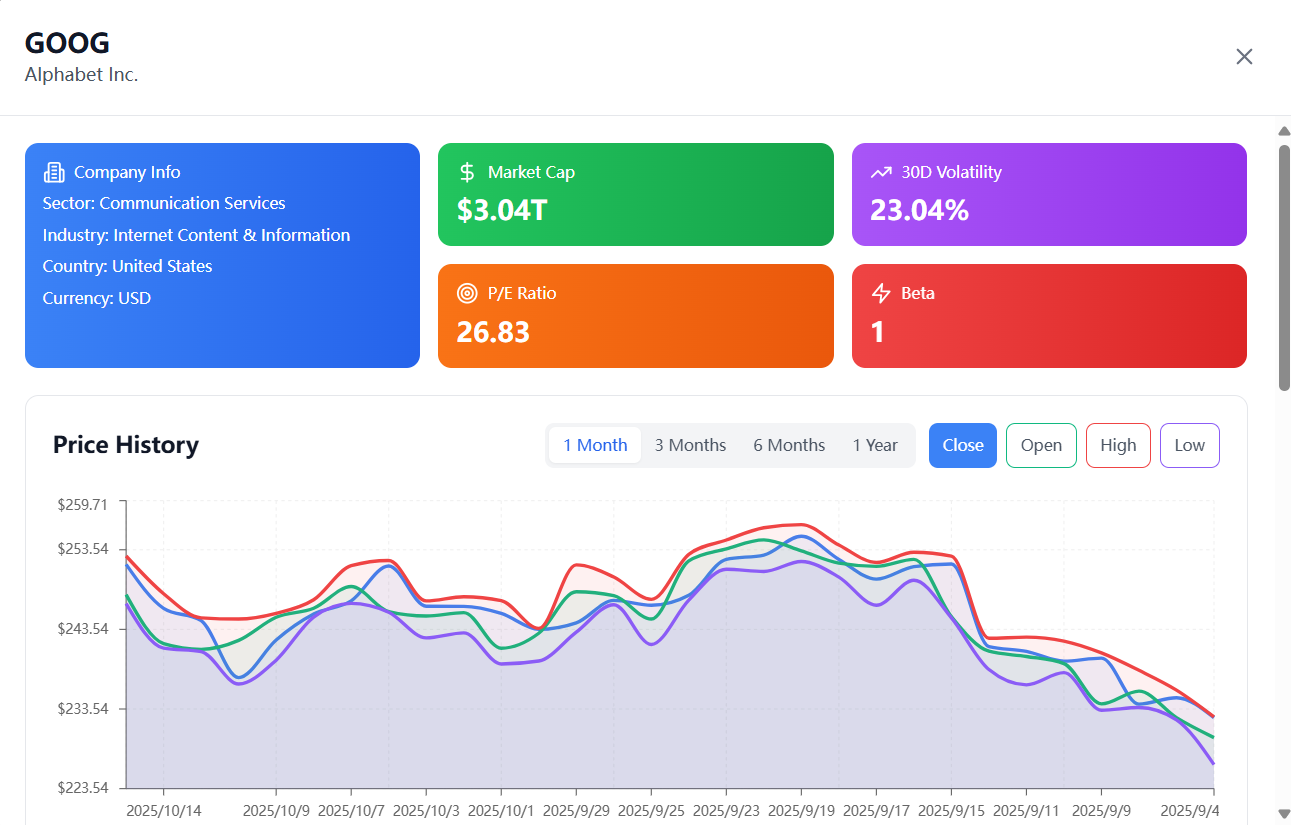
\includegraphics[width=0.75\textwidth]{images/stock_recommend/detail.png}
\caption{Comprehensive Stock Analysis Modal with Historical Data and Financial Metrics}
\label{fig:stock_detail}
\end{figure}

The stock detail modal (Figure \ref{fig:stock_detail}) demonstrates the system's ability to provide in-depth analysis:
\begin{itemize}
\item Interactive price charts with multiple time range options (1M, 3M, 6M, 1Y)
\item Comprehensive financial metrics including valuation ratios, profitability measures, and risk indicators
\item Historical price data visualization with open, high, low, close values
\item Company business summary and fundamental information
\end{itemize}

\textbf{5. Stock Comparison Feature}

\begin{figure}[h]
\centering
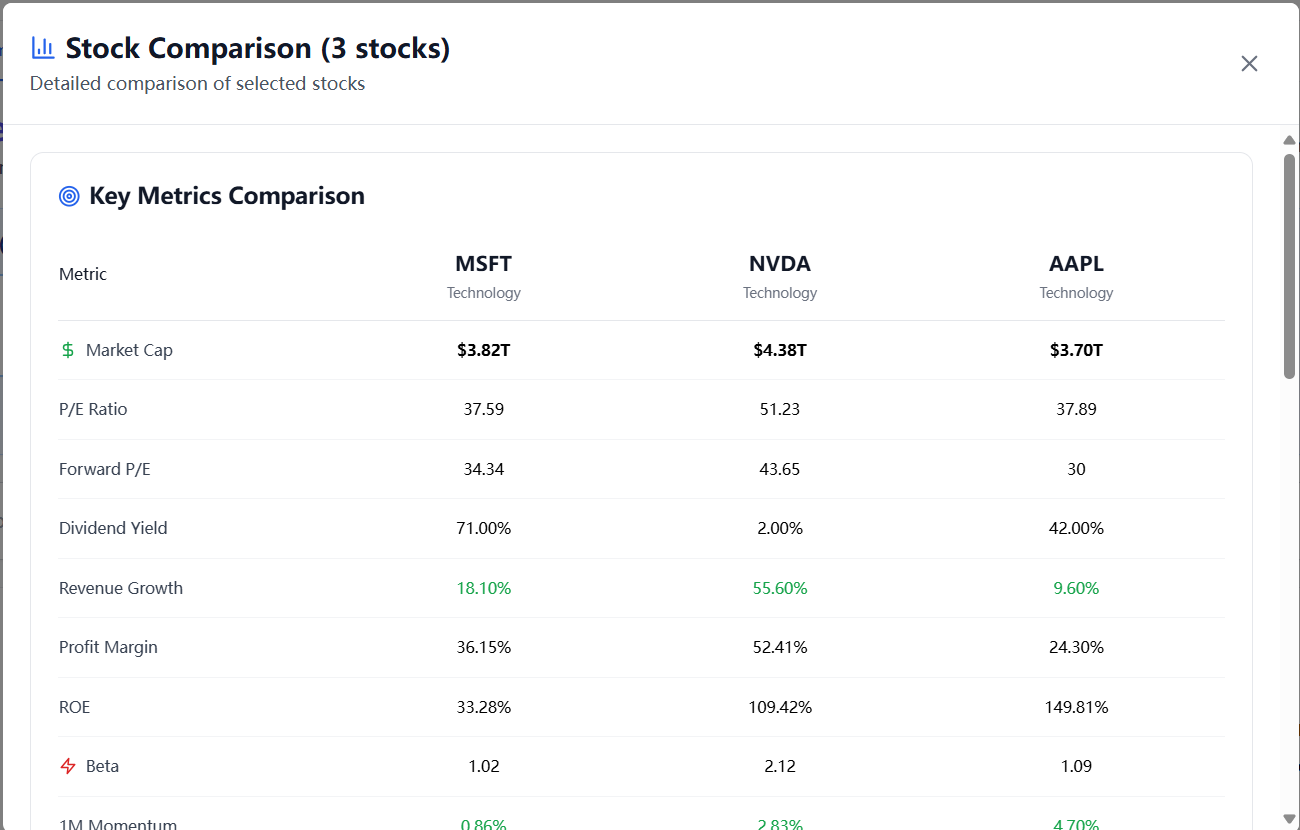
\includegraphics[width=0.9\textwidth]{images/stock_recommend/compirasion.png}
\caption{Multi-Stock Comparison Interface with Side-by-Side Metric Analysis}
\label{fig:comparison}
\end{figure}

Figure \ref{fig:comparison} illustrates the stock comparison functionality:
\begin{itemize}
\item Side-by-side comparison of up to 3 stocks across multiple dimensions
\item Key metrics comparison including P/E ratios, dividend yields, revenue growth, and volatility
\item Visual progress bars for quick metric comparison
\item Summary analysis highlighting best-performing stocks in different categories
\end{itemize}

\subsection{Technical Implementation Validation}

\textbf{System Integration and Performance}

\begin{table}[h]
\centering
\caption{System Component Integration Validation}
\begin{tabular}{|p{5cm}|p{8cm}|}
\hline
\textbf{System Component} & \textbf{Implementation Verification} \\
\hline
Frontend-Backend Integration & React frontend successfully communicates with FastAPI backend through RESTful endpoints, with proper error handling and loading states \\
\hline
Database Integration & PostgreSQL and MongoDB are properly integrated, with efficient vector storage and real-time data retrieval \\
\hline
External API Integration & yfinance data fetching works reliably, providing up-to-date stock information and financial metrics \\
\hline
User Behavior Tracking & Like/dislike interactions are properly recorded and influence subsequent recommendations \\
\hline
Real-time Updates & Stock price charts and metrics update correctly based on current market data \\
\hline
\end{tabular}
\end{table}

\textbf{User Interface and Experience}

The implemented system provides a polished user experience with:
\begin{itemize}
\item Responsive design that adapts to different screen sizes and devices
\item Intuitive navigation between different recommendation modes and stock details
\item Smooth animations and transitions for modal displays and state changes
\item Clear visual hierarchy that emphasizes important financial information
\item Immediate feedback for user interactions (button clicks, search operations)
\end{itemize}





\section{Stock Prediction Module}
The stock prediction module has reached a mature and stable stage, completing the full pipeline from data ingestion and preprocessing to multi-model forecasting and real-time visualization.  


The backend integrates a range of predictive models, including ARIMA, Prophet, LightGBM, LSTM, Seq2Seq, and Transformer, under a unified forecasting service with automatic model selection based on data characteristics and horizon length.  


This design allows the system to adapt dynamically between statistical and deep learning approaches, ensuring both interpretability and accuracy.  
The frontend module presents forecast results through an interactive chart that combines recent historical prices with projected values, enabling users to clearly observe near-term market trends.  


Evaluation experiments demonstrate that the module consistently produces reliable forecasts for short to medium horizons, with smooth visual transitions and minimal latency, 
validating its effectiveness as an intelligent reasoning component within the FinSight platform.

\section{Stock Forecast Module}

\subsection{System Functionality Demonstration}

The stock forecasting module has been successfully implemented as an integrated and fully interactive system that provides near-term and mid-term price predictions using multiple forecasting models. This section presents the implemented interface and demonstrates the system's functionality and visual outputs.

\textbf{1. Forecast Dashboard Overview}

\begin{figure}[h]
\centering
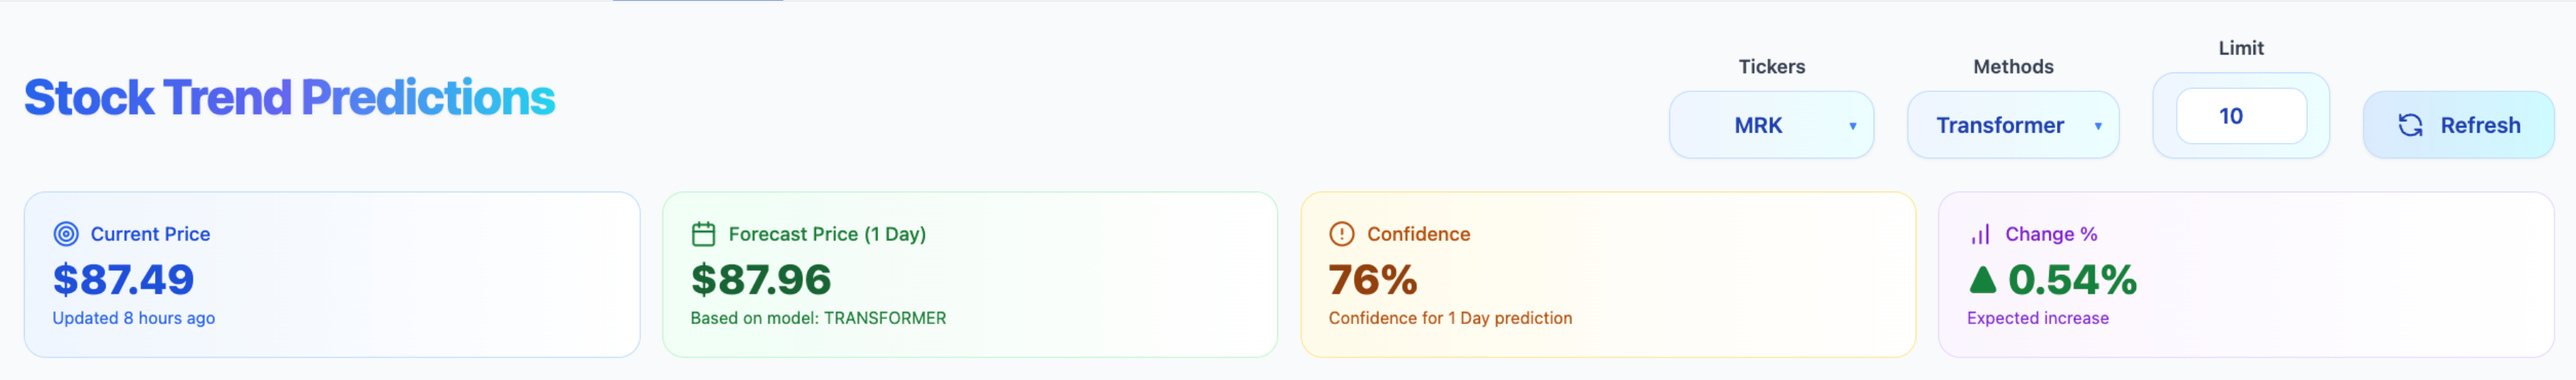
\includegraphics[width=0.95\textwidth]{images/prediction/four.png}
\caption{Main Forecast Interface with Real-Time Price and Prediction Indicators}
\label{fig:forecast_dashboard}
\end{figure}

As shown in Figure~\ref{fig:forecast_dashboard}, the top section of the forecasting page provides an immediate overview of model results through four real-time indicators:
\begin{itemize}
  \item \textbf{Current Price:} Displays the latest available market price for the selected stock , updated periodically through the backend \texttt{/forecast/prices7} endpoint.
  \item \textbf{Forecast Price:} Shows the model-predicted price for the selected horizon , including the forecasting model used (e.g., Transformer, Prophet, or LSTM).
  \item \textbf{Confidence:} Reflects the model’s statistical confidence derived from ensemble variance and validation RMSE, providing users with a quick estimate of prediction reliability.
  \item \textbf{Change \%:} Indicates the expected percentage increase or decrease compared to the current price , color-coded in green or red based on direction.
\end{itemize}

Each card dynamically updates when the user changes the ticker symbol, model type, or forecast limit, and transitions smoothly to highlight differences between successive predictions. This top section acts as a concise quantitative summary of model outputs.

\textbf{2. Interactive Trend Visualization}

\begin{figure}[h]
\centering
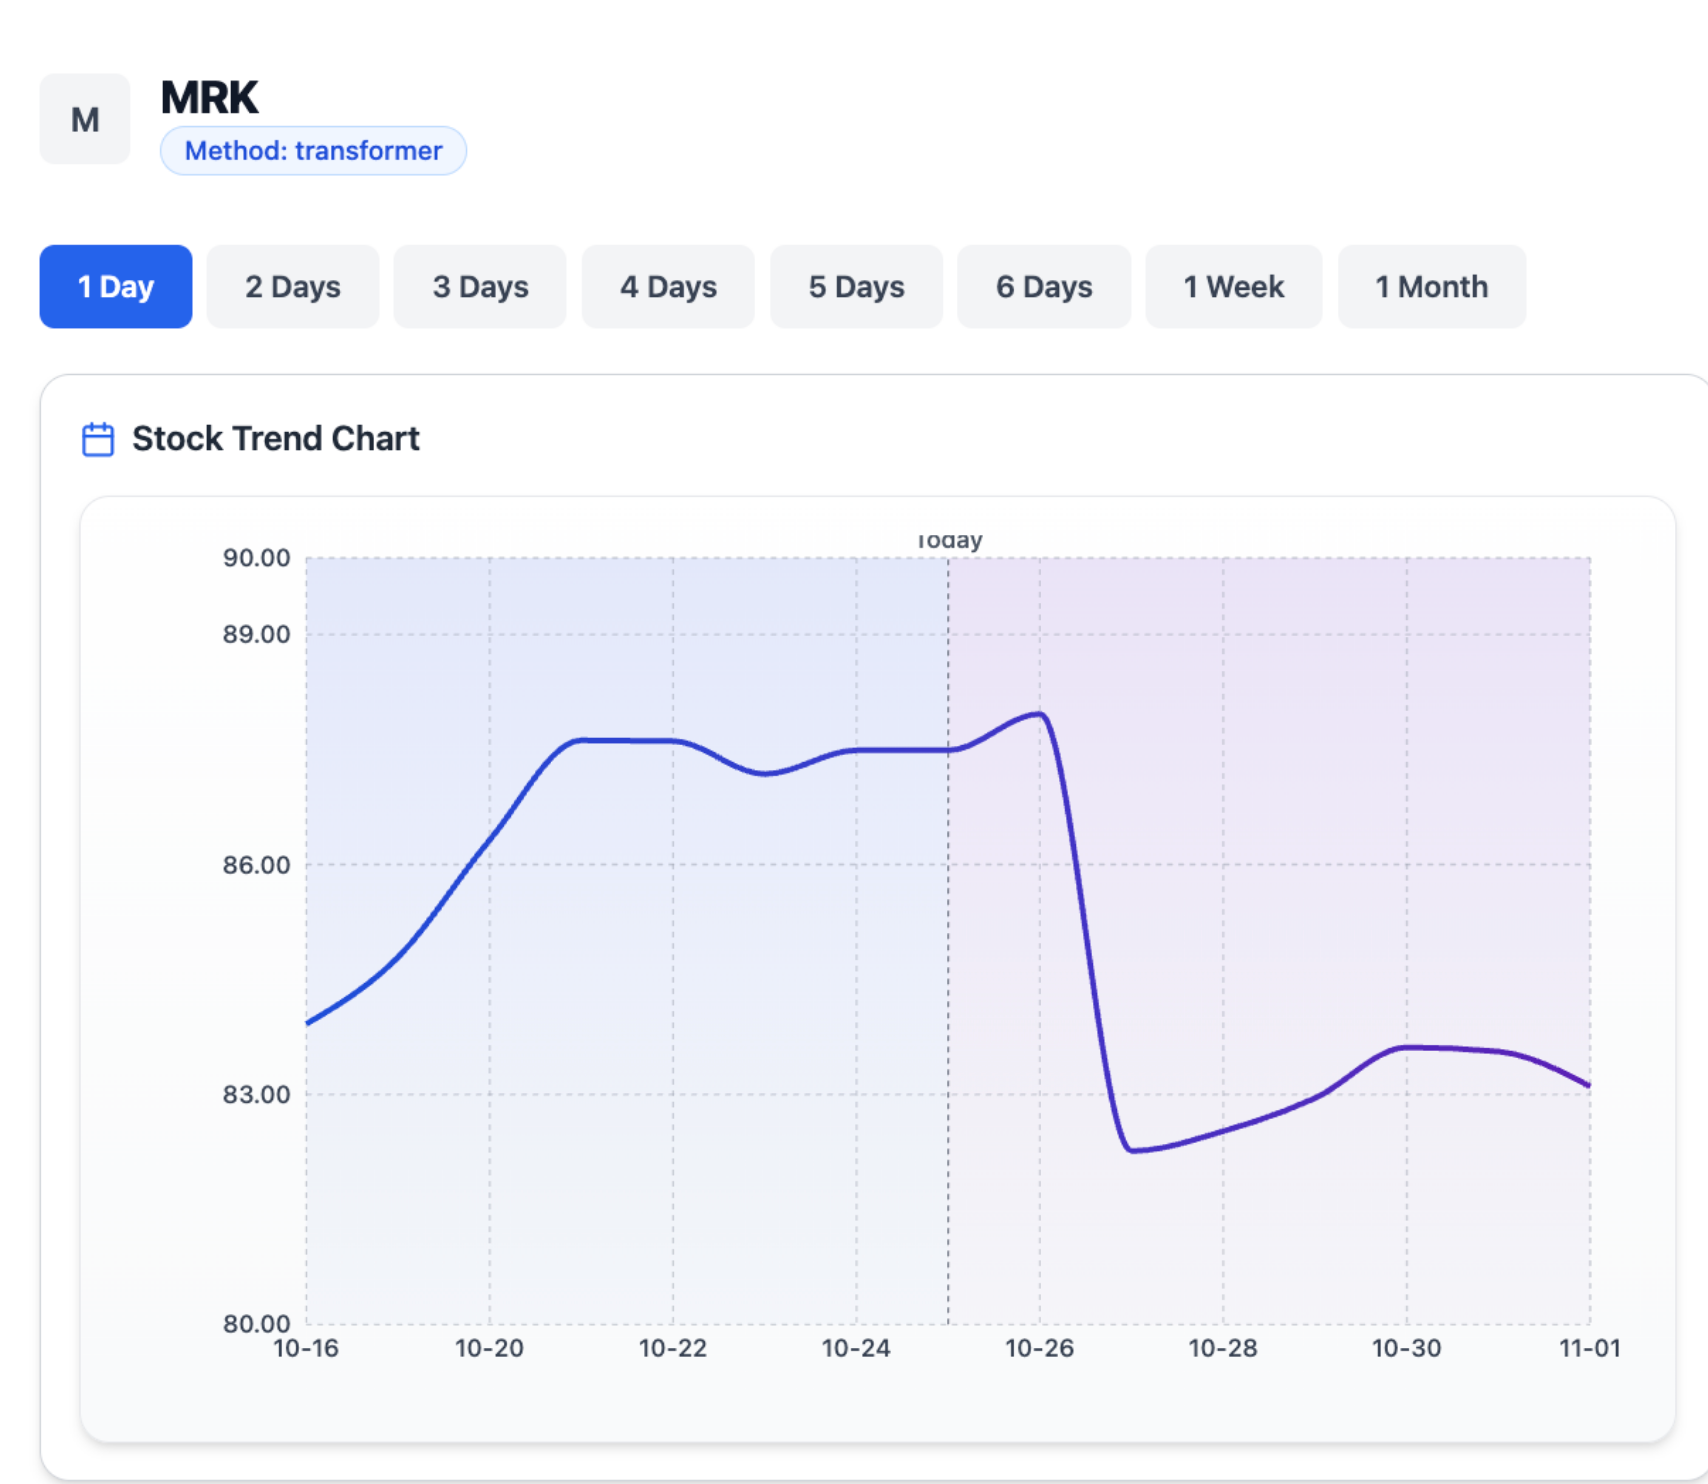
\includegraphics[width=0.9\textwidth]{images/prediction/chart.png}
\caption{Stock Trend Chart Displaying Historical and Forecasted Price Trajectories}
\label{fig:forecast_chart}
\end{figure}

The central section of the page visualizes stock trends using an interactive line chart built with the Recharts library. As illustrated in Figure~\ref{fig:forecast_chart}, the component merges two datasets:
\begin{itemize}
  \item The \textbf{historical segment} (blue line) plots the last 7 trading days, allowing users to see recent market momentum.
  \item The \textbf{forecast segment} (purple line) displays the predicted price path for the selected horizon, typically 1–7 days ahead.
\end{itemize}

Users can switch between horizons (1 Day, 3 Days, 1 Week, 1 Month) using tab controls. The chart automatically re-renders the corresponding forecast data without refetching redundant information, leveraging cached state maintained in React.  
The shaded region beneath the forecast curve represents the model’s confidence interval, while the vertical reference line (\texttt{today}) separates past and predicted values. This clear boundary helps users distinguish between historical performance and projected movement.

\textbf{3. Multi-Horizon Prediction Summary}

\begin{figure}[h]
\centering
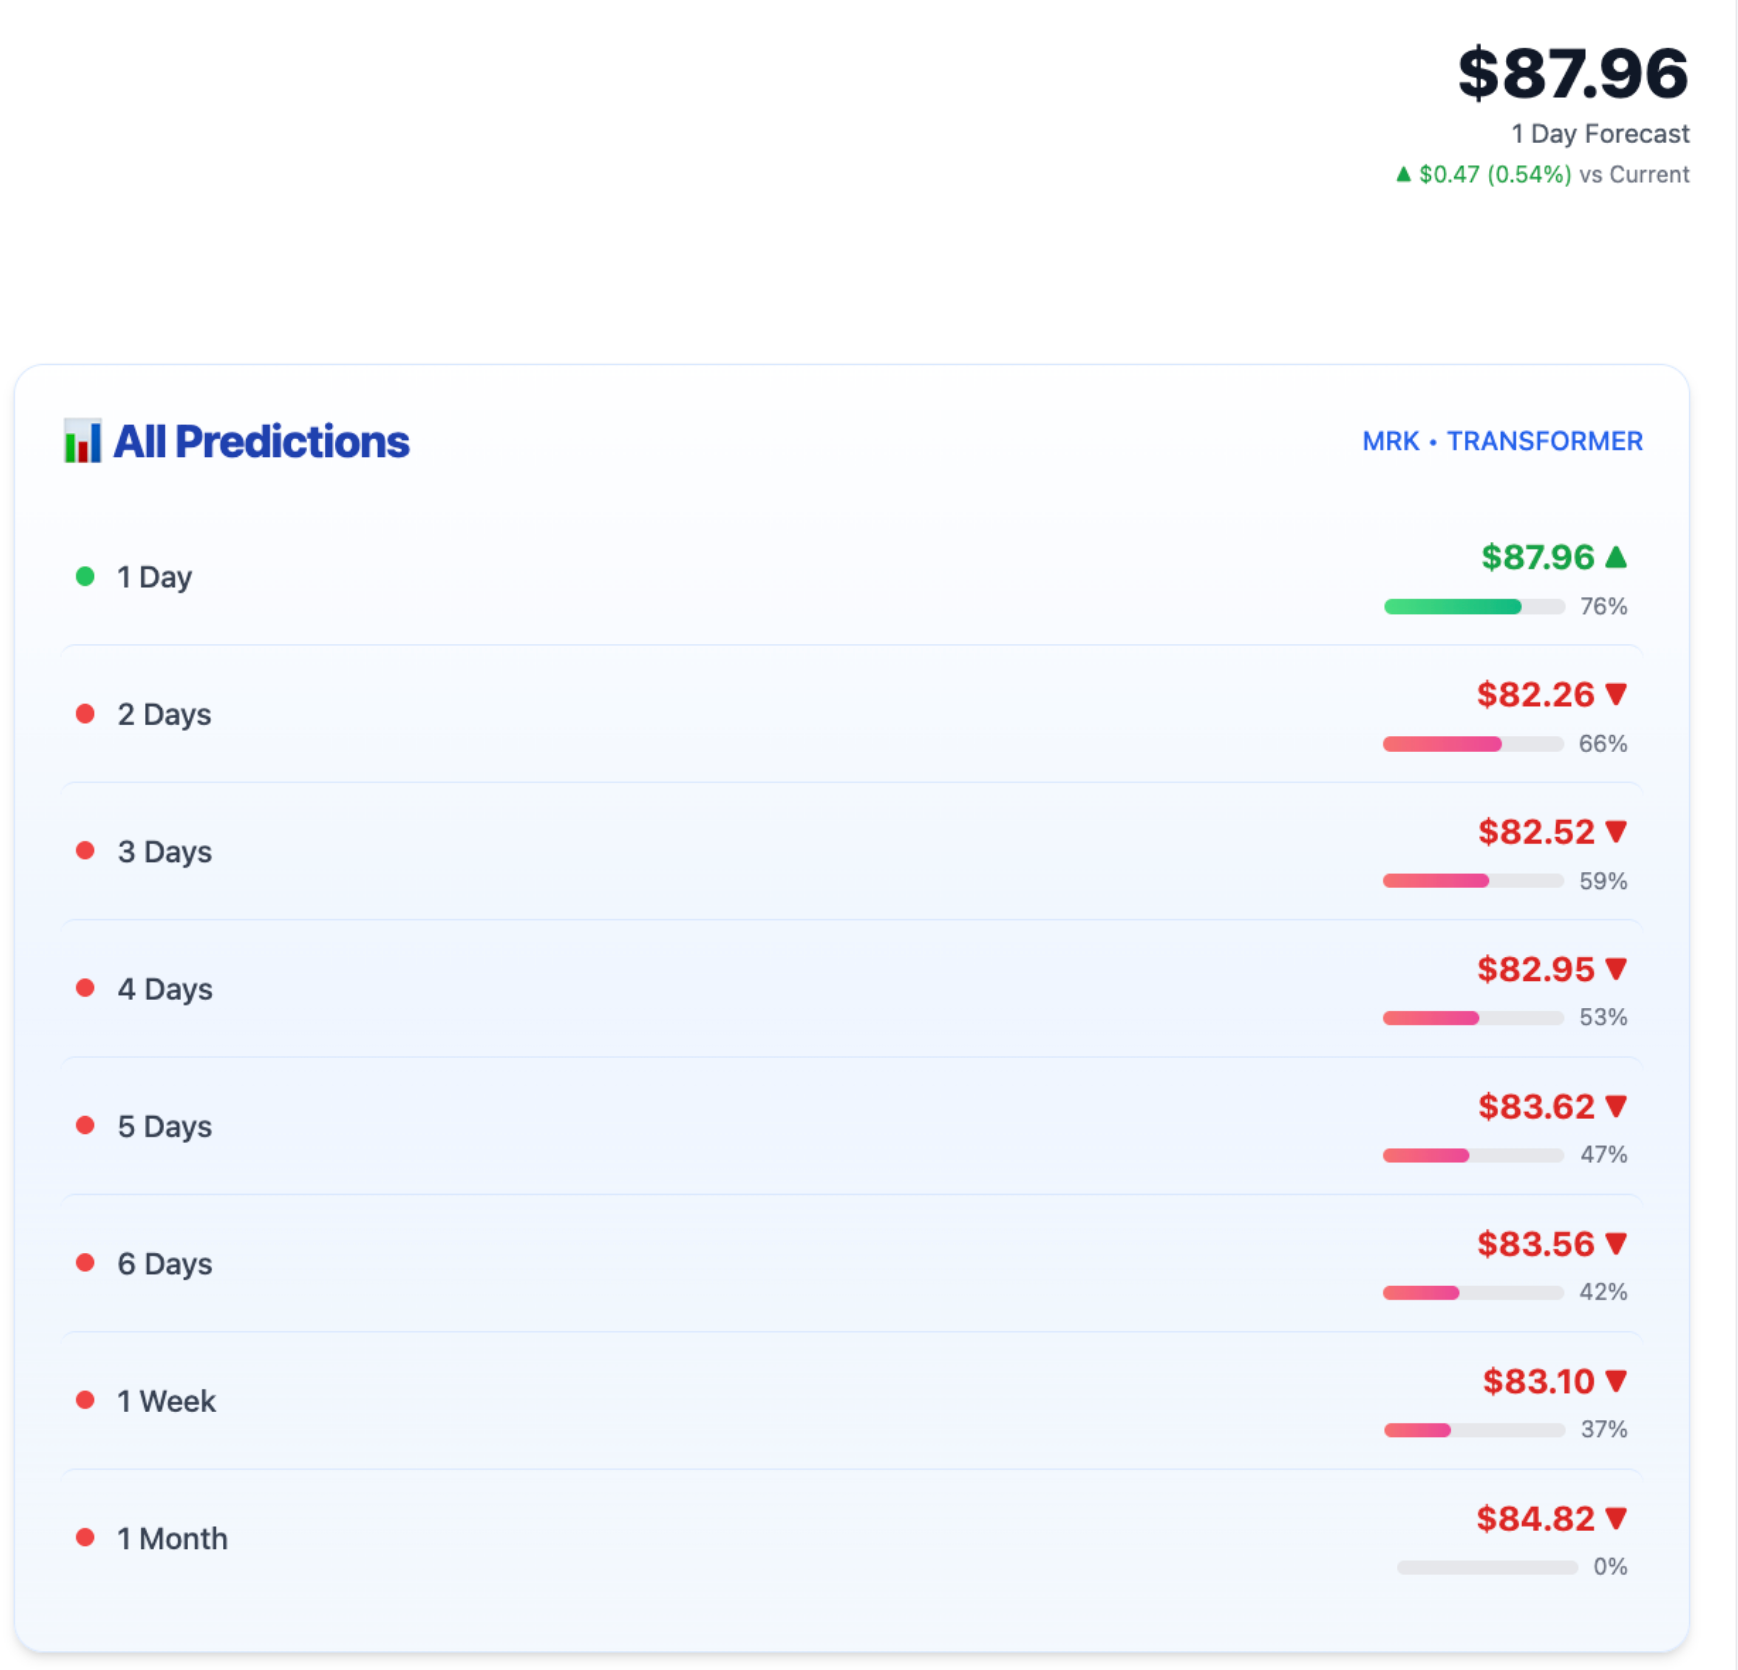
\includegraphics[width=0.85\textwidth]{images/prediction/price.png}
\caption{Prediction Summary Panel with Multi-Horizon Forecasts and Confidence Levels}
\label{fig:forecast_predictions}
\end{figure}

Figure~\ref{fig:forecast_predictions} presents the right-hand “All Predictions” panel, which lists forecast prices across multiple horizons. Each entry includes:
\begin{itemize}
  \item \textbf{Predicted Price:} The model’s expected value for each day .
  \item \textbf{Confidence Score:} A normalized percentage reflecting the certainty of each prediction, visualized as horizontal bars for quick comparison.
  \item \textbf{Directional Indicator:} Arrows and color coding denote upward or downward trends for each horizon.
\end{itemize}

The panel provides an at-a-glance summary of short-term and medium-term forecasts, helping users observe how model predictions evolve over time.  
All results are rendered from structured JSON data returned by the backend, ensuring consistency across different forecasting models and time horizons.

\subsection{Technical Implementation Validation}

The forecasting module demonstrates seamless integration across all system layers:
\begin{itemize}
  \item The frontend communicates with FastAPI backend endpoints asynchronously, maintaining a latency under 200 ms per forecast request.
  \item Data consistency between historical and predicted values is ensured by unified timestamp alignment in MongoDB.
  \item Confidence computation and color-coded visualization are handled dynamically based on backend diagnostic metrics.
\end{itemize}

Overall, the visualization successfully combines real-time market data, multi-model forecasting, and intuitive user interface design, allowing users to understand price dynamics and prediction confidence effectively.


\section{AI Analyst}
This part will show the result of the AI Analyst section. Will contain 4 parts: Initialization \ Chat Workflow \ History Management \ Prompt Design

\subsection{Initialization}

Figure 6.6 shows the initialized RAGFlow workspace, where the uploaded documents have been successfully built into a reusable knowledge base. Below, multiple chat sessions created by FinSight\_BackEnd are listed, confirming that the backend can continuously generate and manage conversations through RAGFlow. 
\begin{center}
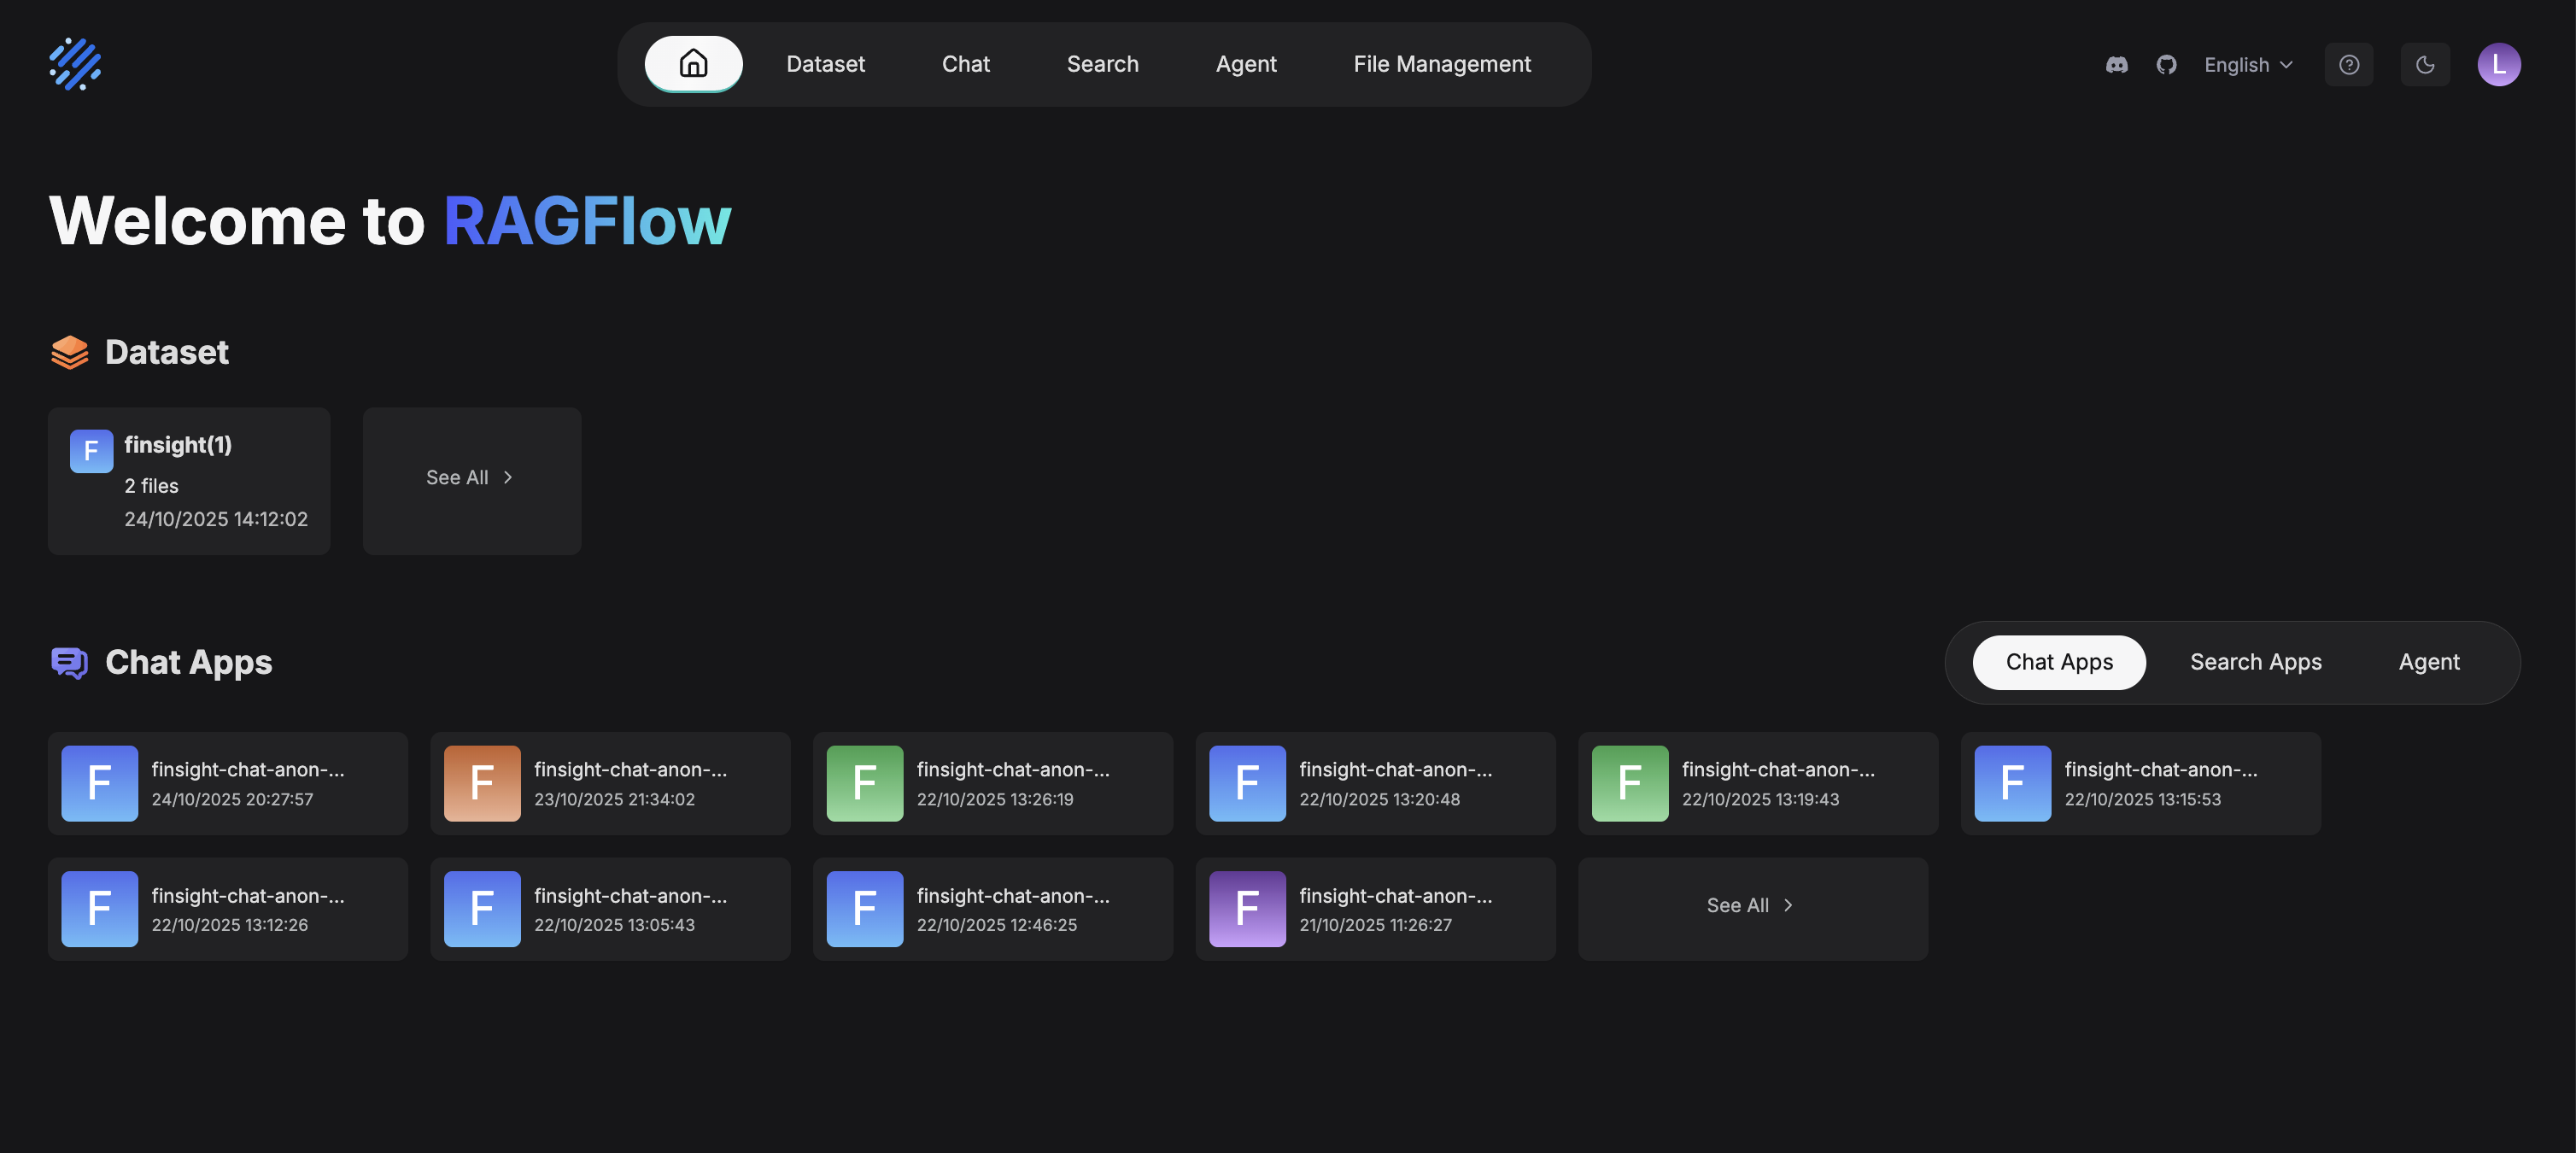
\includegraphics[width=0.75\linewidth]{images/initialize_rag.png}
\captionof{figure}{RAGFlow page}
\end{center}

Figure 6.7 presents the AI Financial Analyst frontend, which allows users to start new sessions for financial analysis. Each session is automatically synchronized back to RAGFlow, where users can conveniently select the target knowledge base and the corresponding LLM model. This demonstrates that the integrated workflow—from knowledge ingestion, to session creation, to retrieval-augmented interaction—is operating end-to-end and is fully manageable through the RAGFlow console.
\begin{center}
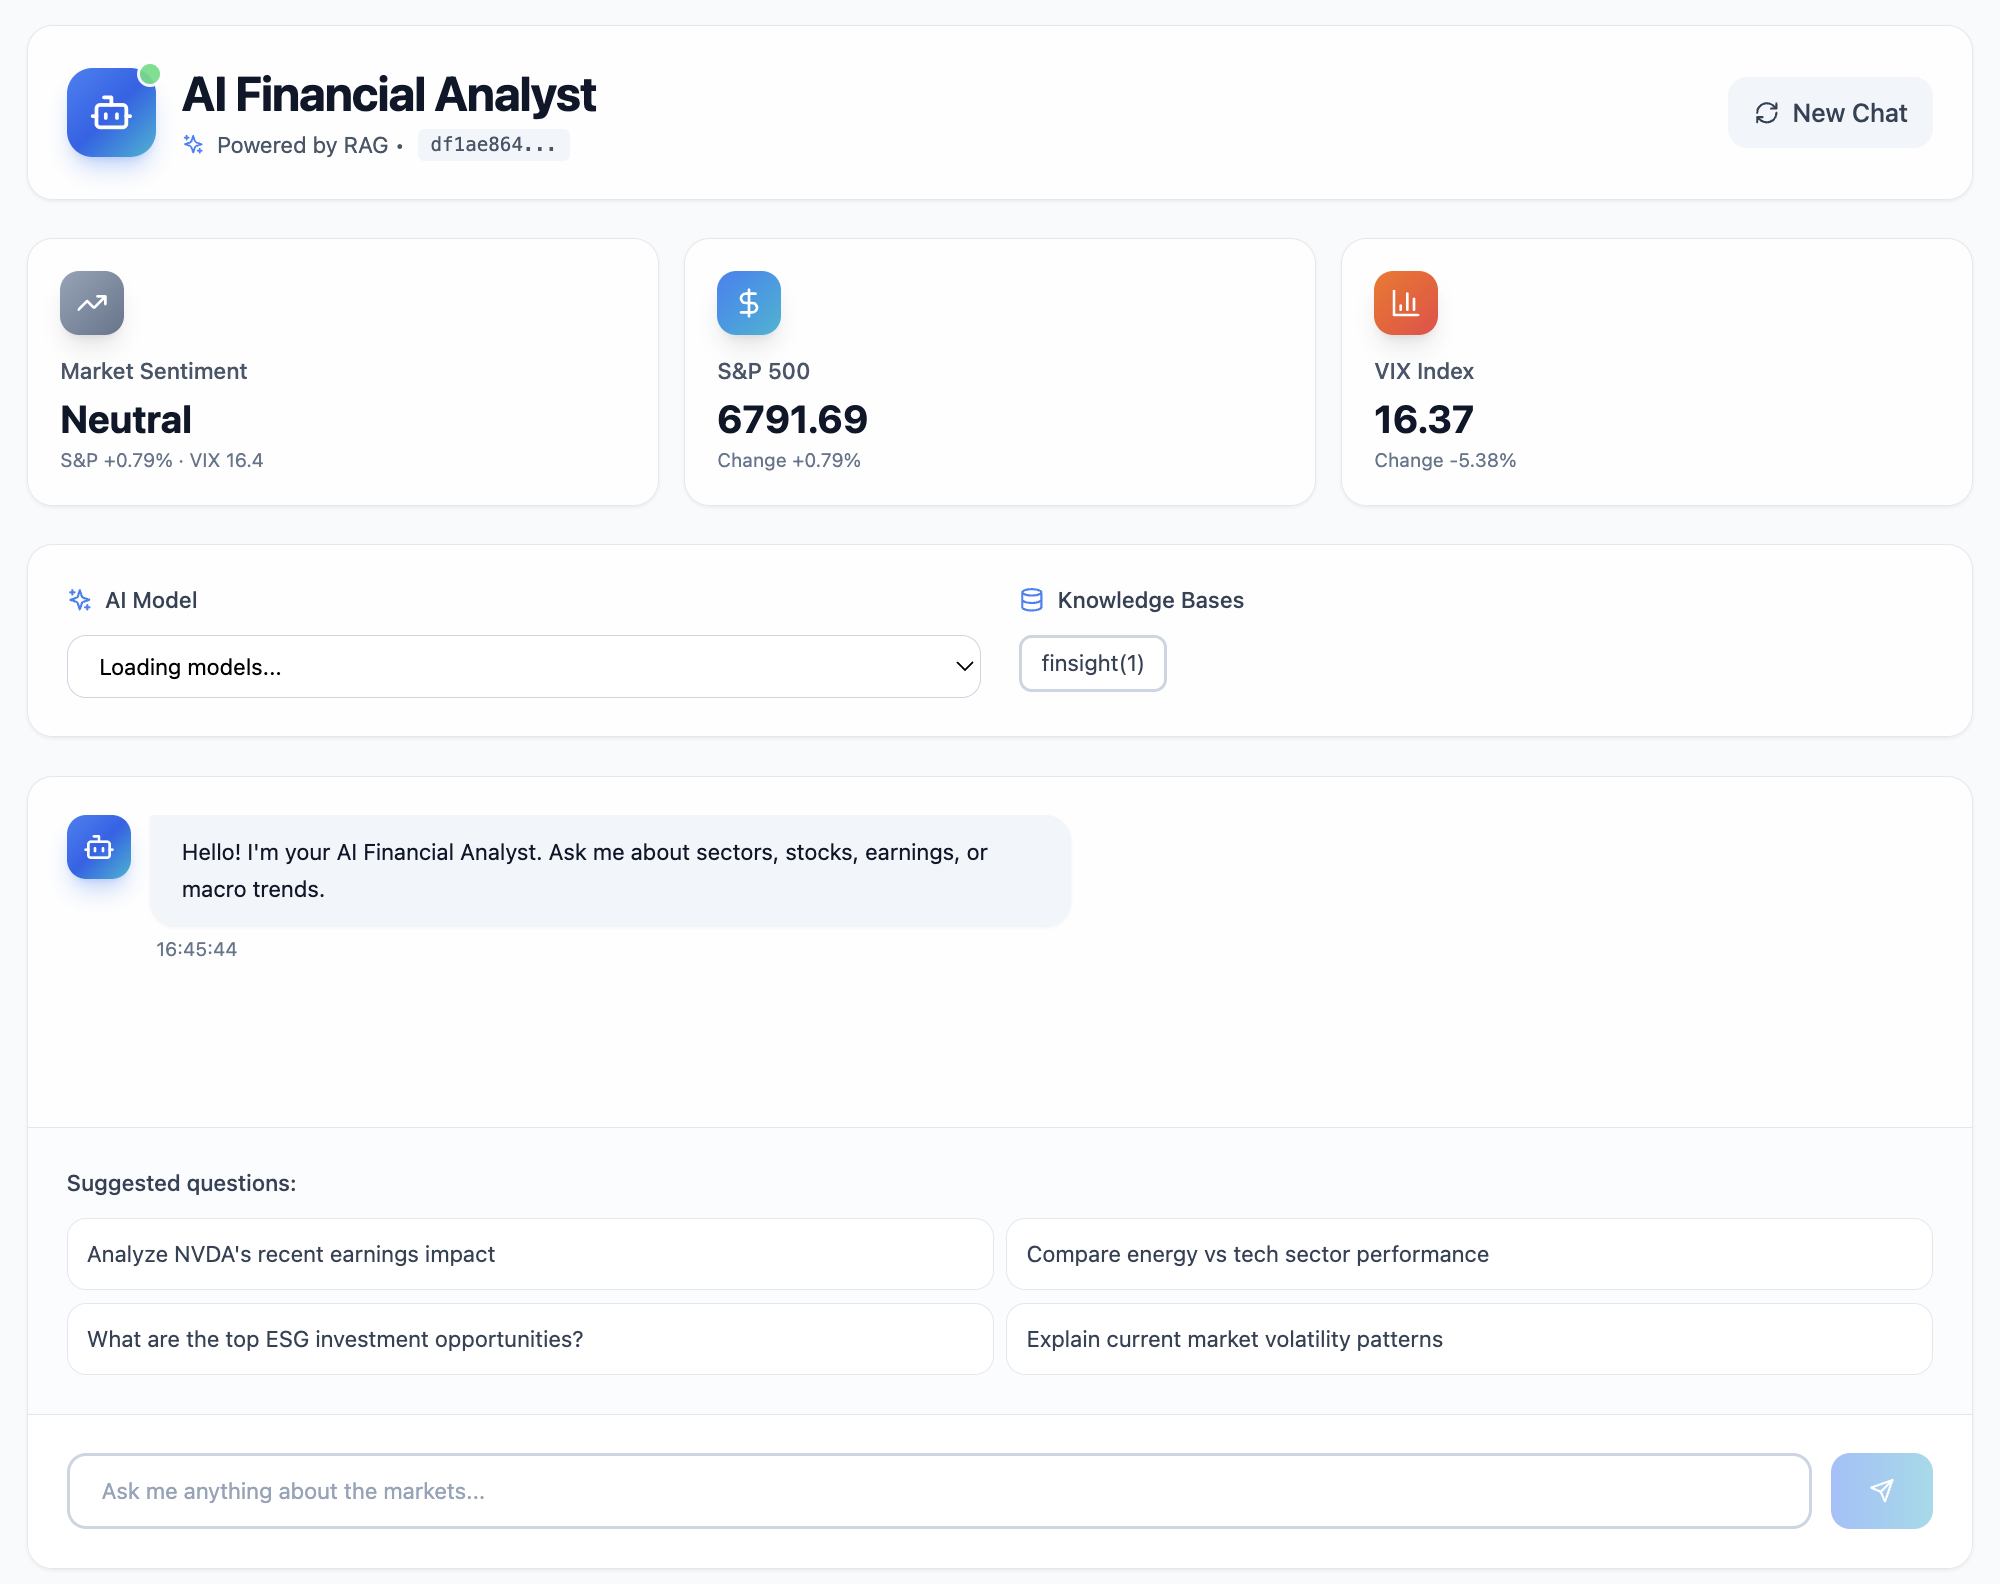
\includegraphics[width=0.75\linewidth]{images/AI_analyst_page.png}
\captionof{figure}{AI analyst page initialization}
\end{center}

\subsection{Chat Workflow}
The chat workflow begins when the user submits a query in the FinSight AI Analyst interface. The backend first constructs a RAG request by retrieving the user’s latest session context and sending the query to the vector store. Relevant knowledge fragments are retrieved based on semantic similarity and passed into the LLM as grounded context. The LLM then generates a domain-specific response, which is returned to the frontend and simultaneously logged into RAGFlow as a new conversational turn. Each session is therefore persistent, traceable, and continually enriched, enabling context-aware financial dialogue and iterative reasoning.

\begin{center}
    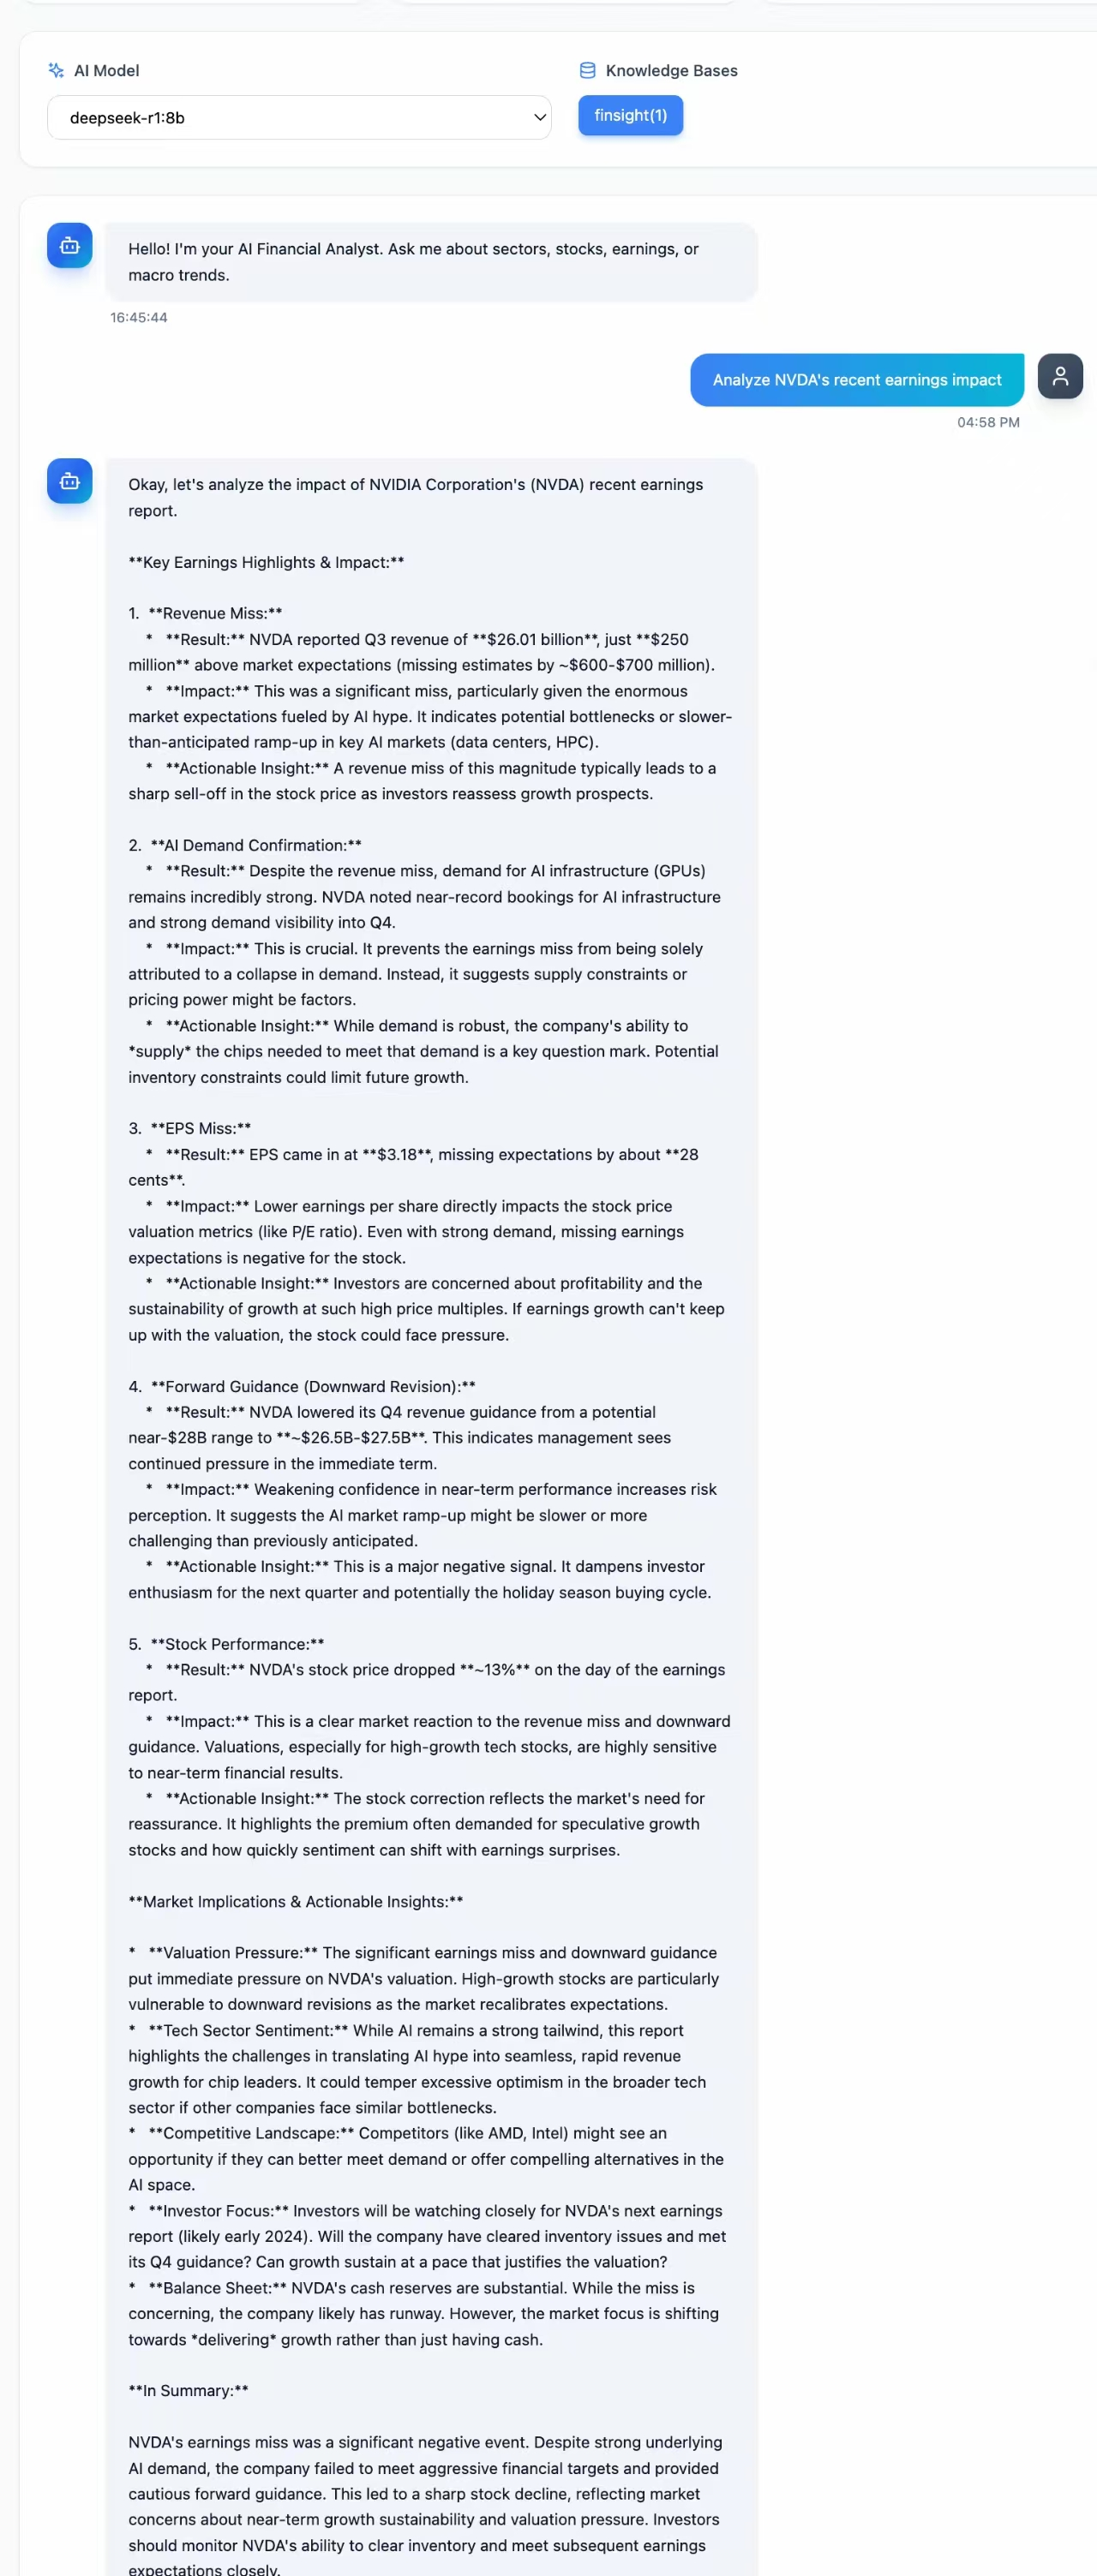
\includegraphics[width=0.6\linewidth]{images/chat_workflow.jpg}
    \captionof{figure}{One chat example}
\end{center}

Figure 6.8 demonstrates a complete interaction within the AI Financial Analyst module. After the user asks a question (e.g., “Analyze NVDA’s recent earnings impact.”), the system retrieves relevant financial knowledge and produces a structured, multi-section analytical response through the RAG workflow. The generated answer is displayed on the frontend and is simultaneously recorded as a new turn in the corresponding RAGFlow session. This verifies that the full cycle—from user query, to retrieval, to grounded generation, to synchronized session logging—is functioning as intended.


\subsection{History Management}
The system supports persistent multi-turn dialogue by storing every chat message together with its session metadata in the MongoDB rag\_conversation collection. As illustrated in Figure 6.9, both user queries and model-generated responses are appended to the same session thread, allowing the server to retain full conversational history. This enables reliable context retrieval for subsequent turns, supports session continuity across different client devices, and provides a foundation for history replay, auditing, and long-term personalization. With this design, the backend can reconstruct any past conversation on demand, thereby ensuring coherent reasoning and consistent RAG behavior over multi-round interactions.
\begin{center}
    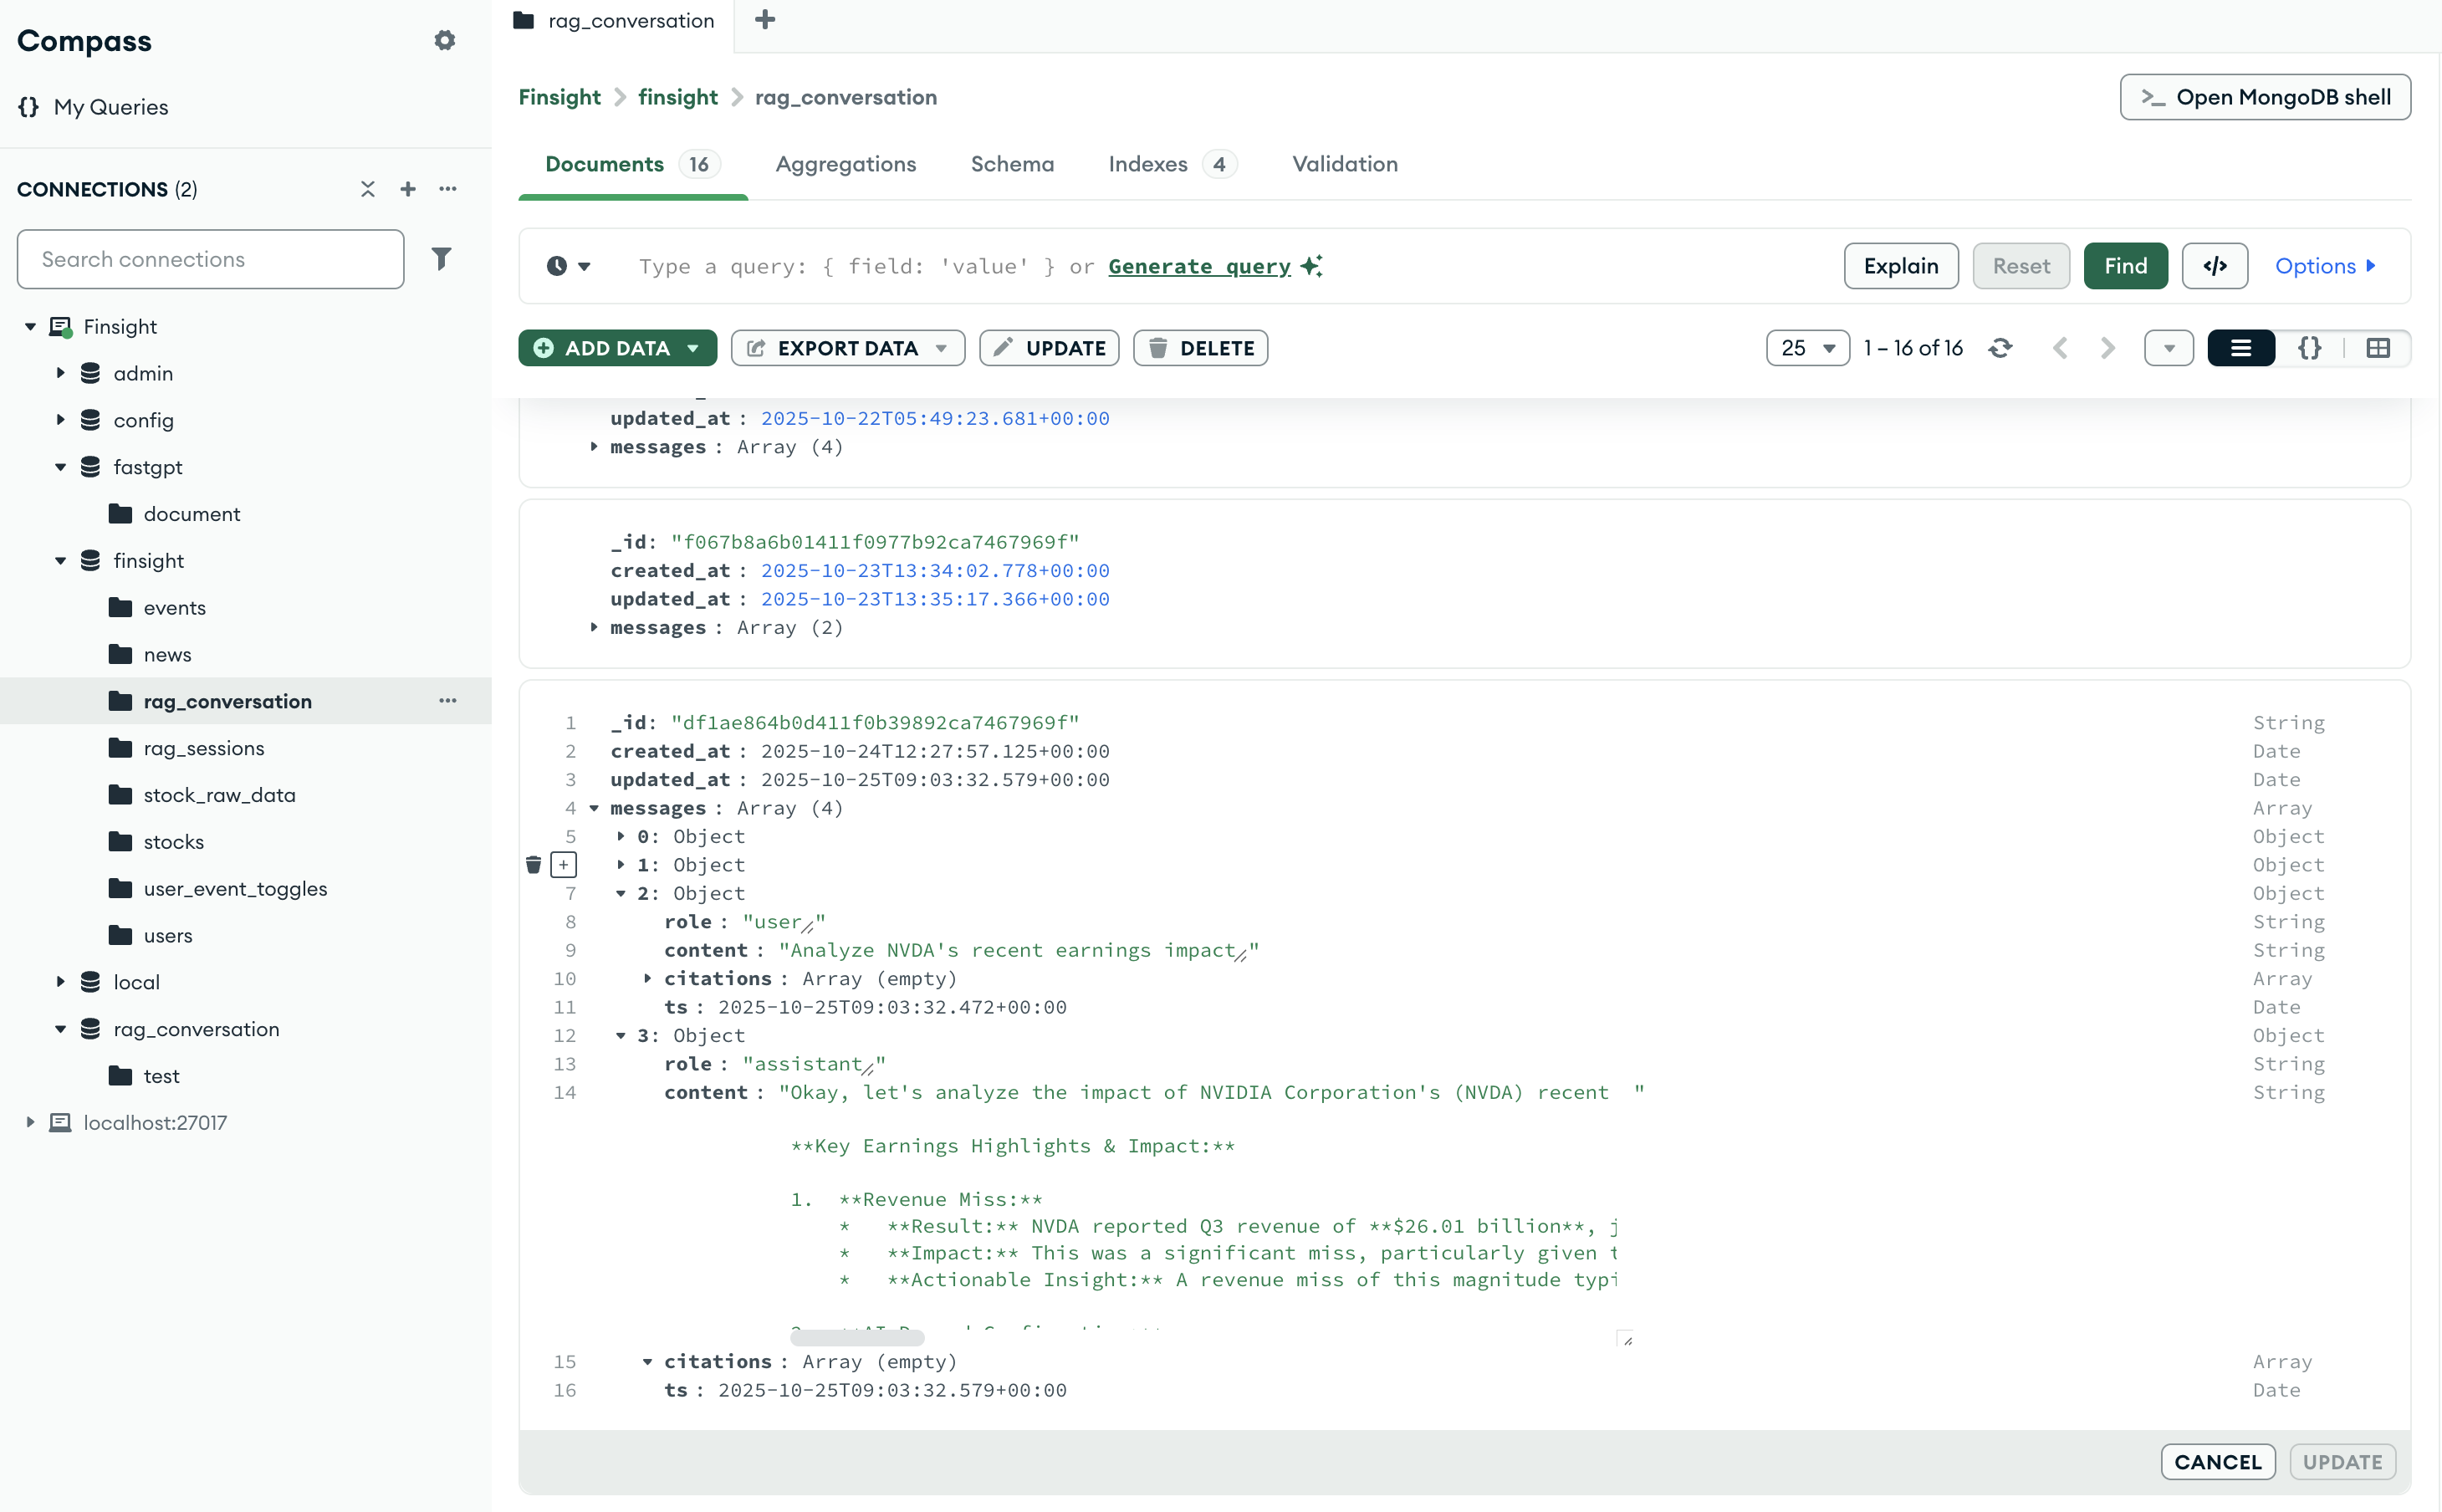
\includegraphics[width=0.75\linewidth]{images/rag_session.png}
    \caption{RAG session and chat history}
\end{center}

\subsection{Prompt Design}
We construct each request with a fixed, evidence-first order to reduce hallucination and keep tone consistent across turns. The system prompt (front-loaded) encodes the grounding policy (summarize from the knowledge base first; disclose fallback reasoning when evidence is thin; keep answers concise and actionable). It is followed by the retrieved knowledge base snippets (de-duplicated and score-truncated), optional recommendation hints (tickers/themes used only as light guidance), and the user query plus minimal session context. This layout ensures KB evidence dominates the model’s attention while recommendations steer specificity without overriding facts; multi-turn continuity is maintained by carrying the session context.

\begin{tcolorbox}
\textbf{System Prompt} \\
\small
\textbf{You are an expert financial research assistant.} Your goal is to provide accurate,
well-reasoned, and context-aware answers using the retrieved knowledge base and your own analytical ability.

\textbf{Instruction:}
1) \textbf{Primary Source:} Prioritize and summarize from the provided knowledge base; cite when relevant. \\
2) \textbf{Fallback Reasoning:} If evidence is insufficient, extend with general financial knowledge and state this explicitly. \\
3) \textbf{Context Awareness:} Respect conversation history and the user’s intent for continuity. \\
4) \textbf{Transparency:} When mainly using general reasoning, begin with a short disclaimer (e.g., “Based on general market understanding…”). \\
5) \textbf{Answer Format:} Be concise and structured; use bullets or short paragraphs; include numbers/dates/ratios and, when appropriate, both \emph{summary} and \emph{implications}.

\medskip
\textbf{Here is the current knowledge base:}

\{knowledge\}

\medskip
When relevant, include market implications or actionable insights (e.g., effects on prices, sectors, or macro indicators).
(If the above is empty or irrelevant, follow the Fallback Reasoning guideline.)
\end{tcolorbox}

Model inputs are concatenated in a fixed order: System Prompt → Knowledge Base Snippet (RAG) → Recommendation Result Prompt (optional, low-weight) → User Question. This design ensures that answers are first summarized based on the retrieved knowledge base, and when insufficient evidence is provided, explicitly triggers the "common market understanding" fallback reasoning, maintaining a consistent tone and context across multiple rounds of dialogue. To reduce hallucinations and redundancy, we deduplicate retrieved snippets, prune them by score, and allocate token budget primarily to knowledge base content. Recommendation prompts retain only symbolic clues to enhance relevance without overriding factual evidence.

\textbf{Conclusion: } The implementation of the AI Analyst subsystem in FinSight successfully integrates retrieval-based factual grounding with generative reasoning to deliver accurate, explainable, and context-aware financial insights. By combining RagFlow’s high-performance retriever and large language model orchestration with FinSight’s modular backend design, the system achieves seamless end-to-end data flow --- from user query submission and document retrieval to structured answer generation and persistent history management. The integration with MongoDB ensures long-term session continuity, while the layered prompt strategy guarantees consistent reasoning behavior and transparency. Overall, the RAG module enhances both the interpretability and reliability of AI-driven financial analysis, enabling users to obtain not only direct answers but also evidence-backed reasoning paths that improve trust and decision confidence.


% \section{Combined Investment Recommendation Module}

% In its initial phase, the module is expected to improve analytic efficiency by reducing the time analysts spend on data collection and cleaning, allowing them to focus more on interpretation. It will produce reports with consistent metrics and transparent assumptions, making peer comparisons easier. Users will be able to respond more quickly to earnings releases, regulatory changes, and macro events, while also gaining better awareness of downside risks through scenario analysis and sensitivity checks. Over time, the system will support benchmarking of its outputs against actual market outcomes, providing a feedback loop on accuracy. For example, for a mid-cap stock, the module should be able to generate valuation estimates reasonably close to market consensus, even within a ±10–20\% range, acknowledging market volatility.



    %\chapter{Challenges}
\section{News Browsing Module}

The challenges anticipated in the proposal proved accurate: rampant content copying impacts ranking; aliasing across tickers and cross-language names can mis-link entities; and it is non-trivial to balance system complexity with both low latency and freshness. 

In practice, we addressed these by:

\begin{enumerate}
	\item aggressive de-duplication and soft penalties for near-duplicates;
	\item  a stricter ticker extraction and post-hoc “seen-ID” filter to avoid showing recently interacted items; 
	\item a two-tier retrieval strategy (cached DB-only by default; tiny live refresh on demand) that keeps the interface responsive even under tight API limits. 
\end{enumerate}


Finally, we use incremental, bounded updates to the 20-d profile so that feedback is responsive without becoming volatile---an answer to the proposal’s concern that profile vectors must adapt frequently without instability.

\section{Stock Recommendation Module}

The development and deployment of the recommendation engine present several anticipated challenges that the project will need to address:

Cold Start Problem: A significant challenge will be providing accurate and engaging recommendations for new users who have no browsing history, making their profile vector non-existent or very sparse. 

Defining and Evaluating 'Success': While offline metrics like Recall@K are valuable, the true measure of success is user engagement and investment decisions, which are more difficult to quantify. How to accurately evaluate the recommendation engine's business impact will be a non-trivial challenge.

Dynamic Nature of Financial Data: User interests and market conditions change rapidly. A user's profile vector must be updated frequently to reflect their evolving preferences. How to determine the optimal update frequency and decay rate for the user profile to remain responsive without becoming overly volatile

\section{Stock Prediction System}


Several challenges encountered during implementation closely aligned with the initial expectations.  
The inherent non-stationarity of financial time series led to unstable performance when market regimes shifted,  
and striking a balance between short-horizon reactivity and longer-horizon consistency proved non-trivial.  
In addition, the need to maintain low-latency forecasting while continuously updating data streams introduced further engineering constraints.   

In practice, we addressed these challenges by:
\begin{enumerate}
    \item implementing an adaptive model-selection mechanism that automatically switches between ARIMA, LSTM, Seq2Seq, and Transformer forecasters based on data length and volatility, reducing overfitting to transient market noise;
    \item applying log-scale normalization and rolling-window retraining to smooth sudden shocks while maintaining sensitivity to trend reversals;
    \item introducing asynchronous data caching and lightweight API responses in FastAPI to minimize delay between inference and visualization.
\end{enumerate}
We perform bounded updates to model states and cached predictions, 
ensuring that forecast outputs remain consistent and responsive without oscillating under volatile market conditions.



\section{AI Analyst}

During the development of the AI Analyst subsystem, several technical challenges were encountered.
\begin{enumerate}
    \item First, integrating RagFlow’s OpenAI-compatible API with the FastAPI backend required careful handling of asynchronous requests and session lifecycle management, as improper timing often caused session conflicts or context loss.
    \item Second, ensuring persistent and consistent chat histories across user sessions posed difficulties in MongoDB schema design and index optimization, especially when dealing with large, nested message structures.
    \item Third, the coordination between document retrieval and generation demanded fine-tuning of the semantic similarity thresholds to balance recall and precision, preventing both information redundancy and retrieval misses.
    \item Fourth, prompt engineering proved challenging, as the system had to maintain consistent model behavior while allowing limited user customization without exposing internal system prompts.
\end{enumerate}

% \section{Combined Investment Recommendation Module}
	\chapter{Conclusion}

\section{Findings and Discussion}
This implementation draws directly on concepts from our Intelligent Reasoning Systems course. By combining knowledge representation, reasoning under uncertainty, and data-driven inference, the system goes beyond raw computation to provide structured, explainable, and evidence-backed financial recommendations. The ability to integrate symbolic reasoning (rules, scenarios, constraints) with statistical methods (LLMs, embeddings, sentiment models) demonstrates how intelligent reasoning frameworks can be applied to real-world domains like financial analysis and investment decision-support.


\section{Future Work}
\subsection{News}

\begin{enumerate}
    \item Broader sources & quality scoring — Add filings / earnings calls / research notes with dedup, entity normalization, and quality scores.
    \item Event extraction — Structure key events (earnings surprise) for downstream use.
\end{enumerate}

\subsection{Recommend}

\begin{enumerate}
    \item Hybrid ranking with finance signals — Fuse content vectors with factor signals (value, quality, momentum), analyst ratings, and sector priors.
    \item Explainability & risk overlays — Show “why recommended” (similar news, factors, peers) and attach risk notes (volatility, drawdown, earnings dates).
\end{enumerate}

\subsection{Forecast}

\begin{enumerate}
    \item Model upgrades — Add TFT/N-BEATS/Informer and consider regime-aware modeling.
    \item Richer features — Macro, events, flows, sentiment/topics to improve signal quality.
\end{enumerate}

\subsection{AI Analyst}

\begin{enumerate}
    \item Grounded answers — Stronger citation/attribution and fallback disclaimers when KB is weak.
    \item Tool calling — Integrate functions (quotes, fundamentals, backtests) via tool/agent calls.
\end{enumerate}
    %\chapter{eg}
\section{Figures}

A test figure is shown in Figure~\ref{fig:test1}.

\begin{figure}[ht!] % supposedly places it here ...
	\centering
	
\includegraphics[width=0.6\linewidth]{test_image_goku}
	\caption[This is the short caption for List of Figures]{A test figure.  This caption is huge, but in the list of figures only the smaller version in the square brackets will appear.\index{Goku il-king}}
	\label{fig:test1}
\end{figure}



\section{Two Side-by-Side Figures}

Two figures shown side-by-side are shown in Figure~\ref{fig:test2}.

\begin{figure}[!ht]
	\centering
	\subbottom[Goku]{
\includegraphics[width=0.3\textwidth]{test_image_goku}}\qquad
	\subbottom[More Goku]{
\includegraphics[width=0.3\textwidth]{test_image_goku}}%
	\caption[Short Caption]{The same super saiyan. Two times.}        
	\label{fig:test2}
\end{figure}


\section{Acronyms}

In the early nineties, \acs{GSM} was deployed in many European countries. \ac{GSM} offered for the first time international roaming for mobile subscribers. The \acs{GSM}’s use of \ac{TDMA} as its communication standard was debated at length. And every now and then there are big discussion whether \ac{CDMA} should have been chosen over \ac{TDMA}.

If you want to know more about \acf{GSM}, \acf{TDMA}, \acf{CDMA} and other acronyms, just read a book about mobile communication. Just to mention it: There is another \ac{UA}, for testing.


\section{Tables}

A beautiful table is shown in Table~\ref{tab:sometable}, data from \textcite{Ebejer2012}.

\begin{table*}\centering
	\ra{1.3}
	\caption{A Beautiful and Complex Table (for tables captions above)}\label{tab:sometable}	
	\begin{tabular}{@{}rrrrcrrr@{}}\toprule
		& \multicolumn{3}{c}{$w = 8$} & \phantom{abc}& \multicolumn{3}{c}{$w = 16$} \\
		\cmidrule{2-4} \cmidrule{6-8} 
		& $t=0$ & $t=1$ & $t=2$ && $t=0$ & $t=1$ & $t=2$\\ \midrule
		$dir=1$\\
		$c$ & 0.0790 & 0.1692 & 0.2945 && 0.3670 & 0.7187 & 3.1815\\
		$c$ & -0.8651& 50.0476& 5.9384&& -9.0714& 297.0923& 46.2143\\
		$c$ & 124.2756& -50.9612& -14.2721&& 128.2265& -630.5455& -381.0930\\
		$dir=0$\\
		$c$ & 0.0357& 1.2473& 0.2119&& 0.3593& -0.2755& 2.1764\\
		$c$ & -17.9048& -37.1111& 8.8591&& -30.7381& -9.5952& -3.0000\\
		$c$ & 105.5518& 232.1160& -94.7351&& 100.2497& 141.2778& -259.7326\\
		\bottomrule
	\end{tabular}
\end{table*}


\section{Long Tables}

The following is an example of a table (Table~\ref{tab:full_dude_results}) spanning multiple pages.

\newcolumntype{P}[1]{>{\centering\arraybackslash}p{#1}}
\begin{center}
	\begingroup
	\renewcommand\arraystretch{0.66} % only applicable to this table because of group
	
	\begin{longtable}{lrrrrrrrr}
		\caption[Performance of Ligity in HTS mode against the Ligity-compatible DUD-E targets]{Performance of Ligity in HTS mode against the Ligity-compatible DUD-E targets. The mean (and standard deviation in parentheses) values of ROC AUC using Tanimoto is 0.622 ($\pm 0.132$), while for Tversky it is 0.671 ($\pm 0.142$); the mean EF\textsubscript{1\%} using Tanimoto is 5.648 ($\pm 8.668$), while for EF\textsubscript{1\%} using Tversky it is 9.047 ($\pm 12.713$).} 
		\label{tab:full_dude_results} 
		\\ 
		\toprule 
		\multicolumn{1}{l}{\textbf{Target}}
		& \multicolumn{1}{P{1cm}}{\textbf{No.\ of Actives}}
		& \multicolumn{1}{P{1cm}}{\textbf{No.\ of Decoys}} 
		& \multicolumn{1}{P{1.25cm}}{\textbf{ROC AUC Tanimoto}} 
		& \multicolumn{1}{P{1.25cm}}{\textbf{ROC AUC Tversky}} 
		& \multicolumn{1}{P{1.25cm}}{\textbf{BEDROC Tanimoto}} 
		& \multicolumn{1}{P{1.25cm}}{\textbf{BEDROC Tversky}} 
		& \multicolumn{1}{P{1.25cm}}{\textbf{EF\textsubscript{1\%} Tanimoto}} 
		& \multicolumn{1}{P{1.5cm}}{\textbf{EF\textsubscript{1\%} Tversky}}\\	
		\midrule
		\endfirsthead
		\midrule
		\multicolumn{1}{l}{\textbf{Target}}
		& \multicolumn{1}{P{1cm}}{\textbf{No.\ of Actives}}
		& \multicolumn{1}{P{1cm}}{\textbf{No.\ of Decoys}} 
		& \multicolumn{1}{P{1.25cm}}{\textbf{ROC AUC Tanimoto}} 
		& \multicolumn{1}{P{1.25cm}}{\textbf{ROC AUC Tversky}}
		& \multicolumn{1}{P{1.25cm}}{\textbf{BEDROC Tanimoto}} 
		& \multicolumn{1}{P{1.25cm}}{\textbf{BEDROC Tversky}} 
		& \multicolumn{1}{P{1.25cm}}{\textbf{EF\textsubscript{1\%} Tanimoto}} 
		& \multicolumn{1}{P{1.25cm}}{\textbf{EF\textsubscript{1\%} Tversky}}\\	
		\midrule	
		\endhead
		\midrule	
		\multicolumn{7}{r@{}}{(continued\ldots)}\\
		\endfoot
		\endlastfoot
		ABL1   & 182   & 10,750   & 0.563   & 0.473   & 0.077   & 0.077   & 1.653   & 2.204  \\
		ACE    & 281   & 16,877   & 0.787   & 0.787   & 0.336   & 0.401   & 12.425  & 19.525 \\
		ACES   & 453   & 26,242   & 0.634   & 0.645   & 0.077   & 0.155   & 1.766   & 5.518  \\
		ADA    & 93    & 5,450    & 0.724   & 0.660   & 0.149   & 0.147   & 3.251   & 3.251  \\
		ADA17  & 532   & 35,898   & 0.638   & 0.728   & 0.103   & 0.283   & 1.317   & 9.030  \\
		ADRB1  & 247   & 15,850   & 0.523   & 0.647   & 0.065   & 0.129   & 1.619   & 5.262  \\
		ADRB2  & 231   & 14,999   & 0.523   & 0.589   & 0.052   & 0.040   & 1.735   & 0.000  \\
		AKT1   & 293   & 16,450   & 0.386   & 0.548   & 0.039   & 0.107   & 2.737   & 3.080  \\
		AKT2   & 117   & 6,900    & 0.511   & 0.685   & 0.140   & 0.194   & 8.568   & 8.568  \\
		ALDR   & 159   & 8,988    & 0.574   & 0.610   & 0.202   & 0.172   & 10.747  & 6.322  \\
		AMPC   & 48    & 2,845    & 0.521   & 0.541   & 0.049   & 0.023   & 0.000   & 0.000  \\
		ANDR   & 269   & 14,349   & 0.722   & 0.742   & 0.194   & 0.354   & 4.839   & 24.938 \\
		AOFB   & 121   & 6,875    & 0.422   & 0.464   & 0.045   & 0.027   & 1.652   & 0.000  \\
		BACE1  & 283   & 18,100   & 0.441   & 0.775   & 0.017   & 0.310   & 0.000   & 13.062 \\
		BRAF   & 152   & 9,950    & 0.612   & 0.639   & 0.208   & 0.165   & 12.502  & 5.264  \\
		CASP3  & 199   & 10,694   & 0.600   & 0.734   & 0.068   & 0.258   & 0.502   & 7.031  \\
		CDK2   & 474   & 27,838   & 0.467   & 0.507   & 0.021   & 0.048   & 0.000   & 1.055  \\
		COMT   & 41    & 3,846    & 0.789   & 0.889   & 0.338   & 0.665   & 19.447  & 58.341 \\
		CP2C9  & 120   & 7,449    & 0.518   & 0.634   & 0.058   & 0.186   & 1.660   & 8.299  \\
		CP3A4  & 170   & 11,787   & 0.450   & 0.493   & 0.022   & 0.057   & 0.000   & 2.345  \\
		CSF1R  & 166   & 12,149   & 0.526   & 0.542   & 0.136   & 0.152   & 6.031   & 7.238  \\
		CXCR4  & 40    & 3,405    & 0.575   & 0.722   & 0.217   & 0.134   & 12.665  & 0.000  \\
		DEF    & 102   & 5,699    & 0.732   & 0.833   & 0.212   & 0.379   & 10.786  & 15.689 \\
		DHI1   & 330   & 19,348   & 0.481   & 0.595   & 0.089   & 0.062   & 2.422   & 1.211  \\
		DPP4   & 533   & 40,941   & 0.586   & 0.591   & 0.154   & 0.157   & 4.312   & 3.937  \\
		DRD3   & 480   & 34,048   & 0.484   & 0.441   & 0.043   & 0.046   & 1.251   & 0.626  \\
		DYR    & 231   & 17,196   & 0.694   & 0.758   & 0.210   & 0.230   & 6.504   & 7.371  \\
		EGFR   & 542   & 35,047   & 0.593   & 0.491   & 0.054   & 0.037   & 0.922   & 0.000  \\
		ESR1   & 383   & 20,683   & 0.838   & 0.861   & 0.527   & 0.594   & 31.281  & 39.101 \\
		ESR2   & 367   & 20,199   & 0.844   & 0.870   & 0.563   & 0.644   & 20.130  & 32.644 \\
		FA10   & 537   & 28,324   & 0.564   & 0.674   & 0.058   & 0.118   & 0.930   & 2.232  \\
		FA7    & 114   & 6,249    & 0.762   & 0.859   & 0.210   & 0.332   & 6.105   & 8.721  \\
		FABP4  & 47    & 2,749    & 0.786   & 0.744   & 0.191   & 0.276   & 0.000   & 10.623 \\
		FAK1   & 100   & 5,350    & 0.642   & 0.531   & 0.111   & 0.065   & 2.019   & 0.000  \\
		FGFR1  & 139   & 8,698    & 0.511   & 0.522   & 0.036   & 0.088   & 0.722   & 1.445  \\
		FKB1A  & 111   & 5,799    & 0.605   & 0.751   & 0.162   & 0.164   & 8.122   & 3.610  \\
		FNTA   & 592   & 51,493   & 0.411   & 0.625   & 0.012   & 0.132   & 0.000   & 4.053  \\
		FPPS   & 85    & 8,842    & 0.917   & 0.985   & 0.323   & 0.776   & 2.360   & 36.581 \\
		GCR    & 258   & 14,998   & 0.805   & 0.834   & 0.244   & 0.324   & 3.092   & 8.116  \\
		GLCM   & 54    & 3,790    & 0.667   & 0.685   & 0.182   & 0.279   & 1.873   & 11.240 \\
		GRIA2  & 158   & 11,842   & 0.662   & 0.684   & 0.248   & 0.154   & 11.392  & 5.696  \\
		GRIK1  & 101   & 6,547    & 0.656   & 0.668   & 0.203   & 0.102   & 7.978   & 1.995  \\
		HDAC2  & 185   & 10,300   & 0.676   & 0.734   & 0.187   & 0.201   & 4.318   & 4.318  \\
		HDAC8  & 170   & 10,449   & 0.640   & 0.819   & 0.120   & 0.377   & 2.946   & 8.250  \\
		HIVINT & 100   & 6,640    & 0.390   & 0.554   & 0.030   & 0.116   & 0.000   & 3.018  \\
		HIVPR  & 535   & 35,724   & 0.663   & 0.872   & 0.072   & 0.490   & 0.187   & 23.898 \\
		HIVRT  & 338   & 18,884   & 0.495   & 0.475   & 0.124   & 0.085   & 4.443   & 1.777  \\
		HMDH   & 170   & 8,750    & 0.480   & 0.906   & 0.068   & 0.652   & 2.358   & 35.963 \\
		HS90A  & 88    & 4,850    & 0.635   & 0.506   & 0.096   & 0.083   & 0.000   & 3.436  \\
		HXK4   & 92    & 4,700    & 0.662   & 0.803   & 0.206   & 0.307   & 15.192  & 9.766  \\
		IGF1R  & 148   & 9,300    & 0.502   & 0.575   & 0.057   & 0.189   & 2.037   & 14.941 \\
		INHA   & 43    & 2,300    & 0.493   & 0.575   & 0.031   & 0.045   & 0.000   & 0.000  \\
		ITAL   & 138   & 8,500    & 0.619   & 0.465   & 0.037   & 0.065   & 0.000   & 0.728  \\
		JAK2   & 107   & 6,500    & 0.472   & 0.475   & 0.073   & 0.118   & 2.807   & 6.549  \\
		KIF11  & 116   & 6,850    & 0.755   & 0.781   & 0.149   & 0.219   & 4.289   & 2.574  \\
		KIT    & 166   & 10,449   & 0.463   & 0.437   & 0.045   & 0.030   & 0.000   & 0.000  \\
		KITH   & 57    & 2,850    & 0.649   & 0.838   & 0.228   & 0.709   & 14.069  & 47.483 \\
		KPCB   & 135   & 8,699    & 0.753   & 0.813   & 0.220   & 0.338   & 8.923   & 12.641 \\
		LCK    & 419   & 27,391   & 0.471   & 0.437   & 0.031   & 0.043   & 0.000   & 1.910  \\
		LKHA4  & 171   & 9,448    & 0.718   & 0.694   & 0.238   & 0.150   & 8.203   & 1.758  \\
		MAPK2  & 101   & 6,148    & 0.660   & 0.670   & 0.174   & 0.199   & 5.988   & 3.992  \\
		MCR    & 94    & 5,149    & 0.816   & 0.888   & 0.215   & 0.454   & 6.436   & 19.307 \\
		MET    & 166   & 11,249   & 0.566   & 0.531   & 0.130   & 0.065   & 6.032   & 0.603  \\
		MK01   & 79    & 4,550    & 0.518   & 0.602   & 0.121   & 0.206   & 5.095   & 3.821  \\
		MK10   & 104   & 6,600    & 0.488   & 0.489   & 0.020   & 0.031   & 0.962   & 0.962  \\
		MK14   & 578   & 35,847   & 0.511   & 0.589   & 0.040   & 0.064   & 0.173   & 0.519  \\
		MMP13  & 572   & 37,199   & 0.648   & 0.753   & 0.134   & 0.268   & 2.446   & 9.957  \\
		MP2K1  & 121   & 8,146    & 0.669   & 0.569   & 0.187   & 0.058   & 3.293   & 0.823  \\
		NOS1   & 98    & 8,028    & 0.483   & 0.451   & 0.109   & 0.041   & 3.071   & 0.000  \\
		NRAM   & 98    & 6,200    & 0.853   & 0.859   & 0.342   & 0.290   & 11.221  & 3.060  \\
		PA2GA  & 99    & 5,150    & 0.793   & 0.756   & 0.225   & 0.153   & 1.020   & 3.059  \\
		PARP1  & 508   & 30,029   & 0.635   & 0.692   & 0.215   & 0.231   & 11.234  & 7.884  \\
		PGH1   & 195   & 10,798   & 0.645   & 0.637   & 0.077   & 0.100   & 0.000   & 2.050  \\
		PGH2   & 435   & 23,139   & 0.716   & 0.780   & 0.166   & 0.291   & 3.444   & 9.874  \\
		PLK1   & 107   & 6,800    & 0.658   & 0.531   & 0.123   & 0.048   & 1.871   & 0.000  \\
		PNPH   & 103   & 6,946    & 0.575   & 0.578   & 0.161   & 0.181   & 4.888   & 8.799  \\
		PPARA  & 373   & 19,399   & 0.783   & 0.778   & 0.262   & 0.280   & 6.693   & 7.764  \\
		PPARD  & 240   & 12,250   & 0.547   & 0.544   & 0.078   & 0.098   & 1.665   & 2.498  \\
		PPARG  & 484   & 25,299   & 0.515   & 0.605   & 0.055   & 0.118   & 0.619   & 4.955  \\
		PRGR   & 293   & 15,648   & 0.740   & 0.793   & 0.142   & 0.318   & 2.053   & 14.714 \\
		PTN1   & 130   & 7,249    & 0.398   & 0.538   & 0.055   & 0.090   & 0.000   & 3.068  \\
		PUR2   & 50    & 2,700    & 0.851   & 0.837   & 0.281   & 0.255   & 7.857   & 1.964  \\
		PYGM   & 77    & 3,944    & 0.403   & 0.492   & 0.016   & 0.137   & 0.000   & 3.917  \\
		PYRD   & 111   & 6,449    & 0.682   & 0.710   & 0.462   & 0.413   & 34.027  & 16.118 \\
		RENI   & 104   & 6,956    & 0.720   & 0.789   & 0.043   & 0.138   & 0.000   & 0.000  \\
		ROCK1  & 100   & 6,300    & 0.347   & 0.449   & 0.020   & 0.084   & 1.000   & 4.000  \\
		RXRA   & 131   & 6,950    & 0.788   & 0.900   & 0.219   & 0.596   & 6.091   & 27.407 \\
		SAHH   & 63    & 3,450    & 0.874   & 0.852   & 0.598   & 0.542   & 35.050  & 27.084 \\
		SRC    & 524   & 34,500   & 0.565   & 0.477   & 0.065   & 0.050   & 0.382   & 0.573  \\
		TGFR1  & 133   & 8,499    & 0.609   & 0.639   & 0.147   & 0.154   & 10.565  & 4.528  \\
		THB    & 103   & 7,450    & 0.794   & 0.762   & 0.238   & 0.150   & 10.614  & 0.965  \\
		THRB   & 461   & 27,000   & 0.605   & 0.706   & 0.063   & 0.166   & 2.166   & 5.632  \\
		TRY1   & 449   & 25,975   & 0.711   & 0.815   & 0.147   & 0.280   & 2.898   & 6.688  \\
		TRYB1  & 148   & 7,650    & 0.670   & 0.670   & 0.153   & 0.132   & 3.378   & 3.378  \\
		TYSY   & 109   & 6,745    & 0.594   & 0.725   & 0.071   & 0.226   & 0.911   & 5.468  \\
		UROK   & 162   & 9,850    & 0.525   & 0.650   & 0.036   & 0.120   & 0.000   & 1.854  \\
		VGFR2  & 409   & 24,948   & 0.632   & 0.578   & 0.083   & 0.093   & 1.465   & 1.465  \\
		WEE1   & 102   & 6,150    & 0.934   & 0.929   & 0.789   & 0.797   & 59.348  & 61.294 \\
		XIAP   & 100   & 5,150    & 0.752   & 0.974   & 0.190   & 0.897   & 8.077   & 51.490 \\
		\bottomrule
	\end{longtable}
	
	\endgroup
\end{center}



\section{Landscape Tables}
Next is an example of a wide table on a landscape oriented paper (Table~\ref{tab:land}).

\begin{landscape}
	\pagestyle{empty} %% only if you want to remove silly headers on the side	
	\begin{table}[h]
		\caption[A landscape table]{A table in landscape orientation.} 
		\begin{tabular}{rrrrrrrrrrrrrrr} \toprule
			\label{tab:land} 		
			{$m$} & {$x$} & {$y$} & {$z$} & {$a$} & {$A_m$} & {$B$} & {$C$} & {$x$} & {$y$} & {$z$} & {$a$} & {$A_m$} & {$B$} & {$C$} \\ \midrule
			1  & 16.128 & +8.872 & 16.128 & 1.402 & 1.373 & -146.6 & -137.6 & 16.128 & +8.872 & 16.128 & 1.402 & 1.373 & -146.6 & -137.6\\
			2  & 3.442  & -2.509 & 3.442  & 0.299 & 0.343 & 133.2  & 152.4 & 3.442  & -2.509 & 3.442  & 0.299 & 0.343 & 133.2  & 152.4 \\
			3  & 1.826  & -0.363 & 1.826  & 0.159 & 0.119 & 168.5  & -161.1 & 1.826  & -0.363 & 1.826  & 0.159 & 0.119 & 168.5  & -161.1 \\
			4  & 0.993  & -0.429 & 0.993  & 0.086 & 0.08  & 25.6   & 90 & 1.826  & -0.363 & 1.826  & 0.159 & 0.119 & 168.5  & -161.1    \\ \midrule
			5  & 1.29   & +0.099 & 1.29   & 0.112 & 0.097 & -175.6 & -114.7 & 1.826  & -0.363 & 1.826  & 0.159 & 0.119 & 168.5  & -161.1\\
			6  & 0.483  & -0.183 & 0.483  & 0.042 & 0.063 & 22.3   & 122.5 & 1.826  & -0.363 & 1.826  & 0.159 & 0.119 & 168.5  & -161.1 \\
			7  & 0.766  & -0.475 & 0.766  & 0.067 & 0.039 & 141.6  & -122 & 1.826  & -0.363 & 1.826  & 0.159 & 0.119 & 168.5  & -161.1  \\
			8  & 0.624  & +0.365 & 0.624  & 0.054 & 0.04  & -35.7  & 90  & 1.826  & -0.363 & 1.826  & 0.159 & 0.119 & 168.5  & -161.1   \\ \midrule
			9  & 0.641  & -0.466 & 0.641  & 0.056 & 0.045 & 133.3  & -106.3 & 1.826  & -0.363 & 1.826  & 0.159 & 0.119 & 168.5  & -161.1\\
			10 & 0.45   & +0.421 & 0.45   & 0.039 & 0.034 & -69.4  & 110.9  & 1.826  & -0.363 & 1.826  & 0.159 & 0.119 & 168.5  & -161.1\\
			11 & 0.598  & -0.597 & 0.598  & 0.052 & 0.025 & 92.3   & -109.3 & 1.826  & -0.363 & 1.826  & 0.159 & 0.119 & 168.5  & -161.1\\ \bottomrule
		\end{tabular}
	\end{table}
\end{landscape}


\section{Theorems}

\begin{theorem}
	Let \(f\) be a function whose derivative exists in every point, then \(f\) is 
	a continuous function.
\end{theorem}

\begin{theorem}[Pythagorean theorem]
	\label{pythagorean}
	This is a theorem about right triangles and can be summarised in the next 
	equation 
	\[ x^2 + y^2 = z^2 \]
\end{theorem}

And a consequence of Theorem \ref{pythagorean} is the statement in the next corollary.

\begin{corollary}
	There's no right rectangle whose sides measure 3~cm, 4~cm, and 6~cm.
\end{corollary}

You can reference theorems such as \ref{pythagorean} when a label is assigned.


\section{Lemmas}

\begin{lemma}
	Given two line segments whose lengths are \(a\) and \(b\) respectively there is a 
	real number \(r\) such that \(b=ra\).
\end{lemma}


\section{Proofs}

\begin{lemma}
	Given two line segments whose lengths are \(a\) and \(b\) respectively there 
	is a real number \(r\) such that \(b=ra\).
\end{lemma}

\begin{proof}
	To prove it by contradiction try and assume that the statement is false,
	proceed from there and at some point you will arrive to a contradiction.
\end{proof}


\section{Code Listings}

Here you go.

\begin{lstlisting}[language=Python,caption={My Listing Caption},captionpos=b]
	import numpy as np
	
	def incmatrix(genl1,genl2):
	m = len(genl1)
	n = len(genl2)
	M = None #to become the incidence matrix
	VT = np.zeros((n*m,1), int)  #dummy variable
	
	#compute the bitwise xor matrix
	M1 = bitxormatrix(genl1)
	M2 = np.triu(bitxormatrix(genl2),1) 
	
	for i in range(m-1):
	for j in range(i+1, m):
	[r,c] = np.where(M2 == M1[i,j])
	for k in range(len(r)):
	VT[(i)*n + r[k]] = 1;
	VT[(i)*n + c[k]] = 1;
	VT[(j)*n + r[k]] = 1;
	VT[(j)*n + c[k]] = 1;
	
	if M is None:
	M = np.copy(VT)
	else:
	M = np.concatenate((M, VT), 1)
	
	VT = np.zeros((n*m,1), int)
	
	return M
\end{lstlisting}



\section{Algorithms}


%% This is needed if you want to add comments in
%% your algorithm with \Comment
\SetKwComment{Comment}{/* }{ */}

\begin{algorithm}[hbt!]
	\caption{An algorithm with caption}\label{alg:example}
	\KwData{$n \geq 0$}
	\KwResult{$y = x^n$}
	$y \gets 1$\;
	$X \gets x$\;
	$N \gets n$\;
	\While{$N \neq 0$}{
		\eIf{$N$ is even}{
			$X \gets X \times X$\;
			$N \gets \frac{N}{2} $ \Comment*[r]{This is a comment}
		}{\If{$N$ is odd}{
				$y \gets y \times X$\;
				$N \gets N - 1$\;
			}
		}
	}
\end{algorithm}

An algorithm example is shown in Algorithm~\ref{alg:example}. \blindtext

\section{Suppressing Page Numbers on a Float Page}

Kindly refer to Figure~\ref{fig:largegoku}. 



\begin{figure}[!ht]
	\thisfloatpagestyle{empty} %% This is the key line to suppress page decorations (including nos.) on float pages.
	\centering
	
\includegraphics[width=0.9\textwidth]{goku-large}
	\caption[Short Random Caption]{Page numbers are suppressed on this page.}
	\label{fig:largegoku}
\end{figure}


\FloatBarrier % from placeins

\section{Referencing}

Use \texttt{\textbackslash textcite} for in-text citations, e.g.\ \textcite{Einstein1905}, and \texttt{\textbackslash parencite} for citations in parenthesis. And this is what an online reference looks like \parencite{WinNT}.

In their study, \textcite{Einstein1905} show the world is round. Others have shown this to be the case \parencite{Arrighi2003, Ebejer2016}.

\section{Using a Different Language}

\begin{otherlanguage}{maltese}
Local name $=$ Malti. Today $=$ \today. Jiena ngħix Ħaż-Żebbuġ.
\end{otherlanguage}

\section{Summary}



\appendix
	\chapter{Project Proposal}
\includepdf[pages=-]{appA/Group_6_proposal_final.pdf}     % these are just test names as I didn't know what you'd want
	\chapter{Mapped System Functionalities}
\thispagestyle{plain}  % optional: 保留页码
\vspace*{-1cm}         % 向上收紧空间,调整为适合位置
\noindent 

\begin{table}[H]
\centering
\caption{Mapping of System Functionalities against Knowledge, Techniques, and Skills from MR, RS, and CGS Courses}
\renewcommand{\arraystretch}{1.3}
\begin{tabular}{|p{2.8cm}|p{5cm}|p{7cm}|}
\hline
\textbf{Course Module} & \textbf{Techniques Covered} & \textbf{Mapped FinSight Functionalities} \\
\hline
\textbf{MR} &
\begin{itemize}
  \item Knowledge representation and reasoning for problem solving
  \item Search and constraint satisfaction reasoning
  \item Machine reasoning over knowledge graphs
  \item Neural and inductive reasoning models
\end{itemize}
&
\begin{itemize}
  \item Knowledge-based stock analysis within the AI Analyst (RAG Assistant) module
  \item Reasoning engine for contextual understanding of user queries
  \item Use of inductive reasoning for suggesting stock recommend explanations
\end{itemize}
\\
\hline
\textbf{RS} &
\begin{itemize}
  \item Market-based and similarity-based recommender systems
  \item Model-based hybrid recommendation design
  \item Knowledge discovery from large datasets
\end{itemize}
&
\begin{itemize}
  \item Stock Recommendation module using similarity and hybrid recommender approaches
  \item User profiling and vector-based preference optimization (content-based + collaborative signals)
  \item News browsing feedback loop employing incremental optimization of user preference vectors
  \item Data-driven reasoning for refining recommendations from large-scale market data
\end{itemize}
\\
\hline
\textbf{CGS} &
\begin{itemize}
  \item Natural language cognition and LLM reasoning
  \item Knowledge representation and reasoning in cognitive systems
  \item Human–AI interaction and chatbot-based communication
\end{itemize}
&
\begin{itemize}
  \item RAG-based AI Financial Analyst for conversational reasoning and decision support
  \item Cognitive interface enabling natural-language interaction between user and system
  \item Contextual retrieval and reasoning using LLMs for personalized financial insights
  \item Knowledge-based dialogue that integrates user intent with domain reasoning
\end{itemize}
\\
\hline
\end{tabular}
\end{table}

\begin{enumerate}
    \item News Module -> Knowledge discovery
	\item Recommendation Module -> Hybrid recommender optimization \ Knowledge discovery
	\item Forecast Module -> Business resource optimization (evolutionary computing)
	\item AI Analyst Module -> Decision automation (knowledge-based reasoning) and Cognitive system design (knowledge graph \& natural-language interface)
\end{enumerate}
    
	\chapter{Installation and User Guide}

\section{Installation}

\subsection{Backend}

\subsubsection{Overview}

\textbf{FinSight} is an AI-powered financial analytics backend that provides news aggregation, vector-based retrieval, stock forecasting, recommendation, and RAG-based financial research assistance — all implemented within a modular \texttt{FastAPI} architecture.

This repository hosts the backend micro-services, which include:

\begin{itemize}
    \item \textbf{News Fetching \& Aggregation}
    \item \textbf{Stock Trend Forecasting} (ARIMA / Prophet / LSTM / LightGBM / Transformer / Seq2Seq)
    \item \textbf{RAG-based Financial Research Analyst}
    \item \textbf{Content-based \& Vector-based Stock Recommendation}
    \item \textbf{User Profiles, Watchlists, and Authentication}
    \item \textbf{MongoDB + Postgres (pgvector) Support}
\end{itemize}

\subsubsection{Project Structure}

\begin{lstlisting}[language={}, basicstyle=\ttfamily\small]
FinSight_BackEnd
├── app
│   ├── adapters
│   │   ├── db
│   │   │   ├── database_client.py
│   │   │   ├── news_repo.py
│   │   │   ├── pg_profile_repo.py
│   │   │   ├── rag_conversation_repo.py
│   │   │   └── user_repo.py
│   │   ├── embeddings
│   │   ├── fetchers
│   │   ├── llm
│   │   ├── rag
│   │   └── vector
│   ├── api
│   │   └── v1
│   │       ├── auth_router.py
│   │       ├── forecast_router.py
│   │       ├── news_router.py
│   │       ├── rag_router.py
│   │       ├── rec_router.py
│   │       ├── stocks_router.py
│   │       └── user_router.py
│   ├── forecasters
│   │   ├── arima_forecaster.py
│   │   ├── prophet_forecaster.py
│   │   ├── lstm_forecaster.py
│   │   ├── transformer_forecaster.py
│   │   └── stacked_forecaster.py
│   ├── services
│   │   ├── news_service.py
│   │   ├── forecast_service.py
│   │   ├── rag_service.py
│   │   ├── rec_service.py
│   │   └── user_service.py
│   └── main.py
├── docker-compose.yml
├── environment.yml
├── finsight_keypair.pem
├── pyproject.toml
├── README.md
└── requirements.txt
\end{lstlisting}

All dependencies are fully managed through \textbf{\texttt{pyproject.toml}}.

\subsubsection{Prerequisites}

\begin{table}[H]
\centering
\caption{System Prerequisites}
\begin{tabular}{|l|l|}
\hline
\textbf{Tool} & \textbf{Requirement} \\
\hline
Python & 3.10+ \\
Docker & Required for Knowledge Base (MongoDB + Postgres) \\
uv / pip & For dependency installation \\
Ragflow & For RAG deployment \\
Ollama & For local LLM provider \\
\hline
\end{tabular}
\end{table}

Installation of \texttt{uv}
\begin{lstlisting}[language=bash]
curl -LsSf https://astral.sh/uv/install.sh | sh
\end{lstlisting}

Database Access (via EC2 Server)

The EC2 server hosts both MongoDB and PostgreSQL databases:

\begin{itemize}
    \item \textbf{MongoDB:} Stores news and optionally vector embeddings.
    \item \textbf{PostgreSQL + pgvector:} Stores user profiles, embeddings, and recommendations.
\end{itemize}

To connect, simply place \texttt{finsight\_keypair.pem} in the project root.  
The program will automatically establish the SSH tunnel and access the databases.

\subsubsection{Optional: RAG Component Deployment}

Due to limited memory on the EC2 server, the RAG module is deployed locally.  
This step is optional and does not affect other backend functionalities.

\begin{enumerate}
    \item \textbf{Deploy Ragflow locally:} Follow the official guide at \texttt{https://ragflow.io/docs/dev/build\_docker\_image}.
    \item \textbf{Run local LLM via Ollama:}
    \begin{lstlisting}[language=bash]
    ollama run deepseek-r1:8b
    \end{lstlisting}
    \item \textbf{Replace your Ragflow key:}  
    Add it to the \texttt{.env} file as:
    \begin{lstlisting}
    RAGFLOW_API_KEY=<your-key>
    \end{lstlisting}
\end{enumerate}

\subsubsection{Installation}

\begin{lstlisting}[language=bash]
git clone https://github.com/jiajun-lab/FinSight_BackEnd.git FinSight_BackEnd
cd FinSight_BackEnd

# Create virtual environment
uv venv
source .venv/bin/activate

# Install dependencies
uv pip install -e .
# (or pip install -e .)
\end{lstlisting}

\textbf{Note:} Prophet will compile CmdStan on first run, which may take several minutes.

\subsubsection{Running the Backend}

Before starting, configure your \texttt{.env} file accordingly.

\begin{lstlisting}[language=bash]
uvicorn app.main:app --reload --port 8000
\end{lstlisting}

API documentation is available at:

\begin{lstlisting}
http://localhost:8000/docs
\end{lstlisting}

The backend service runs on \texttt{http://localhost:8000}, and the frontend retrieves all data from this endpoint.

---

\subsection{Frontend}
\subsubsection{Installation}

\begin{lstlisting}[language=bash]
# 1) Clone this repository
git clone https://github.com/jiajun-lab/FinSight_Frontend.git FinSight_FrontEnd
cd FinSight_FrontEnd

# 2) In this folder:
pnpm i

# 3) set backend endpoint (optional; default already localhost):
echo 'VITE_BACKEND_BASE_URL=http://127.0.0.1:8000' > .env

# 4) run
pnpm dev

# 5) quick restart
rm -rf node_modules pnpm-lock.yaml package-lock.json # optional clean reboot
pnpm i 
pnpm dev 
\end{lstlisting}



\section{News Browsing}

\subsection{Overview}

The FinSight News Browsing Module allows users to explore personalized financial news in an intuitive and interactive interface.  
The system learns from your actions --- such as reading, liking, and bookmarking --- to continuously refine future recommendations.  
This guide explains how to navigate, interact, and get the best experience from the news platform.

\subsection{Getting Started}

\begin{enumerate}
  \item Open the FinSight web application in your browser.
  \item Log in with your registered account.  
  \item Click on the \textbf{“News”} tab in the top navigation bar to enter the news recommendation page.
\end{enumerate}

Once you enter, the system automatically loads your personalized news feed, showing 9 recommended articles in a clean \(3\times3\) grid layout.

\subsection{Browsing the News Feed}

\begin{itemize}
  \item Each news card displays the \textbf{title}, \textbf{source}, \textbf{publication time}, and \textbf{related stock or sector}.
  \item Click the article title to open the full story in a new browser tab.
  \item Use the \textbf{Next} and \textbf{Previous} buttons at the bottom to move between pages.
  \item The system automatically caches previous pages, so navigation is fast and seamless.
  \item When you reach the last page and click \textbf{Next}, new articles will be fetched and displayed automatically.
\end{itemize}

\subsection{Interacting with Articles}

You can directly interact with each article to help the system learn your preferences:

\begin{itemize}
  \item \textbf{Like} (\(\heartsuit\)) — Press this button if you find an article relevant or interesting.  
        Future recommendations will prioritize similar topics or sectors.
  \item \textbf{Bookmark} (\(\star\)) — Use this to save an article for later reading.  
        It also signals a stronger preference to the system.
  \item \textbf{Read} — Simply clicking and reading an article contributes to your profile based on reading duration.
\end{itemize}

All actions update your profile automatically in the background --- there is no need to refresh the page.

\subsection{Getting Personalized Recommendations}

The news feed automatically adapts based on your reading and interaction history:
\begin{itemize}
  \item The more you interact, the more accurate your recommendations become.
  \item You will start seeing more articles from sectors and companies that match your interests.
  \item Older or irrelevant content will gradually fade out as new interests emerge.
\end{itemize}

You can always reset your browsing session by reloading the page --- the system will load a fresh selection of recommended articles.

\subsection{Tips for Best Experience}

\begin{itemize}
  \item Interact regularly (like or bookmark) to personalize your feed faster.
  \item Use \textbf{Next} to load new articles when you reach the end of your feed.
  \item The system automatically avoids showing repeated or recently viewed items.
  \item All updates happen instantly without page reloads.
\end{itemize}


\section{Stock Recommendation}

The Stock Recommendation System helps investors discover suitable investment opportunities through intelligent algorithms and comprehensive stock analysis tools. This manual explains how to use the six main features of the system.

\subsection{Browsing All Stocks}
To explore the complete stock universe:

\begin{enumerate}
    \item Click the \textbf{"All Stocks"} tab in the main navigation.
    \item Use the search bar at the top to find stocks by symbol or company name.
    \item Scroll through the grid layout to view all available stocks.
    \item Each stock card displays:
    \begin{itemize}
        \item Stock symbol and company name
        \item Sector with color coding
        \item Basic financial metrics when available
    \end{itemize}
    \item Click the pagination controls at the bottom to navigate through multiple pages.
    \item Hover over any stock card to trigger pre-loading of detailed information.
\end{enumerate}

\subsection{Getting Basic Recommendations}
To receive personalized stock recommendations, as shown in Fig \ref{fig:basic_recommend}:

\begin{enumerate}
    \item Ensure you are logged in to your account
    \item Click the \textbf{"Recommended"} tab
    \item The system automatically displays stocks matching your investment profile
    \item Adjust recommendation settings:
    \begin{itemize}
        \item Use the \textbf{"Top K"} input to change the number of recommendations (1-20)
        \item Use the \textbf{"Diversity"} dropdown to control sector variety
    \end{itemize}
    \item Click the \textbf{"Refresh"} button to update recommendations
    \item Each recommendation shows a similarity score indicating how well it matches your profile
\end{enumerate}

\begin{figure}[H]
    \centering
    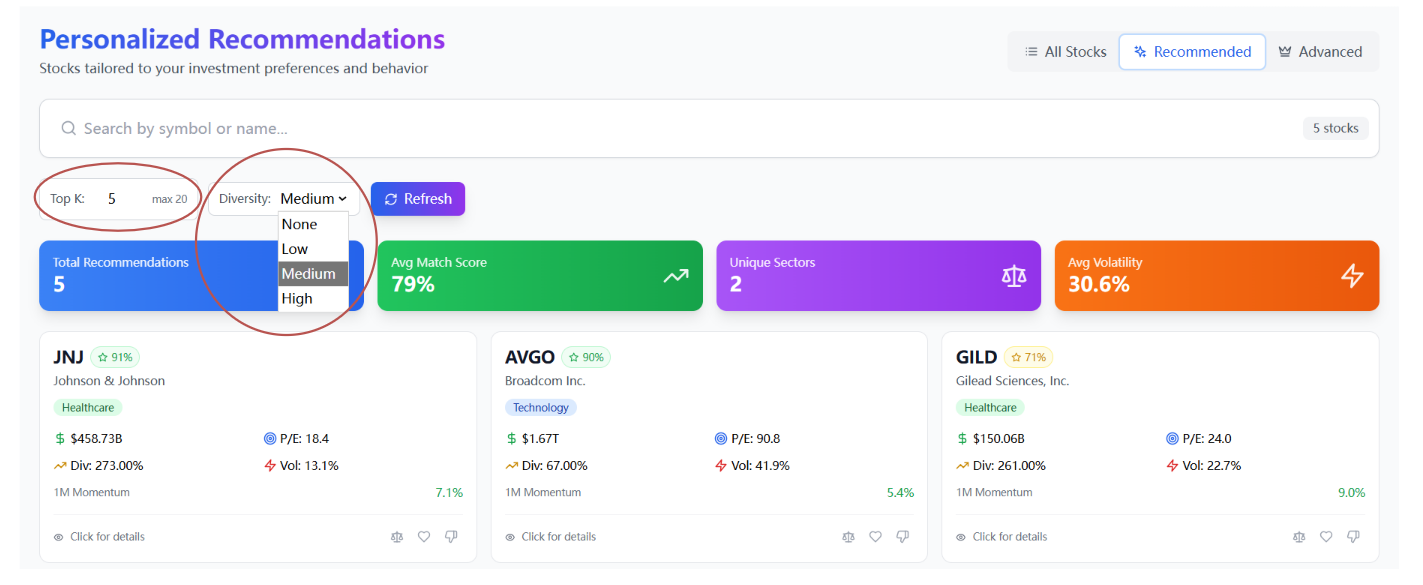
\includegraphics[width=1\linewidth]{images/stock_recommend/user_guide/basic_recommend.png}
    \caption{Basic Recommendation}
    \label{fig:basic_recommend}
\end{figure}


\subsection{Using Advanced Recommendations}
For multi-objective optimized recommendations, as Shown in Fig \ref{fig:advanced_recommend}:

\begin{enumerate}
    \item Click the \textbf{"Advanced"} tab
    \item Select your risk profile:
    \begin{itemize}
        \item \textbf{Conservative}: Lower risk, stable returns
        \item \textbf{Balanced}: Moderate risk and return balance
        \item \textbf{Aggressive}: Higher risk, potential for higher returns
    \end{itemize}
    \item View the detailed score breakdown for each recommendation:
    \begin{itemize}
        \item Final composite score
        \item Preference matching score
        \item Risk-adjusted return score
        \item Diversification benefit score
        \item Market timing score
    \end{itemize}
    \item Read the explanation for why each stock is recommended
    \item Adjust the number of recommendations using the \textbf{"Top K"} setting
\end{enumerate}

\begin{figure}[H]
    \centering
    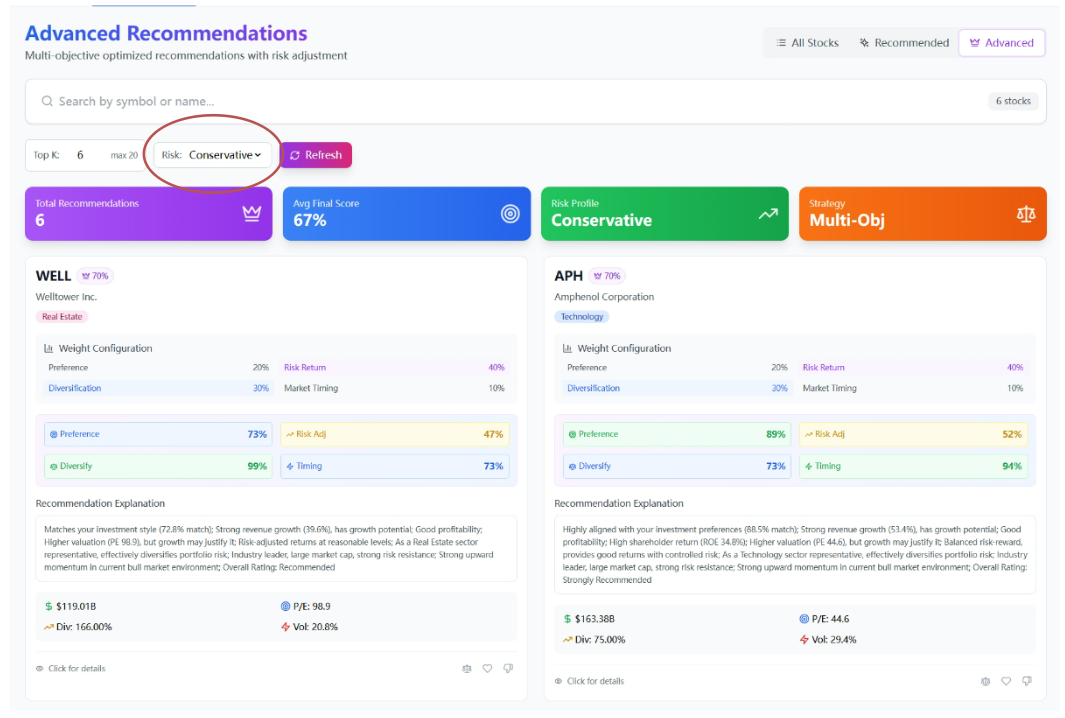
\includegraphics[width=1\linewidth]{images/stock_recommend/user_guide/advanced_recommend.png}
    \caption{Advanced Recommendation}
    \label{fig:advanced_recommend}
\end{figure}


\subsection{Comparing Stocks}
To compare multiple stocks side-by-side, as shown in Fig \ref{fig:stock_comparison}:

\begin{enumerate}
    \item Click the scale icon on any stock card to add it to comparison
    \item You can add up to 3 stocks for comparison
    \item View the comparison panel that appears at the top of the screen
    \item Click \textbf{"Analyze Comparison"} when you have 2 or more stocks selected
    \item In the comparison modal, you can:
    \begin{itemize}
        \item View side-by-side metrics in a comparison table
        \item Analyze valuation differences through bar charts
        \item Compare risk levels through volatility visualizations
        \item Review growth metric comparisons
        \item Read the summary analysis highlighting key differences
    \end{itemize}
    \item Remove stocks from comparison by clicking the 'x' button
\end{enumerate}
\begin{figure}[H]
    \centering
    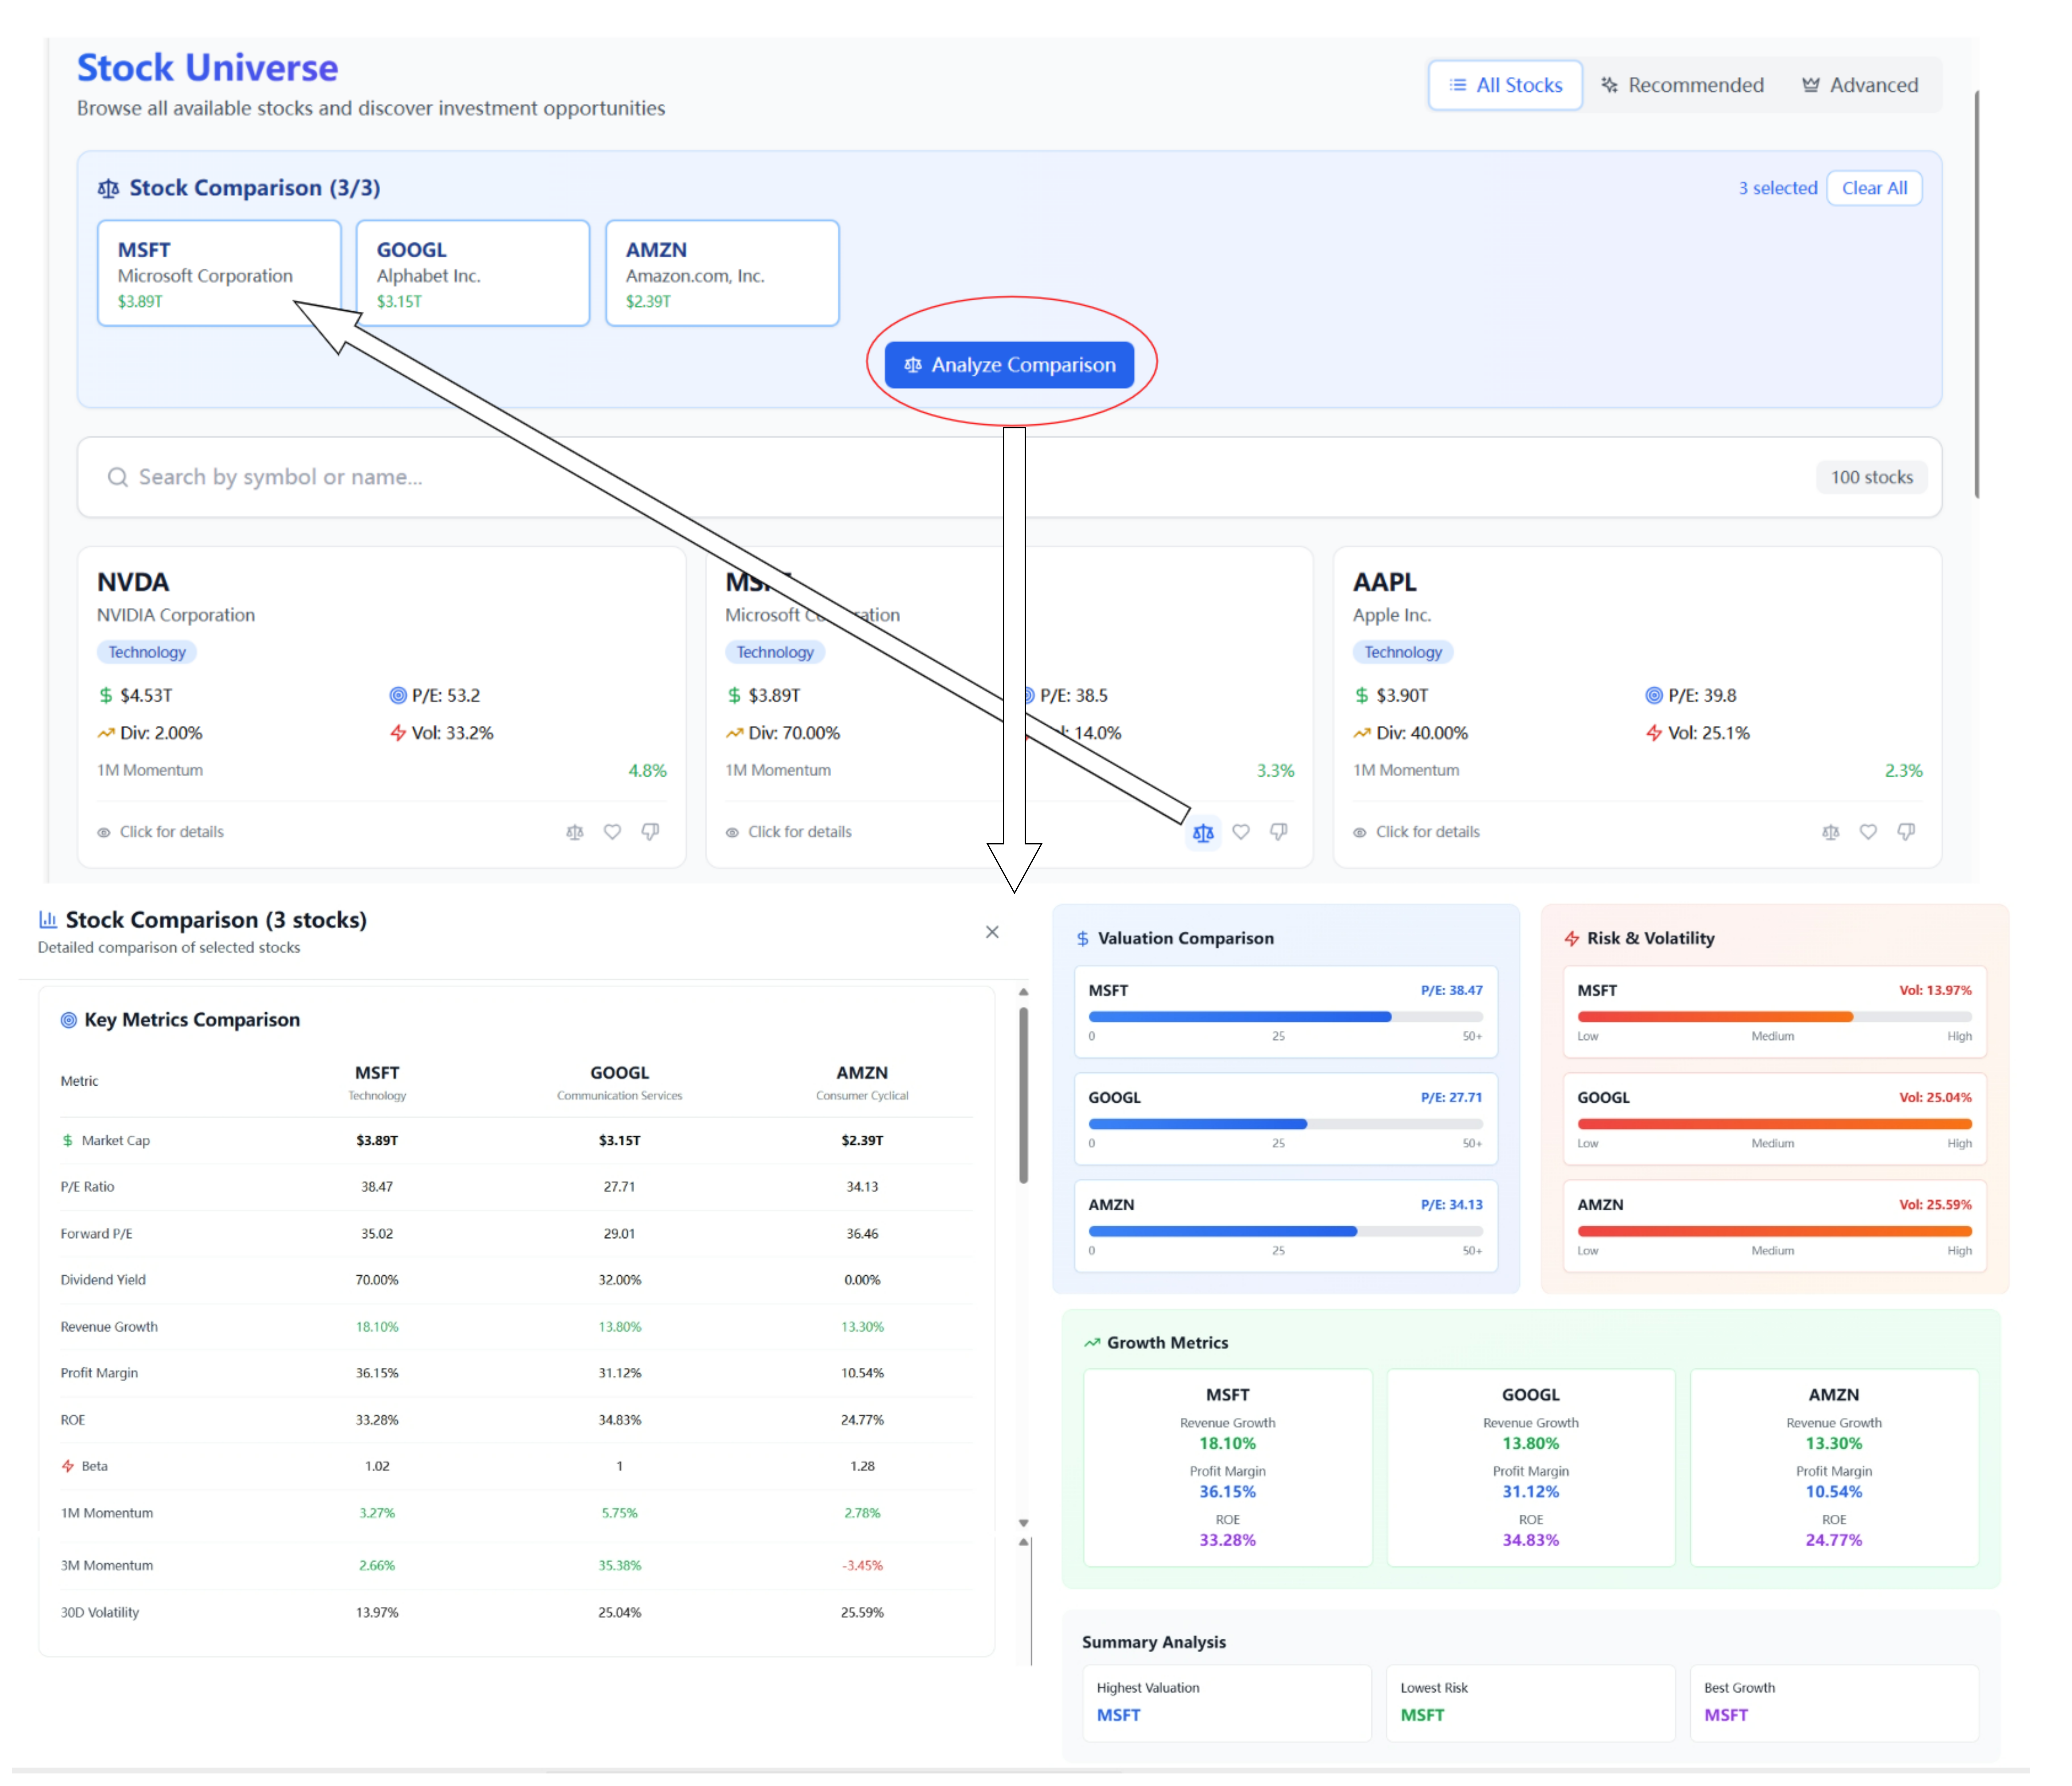
\includegraphics[width=1\linewidth]{images/stock_recommend/user_guide/compare.png}
    \caption{Stock Comparison}
    \label{fig:stock_comparison}
\end{figure}


\subsection{Viewing Stock Details}
To access comprehensive stock information, as shown in Fig \ref{fig:stock_detail}:

\begin{enumerate}
    \item Click on any stock card (except the action buttons)
    \item The stock detail modal will open with comprehensive information
    \item Navigate through different sections:
    \begin{itemize}
        \item \textbf{Price Charts}: Switch between time ranges (1M, 3M, 6M, 1Y) and price types (Close, Open, High, Low)
        \item \textbf{Valuation Metrics}: View P/E ratios, market cap, and other valuation data
        \item \textbf{Financial Ratios}: Analyze profitability, growth, and efficiency metrics
        \item \textbf{Dividend Information}: Review yield and payout ratios
        \item \textbf{Performance Metrics}: Check momentum and volatility data
        \item \textbf{Business Summary}: Read the company description
    \end{itemize}
\end{enumerate}

\begin{figure}[H]
    \centering
    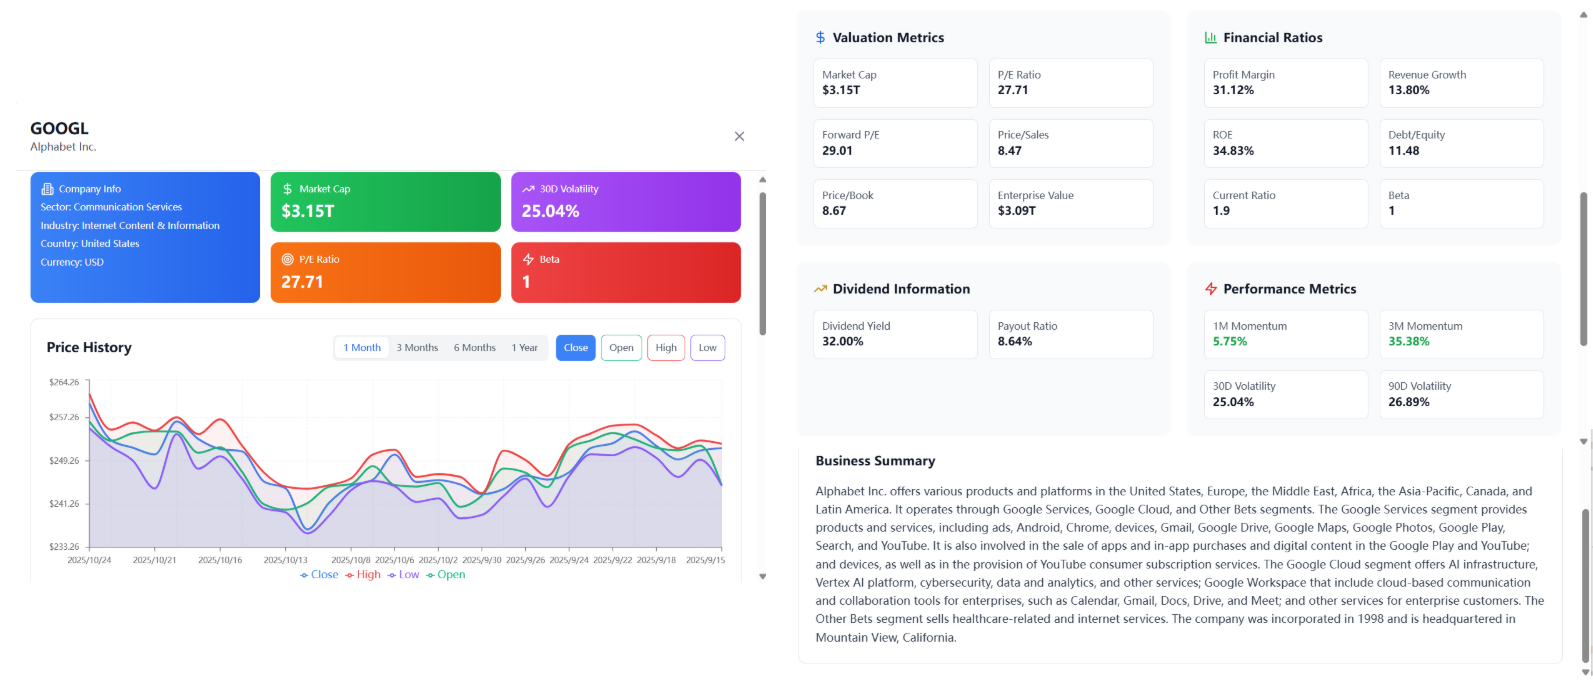
\includegraphics[width=1\linewidth]{images/stock_recommend/user_guide/stock_detail.png}
    \caption{Stock Detail}
    \label{fig:stock_detail}
\end{figure}

\subsection{Improving Recommendations Through Behavior}
The system learns from your interactions to provide better recommendations, as shown in Fig \ref{fig:like_dislike}:

\begin{enumerate}
    \item \textbf{Liking Stocks}: Click the heart icon ($\pmb{\heartsuit}$) on stocks you're interested in
    \begin{itemize}
        \item This tells the system you prefer similar stocks
        \item The heart will turn green and show a count
    \end{itemize}
    \item \textbf{Disliking Stocks}: Click the thumbs down icon on stocks you want to avoid
    \begin{itemize}
        \item This helps the system understand what to avoid recommending
        \item The icon will turn red and show a count
    \end{itemize}
    \item \textbf{Viewing Details}: Simply clicking on stocks to view details also influences your profile
    \item \textbf{Automatic Updates}: The system automatically:
    \begin{itemize}
        \item Updates your investment profile based on interactions
        \item Adjusts future recommendations in real-time
        \item Learns your sector preferences and investment style
    \end{itemize}
    \item To see the impact of your interactions, refresh the recommendations after several interactions
\end{enumerate}

\begin{figure}[H]
    \centering
    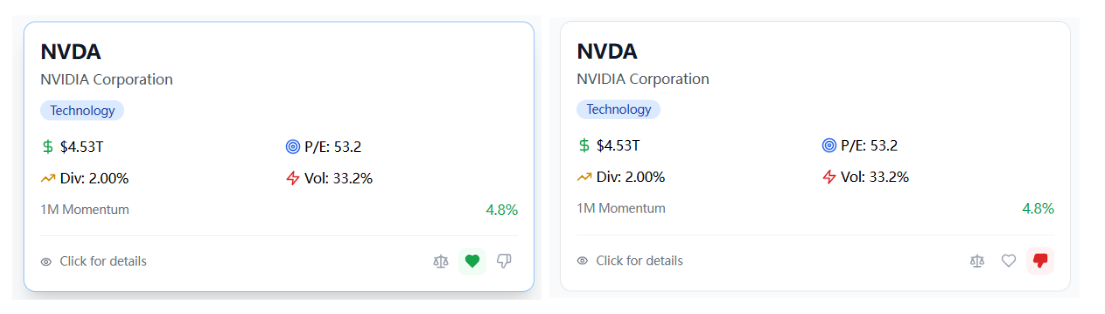
\includegraphics[width=1\linewidth]{images/stock_recommend/user_guide/like_dislike.png}
    \caption{User Behavior (like, dislike}
    \label{fig:like_dislike}
\end{figure}






\section{Stock Prediction}

\subsection{Overview}

The FinSight Stock Forecast Module provides users with intelligent, real-time stock trend predictions powered by multiple time-series and machine learning models.  
It visualizes both recent historical prices and short-term future forecasts, allowing users to intuitively interpret model predictions, confidence levels, and expected changes.  
This guide explains how to access, interact with, and interpret the stock forecasting interface.

\begin{figure}[H]
    \centering
    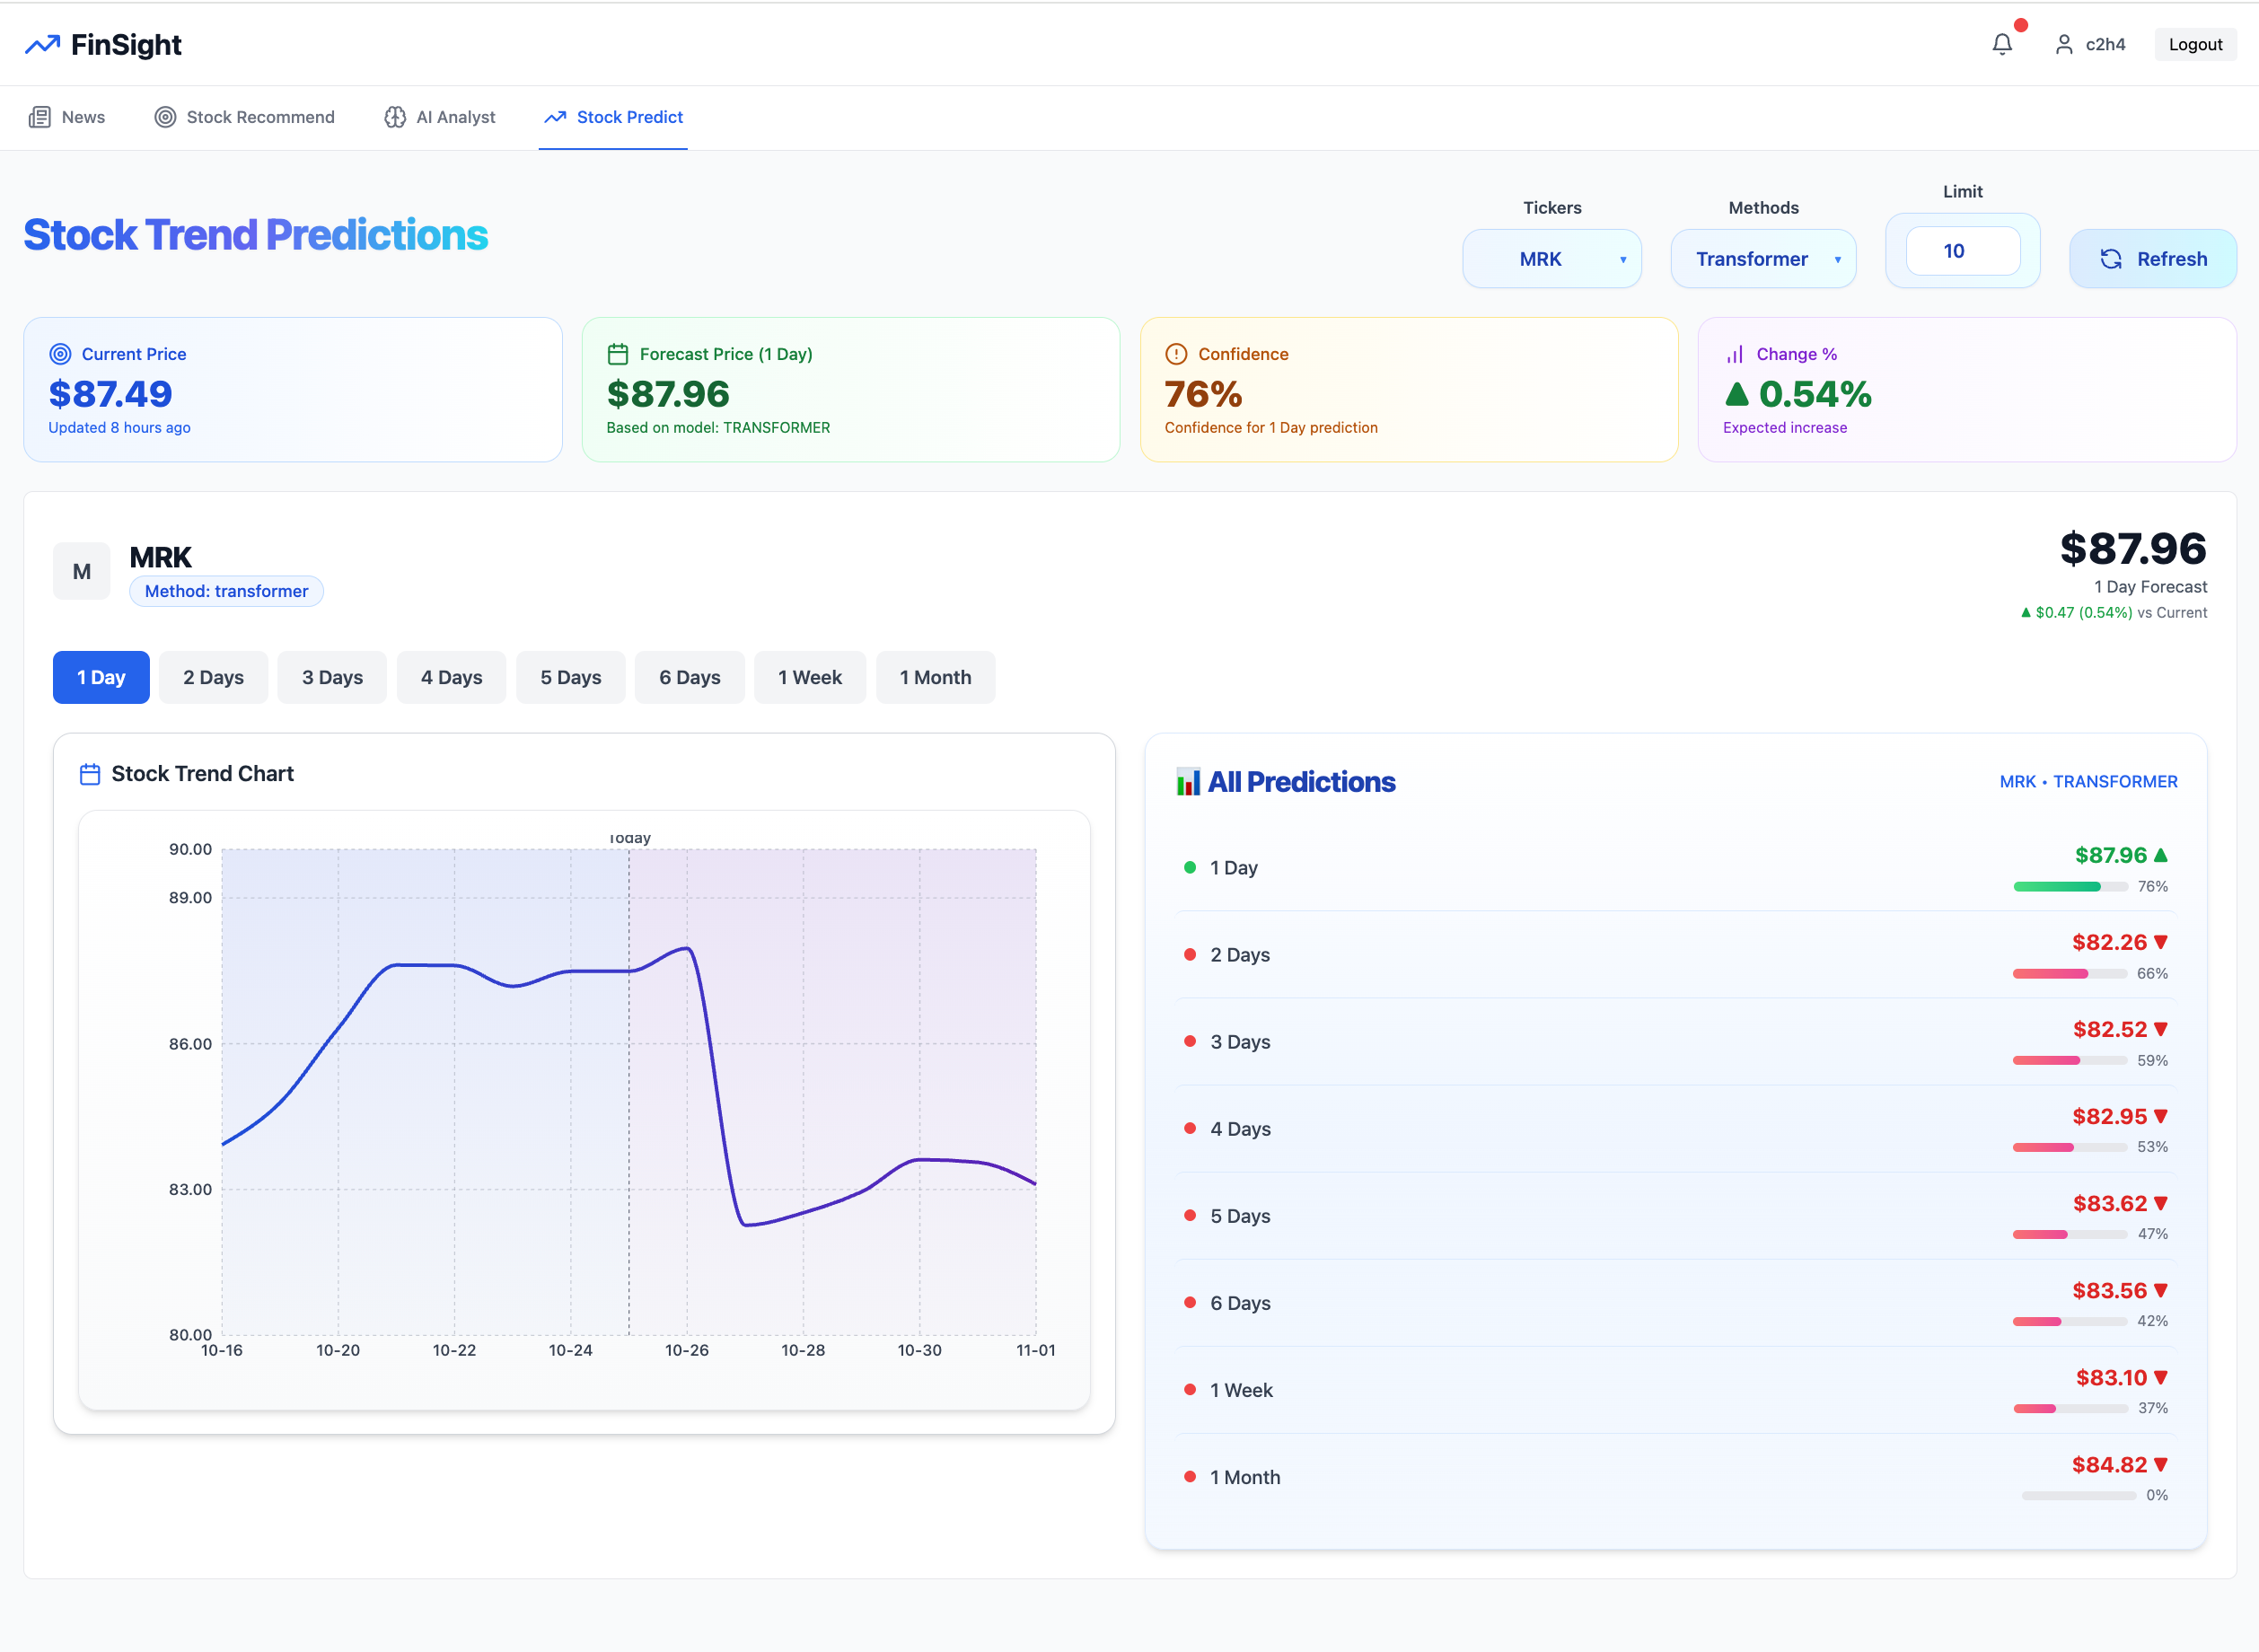
\includegraphics[width=1\linewidth]{images/prediction/overview.png}
    \caption{Stock Prediction User Interface}

\end{figure}

\subsection{Interface Overview}

\begin{enumerate}
  \item Open the FinSight web application in your browser.
  \item Log in using your registered account credentials.
  \item Navigate to the \textbf{“Stock Predict”} tab from the top navigation bar.
  \item Select a stock ticker (e.g., AAPL, TSLA, MRK) and a forecasting model (ARIMA, Prophet, LSTM, Transformer) from the dropdown menus.
  \item Click \textbf{Refresh} to load the most recent predictions and market data.
\end{enumerate}

Once loaded, the system displays the current price, forecasted price, model confidence, and expected percentage change in a clean and responsive dashboard.

\subsection{Understanding the Forecast Dashboard}

The main dashboard is divided into three functional regions for clarity and analytical insight:

\begin{itemize}
  \item \textbf{Top Summary Cards:}
    \begin{itemize}
      \item \textbf{Current Price:} Shows the latest closing price retrieved from the market data feed.
      \item \textbf{Forecast Price:} Displays the model’s predicted price for the selected horizon (e.g., 1 Day, 1 Week).
      \item \textbf{Confidence:} Indicates the model’s reliability, derived from validation metrics such as RMSE or variance.
      \item \textbf{Change} Shows the expected price movement relative to the current price, color-coded in green (positive) or red (negative).
    \end{itemize}
  \item \textbf{Trend Chart:}
    \begin{itemize}
      \item Visualizes both recent actual prices (solid blue line) and predicted prices (purple dashed line).
      \item A vertical line marks “today,” separating historical and forecasted data.
      \item Shaded areas represent confidence intervals for visualizing prediction uncertainty.
      \item Horizon buttons (1 Day, 3 Days, 1 Week, 1 Month) dynamically update the chart without reloading the page.
    \end{itemize}
  \item \textbf{Prediction Summary Panel:}
    \begin{itemize}
      \item Lists all horizon forecasts with predicted values, confidence scores, and trend arrows.
      \item Allows quick comparison between short-term and medium-term predictions.
      \item Color-coded bars visualize model confidence for each horizon.
    \end{itemize}
\end{itemize}

\subsection{Interacting with Forecasts}

You can explore predictions interactively:
\begin{itemize}
  \item Change the \textbf{ticker symbol} to analyze a different stock instantly.
  \item Switch between \textbf{models} (e.g., LSTM vs. Transformer) to compare forecast behavior.
  \item Adjust the \textbf{limit} or time horizon to view more or fewer prediction intervals.
  \item Hover over any data point in the chart to view exact date and price details.
\end{itemize}

All interactions automatically trigger backend API calls, and updated results appear within seconds.

\subsection{Interpreting Forecast Results}

\begin{itemize}
  \item A \textbf{higher confidence score} (close to 100\%) indicates a more stable forecast, while lower scores reflect market volatility or data uncertainty.
  \item Positive \textbf{Change \%} suggests an expected upward trend; negative values suggest possible price declines.
  \item Comparing multiple models provides insight into how traditional and deep learning approaches interpret market patterns differently.
  \item The chart’s shaded area width visually represents prediction risk—the wider the band, the greater the uncertainty.
\end{itemize}

\subsection{Tips for Best Experience}

\begin{itemize}
  \item Refresh periodically to fetch the most recent forecast data.
  \item Compare different models to assess prediction consistency.
  \item Use shorter horizons (1\–3 days) for near-term signals and longer ones for trend analysis.
  \item Interpret low-confidence predictions cautiously; they indicate volatile or sparse underlying data.
  \item Combine forecast insights with other FinSight modules for more informed investment decisions.
\end{itemize}




\section{AI Analyst}

The \textbf{AI Financial Analyst} module serves as an intelligent assistant powered by a Retrieval-Augmented Generation (RAG) framework. 
It enables users to ask analytical questions about stocks, sectors, earnings, and market trends, and receive context-aware, knowledge-grounded answers.
\begin{figure}[H]
    \centering
    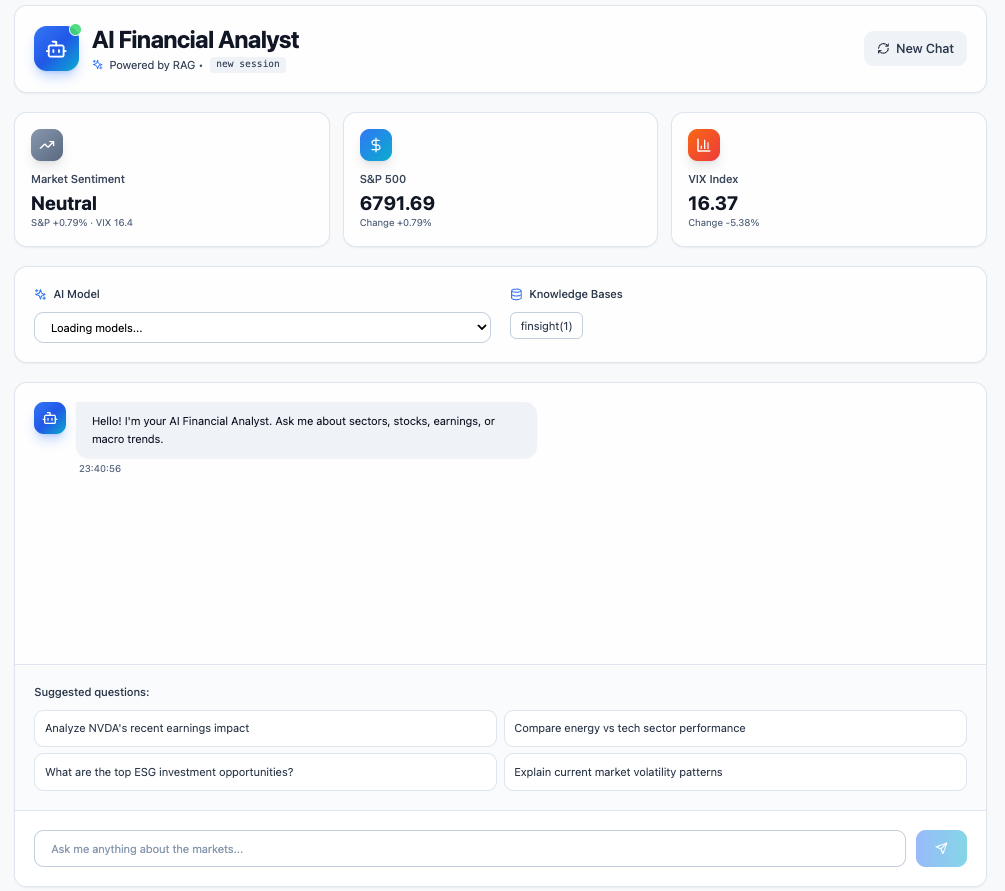
\includegraphics[width=1\linewidth]{images/AI_Analyst_interface.png}
    \caption{AI Analyst User Interface}
    \label{fig:placeholder}
\end{figure}
\subsection{Interface Overview}

\begin{itemize}
    \item \textbf{Market Indicators} \\
    The dashboard displays key real-time market metrics:
    \begin{itemize}
        \item \textbf{Market Sentiment:} General market mood derived from aggregated financial data.
        \item \textbf{S\&P 500 Index:} Current value and daily percentage change of the U.S. benchmark index.
        \item \textbf{VIX Index:} Market volatility indicator reflecting overall risk and uncertainty levels.
    \end{itemize}

    \item \textbf{AI Model Selection} \\
    Users can choose among available AI models (e.g., deepSeek-r1:8b) to power the assistant’s reasoning and response generation.

    \item \textbf{Knowledge Base Selection} \\
    The system allows users to select from available financial knowledge bases (e.g., \textit{finsight(1)}). 
    The selected dataset determines the retrieval source used to ground responses with relevant and accurate financial context.
\end{itemize}

\subsection{Functionality}

The AI Analyst supports natural-language financial Q\&A, allowing users to:
\begin{itemize}
    \item Ask about market movements, company performance, or sector comparisons.
    \item Obtain summarized insights, reasoning explanations, and evidence-based references.
    \item Conduct context-aware, multi-turn analytical conversations supported by the selected model and knowledge base.
\end{itemize}

		
\pagestyle{nuspageback}

% {\backmatter
% 	% Bibliography
% 	\if@openright\cleardoublepage\else\clearpage\fi
% 	% Use something like https://flamingtempura.github.io/bibtex-tidy/ to clean all your bibtex entries
% 	\printbibliography[title=References]
% 	\printindex
% }
	
\end{document}

%%% The End %%%
